%%%
%\documentclass[10pt, a4paper]{report}
%\documentclass[12pt, a4paper]{article}
\documentclass[11pt, a4paper]{book}
%%%\documentclass[12pt, b5paper, draft]{report}
%%%\documentclass[10pt, a4paper, twocolumn]{book}
%%%\documentclass[10pt, a4paper]{book}

\usepackage[english]{babel}
\usepackage[left=2.5cm,right=2.5cm,top=3cm,bottom=3.5cm]{geometry}
%%\usepackage[top=3cm,bottom=2cm,inner=2.5cm,outer=1.5cm]{geometry}
%\usepackage[small]{titlesec}
\usepackage{enumitem}
\usepackage[affil-it]{authblk}
\usepackage{graphicx}
\usepackage{wrapfig}
\usepackage{xcolor}
\usepackage{subfigure}
\usepackage{float}
\usepackage{amsmath}
\usepackage{amssymb}
\usepackage{fancyhdr}
\usepackage{lineno}
\usepackage[bookmarks]{hyperref}
\usepackage{cite}
\usepackage{titling}
\usepackage{mdframed}
\usepackage[most]{tcolorbox}
\usepackage{sectsty}
\usepackage{tikz-feynman}
\usepackage{multicol}
\usepackage[explicit]{titlesec}
\usepackage{etoolbox}
\usepackage{xspace}
\usepackage{gensymb}
\usepackage{arydshln}
%\usepackage[utf8]{inputenc}
\makeatletter
\patchcmd{\ttlh@hang}{\parindent\z@}{\parindent\z@\leavevmode}{}{}
\patchcmd{\ttlh@hang}{\noindent}{}{}{}
\makeatother
%%%\usepackage[many]{tcolorbox}
\chapterfont{\color{red!80!black}\bf\textit}%
%\chapterfont{\color{white}\bf\textit}%
\pagestyle{fancy}
%%\addtolength{\headwidth}{\marginparsep}
%%\addtolength{\headwidth}{\marginparwidth}

\renewcommand{\chaptermark}[1]{\markboth{#1}{}}
\renewcommand{\sectionmark}[1]{\markright{\thesection\ #1}}

\fancyhf{}
\fancyhead[LO]{\bfseries\rightmark}
\fancyhead[RE]{\bfseries\leftmark}
\fancyfoot[LE,RO]{\bfseries \thepage}
\fancypagestyle{plain}{%
%%\fancyhead{} % leva l’intestazione
\renewcommand{\headrulewidth}{0pt} % e la linea da inizio capitolo
}

%%%layout decorations:
%%\renewcommand{\headrulewidth}{1.4pt}
%%\renewcommand{\footrulewidth}{0.4pt}

%%\renewcommand\footrule{\begin{minipage}{1\textwidth}
%%\hrule width \hsize height 2pt \kern 1mm \hrule width \hsize   
%%\end{minipage}\par}%

\renewcommand\headrule{
\begin{minipage}{1\textwidth}
\hrule width \hsize \kern 1mm \hrule width \hsize height 2pt 
\end{minipage}}%

\renewcommand{\footrulewidth}{0.4pt}

%%%font style
%%\renewcommand{\familydefault}{\sfdefault}
%%\renewcommand*\sfdefault{ppl}
%%\renewcommand*\sfdefault{iwona}

%%\renewcommand{\familydefault}{\rmdefault}
%%\renewcommand*\rmdefault{ppl}
%%\renewcommand*\rmdefault{iwona}

%%\renewcommand{\familydefault}{\ttdefault}

%%%others:
%%barocco
%\usepackage{gfsartemisia-euler}
%\usepackage[T1]{fontenc}
%% un po' schiacciato
%\usepackage[sfmath]{kpfonts}
%\renewcommand*\familydefault{\sfdefault}
%\usepackage[T1]{fontenc}
%%
% Troppo pesante da leggere
%\usepackage[default]{gfsneohellenic}
%\usepackage[LGR,T1]{fontenc} %% LGR encoding is needed for loading the package gfsneohellenic
%% particolare, ma poco leggibile...:
%\usepackage[math]{iwona}
%\usepackage[T1]{fontenc}
%%


%% ben leggibile, scelto, ma uguale ad Alberto:
%\usepackage[sc]{mathpazo}
%\linespread{1.05}         % Palladio needs more leading (space between lines)
%\usepackage[T1]{fontenc}



%%insomma, non troppo carino:
%\usepackage{fouriernc}
%\usepackage[T1]{fontenc}
%%
%abbastanza standard, piu' schiacciato ma non bad:
\usepackage[adobe-utopia]{mathdesign}
\usepackage[T1]{fontenc}


%CMS symbols

%

\definecolor{titlebgdark}{RGB}{0,163,243}
\definecolor{titlebglight}{RGB}{191,233,251}

\titleformat{\chapter}[display]
  {\normalfont\Huge\bfseries}
  {}
  {20pt}
  {%
    \begin{tcolorbox}[
      enhanced,
      colback=black!5!white,
      boxrule=0.25cm,
      colframe=black!15!white,
      arc=0pt,
      outer arc=0pt,
      leftrule=0pt,
      rightrule=0pt,
      fontupper=\color{red!80!black},
      enlarge left by=-1in-\hoffset-\oddsidemargin, 
      enlarge right by=-\paperwidth+1in+\hoffset+\oddsidemargin+\textwidth,
      width=\paperwidth, 
      left=1in+\hoffset+\oddsidemargin, 
      right=\paperwidth-1in-\hoffset-\oddsidemargin-\textwidth,
      top=0.6cm, 
      bottom=0.6cm,
      overlay={
        \node[
          fill=black!5!white,
          draw=black!15!white,
          line width=0.15cm,
          inner sep=0pt,
          text width=1.7cm,
          minimum height=1.7cm,
          align=center,
          font=\Huge\color{red!80!black}
        ] 
        (chapname)
        at ([xshift=-4cm]frame.north east)
        {\thechapter};
        \node[font=\normalsize\color{red!80!black},anchor=south,inner sep=2pt] at (chapname.north)
        {\chaptertitlename};  
      } 
    ]
    #1
    \end{tcolorbox}%
  }
\titleformat{name=\chapter,numberless}[display]
  {\normalfont\huge\bfseries}
  {}
  {20pt}
  {%
    \begin{tcolorbox}[
      enhanced,
      colback=black!5!white,
      boxrule=0.25cm,
      colframe=black!15!white,
      arc=0pt,
      outer arc=0pt,
      remember as=title,
      leftrule=0pt,
      rightrule=0pt,
      fontupper=\color{red!80!black}\huge,
      enlarge left by=-1in-\hoffset-\oddsidemargin, 
      enlarge right by=-\paperwidth+1in+\hoffset+\oddsidemargin+\textwidth,
      width=\paperwidth, 
      left=1in+\hoffset+\oddsidemargin, 
      right=\paperwidth-1in-\hoffset-\oddsidemargin-\textwidth,
      top=0.6cm, 
      bottom=0.6cm, 
    ]
    #1
    \end{tcolorbox}%
  }
\titlespacing*{\chapter}
  {0pt}{0pt}{40pt}
\makeatother

\newcommand{\pt}{\ensuremath{p_T}\xspace}
\newcommand{\kt}{\ensuremath{k_T}\xspace}
\newcommand{\PZ}{\text{Z}\xspace}
\newcommand{\PW}{\text{W}\xspace}
\newcommand{\cm}{\text{cm}\xspace}
\newcommand{\GeV}{\text{GeV}\xspace}
\newcommand{\TeV}{\text{TeV}\xspace}
\newcommand{\tev}{\text{TeV}\xspace}
\newcommand{\fb}{\text{fb}\xspace}
\newcommand{\pb}{\text{pb}\xspace}
\newcommand{\invfb}{\text{fb}^{-1}\xspace}
\newcommand{\invpb}{\text{pb}^{-1}\xspace}
\newcommand{\pbinv} {\mbox{\ensuremath{\,\text{pb}^\text{$-$1}}}\xspace}
\newcommand{\fbinv} {\mbox{\ensuremath{\,\text{fb}^\text{$-$1}}}\xspace}
\newcommand{\rap}{\ensuremath{\mathcal{Y}}\xspace}
\newcommand{\met}{\ensuremath{\vec{p}_T^{\text{miss}}}\xspace}
\newcommand{\MET}{\ensuremath{E_T^{\text{miss}}}\xspace}
\newcommand{\VZ}{\ensuremath{VZ}\xspace}
\newcommand{\W}{\ensuremath{W}\xspace}
\newcommand{\Z}{\ensuremath{Z}\xspace}
\newcommand{\V}{\ensuremath{V}\xspace}
\newcommand{\VV}{\ensuremath{VV}\xspace}
\newcommand{\G}{\ensuremath{G}\xspace}
\newcommand{\Wp}{\ensuremath{W'}\xspace}
\newcommand{\HT}{\ensuremath{H_{\mathrm{T}}}\xspace}
\newcommand{\VZinv}{\ensuremath{VZ \rightarrow q \bar{q} \nu \bar{\nu}}\xspace}
\newcommand{\BGinv}{\ensuremath{G \rightarrow ZZ \rightarrow q \bar{q} \nu \bar{\nu}}\xspace}
\newcommand{\Wpinv}{\ensuremath{W' \rightarrow WZ \rightarrow q \bar{q}' \nu \bar{\nu}}\xspace}
\newcommand{\mtVZ}{\ensuremath{m_{\VZ}^T}\xspace}
\newcommand{\mVZ}{\ensuremath{m_{\VZ}}\xspace}
\newcommand{\mX}{\ensuremath{m_{X}}\xspace}
\newcommand{\ttbar}{\ensuremath{t \bar{t}}\xspace}

\newcommand{\PYTHIA} {{\textsc{pythia}}\xspace}
\newcommand{\MADGRAPH} {\textsc{MadGraph}\xspace}
\newcommand{\POWHEG} {{\textsc{powheg}}\xspace}
\newcommand{\MCATNLO} {\textsc{mc@nlo}\xspace}
\newcommand{\GEANTfour} {{\textsc{Geant4}}\xspace}

\setcounter{secnumdepth}{4}
\setcounter{tocdepth}{4}

\title{Search for heavy resonances decaying into a $Z$ boson and a vector boson in the $\nu \bar{\nu}$ $q\bar{q}$ final state at CMS}

\date{}
\author{Supervisor: Prof. Franco Simonetto \\ Candidate: Lisa Benato} %, {\itshape Universit\`a degli studi di Padova}}
\affil{Universit\`a degli studi di Padova}


\begin{document}

\begin{titlingpage} %This starts the title page
\begin{center}

\includegraphics[height=3.5cm]{logo}\\ %Put the logo you want here
\begin{large}
Universit\`a degli studi di Padova \\ %The name your university
Dipartimento di Fisica e Astronomia\\
\end{large}
\vspace{1.5cm} %You can control the vertical distance
\begin{large}
Tesi di Dottorato \\
\end{large}
\vspace{1.5cm}
\begin{tcolorbox}[breakable,colback=black!5!white,colframe=red!80!black,width=\textwidth]
\begin{center}
\begin{Huge} 
{\color{red!80!black}\textbf{\thetitle}} \\
\end{Huge}
\end{center}
\end{tcolorbox}
\vspace{3.5cm}
\theauthor\\
\vspace{5cm} %Put the distance you need.
Scuola di Dottorato di Ricerca, XXX ciclo
%\thedate
\end{center}
\end{titlingpage}

%\maketitle
\newpage\null\thispagestyle{empty}\newpage
\thispagestyle{empty}
\begin{flushright}
\null\vspace{\stretch{1}}
%Joy in looking and comprehending is nature's most beautiful gift.
"I have no special talent. I am only passionately curious."\\
(A. Einstein)
\vspace{\stretch{2}}\null
\end{flushright}

\newpage\null\thispagestyle{empty}\newpage
\thispagestyle{empty}

\frontmatter %numeri romani
\tableofcontents

\linenumbers
\chapter*{Abstract} 
\mainmatter %numeri arabi da qui in poi

\chapter{Introduction}%Dummy
%\chapter{Introduction}

The discovery of the Higgs boson at the CERN Large Hadron Collider represents a milestone in the knowledge of the particle physics. The Higgs mechanism connects the theoretical formulation of the standard model of the particles to the current picture of the universe, as it is known: spin-1 weak bosons and standard model fermions are allowed to acquire masses, constituting the fundamental bricks of the known matter. Despite this successful achievement, some questions are still left unanswered; in order to solve the open problems, a plethora of new beyond standard model theories has been built.

\noindent Many of these theories hypothesize the existence of larger symmetries in the universe, or new extra-dimensions, that will result into the appearance of new heavy particles, expected to have masses around the \TeV scale. The Large Hadron Collider (LHC) is the ideal tool to investigate this unknown phase-space, given the fact that during the so-called LHC Run 2 era (started in 2015), the unprecedented center-of-mass energy of 13 \TeV has been reached in the proton-proton collisions.

\noindent The CMS experiment, located in the northern part of the LHC ring, is a multi-purpose detector, suitable to study highly energetic new phenomena. Its intense magnetic field, its sharp segmentation, its hermeticity and the interplay of many sophisticated reconstruction algorithms allow to measure with a very high precision the trajectories, the momenta and the energy deposits left by energetic particles.

\vspace*{1\baselineskip}

\noindent This thesis presents a search for signals of heavy resonances that decay into a pair of vector bosons. The search is performed by using the 2016 data produced by proton-proton collisions of the LHC, and collected by the CMS detector. One $Z$ boson is identified through its invisible decay in neutrinos, while the other vector boson is required to decay hadronically into a pair of quarks. Given the fact that the searched resonances have masses around the \TeV, their decay products are expected to be produced with large Lorentz boosts. This leads to a non-trivial identification of the couple of quarks or leptons, coming from the vector bosons decays. In fact, they are expected to lie very close in angle. Dedicated algorithms and substructure techniques allow to distinguish a pair of quarks originating from a vector boson from the background processes, initiated by the strong interaction.

\noindent The search is performed by scanning the distribution of the reconstructed mass of the resonance, looking for a local excess in data with regards to the predictions. The background estimation is performed with an hybrid data-simulation approach, by using the distribution of data in signal-depleted control regions.

\newpage

\noindent The thesis is organized as follows.

\vspace*{1\baselineskip}

\noindent In chapter~\ref{chap:theory}, an overview of the theoretical motivations is presented. Two beyond standard model theories are considered: the Heavy Vector Triplet model and the bulk graviton model, a particular scenario included in warped extra-dimensions theories. In both cases, new heavy particles are expected to decay into vector bosons with a sizeable rate.

\vspace*{1\baselineskip}

\noindent In chapter~\ref{chap:LHC_CMS}, the CMS detector is briefly described, along with the physics objects exploited for the purpose of this search.

\vspace*{1\baselineskip}

\noindent Chapter~\ref{ch:analysis} is dedicated to the analysis: after a general introduction (sec.~\ref{sec:analysis_overview}), the features of the data, signal and background samples used in the analysis are described in detail (sec.~\ref{sec:samples}). Sec.~\ref{sec:objects} is dedicated to the selections applied, in order to reach the best signal-to-noise efficiency and to properly build the resonance candidate. The very first data-simulation comparison is performed in sec.~\ref{sec:datamc_comp}. The background estimation technique, the final data-predicted background comparison and the signal modelling are included in sec.~\ref{sec:alpha}. Systematic uncertainties are listed in sec.~\ref{sec:uncertainties}. The final results, the statistical analysis and the physics interpretation are shown in sec.~\ref{sec:results}.

\vspace*{1\baselineskip}

\noindent Chapter~\ref{ch:conclusion} summarizes the conclusions.

\clearpage



\chapter{Theoretical motivation}%Dummy
%%\begin{tcolorbox}[breakable,colback=black!5!white,colframe=red!80!black,width=\textwidth]
%%\begin{tcolorbox}[breakable,colback=black,colframe=black,width=\textwidth]
\chapter{Theoretical motivation}
%\end{tcolorbox}
\label{chap:theory}

The standard model (SM) of elementary particles represents, so far, the best available description of the particles and their interactions. It is the summation of two gauge theories: the electroweak interaction, that portrays the weak and electromagnetic interactions together, and the strong interaction, or Quantum Chromodynamics (QCD). Particles, namely quarks and leptons, are described as spin 1/2 fermions, whilst interactions are mediated by spin 1 bosons. The symmetry group of the standard model is:
\begin{equation}
SU_{C}(3) \times SU_L (2) \times U_Y (1),
\end{equation}
\label{eq:theory_SMgroup}
\noindent where the first factor is related to strong interactions, whose mediators are eight gluons, while $SU_L (2) \times U_Y (1)$ is the electroweak simmetry group, whose mediators are the photon and $Z$-$W^{\pm}$ bosons.\\
In renormalizable theories, with no anomalies, all gauge bosons are expected to be massless, in contrast with our experimental knowledge. This inconsistency is solved by introducing a new scalar particle, the Higgs boson, that gives mass to weak bosons and fermions via the spontaneous symmetry breaking mechanism.
\\

\noindent In the last decades, the standard model has been accurately probed by many experimental facilities (LEP, Tevatron. LHC), and the results lead to an impressive agreement between theoretical predictions and experiments~\cite{Baak:2013ppa}. The discovery of the Higgs boson at the CERN Large Hadron Collider, measured by both CMS and ATLAS collaborations~\cite{bib:Aad20121,bib:Chatrchyan201230,bib:Chatrchyan2013lba,Aad:2013xqa,Khachatryan:2014jba,Aad:2014aba,Aad:2015zhl}, represents not only an extraordinary confirmation of the model, but also the latest biggest achievement in particle physics as a whole.

\section{Beyond standard model theories}
Even though the SM is the most complete picture of the universe of the particles, many questions are still left open. From a phenomenological point of view, some experimental observations are not included in the theory:
\begin{itemize}
\item in SM, neutrinos are massless (whilst the well established observation of neutrino flavour oscillation proves that neutrinos do carry mass);
\item no candidates for dark matter are predicted;
\item no one of the fields included in the SM can explain the cosmological inflation;
\item the CP asymmetry embedded in the SM is not sufficient to explain the matter-antimatter asymmetry in the universe.
\end{itemize}
From a purely theoretical perspective, some issues are still relevant in the formulation of the model:
\begin{itemize}
\item {\itshape Flavour problem.}\\ The standard model has 18 free parameters: 9 fermionic masses; 3 angular parameters in Cabibbo-Kobayashi-Maskawa matrix, plus 1 phase parameter; electromagnetic coupling $\alpha$; strong coupling $\alpha_{\text{strong}}$;  weak coupling $\alpha_{\text{weak}}$; $Z$ mass; the mass of the Higgs boson. Such a huge number of degrees of freedom marks the SM as weakly predictive in the flavour sector.
\item {\itshape Unification.}\\ There is not a ``complete'' unification of strong, weak and electromagnetic interactions, since each one has its own coupling constant, behaving differently at different energy scales; not to mention the fact that gravitational interaction is completely excluded from the SM.
\item {\itshape Hierarchy problem.}\\ From Quantum Field Theory, it is known that perturbative corrections to the mass of the scalar bosons included in the theory tend to make it increase towards the energy scale at which the considered theory still holds~\cite{Degrassi:2012ry}. If the standard model is seen as a low-mass approximation of a more general theory valid up to the Planck mass scale (\textit{i.e.},~$\sim~1.2~\times~10^{19}$~GeV), a fine-tuning cancellation of the order of $1$ over $10^{34}$ is needed in order to protect the Higgs mass at the electroweak scale ($\sim 100$ GeV). Such an astonishing correction is perceived as very unnatural.
\end{itemize}

\noindent Numerous beyond standard model theories (BSM) have been proposed in order to overcome the limits of the SM.\\
Grand Unified Theories (GUT) aim at extending the symmetry group of the SM (eq.~\ref{eq:theory_SMgroup}) into largest candidates, such as $S0(10)$, $SU(5)$ and $E(6)$. At GUT scale, approximately at $10^{16}$ GeV, non-gravitational interactions are expected to be ruled by only one coupling constant, $\alpha_{GUT}$.\\%Pur godendo di alcuni punti di forza, quali la possibilit\`a di dare massa ai neutrini ammettendo l'esistenza del neutrino right alla scala GUT, queste teorie prevedono in alcuni casi fenomeni non ancora osservati (decadimento del protone, esistenza dei monopoli magnetici) e sono valide ad energie non riproducibili sperimentalmente. Qualche speranza di trovare nuova fisica a scale inferiori potrebbe nascere dal connubio tra GUT e modelli supersimmetrici.
Super Symmetryc (SUSY) models~\cite{Martin:1997ns} state that every fermion (boson) of the SM has a bosonic (fermionic) superpartner, with exactly the same quantum numbers, except the spin. If SUSY is not broken, each couple of partners and superpartners should have the same masses, hypothesis excluded by the non-observation of the s-electron. Super Symmetry represents a very elegant solution of the hierarchy problem of the Higgs boson mass, since the perturbative corrections brought by new SUSY particles exactly cancel out the divergences caused by SM particles corrections. A particular sub-class of SUSY models, minimal super symmetric standard models~\cite{Csaki:1996ks,Castano:1993ri,Haber:1993wf}, is characterized by the introduction of a new symmetry, the R-parity, that guarantees the proton stability and also the stability of the lightest SUSY particle, a possible good candidate for dark matter.
\\

\noindent Two other possible theoretical pictures are extensively described in sec.~\ref{sec:theory_HVT}-\ref{sec:theory_WED}.

\newpage

\section{Heavy Vector Triplet}
\label{sec:theory_HVT}

The heavy vector triplet model~\cite{Pappadopulo2014} provides a general framework aimed at studying new physics beyond the standard model, that can manifest into the appearance of new resonances.\\
The adopted approach is that of the simplified model, in which an effective Lagrangian is introduced, in order to describe the properties and interactions of new particles (in this case, a triplet of spin-1 bosons) by using a limited set of parameters, that can be easily linked to the physical observables at the LHC experiments. These parameters can describe many physical motivated theories (such as sequential extensions of the SM~\cite{Barger:1980ix,Grojean:2011vu} or Composite Higgs~\cite{Contino2011,Bellazzini:2014yua}), built to solve the hierarchy problem of the SM. \\
Since a simplified model is not a complete theory, its validity is restricted to the on-shell quantities related to the production and decay mechanisms of the new resonances, that is how most of the LHC BSM searches are performed. Given these conditions, experimental results in the resonant region are sensitive to a limited number of the phenomenological Lagrangian parameters (or to a combination of those), whilst the remaining parameters tend to influence the tail of the distributions.\\
Limits on production cross-section times branching ratio ($\sigma \mathcal{B}$), as a function of the invariant mass spectrum of the probed resonance, can be extracted from experimental data. Given that $\sigma \mathcal{B}$ are functions of the simplified model parameters and of the parton luminosities, it is then possible to interpret the observed limits in the parameter space.

\subsection{Simplified Lagrangian}
\label{sec:HVT_lagr}

The heavy vector triplet framework assumes the existence of an additional vector triplet, $V_{\mu}^a$, $a=1,2,3$, in which two spin-1 particles are charged and one is neutral:

\begin{equation}
\begin{split}
& V_{\mu}^{\pm} = \frac{V_{\mu}^1 \mp i V_{\mu}^2}{\sqrt{2}};\\
& V_{\mu}^0 = V_{\mu}^3.\\
\end{split}
\label{eq:V_triplet}
\end{equation}
\\
The triplet interactions are described by a simplified Lagrangian, that is invariant under SM gauge and CP symmetry, and accidentally invariant under the custodial symmetry $SU(2)_L \times SU(2)_R$:
\begin{equation}
\begin{split}
\mathcal{L_V} ={} & -\frac{1}{4} \left(D_{\mu}V_{\nu}^a - D_{\nu}V_{\mu}^a \right) \left( D^{\mu}V^{\nu \mbox{ } a} - D^{\nu}V^{\mu \mbox{ } a} \right) + \frac{m_V^2}{2}V_{\mu}^aV^{\mu \mbox{ } a} \\
 & +i g_V c_H V_{\mu}^a \left( H^{\dagger} \tau^a D^{\mu}H - D^{\mu}H^{\dagger} \tau^a H \right) + \frac{g^2}{g_V}c_F V_{\mu}^a \sum_{f} \bar{f}_L \gamma^{\mu} \tau^a f_L \\
 & + \frac{g_V}{2} c_{VVV} \epsilon_{abc} V_{\mu}^a V_{\nu}^b \left( D^{\mu}V^{\nu \mbox{ } c} - D^{\nu}V^{\mu \mbox{ } c}\right) + g_V^2 c_{VVHH} V_{\mu}^a V^{\mu \mbox{ } a} H^{\dagger} H - \frac{g}{2} c_{VVW} \epsilon_{abc} W^{\mu \nu \mbox{ } a} V_{\mu}^b V_{\nu}^c.
\end{split}
\label{eq:Lagrangian}
\end{equation}
\\
In the first line of the formula~\ref{eq:Lagrangian}, $V$ mass and kinematic terms are included, described with the covariant derivative $D_{\mu} V_{\nu}^a = \partial_{\mu} V_{\nu}^a + g \epsilon^{abc} W_{\mu}^b V_{\nu}^c$, where $W_{\mu}^a$ are the fields of the weak interaction and $g$ is the weak gauge coupling. $V_{\mu}^a$ are not mass eigenstates, since they mix with the electroweak fields after the spontaneous symmetry breaking, therefore $m_V$ isn't the physical mass of the $V$ bosons.\\
The second line describes the interaction of the triplet with the Higgs field and the SM left-handed fermions; $c_H$ describes the vertices with the physical Higgs and the three unphysical Goldstone bosons that, for the Goldstone equivalence theorem, are equivalent to the longitudinal polarization of W and Z bosons at high-energy; hence, $c_H$ is related to the bosonic decays of the resonances. $c_F$ is the analogous parameter describing the $V$ interaction with fermions, that can be generalized as a flavour dependent coefficent, once defined $J_F^{\mu \mbox{ } a} = \sum_{f} \bar{f}_L \gamma^{\mu} \tau^a f_L$: $c_F V_{\mu}^a  J_F^{\mu \mbox{ } a} = c_{\ell} V_{\mu}^a  J_{\ell}^{\mu \mbox{ } a} + c_{q} V_{\mu}^a  J_{q}^{\mu \mbox{ } a} + c_{3} V_{\mu}^a  J_{3}^{\mu \mbox{ } a}$.\\
The last part of the equation includes terms that are relevant only in strongly coupled scenarios (see sec.~\ref{sec:HVT_decay_bosons}) through the $V$-$W$ mixing, but it does not include vertices of $V$ with light SM fields, hence it can be neglected while describing the majority of the LHC phenomenology, under the assumptions previously stated. Additional dimension four quadrilinear $V$ interactions are non relevant for the processes discussed, otherwise their effects would be appreciated in electroweak precision tests and precise Higgs coupling measurements~\cite{Giudice:2007fh}.\\

\noindent The parameters in the Lagrangian can be interpreted as follows: $g_V$ describes the strenght of the interaction, that is weighted by $c$ parameters. $g_V$ ranges from $g_V \sim 1$ when the coupling is weak (sec. \ref{sec:theory_HVT_A}), to $g_V \sim 4 \pi$ when the coupling is strong (sec. \ref{sec:theory_HVT_B}). $c$ parameters are expected to be $c \sim 1$, except to $c_H$, that can be smaller for weak couplings. The combinations describing the vertices, $g_V c_H$ and $g^2/g_V c_F$, can be considered as the fundamental parameters, used to interpret the experimental results.

\subsection{Mass eigenstates, mixing parameters and decay widths}
\label{sec:HVT_pheno}

The newly introduced $SU(2)_L$ triplet is expected to mix with the weak SM fields. The $U(1)_{em}$ symmetry is left unbroken by the new interaction, hence the massless combination of the electroweak fields, namely the photon, is the same as the SM:
\begin{equation}
A_{\mu} = B_{\mu} \cos{\theta_W} + W_{\mu}^3 \sin{\theta_W},
\label{eq:A_mu}
\end{equation} 
with the usual definitions of the electroweak parameters:
\begin{equation}
\begin{split}
 & \tan{\theta_W}=\frac{g'}{g} \\
 & e = \frac{g g'}{\sqrt{g^2 + {g'}^2}} \\
 & g = e/\sin{\theta_w}\\
 & g' = e/\cos{\theta_w}.\\
\end{split}
\label{eq:ewk_param}
\end{equation}

\noindent The \Z boson, on the other hand, mixes with the neutral component of the triplet, $V^0$, with a rotation parametrized with the angle $\theta_N$:
\begin{equation}
\begin{pmatrix}
\cos{\theta_N} & \sin{\theta_N} \\
-\sin{\theta_N} & \cos{\theta_N}d \\
\end{pmatrix}
\begin{pmatrix}
Z  \\
V^0  \\
\end{pmatrix}
.
\label{eq:mixing}
\end{equation}
The mass matrix of the rotated system is given by:
\begin{equation}
\mathbb{M}_N^2 =
\begin{pmatrix}
\hat{m}_Z^2 & c_H \zeta \hat{m}_Z \hat{m}_V \\
c_H \zeta \hat{m}_Z \hat{m}_V & \hat{m}_V^2 \\
\end{pmatrix}
,
\label{eq:mass_matrix_Z}
\end{equation}
where the parameters are defined as:
\begin{equation}
\left\{
\begin{array}{l}
\hat{m}_Z = \frac{e}{2 \sin{\theta_W} \cos{\theta_W}}\hat{v} \\
\hat{m}_V^2 = m_V^2 + g_V^2 c_{VVHH} {\hat{v}}^2\\
\zeta = \frac{g_V \hat{v}}{2 \hat{m}_V}\\
\frac{\hat{v}^2}{2} = \langle H^{\dagger} H \rangle
\end{array},
\right.
\label{eq:mass_matrix_param_Z}
\end{equation}
and $\hat{v}$, the vacuum expectation value of the Higgs field, can be different from the SM $v = 246$ GeV. The physical masses of $Z$ and $V^0$, $m_Z$ and $M_0$, and $\theta_N$ come from the matrix relations:
\begin{equation}
\begin{split}
 & \mbox{Tr}\left( \mathbb{M}_N^2 \right) = \hat{m}_Z^2 + \hat{m}_V^2 = m_Z^2 + M_0^2\\
 & \left\| \mathbb{M}_N^2 \right\| = \hat{m}_Z^2 + \hat{m}_V^2 \left( 1 - c_H^2 {\zeta}^2\right) = m_Z^2 M_0^2 \\
 & \tan{2 \theta_N} = \frac{2 c_H \zeta \hat{m}_Z \hat{m}_V}{\hat{m}_V^2 - \hat{m}_Z^2}.
\end{split}
\label{eq:mass_eig_Z}
\end{equation}
%\\
%Given that $\hat{m}_V > \hat{m}_Z$, the tangent in eq.\ref{eq:mass_eig} is bijective.

\noindent The $W^{\pm}$ bosons mix with the charged components of the triplet, $V^{\pm}$, leading to a mass matrix analogous to eq.~\ref{eq:mass_matrix_Z}:
\begin{equation}
\mathbb{M}_C^2 =
\begin{pmatrix}
\hat{m}_W^2 & c_H \zeta \hat{m}_W \hat{m}_V \\
c_H \zeta \hat{m}_W \hat{m}_V & \hat{m}_V^2 \\
\end{pmatrix}
,
\label{eq:mass_matrix_Z}
\end{equation}
where $\hat{m}_W$ is defined as:
\begin{equation}
\left\{
\begin{array}{l}
\hat{m}_W = \frac{e}{2 \sin{\theta_W}} \hat{v} = \hat{m}_Z \cos{\theta_W} \\
\end{array};
\right.
\label{eq:mass_matrix_param_W}
\end{equation}
the physical masses of $W$ and $V^{\pm}$, $m_W$ and $M_{\pm}$, and the angle $\theta_C$ parametrizing the rotation of the charged sector are described by:
\begin{equation}
\begin{split}
 & \mbox{Tr}\left( \mathbb{M}_C^2 \right) = \hat{m}_W^2 + \hat{m}_V^2 = m_W^2 + M_{\pm}^2\\
 & \left\| \mathbb{M}_C^2 \right\| = \hat{m}_W^2 + \hat{m}_V^2 \left( 1 - c_H^2 {\zeta}^2\right) = m_W^2 M_{\pm}^2 \\
 & \tan{2 \theta_C} = \frac{2 c_H \zeta \hat{m}_W \hat{m}_V}{\hat{m}_V^2 - \hat{m}_W^2}.
\end{split}
\label{eq:mass_eig_W}
\end{equation}

\noindent The custodial symmetry of eq.~\ref{eq:Lagrangian} guarantees that:
\begin{equation}
\mathbb{M}_C^2 =
\begin{pmatrix}
\cos{{\theta}_W} & 0 \\
0 & 1 \\
\end{pmatrix}
\mathbb{M}_N^2
\begin{pmatrix}
\cos{{\theta}_W} & 0 \\
0 & 1 \\
\end{pmatrix}
.
\label{eq:custodial_matrix}
\end{equation}
\\
By taking the determinant of these matrices, a custodial relation among the masses can be extracted:
\begin{equation}
m_W^2 M_{\pm}^2 = \cos^2{{\theta}_W} m_Z^2 M_0^2.
\label{eq:custodial_relation}
\end{equation}
%that has some very important consequences, described below.\\
%Given that this model aims at searching new particles in the TeV scale and that the scale of the electroweak interactions must lay at $\sim 100$ GeV,  a hierarchy of the physical masses seems very natural:
%
%Revised version:
The HVT model predicts the existence of new particles at the \TeV scale, but it has to reproduce the SM parameters up to the current experimental accuracy. The scale of the electroweak masses ($m_Z \sim m_W \sim 100$ \GeV) can be preserved in the model, without fine-tuning cancellations, if there is a very natural hierarchy among $\hat{m}_{(W,Z)}$ and $\hat{m}_V$:

\begin{equation}
\frac{\hat{m}_{(W,Z)}}{\hat{m}_V} \sim \frac{{m}_{(W,Z)}}{M_{(\pm, 0)}} \ll 1.
\label{eq:mass_hierarchy}
\end{equation}
\\
%$\zeta$ parameter can be $\zeta \ll 1$ (weakly coupled scenario) or $\zeta \sim 1$ (strongly coupled scenario). When eq.~\ref{eq:mass_hierarchy} applies, the second lines in eq.~\ref{eq:mass_eig_Z} and eq.~\ref{eq:mass_eig_W} can be approximated as follows:
%
%Revised version:
No constraints on the strength of the interaction are necessary to guarantee the natural hierarchy, hence the parameter $\zeta = g_V \hat{v} / 2 \hat{m}_V$ can either be very small or close to unity (strong coupling). If the hierarchy applies, the second lines in eq.~\ref{eq:mass_eig_Z} and eq.~\ref{eq:mass_eig_W} can be approximated as follows:

\begin{equation}
\begin{split}
& m_Z^2 = \hat{m}_Z^2 \left( 1 - c_H^2 {\zeta}^2\right) \left( 1 + \mathcal{O}(\hat{m}_Z^2/\hat{m}_V^2) \right) \\
& m_W^2 = \hat{m}_W^2 \left( 1 - c_H^2 {\zeta}^2\right) \left( 1 + \mathcal{O}(\hat{m}_W^2/\hat{m}_V^2) \right) \\
\end{split}
.
\label{eq:mass_simpl}
\end{equation}
\\
%From eq.~\ref{eq:mass_matrix_param_W}, the ratio of the physical masses of the charged and neutral electroweak bosons can be approximated as:
By definition (eq.~\ref{eq:mass_matrix_param_W}), $\hat{m}_W = \hat{m}_Z \cos{\theta_W}$, hence the followinf relation holds to percent accuracy:
\begin{equation}
\frac{m_W^2}{m_Z^2} \approx \cos^2{{\theta}_W}.
\label{eq:mass_ewk_ratio}
\end{equation}
%
%that satisfies the SM tree-level relation $\rho = \frac{m_W^2}{m_Z^2 }  = 1$ if ${\cos{{\theta}_W}}^2 \approx 1. - 0.23$. Adding this approximation into eq.~\ref{eq:custodial_relation}, the $V$ bosons are expected to have the same masses, hence the same production rates:
%
%Revised version:
The SM tree-level relation, $\rho = \frac{m_W^2}{m_Z^2 }  = 1$, is then reproduced if $\cos^2{{\theta}_W}$ is equivalent to the experimental measurement of the weak mixing angle, within 1\% accuracy:
\begin{equation}
{\cos{{\theta}_W}}^2 \approx 1. - 0.23.
\end{equation}

%
%Revised version:
\noindent By combining the custodial relation with the mass hierarchy required to naturally reproduce the SM at the percent, another fundamental consequence can be derived, namely the mass degeneracy of the triplet (to percent accuracy):
\begin{equation}
M_{\pm}^2 = M_0^2 \left(1 + \mathcal{O}(\%) \right).
\label{eq:HVT_degeneracy}
\end{equation}
The degenerate mass will be called $M_V \approx M_{\pm} \approx M_0$; given~\ref{eq:mass_hierarchy}, $M_V = \hat{m}_V$. The neutral and charged components will then be produced at similar rates.\\
Another implication of the mass hierarchy~(\ref{eq:mass_hierarchy}) is that the mixing angles $\theta_{(N,C)}$ between the electroweak fields and the triplet are small:
\begin{equation}
{\theta}_{(N,C)} \approx c_H \zeta \frac{\hat{m}_{(W,Z)}}{ \hat{m}_V } \ll 1,
\label{eq:HVT_small_angles}
\end{equation}
hence the couplings among SM particles are very close to the couplings predicted by the SM.

%\vspace*{1\baselineskip}
\subsubsection{Decay widths into fermions}
\label{sec:HVT_decay_fermions}

The couplings among the triplet and SM fermions are expressed as a function of the rotation angles $\theta_{(C,N)}$ and SM couplings (omitting the CKM matrix elements for quarks):
\begin{equation}
\begin{split}
&
\left\{
\begin{array}{l}
g_L^N = \frac{g^2}{g_V} \frac{c_F}{2} \cos{{\theta}_N} + \left( g_L^Z \right)_{SM} \sin{{\theta}_N} \approx \frac{g^2}{g_V} \frac{c_F}{2} \\
g_R^N = \left( g_R^Z \right)_{SM} \sin{{\theta}_N} \approx 0\\
\end{array}
\right.
,\\
&
\left\{
\begin{array}{l}
g_L^C = \frac{g^2}{g_V} \frac{c_F}{2} \cos{{\theta}_C} + \left( g_L^W \right)_{SM} \sin{{\theta}_N} \approx \frac{g^2}{g_V} \frac{c_F}{2} \\
g_R^C = 0\\
\end{array}
\right.
,\\
\end{split}
\label{eq:HVT_couplings}
\end{equation}
where $g_L^W = g/\sqrt{2}$; $g_{L,R}^{W,Z}$ are those predicted by the standard model. The $V$ bosons interact with SM left fermions, and the strenght of the couplings with fermions is determined by $g^2/g_V c_F$, as stated in sec.~\ref{sec:HVT_lagr}. The decay width into fermions is then given by:
\begin{equation}
\Gamma_{V^{\pm} \rightarrow f \bar{f'}} \approx 2 \Gamma_{V^{0} \rightarrow f \bar{f}} \approx N_c {\left( \frac{g^2 c_F}{g_V}\right)}^2 \frac{M_V}{48 \pi},
\label{eq:HVT_width_fermions}
\end{equation}
where $N_c$ is the number of colours (3 for quarks, 1 for leptons).

\subsubsection{Decay widths into bosons}
\label{sec:HVT_decay_bosons}
As a starting point, a proper choice of the gauge makes the derivation of the approximate decay widths easier. While the unitary gauge is very convenient in discussing the electroweak symmetry breaking mechanism, since it provides a basis in which the Goldstone components of the scalar fields of the theory are set to zero, it does not properly describe the logitudinally polarized bosons in high-enery regimes, since it introduces a dependence of the type $E/m$ in the logitudinal polarization vector, not corresponding to the experimental results~\cite{Aad:2014zda,Khachatryan:2014sta}. This pathological behaviour can be overcome profiting of the equivalence theorem: while calculating the scattering amplitude of an high-energy process, the longitudinally polarized vectors are equivalent to their corresponding Goldstone scalars. The scattering amplitude can therefore be calculated with Goldstone diagrams.\\
In the so-called equivalent gauge~\cite{Wulzer:2013mza}, the Higgs doublet is then parametrized as:
\begin{equation}
H =
\begin{pmatrix}
i \pi_+ \\
\frac{\hat{h} + h -i \pi_0}{\sqrt{2}} \\
\end{pmatrix}
,
\label{eq:equiv_gauge}
\end{equation}
and the Goldstones $\pi_0$ and $\pi_+$ describe respectively $W$ and $Z$ longitudinal bosons; $h$ is the physical Higgs boson. Rewriting the simplified Lagrangian ~\ref{eq:Lagrangian} with \ref{eq:equiv_gauge} parametrization, two terms hold the information of the interaction of the $V$s with the Goldstones:
\begin{equation}
\mathcal{L}_{\pi} = ... + c_H \zeta {\hat{m}}_V V_{\mu}^a {\partial}^{\mu} {\pi}^a + \frac{g_V c_H}{2} V_{\mu}^a \left( {\partial}^{\mu} h {\pi}^a - h {\partial}^{\mu} {\pi}^a + {\epsilon}^{abc} \pi^b \partial^{\mu} \pi^c \right) + ...
,
\label{eq:lagr_goldstone}
\end{equation}
that are ruled by the $c_H g_V$ parameters combination. When $\zeta$ parameter is $\zeta \approx 1$, the first term in eq.~\ref{eq:lagr_goldstone} becomes important, and it is absorbed by a redefinition of the $V_{\mu}^a$ and $\pi^a$ fields,
\begin{equation}
\begin{split}
 & V_{\mu}^a \rightarrow V_{\mu}^a + \frac{c_H \zeta}{\hat{m}_V} \partial_{\mu} \pi^a\\
 & \pi^a \rightarrow \frac{1}{\sqrt{1 - c_H^2 \zeta^2}} \pi^a; \mbox{ } c_H^2 \zeta^2 < 1\\
\end{split}
.
\label{eq:field_redef}
\end{equation}
By properly taking into account all the terms of the simplified lagrangian in the equivalent gauge, the partial widths of the dibosonic decays are ($\hat{m}_V = M_V$):
\begin{equation}
\begin{split}
 & \Gamma_{V^0 \rightarrow W^+_L W^-_L} \approx \Gamma_{V^{\pm} \rightarrow W^{\pm}_L Z_L} \approx \frac{g_V^2 c_H^2 M_V}{192 \pi} \frac{ \left( 1 + c_H c_{VVV} \zeta^2 \right)^2 }{ \left( 1 - c_H^2 \zeta^2\right)^2 } = \frac{g_V^2 c_H^2 M_V}{192 \pi} \left( 1 + \mathcal{O}(\zeta^2) \right)\\
 & \Gamma_{V^0 \rightarrow Z_L h} \approx \Gamma_{V^{\pm} \rightarrow W^{\pm}_L h} \approx \frac{g_V^2 c_H^2 M_V}{192 \pi} \frac{ \left( 1 - 4 c_H c_{VVV} \zeta^2 \right)^2 }{ \left( 1 - c_H^2 \zeta^2\right)^2 } = \frac{g_V^2 c_H^2 M_V}{192 \pi} \left( 1 + \mathcal{O}(\zeta^2) \right).\\
\end{split}
\label{eq:HVT_width_dibosons}
\end{equation}

\subsubsection{Decays into fermions and bosons: concluding remarks}
\label{sec:theory_remarks}
From eq.~\ref{eq:HVT_width_fermions}-\ref{eq:HVT_width_dibosons}, some important conclusions can be extracted.
\begin{itemize}
\item When the $\zeta$ parameter is small, all the triplet decays (both in fermions and in dibosons), branching fractions and productions are completely determined by $g^2 c_F /g_V$, $g_V c_H$, and the degenerate mass of the triplet $M_V$,
\item $c_{VVV}$, $c_{VVHH}$, $c_{VVW}$ can be neglected, as long as the interest is focused in narrow resonances.
\end{itemize}

\vspace*{1\baselineskip}

\noindent The couplings of the new resonances to fermions and bosons depend in fact by several parameters; in the following paragraphs two simplified scenarios are discussed.

\clearpage

\subsection{Benchmark model A: weak coupling scenario}
\label{sec:theory_HVT_A}
Model A scenario aims at reproducing a simple generalization of the SM~\cite{Barger:1980ix}, obtained by extending the gauge symmetry group with an additional $SU(2)'$. The low-energy phenonemna are expected to be dominated by the SM, while the high-energy processes are relevant for the additional symmetry, bringing additional light vector bosons in play.\\
It can be shown that this kind of picture is portrayed by HVT when $c_H \sim -g^2/g_V^2$ and $c_F \sim 1$. This implies that:
\begin{equation}
\begin{split}
 & g_V c_H \approx g^2/g_V\\
 & g^2 c_F/g_V \approx g^2/g_V,\\
\end{split}
\label{eq:theory_HVT_modelA}
\end{equation}
hence the partial decay widths into fermions (eq.~\ref{eq:HVT_width_fermions}) and bosons (eq.~\ref{eq:HVT_width_dibosons}) differ only by a factor 2 and the colour factor ($N_c$). Branching fractions for the model A benchmark scenario ($g_V =1$) are shown in fig.~\ref{fig:HVT_modelA_BR_width} (left); total widths are reported in fig.\ref{fig:HVT_modelA_BR_width} (right) for different coupling parameters $g_V$.  

\begin{figure}[!htb]
  \centering
    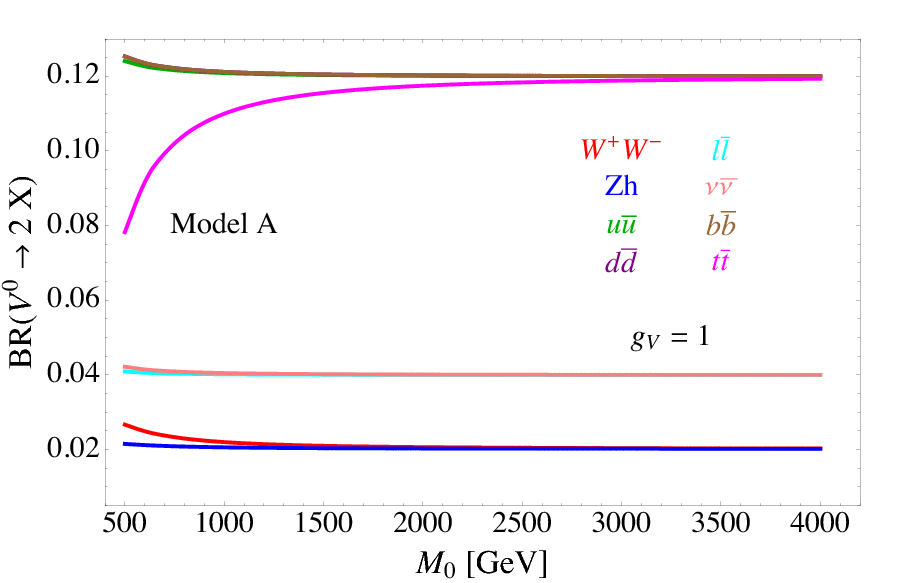
\includegraphics[width=.495\textwidth]{figures/Figures_BRWC.png}%
    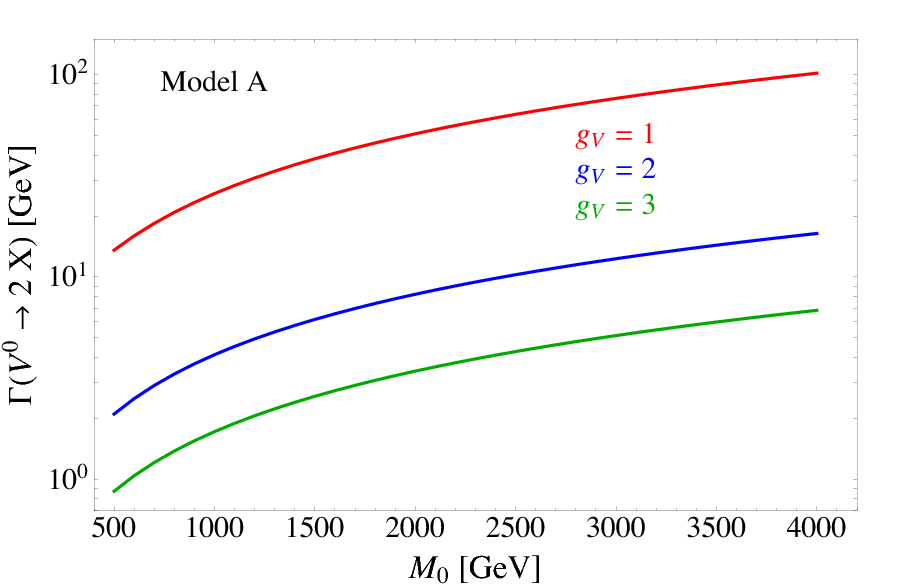
\includegraphics[width=.495\textwidth]{figures/Figures_WidthWC.png}
  \caption{HVT model A scenario: branching fractions for fermionic and bosonic decays when $g_V = 1$ (left) as a function of the mass of the resonance $M_0$; total width of the resonance, as a function of its mass, considering different values of the parameter $g_V$ (right).}
  \label{fig:HVT_modelA_BR_width}
\end{figure}

\subsection{Benchmark model B: strong coupling scenario}
\label{sec:theory_HVT_B}
In composite Higgs models~\cite{Contino2011}, the Higgs boson is the result of the spontaneous symmetry breaking of an $SO(5)$ symmetry to a $SO(4)$ group. New vector bosons are expected to appear, and the lightest ones can be represented by HVT model B when $c_H \sim c_F \sim 1$.\\ 
In this case:
\begin{equation}
\begin{split}
 & g_V c_H \approx -g_V\\
 & g^2 c_F/g_V \approx g^2/g_V,\\
\end{split}
\label{eq:theory_HVT_modelB}
\end{equation}
hence the decay into bosons is not suppressed by $g_V$ parameter. In the benchmark scenario $g_V=3$, decays into dibosons are largely dominant, as it can be seen in fig.~\ref{fig:HVT_modelB_BR_width} (left); the total decay width increases for larger $g_V$ (fig.~\ref{fig:HVT_modelB_BR_width}, right). When the resonances start to be very broad, \textit{i.e.} $\Gamma/M_V \gg 0.1$, the assumptions leading to the simplified model are no longer valid, hence higher order, non-resonant effects must be taken into account.

\begin{figure}[!htb]
  \centering
    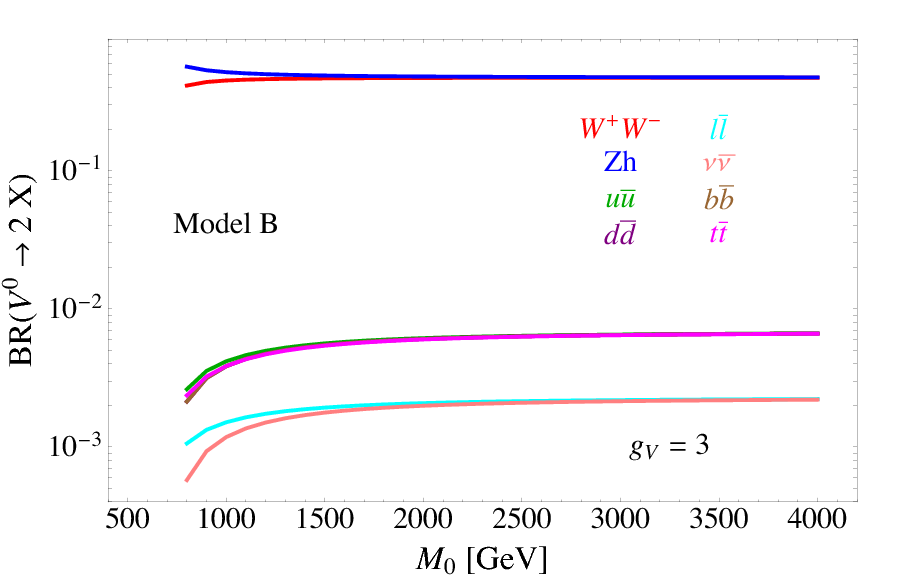
\includegraphics[width=.495\textwidth]{figures/Figures_BRSC.png}%
    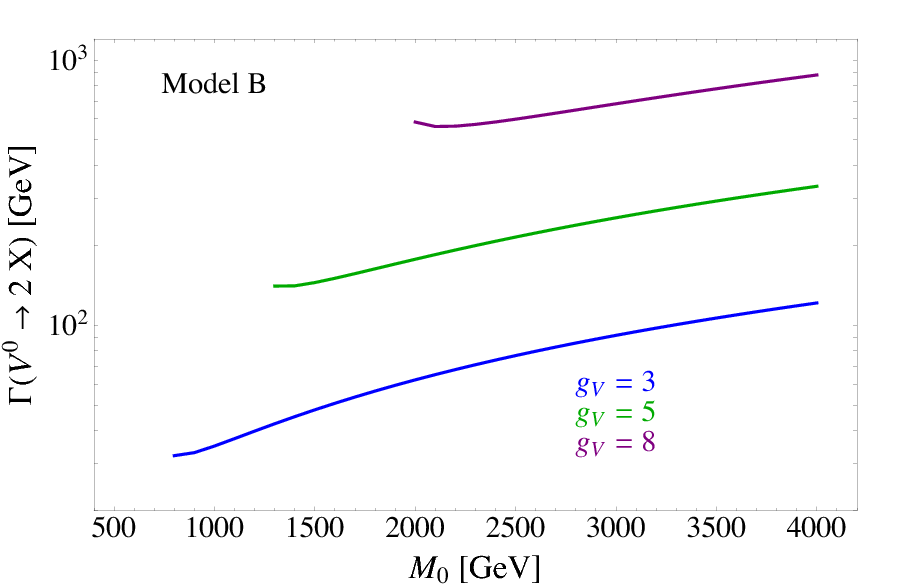
\includegraphics[width=.495\textwidth]{figures/Figures_WidthSC.png}
  \caption{HVT model B scenario: branching fractions for fermionic and bosonic decays when $g_V = 3$ (left) as a function of the mass of the resonance $M_0$; total width of the resonance, as a function of its mass, considering different values of the parameter $g_V$ (right).}
  \label{fig:HVT_modelB_BR_width}
\end{figure}

\subsection{HVT production}
\label{sec:theory_widths}
For resonance masses in the range of interest ($\sim$1 \TeV), the production mechanisms expected to be relevant are Drell-Yan (fig.~\ref{fig:theory_HVT_DY_prod}) and Vector Boson Fusion (VBF) (fig.~\ref{fig:theory_HVT_VBF_prod}).

\begin{figure}[!htb]
  \centering
\feynmandiagram [horizontal=a to b] {
  i1 [particle=\(q\)] -- [fermion] a -- [fermion] i2 [particle=\(\overline{q} \)],
  a -- [red!80!black, boson, edge label=\(V^{0}\), very thick] b,
  f1 [particle=\(\overline{\ell}\)] -- [fermion] b -- [fermion] f2 [particle=\(\ell\)],
};
%
\feynmandiagram [horizontal=a to b] {
  i1 [particle=\(q\)] -- [fermion] a -- [fermion] i2 [particle=\(\overline{q}'\)],
  a -- [red!80!black, boson, edge label=\(V^{-}\), very thick] b,
  f1 [particle=\(Z\)] -- [boson] b -- [boson] f2 [particle=\(W^{-}\)],
};
\caption{Examples of Drell-Yan production mechanism of a heavy $V$ HVT boson: $q$~--~$\bar{q}$ quark scattering producing a neutral $V^{0}$ that decays leptonically (left); $q$~--~$\bar{q}'$ scattering producing a charged $V^{-}$ that decays in a $W$ and $Z$ bosons (right).}
\label{fig:theory_HVT_DY_prod}
\end{figure}

% A bit uglier:
%
%\feynmandiagram [vertical'=a to c, horizontal=b to d] {
%a -- [boson, edge label=\(W^+\)] b,
%b -- [boson, edge label=\(W^-\)] c,
%b -- [red!80!black, boson, edge label=\(V^0\), very thick] d,
%f3 [particle=\(\overline f\)] -- [boson] d -- [boson] f4 [particle=\(f\)],
%
%i1 [particle=\(e^{-}\)]
%-- [fermion] a
%-- [fermion] f1 [particle=\(e^{-}\)],
%
%i2 [particle=\(e^{+}\)]
%-- [fermion] c
%-- [fermion] f2 [particle=\(e^{+}\)],
%};

%\feynmandiagram [vertical'=a to c, horizontal=b to d] {
%i1 [particle=\(e^{-}\)]
%-- [fermion] a
%-- [fermion] f1 [particle=\(e^{-}\)],
%
%i2 [particle=\(e^{+}\)]
%-- [fermion] c
%-- [fermion] f2 [particle=\(e^{+}\)],
%
%a -- [boson, edge label=\(W^+\)] b,
%b -- [boson, edge label=\(W^-\)] c,
%b -- [red!80!black, boson, edge label=\(V^0\), very thick] d,
%
%};
\begin{figure}[!htb]
  \centering
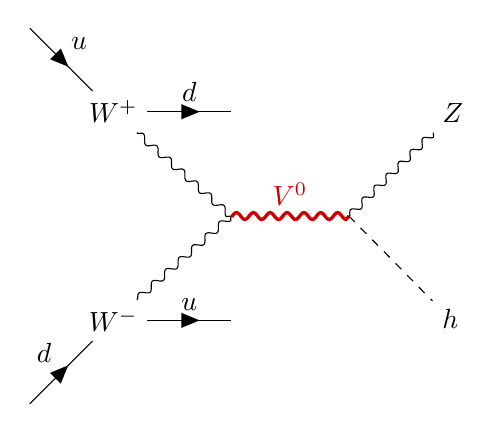
\begin{tikzpicture}
\begin{feynman}
\vertex (e);
\vertex [right=of e] (v); % vertice del bosone V0
\vertex [above right=of v] (m) {\( Z \)};
\vertex [below right=of v] (n) {\( h \)};
\vertex [above left=of e] (c) {\( W^{+} \)};
\vertex [above left=of c] (a);
\vertex [right=of c] (f);

\vertex [below left=of e] (d) {\( W^{-} \)};
\vertex [below left=of d] (b);
\vertex [right=of d] (g);

\diagram* {
(c) -- [boson, edge label'=\(\)] (e), %il bosone collega il vertice (c) col vertice (e) 
(d) -- [boson, edge label=\(\)] (e), %il bosone collega il vertice (d) col vertice (e) W^{-}
(e) -- [red!80!black!, boson, edge label=\(V^0\), very thick] (v), %il bosone collega il vertice (e) col vertice (v)
(v) -- [boson, edge label'=\(\)] (m),
(v) -- [scalar, edge label=\(\)] (n),
(a) -- [fermion, edge label=\(u\)] (c),
(b) -- [fermion, edge label=\(d\)] (d),
(c) -- [fermion, edge label=\(d\)] (f),
(d) -- [fermion, edge label=\(u\)] (g),

};
\end{feynman}
\end{tikzpicture}
\caption{Example of VBF production mechanism of a heavy $V$ HVT boson: a neutral $V^0$ boson is produced by a couple of $W$ bosons, as a result of electroweak interactions of initial state $u$ and $d$ quarks. $V^0$ decays in a $Z$ boson and a Higgs boson. The final state signature includes the presence of a pair of quarks, due to the primary interactions.}
\label{fig:theory_HVT_VBF_prod}
\end{figure}

\noindent The cross-section of the production mechanisms is given by:
\begin{equation}
\sigma (pp \rightarrow V + X) = \left. \sum_{i, j \in p} \frac{\Gamma_{V \rightarrow ij}}{M_V} f(J, S_i, S_j) g(C_i, C_j) \frac{dL_{ij}}{ds} \right|_{s = M_V^2},
\label{eq:prod_xsec}
\end{equation}
where $i$, $j$ are the partons involved in the hard interaction, $\Gamma_{V \rightarrow ij}$ is the partial width of the process $V \rightarrow ij$, $f(J, S_i, S_j)$ is a function of the spin of the resonance and of the partons, $g(C_i, C_j)$ is a function of the colour factors of each parton, $s$ is the center-of-mass energy and $\frac{dL_{ij}}{ds}$ are the parton luminosities, that are independent from HVT model (that enters only in $\Gamma_{ij}$).
\\
Parton luminosities, calculated for a center-of-mass energy of 14 TeV starting from quark and antiquark parton distribution functions (PDF), are displayed in fig.~\ref{fig:HVT_DY_partolumi} (Drell-Yan mechanism) and~\ref{fig:HVT_VBF_partolumi} (VBF mechanism). VBF luminosities are suppressed by the $\alpha_{\text{weak}}$ factor, therefore the process is relevant only when the bosonic decays of the triplet are dominant (strongly coupled scenario). 
\begin{figure}[!htb]
  \centering
    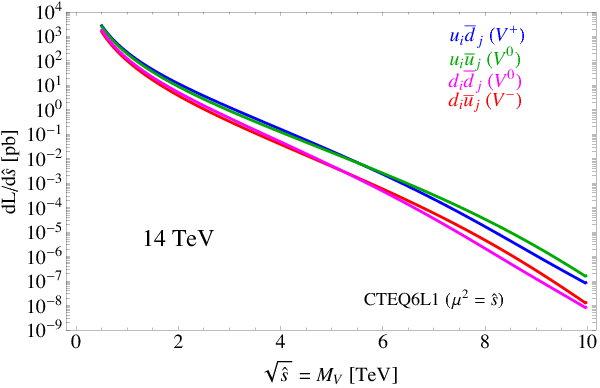
\includegraphics[width=.495\textwidth]{figures/Figures_LumiDY14.png}
  \caption{Parton luminosities for Drell-Yan process between $i$ and $j$ partons, as a function of the parton center-of-mass energy, for the LHC proton-proton collisions performed at 14 TeV.}
  \label{fig:HVT_DY_partolumi}
\end{figure}

\begin{figure}[!htb]
  \centering
    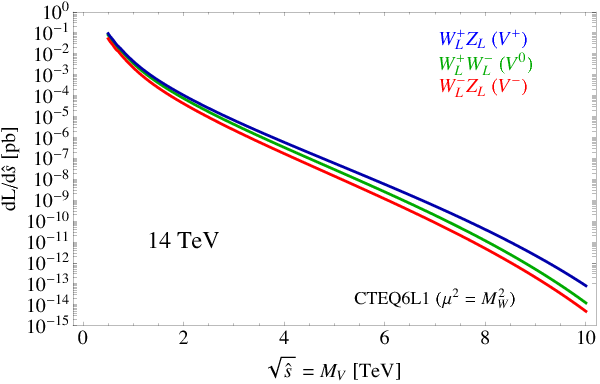
\includegraphics[width=.495\textwidth]{figures/Figures_LumiVBF14.png}
  \caption{Parton luminosities for VBF process between $i$ and $j$ partons, as a function of the parton center-of-mass energy, for the LHC proton-proton collisions performed at 14 TeV.}
  \label{fig:HVT_VBF_partolumi}
\end{figure}

\clearpage

\subsection{Search for HVT resonances at LHC}
\label{sec:theory_HVT_limits_LHC}
No evidence of HVT resonances has been observed so far at LHC experiments. Data collected by ATLAS and CMS detectors are used to set limits on the HVT resonance masses and coupling parameters. Experimental results from proton-proton collisions performed at a center-of-mass energy of 8 TeV (Run 1 era) at LHC brought to the following conclusions. A weakly coupled resonance, in the context of benchmark model A ($g_V = 1$) was excluded up to 3 TeV by Run 1 data. By looking at parton luminosities in fig.\ref{fig:HVT_DY_partolumi}, in data produced by LHC proton-proton collision at 14 TeV, collected for an integrated luminosity of 300 $\mbox{fb}^{-1}$, the sensitivity is expected to increase up to $m_V \approx 6$ TeV. A strongly coupled resonance, in the context of benchmark model B ($g_V = 3$) is excluded up to 2 TeV by Run 1 data. Data produced by LHC at 14 TeV should increase the sensitivity up to $m_V \approx 3-4$ TeV.\\
The most stringent limits are provided by the latest data produced by LHC at a center-of-mass energy of 13 TeV (Run 2 era).

\vspace*{1\baselineskip}

\noindent Numerous searches for HVT triplet have been performed at CMS experiment in different final states: the most sensitive ones were those in all-hadronic topology. \cite{Sirunyan:2017acf,bib:CMS-PAS-B2G-17-001} (search for $WW$, $WZ$, $ZZ$ resonances in the $q\bar{q}q\bar{q}$ final state) excludes a $W'$ with mass below 3.6 and a $Z'$ with mass below 2.7 TeV in the model B scenario (fig.~\ref{fig:theory_B2G-17-001}). \cite{CMS:2017eme,bib:CMS-PAS-B2G-17-002} (search for $WH$, $ZH$ resonances in the $q\bar{q} b \bar{b}$ final state) excludes a $W'$ lighter than 2.97 (3.15) TeV in the HVT model A (model B), and a $Z'$ up to 1.67 (2.26) TeV in HVT model A (model B) (fig.~\ref{fig:theory_B2G-17-002}). In fig.~\ref{fig:theory_exclusion_parameter_plane}, results of \cite{Sirunyan:2017acf,bib:CMS-PAS-B2G-17-001} (left) and \cite{CMS:2017eme,bib:CMS-PAS-B2G-17-002} (right) searches are interpreted as exclusion contours in the coupling parameter plane of the HVT model ($g_Vc_H$ and $g^2 c_F/g_V$). In the grey shaded area, the narrow width approximation fails. The colored curves display the parameter exclusion for different mass hypoteses of the triplet. Colored dots show the model A and B benchmark scenarios.

\begin{figure}[!htb]
  \centering
    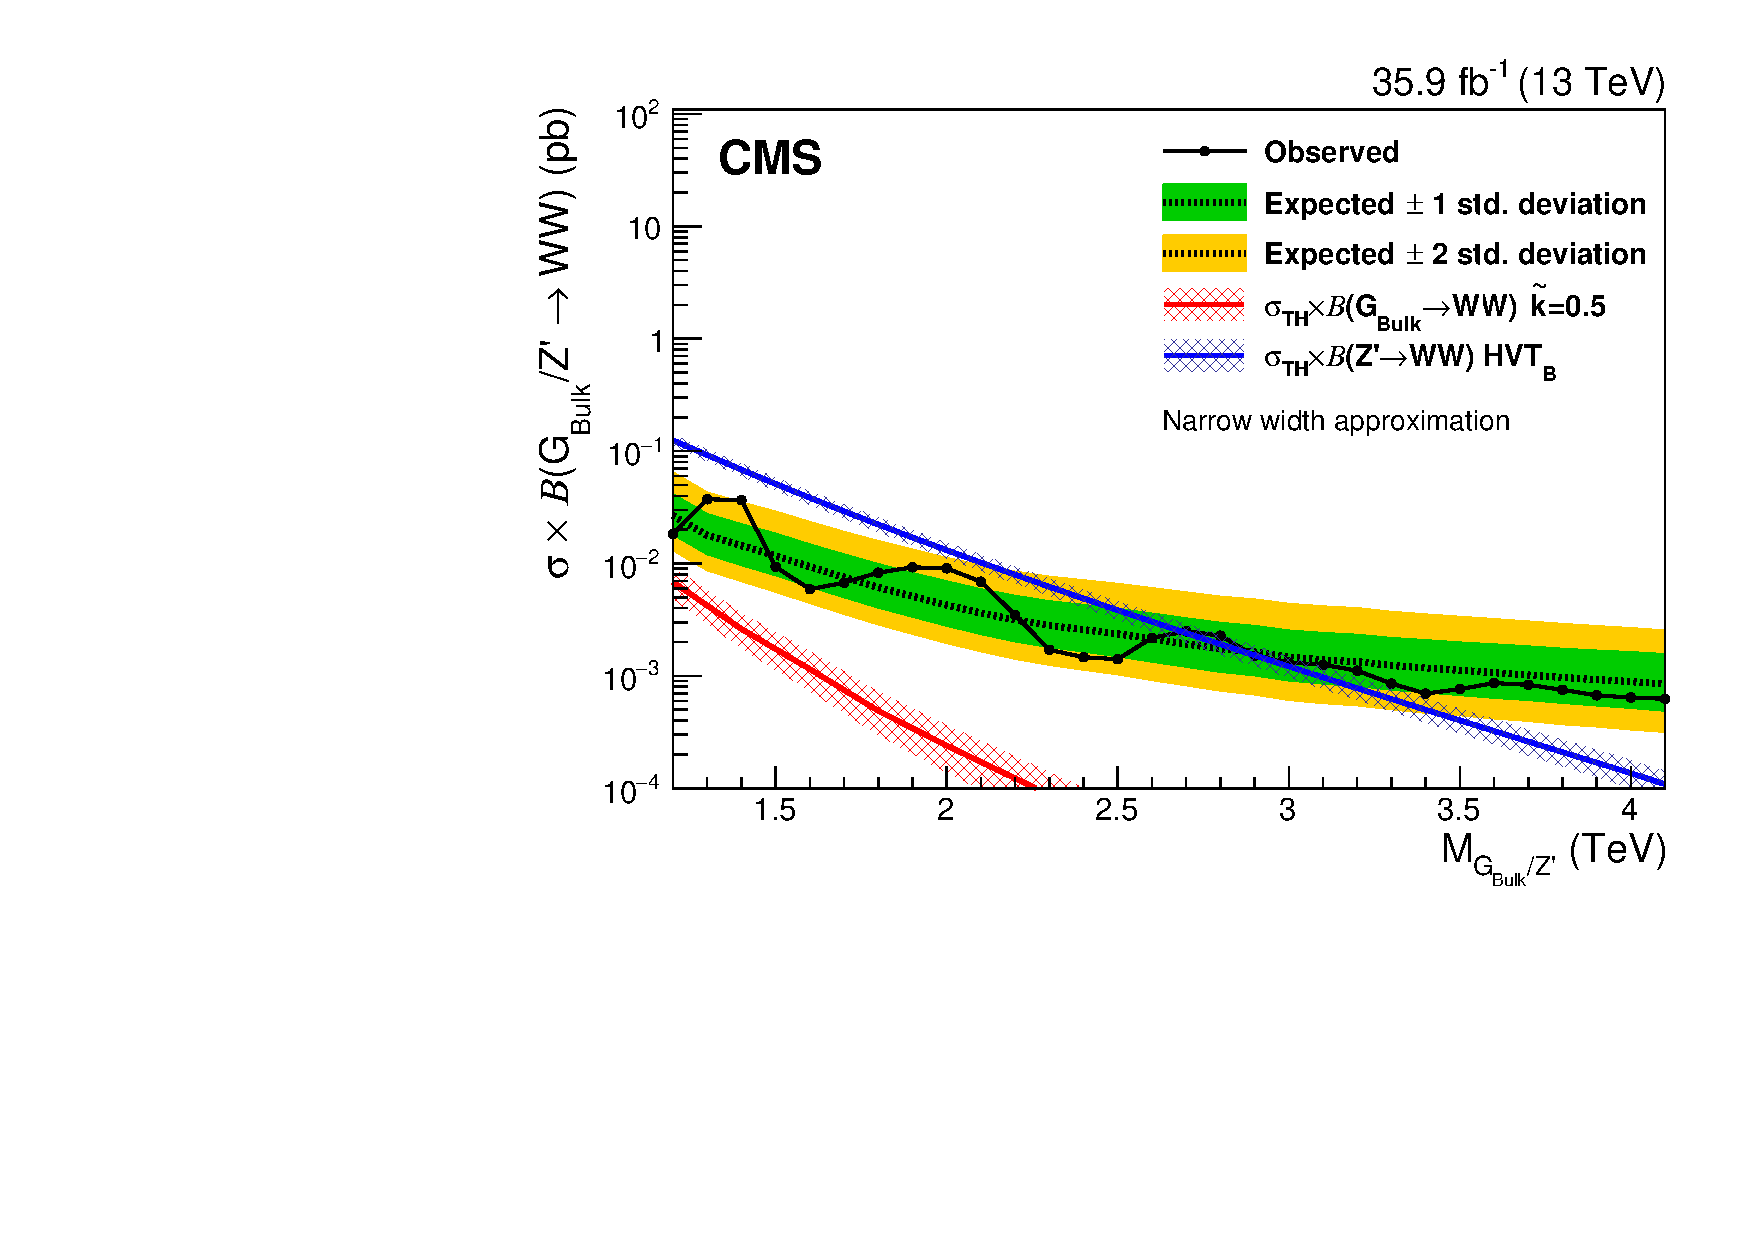
\includegraphics[width=.495\textwidth]{figures/B2G-17-001/CMS-B2G-17-001_Figure_006-a.pdf}%
    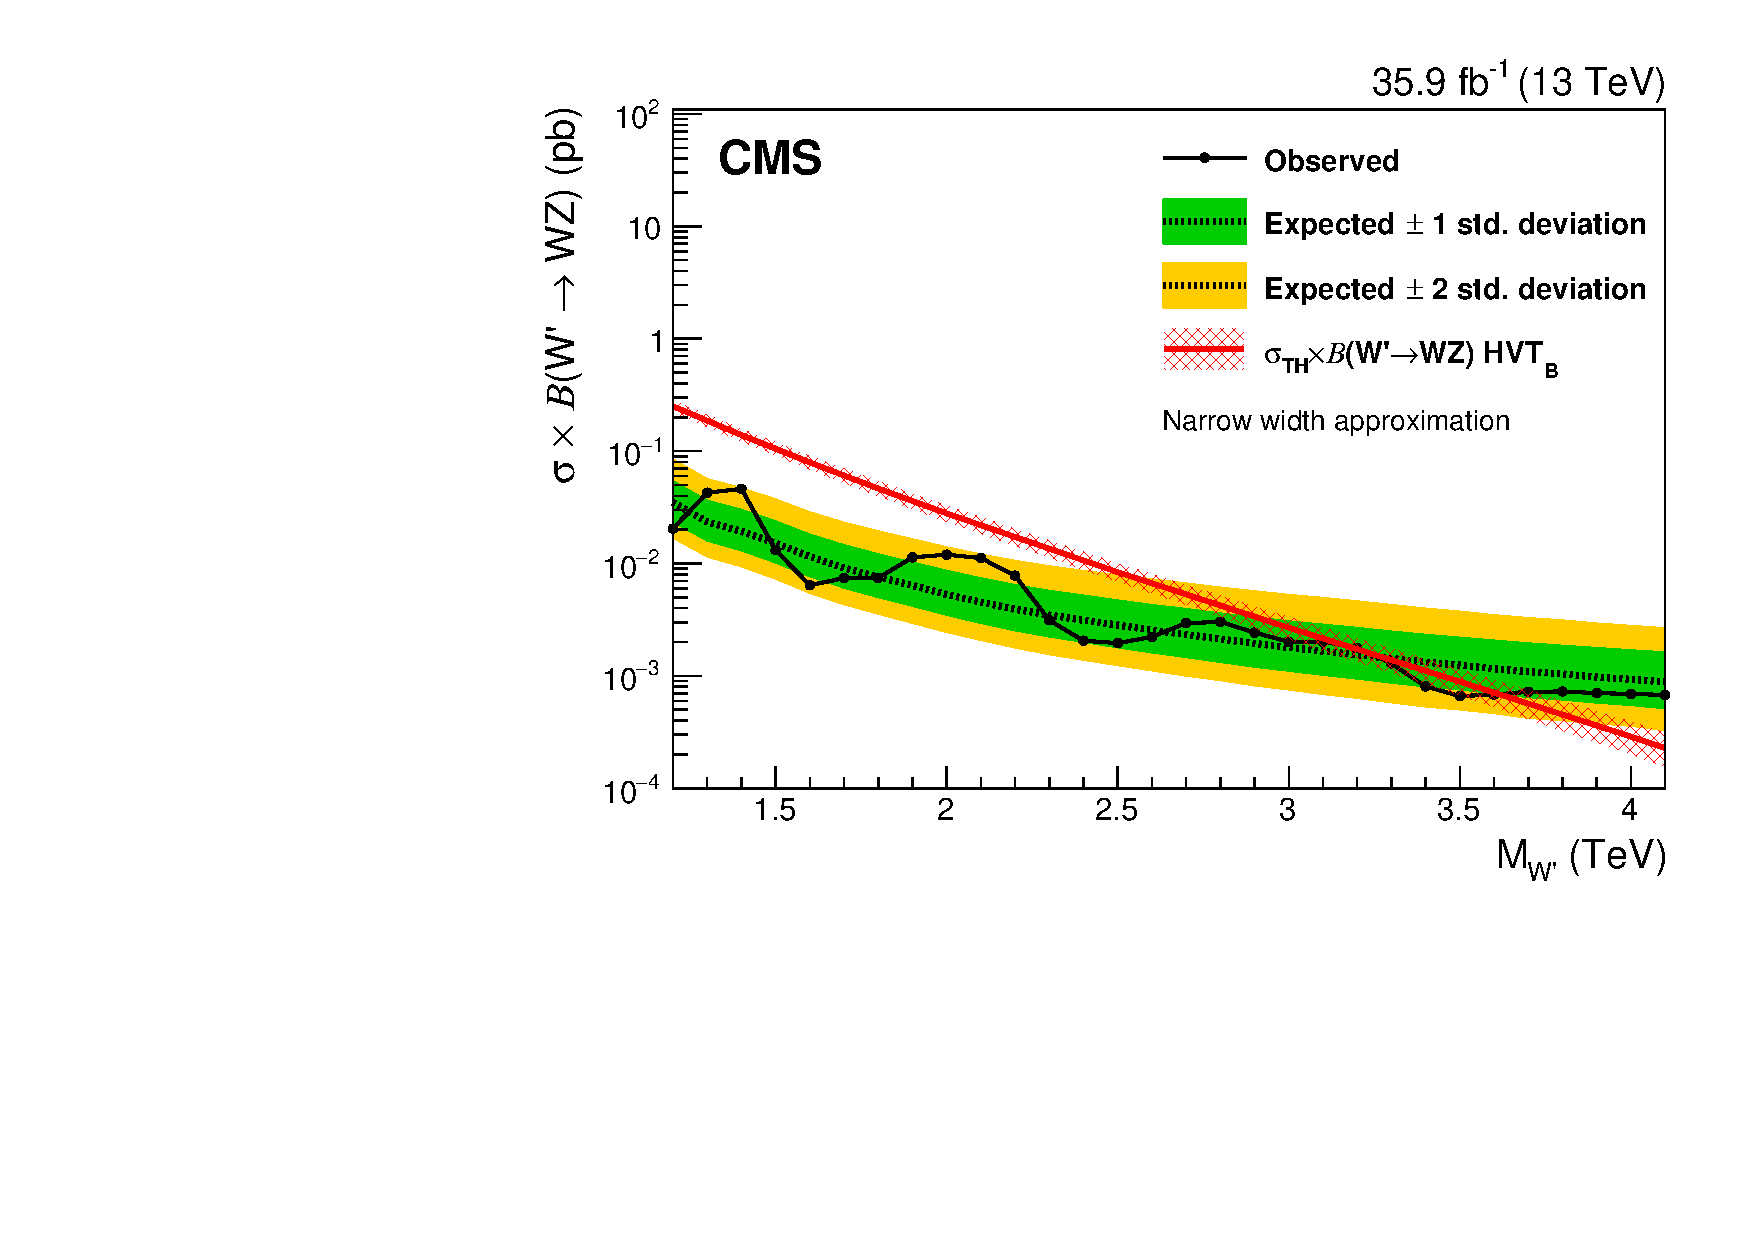
\includegraphics[width=.495\textwidth]{figures/B2G-17-001/CMS-B2G-17-001_Figure_006-b.pdf}
  \caption{The observed and expected limits, with 68\% and 95\% uncertainty bands, on the product of the cross-section and branching fraction $\sigma \mathcal{B} (Z' \rightarrow WW)$ for a spin-1 $Z'$ (left) and $\sigma \mathcal{B} (W' \rightarrow WZ)$ for a spin-1 $W'$ (right), as a function of the reconstructed mass of the diboson resonance. The colored lines show the theoretical predictions for the HVT model B.}
  \label{fig:theory_B2G-17-001}
\end{figure}

\begin{figure}[!htb]
  \centering
    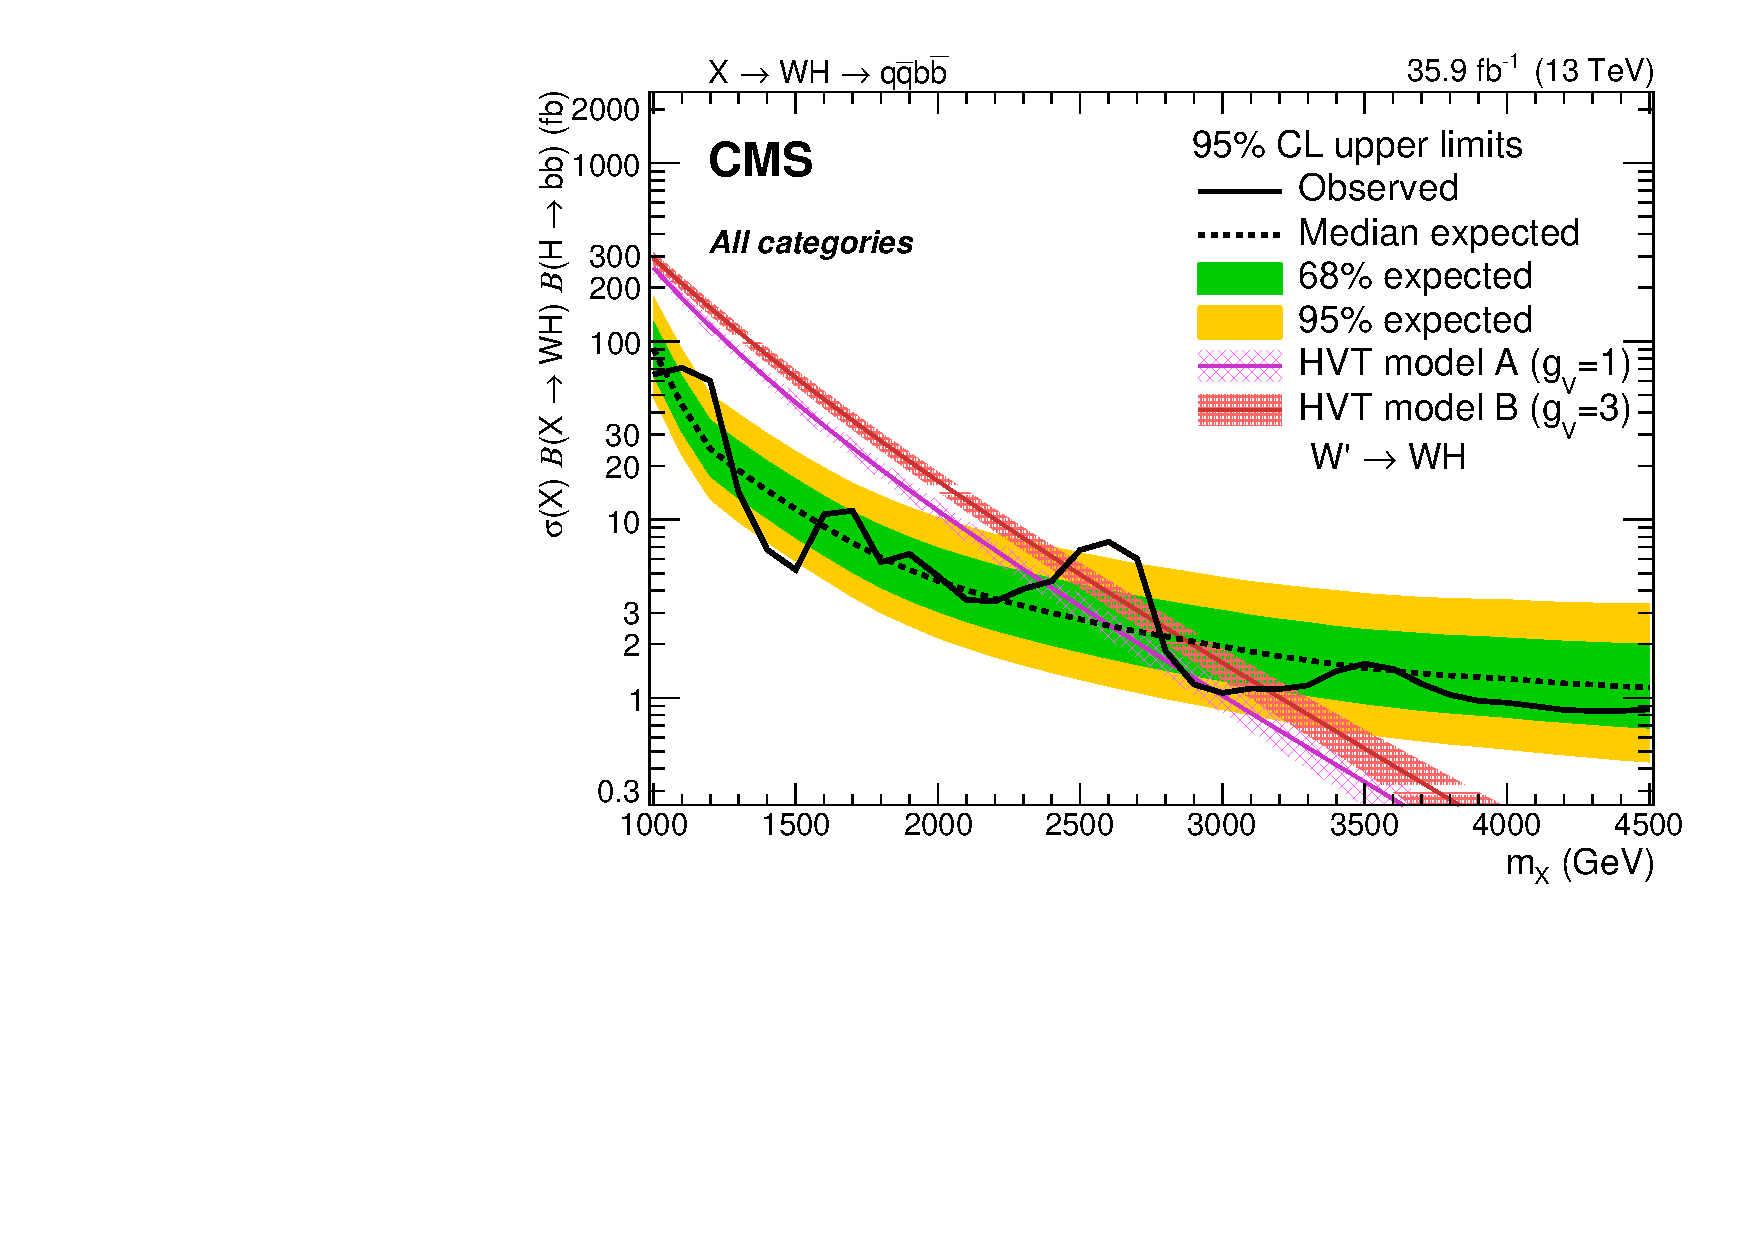
\includegraphics[width=.495\textwidth]{figures/B2G-17-002/CMS-B2G-17-002_Figure_005-a.pdf}%
    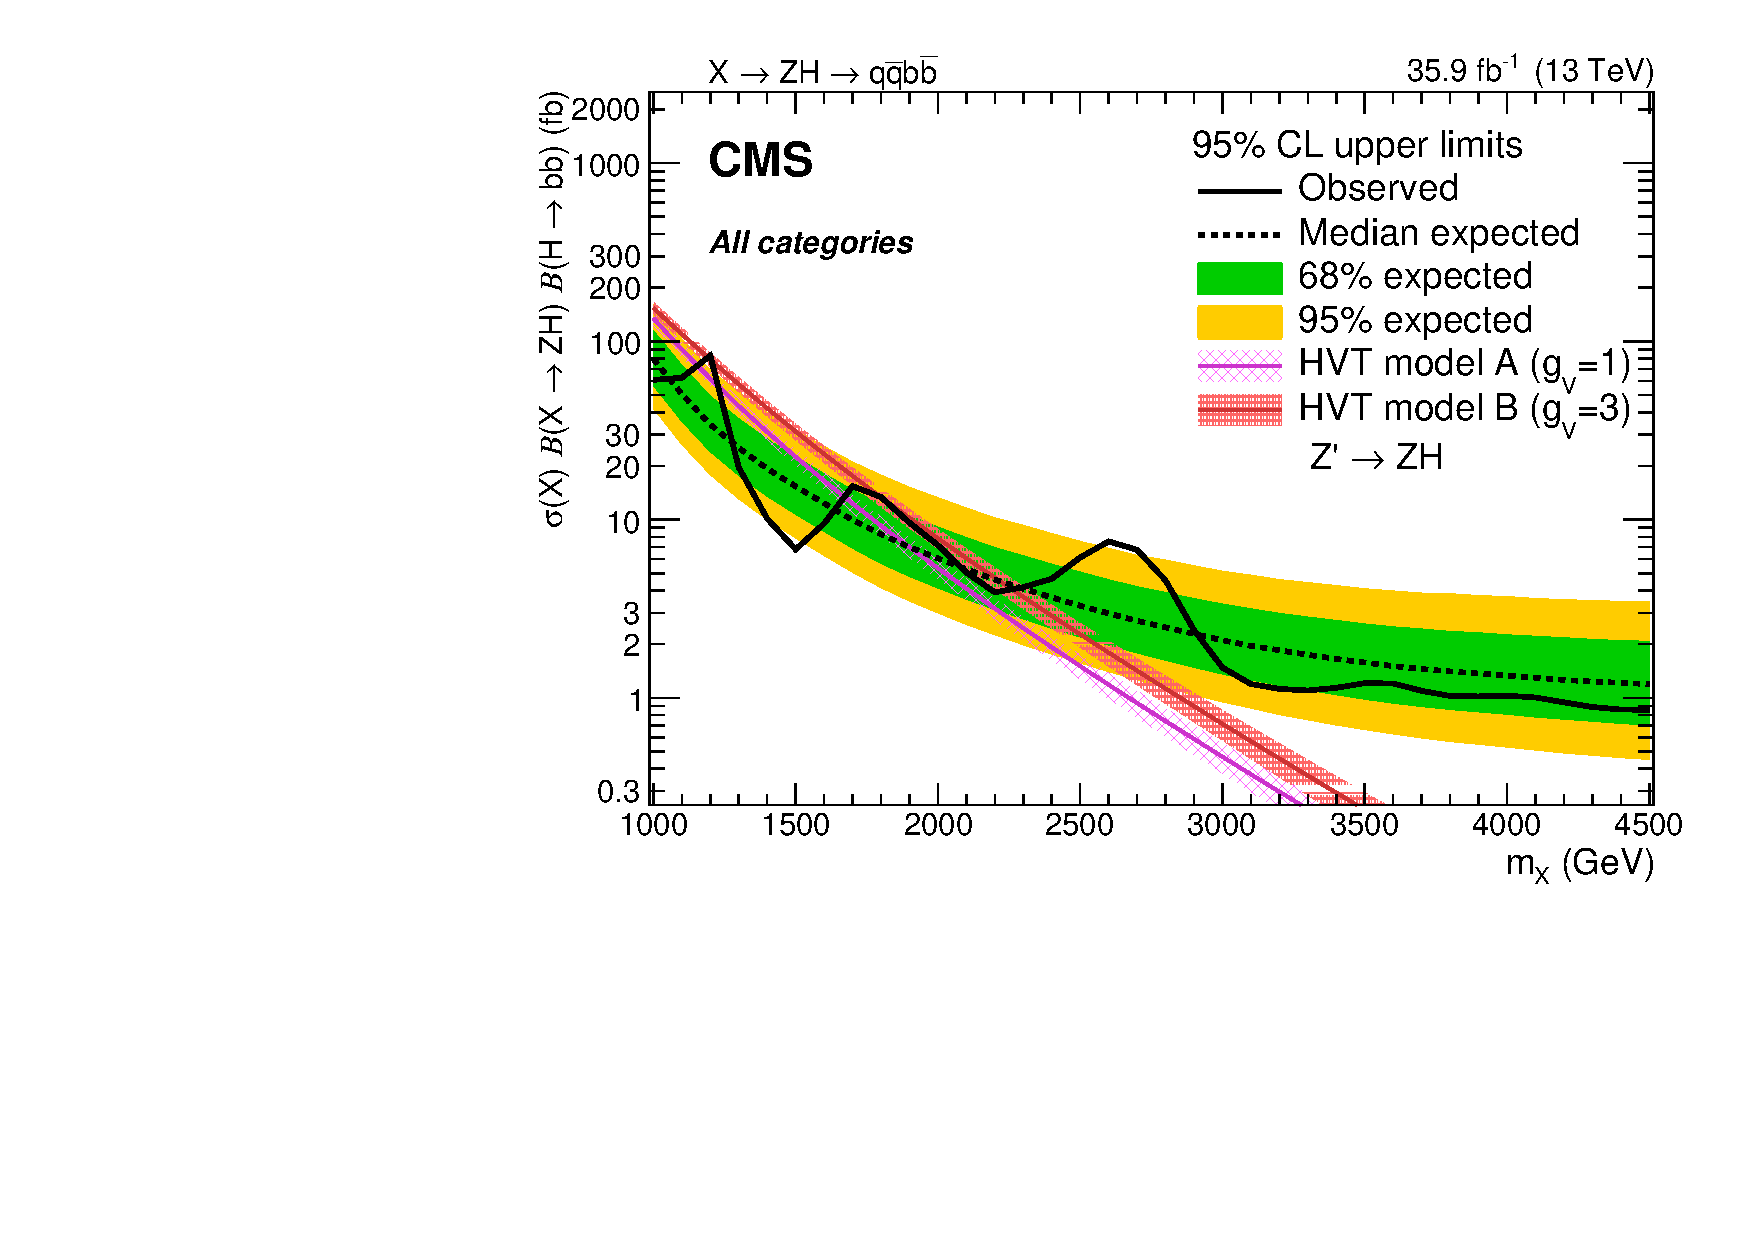
\includegraphics[width=.495\textwidth]{figures/B2G-17-002/CMS-B2G-17-002_Figure_005-b.pdf}
  \caption{The observed and expected limits, with 68\% and 95\% uncertainty bands, on the product of the cross-section and branching fraction $\sigma \mathcal{B} (W' \rightarrow WH)$ for a spin-1 $W'$ (left) and $\sigma \mathcal{B} (Z' \rightarrow ZH)$ for a spin-1 $Z'$ (right), as a function of the reconstructed mass of the diboson resonance. The colored lines show the theoretical predictions for the HVT model A and B.}
  \label{fig:theory_B2G-17-002}
\end{figure}

\begin{figure}[!htb]
  \centering
    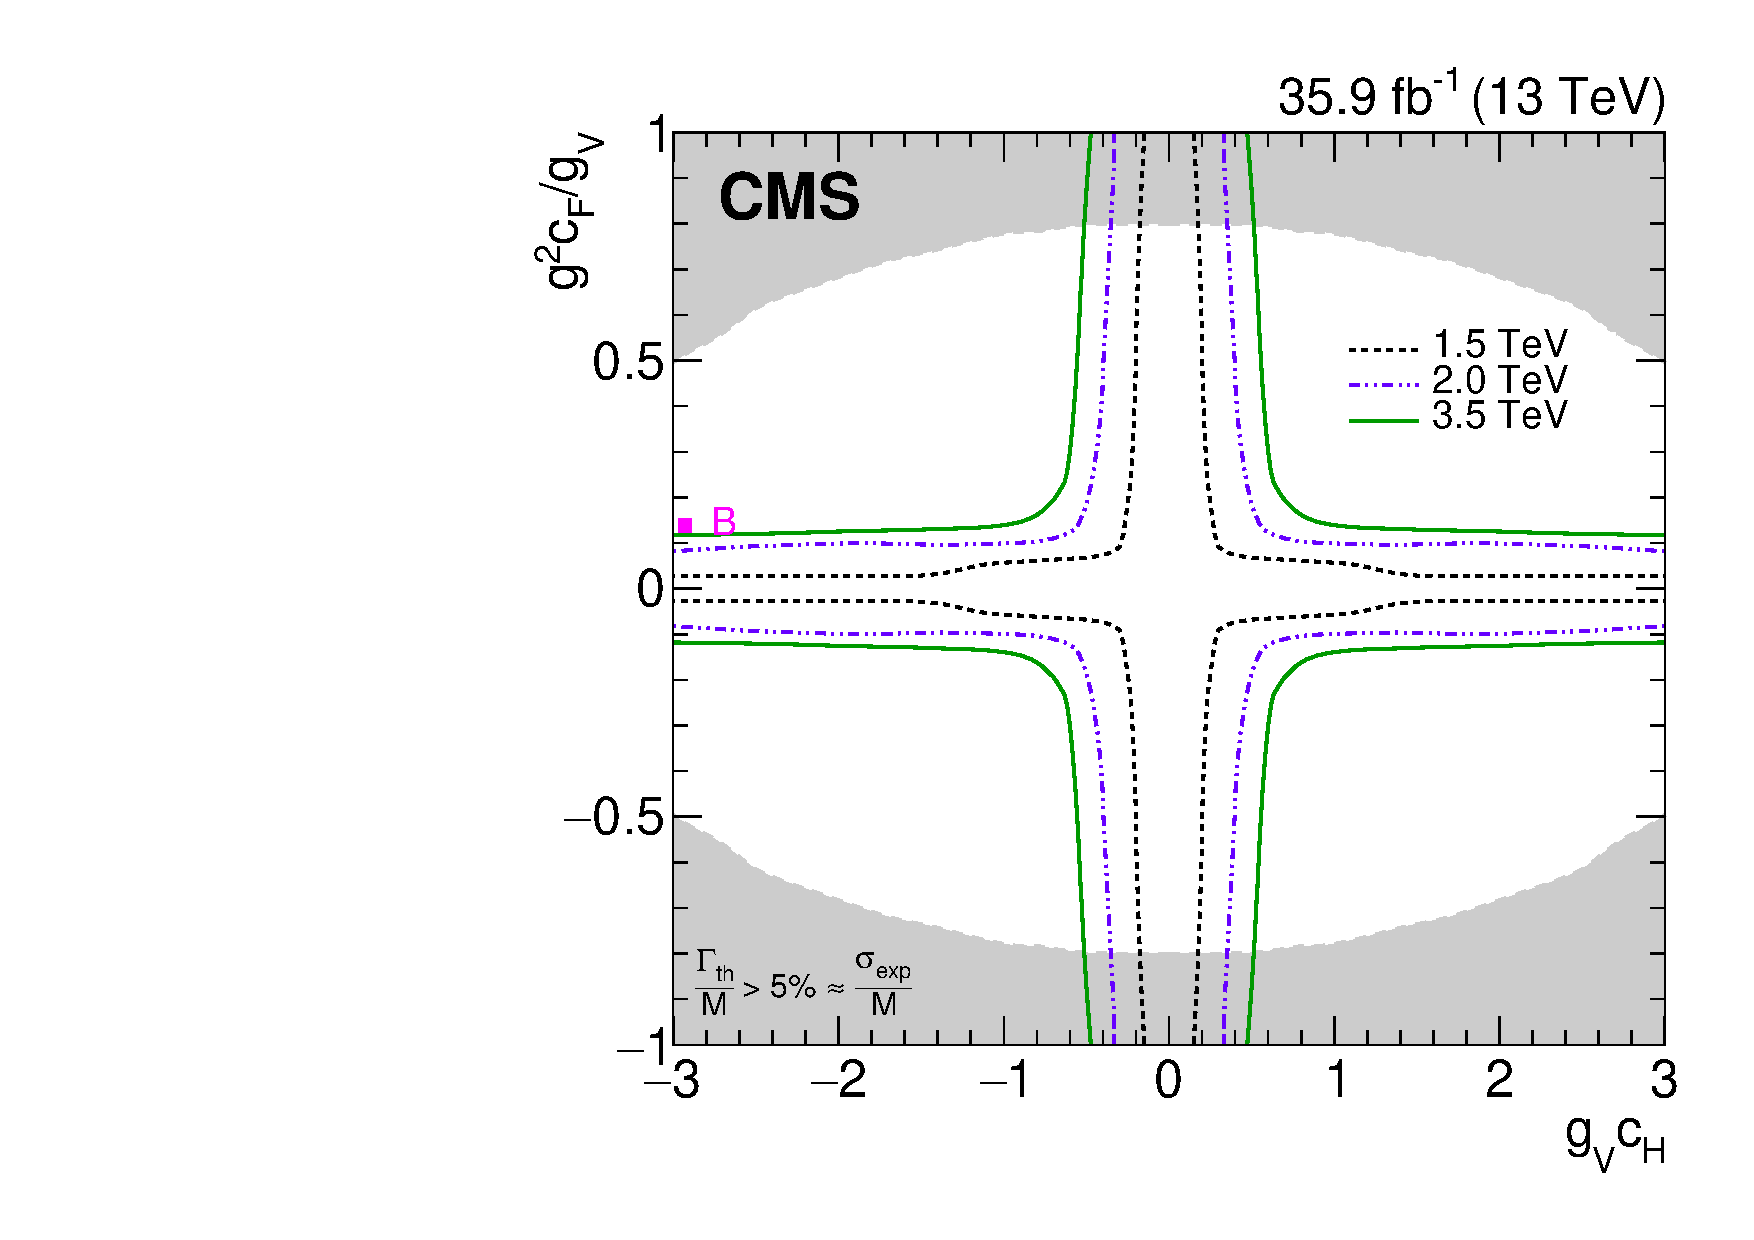
\includegraphics[height=.4\textwidth]{figures/B2G-17-001/CMS-B2G-17-001_Figure_007.pdf}%
    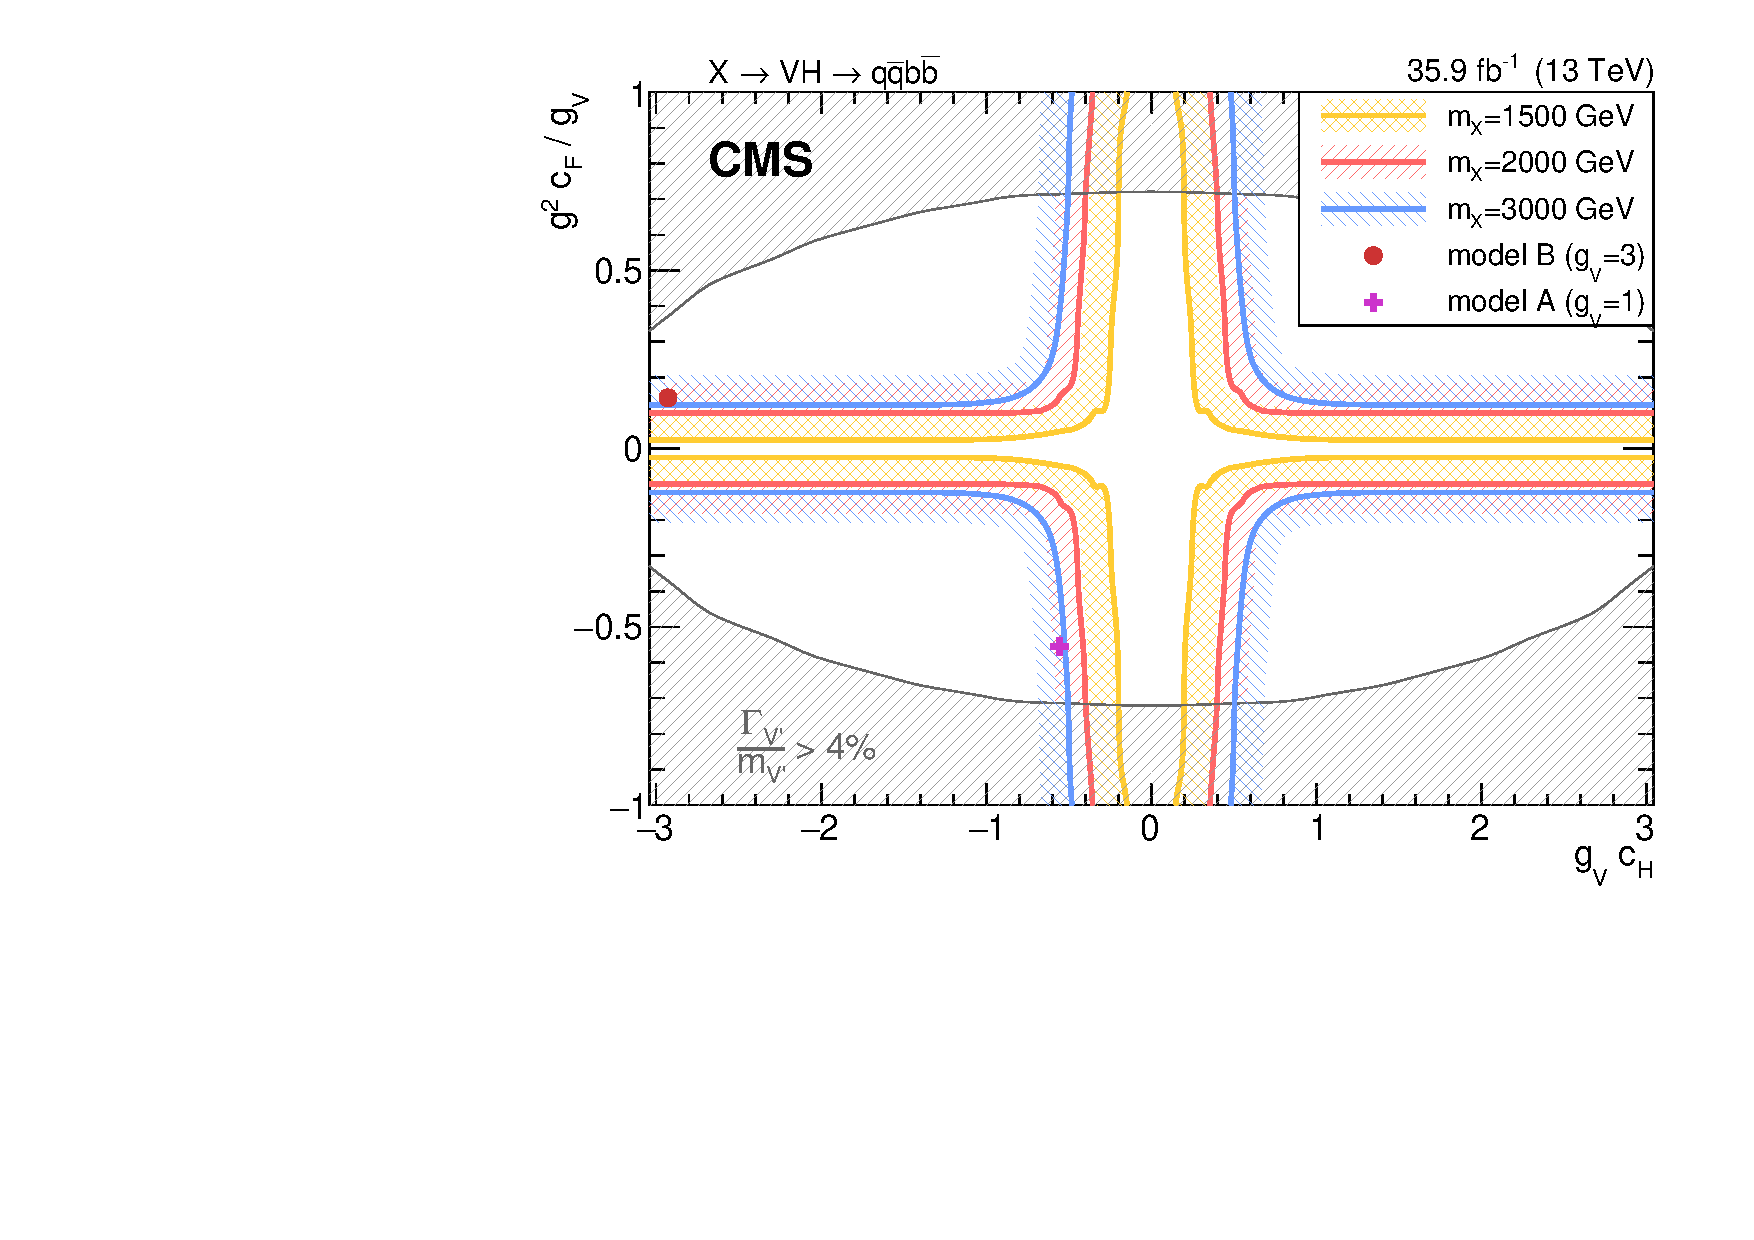
\includegraphics[height=.4\textwidth]{figures/B2G-17-002/CMS-B2G-17-002_Figure_007.pdf}
  \caption{Exclusion contours in the coupling parameter plane of the HVT model ($g_Vc_H$ and $g^2 c_F/g_V$).}
  \label{fig:theory_exclusion_parameter_plane}
\end{figure}

\clearpage

\noindent Many other final states have been exploited at CMS: $ZW, ZZ \rightarrow \ell \bar{\ell} q\bar{q}$~\cite{CMS-PAS-B2G-16-022}; $WH, ZH \rightarrow (\ell \bar{\ell}, \ell \nu, \nu \bar{\nu}) b \bar{b}$~\cite{Khachatryan:2016cfx}; $WZ, WW \rightarrow \ell \nu q \bar{q}$~\cite{CMS-PAS-B2G-16-020}. Finally, $ZW, ZZ \rightarrow \nu \bar{\nu} q \bar{q}$~\cite{CMS-PAS-B2G-17-005} results will be extensively described in this thesis. 

\vspace*{1\baselineskip}

%Revision
%
\noindent The results (or preliminary results) on HVT searches in diboson final states, performed with 2016 data and published by the CMS Collaboration so far, are summarized in fig.~\ref{fig:theory_CMS_Diboson_Summary_HVT}. The dark orange curve corresponds to the $(WZ, WW) \rightarrow q\bar{q}q\bar{q}$ analysis~\cite{Sirunyan:2017acf,bib:CMS-PAS-B2G-17-001}; the light blue curve corresponds to the $(WH, ZH) \rightarrow q\bar{q} b \bar{b}$ analysis~\cite{CMS:2017eme,bib:CMS-PAS-B2G-17-002}; the light orange curve corresponds to the analysis discussed in this thesis~\cite{CMS-PAS-B2G-17-005}.

\begin{figure}[!htb]
  \centering
    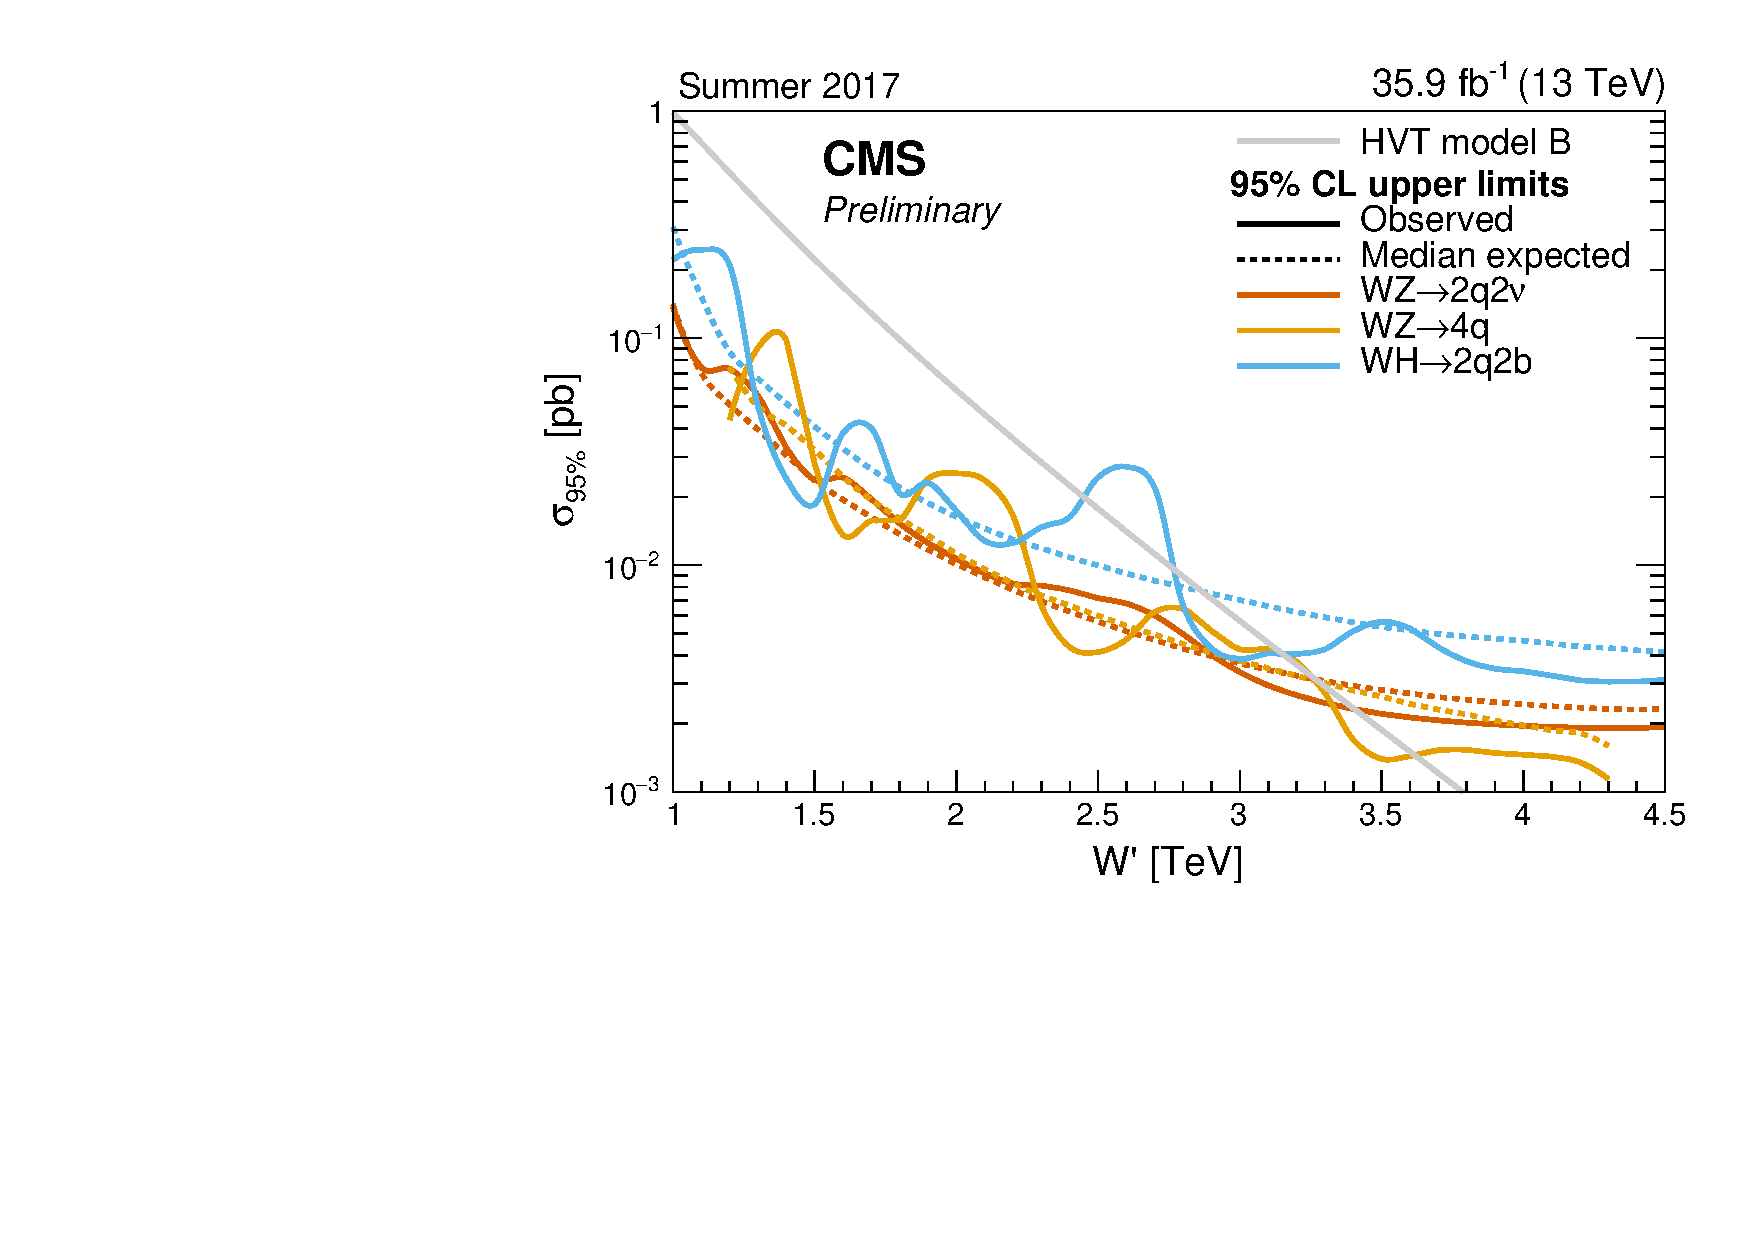
\includegraphics[width=.495\textwidth]{figures/combiLimitsWprime_HVTB.pdf}%
    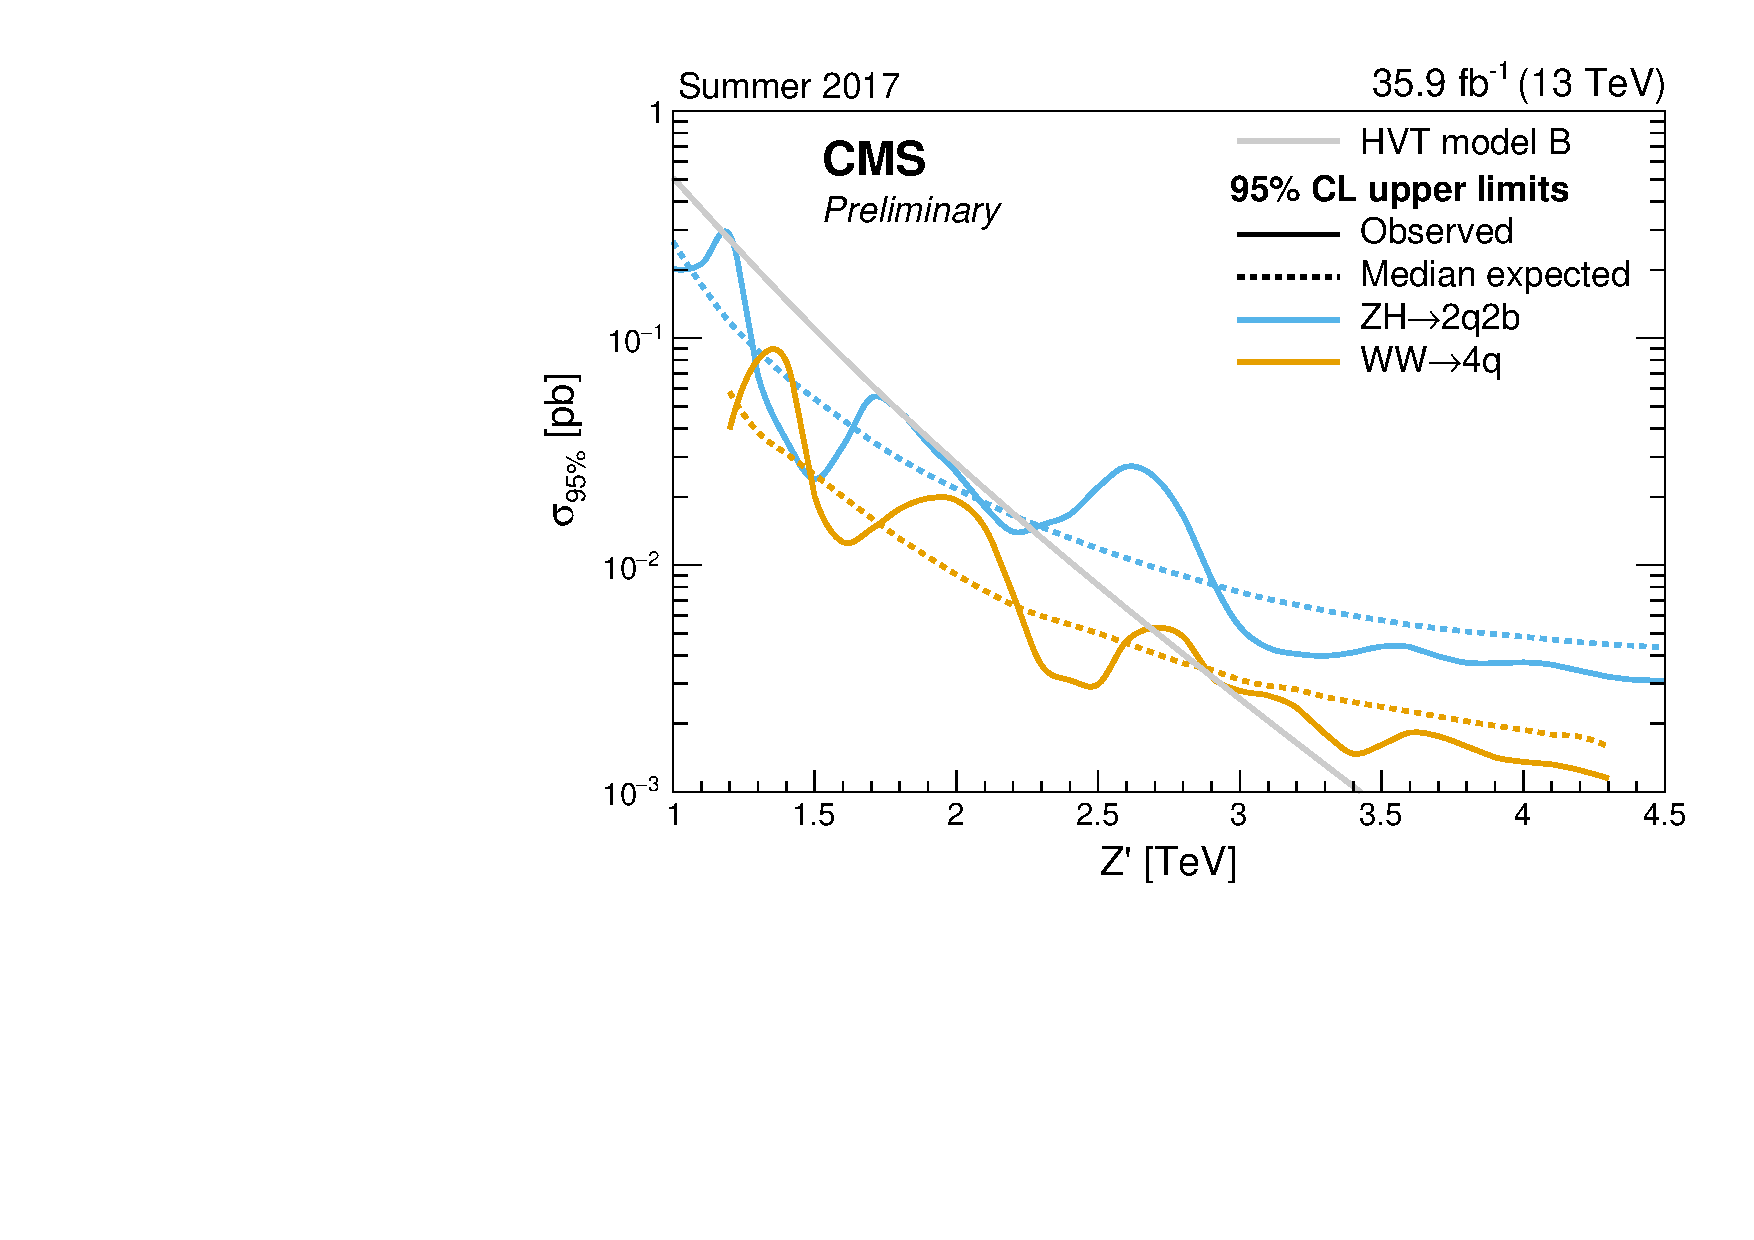
\includegraphics[width=.495\textwidth]{figures/combiLimitsZprime_HVTB.pdf}
  \caption{The observed and expected limits on the product of the cross-section and branching fraction $\sigma \mathcal{B} (W' \rightarrow (WZ, WH))$ for a spin-1 $W'$ (left) and $\sigma \mathcal{B} (Z' \rightarrow (ZH, WW))$ for a spin-1 $Z'$ (right), as a function of the reconstructed mass of the diboson resonance. The gray line show the theoretical prediction for the HVT model B.}
  \label{fig:theory_CMS_Diboson_Summary_HVT}
\end{figure}


%\clearpage

\noindent Searches for HVT model B resonances have been performed at ATLAS experiment as well. Results for a $W' \rightarrow WZ$ reported in fig.~\ref{fig:theory_ATLAS_Diboson_Summary} include the searches performed in $WW, WZ, ZZ \rightarrow q \bar{q} q \bar{q}$ final state~\cite{Aaboud:2017eta}; $WZ, WW \rightarrow \ell \nu q \bar{q}$ final state~\cite{ATLAS-CONF-2017-051}; $ZW, ZZ \rightarrow (\ell \bar{\ell}, \ell \nu, \nu \bar{\nu}) q \bar{q}$ final state~\cite{ATLAS-CONF-2016-082}. The all-hadronic final state has the best sensitivity and it excludes a $W'$ resonance up to 3.3 TeV (model B scenario). Results for a $W' \rightarrow WH$ and for a $Z' \rightarrow ZH$ are displayed in fig.~\ref{fig:theory_ATLAS_Diboson_Summary_VH} (left and right respectively), and they include searches performed in $WH, ZH \rightarrow q \bar{q} b \bar{b}$ final state~\cite{Aaboud:2017ahz}, and $WH, ZH \rightarrow \ell \bar{\ell}, \ell \nu, \nu \bar{\nu}) b \bar{b}$~\cite{ATLAS-CONF-2017-055}. A $W'$ is excluded up to 2.9 TeV and a $Z'$ is excluded up to 2.8 TeV (in the model B scenario).

\begin{figure}[!htb]
  \centering
    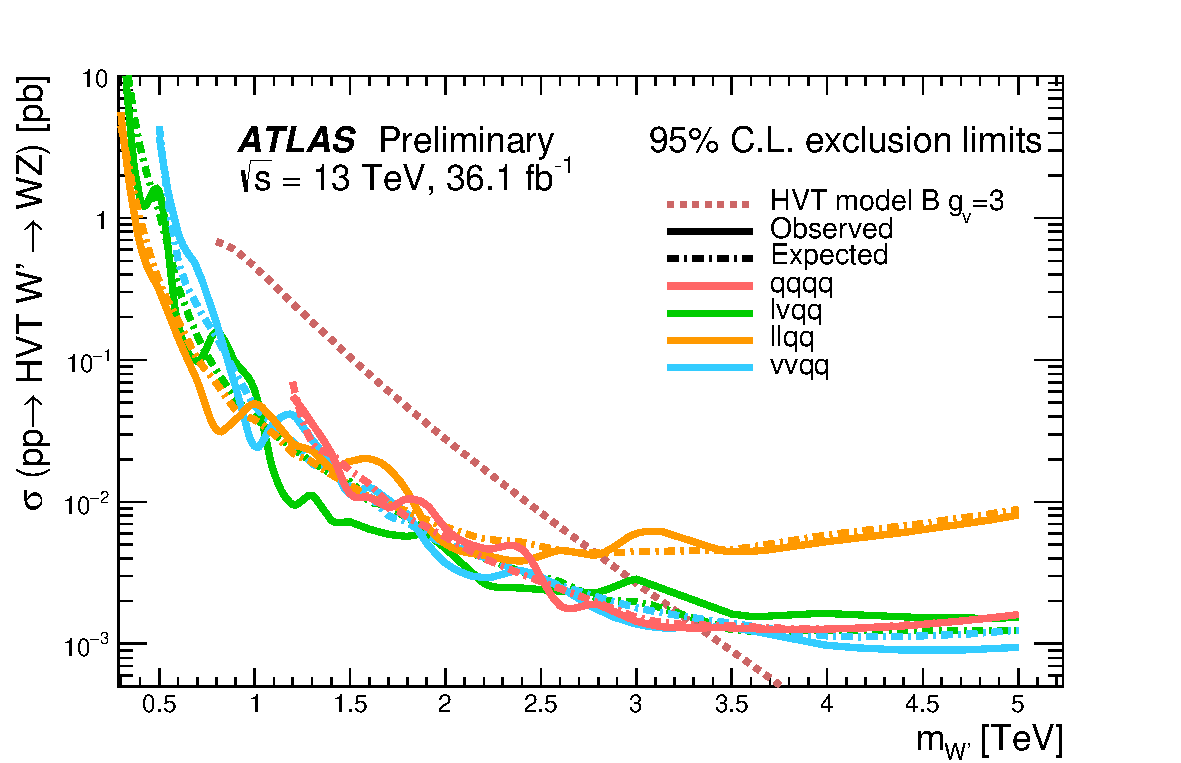
\includegraphics[width=.495\textwidth]{figures/ATLAS_Diboson_Summary.pdf}
  \caption{The observed and expected limits on the product of the cross-section and branching fraction $\sigma \mathcal{B} (W' \rightarrow WZ)$ for a spin-1 $W'$, as a function of the reconstructed mass of the diboson resonance. The dotted line shows the theoretical predictions for the HVT model B.}
  \label{fig:theory_ATLAS_Diboson_Summary}
\end{figure}

\begin{figure}[!htb]
  \centering
    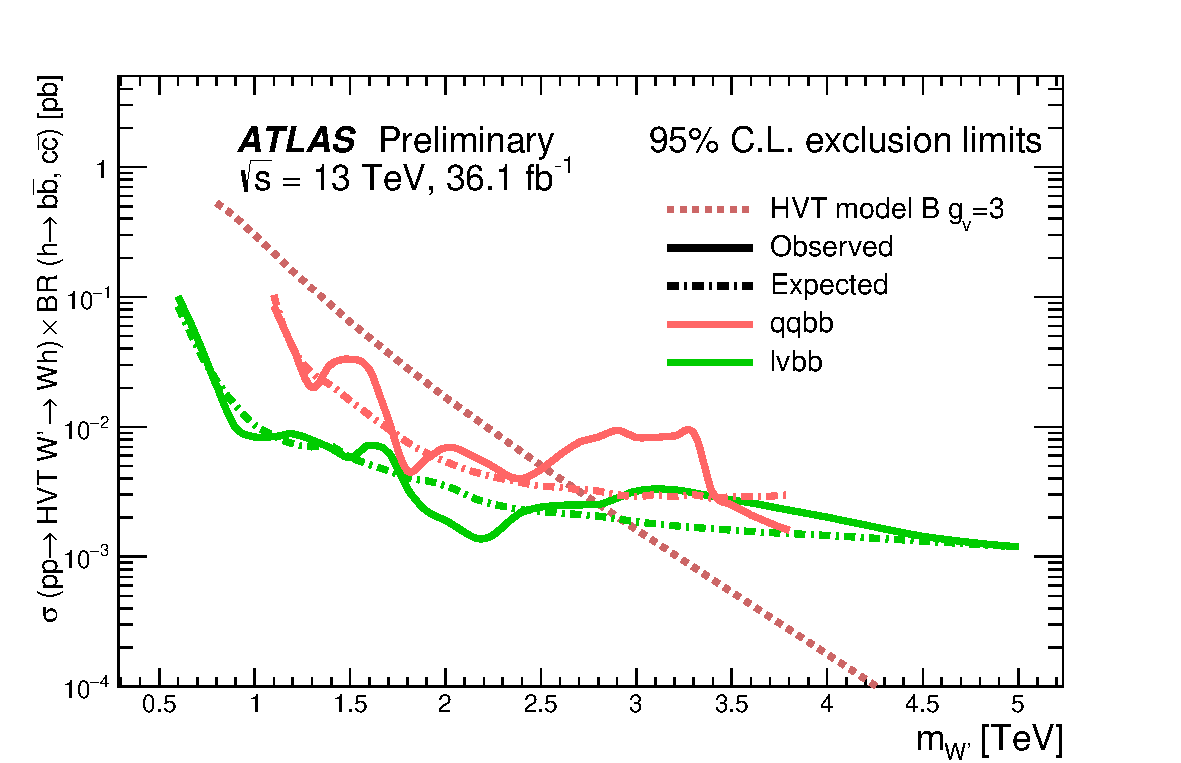
\includegraphics[width=.495\textwidth]{figures/ATLAS_Diboson_Summary_VH.pdf}%
    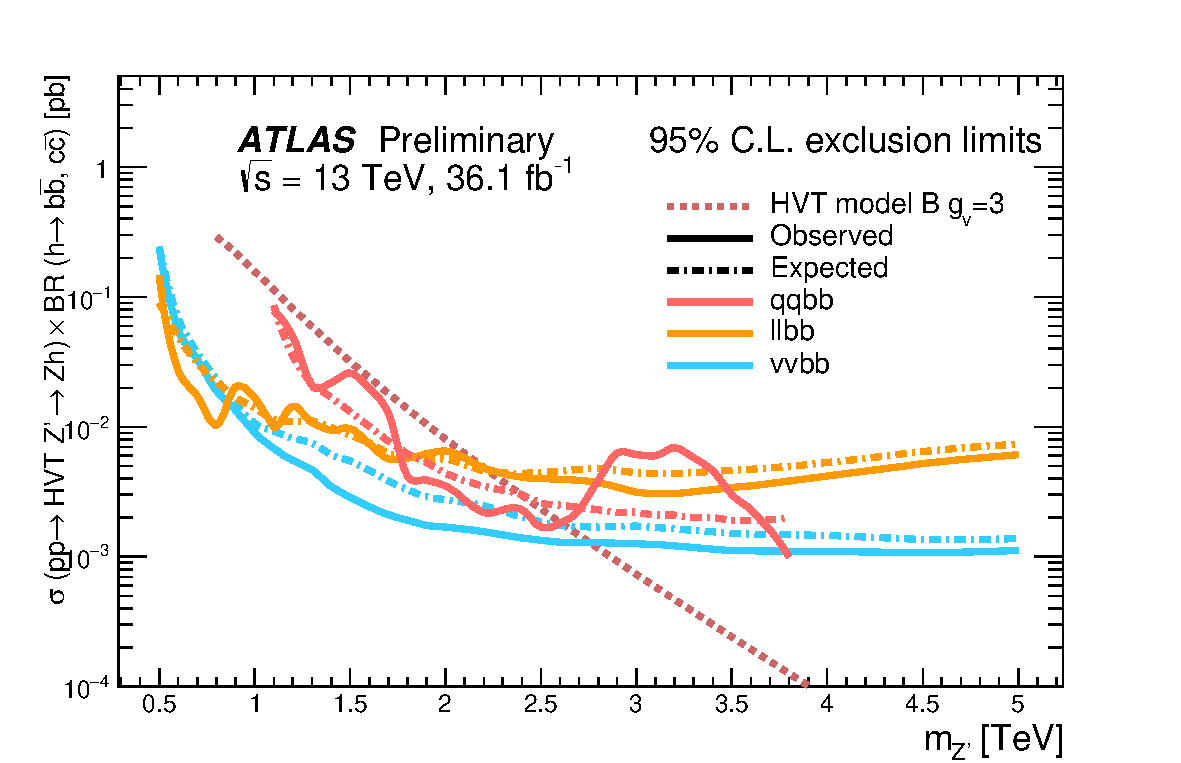
\includegraphics[width=.495\textwidth]{figures/ATLAS_Diboson_Summary_VV_ZP.pdf}
  \caption{The observed and expected limits on the product of the cross-section and branching fraction $\sigma \mathcal{B} (W' \rightarrow WH)$ for a spin-1 $W'$ (left) and $\sigma \mathcal{B} (Z' \rightarrow ZH)$ for a spin-1 $Z'$ (right), as a function of the reconstructed mass of the diboson resonance. The colored lines show the theoretical predictions for the HVT model B.}
  \label{fig:theory_ATLAS_Diboson_Summary_VH}
\end{figure}
%Data collected by ATLAS and CMS experiments are used to set limits on the HVT resonance masses and coupling parameters. Experimental results, both from Run 1 LHC data (at a center-of-mass energy of 8 TeV) brought to the following conclusions. A weakly coupled resonance, in the context of benchmark model A ($g_V = 1$) was excluded up to 3 TeV by Run 1 data. By looking at parton luminosities in fig.\ref{fig:HVT_DY_partolumi}, in data produced by LHC proton-proton collision at 14 TeV, collected for an integrated luminosity of 300 $\mbox{fb}^{-1}$, sensitivity was expected to increase up to $m_V \approx 6$ TeV. A strongly coupled resonance, in the context of benchmark model B ($g_V = 3$) is excluded up to 2 TeV by Run 1 data. Data produced by LHC at 14 TeV should have increased the sensitivity up to $m_V \approx 3-4$ TeV.\\
%No evidence of HVT resonances has been observed so far. ~\cite{CMS-PAS-B2G-16-007,Aad:2015ipg}. The most stringent limits have been set by LHC data collected in 2016 during Run 2 proton-proton collisions, performed at a center-of-mass energy of 13 TeV.

\clearpage
\section{Warped extra dimension}
\label{sec:theory_WED}
The Randall-Sundrum model~\cite{Randall:1999ee,Randall:1999vf} (RS1) proposes the introduction of one additional warped dimension in order to solve the hierarchy problem. The metric of the 5-dimensional space (a slice of $AdS_5$) generates an exponential hierarchy between the electroweak and Planck scales, associated respectively to the TeV three-brane, where the SM particles are confined, and the Planck three-brane. As a consequence of the new geometry, spin-2 massive gravitons are predicted to exist.\\
The bulk extension of the Randall-Sundrum model~\cite{Agashe:2007zd,Fitzpatrick:2007qr} states that the SM fields can propagate in the extra dimension. Light fermions are near the Planck brane, heavy fermions are close to the TeV brane, while the Higgs sector is confined in the TeV brane. Higgs couplings to the heavy fermions are therefore expected to be stronger: this naturally arising hierarchy of the masses of the SM fields gives a solution to the flavour problem. In this scenario, the fermionic decays of the bulk gravitons are suppressed, while the bosonic decays are preferred.

\subsection{Randall-Sundrum original model (RS1)}
\label{sec:RS1}
The existence of additional $n$-dimensions implies that the effective Planck scale observed in 4-dimensions, $M_{PL} = 1.2209 10^{19}$ GeV, is related to the fundamental 4+$n$-dimensional Planck scale, $M$, via the geometry. $M$ is expected to be of the order of the reduced $\overline{M}_{PL} = M_{PL}/2 \pi$. If the 4-dimensional and the $n$ additional metrics are factorizable, $\overline{M}_{PL}$ is the product of $M$ and the volume of the compact space $V_n$:
\begin{equation}
\overline{M}_{PL}^2 = V_n M^{2+n}.
\label{eq:theory_planck_mass}
\end{equation}
If $M \sim$ TeV, this implies that $V_n$ must be very large, hence the compactification scale $\mu~\sim~1/V_n^{1/n}$ is small (eV -- MeV for n=2 -- 7).  Given the smallness of $\mu$ when compared to the electroweak scale, the effects of the extra dimensions should be evident in SM processes. Since they are not observed, SM particles are assumed to be confined in a 4-dimensional space, the TeV three-brane, while only gravity is allowed to propagate into the 4+$n$-dimensional space, the bulk. This mechanism solves the hierarchy of the Higgs scale but introduces a new hierarchy between $\mu$ and $M$.\\
In the Randall-Sundrum model~\cite{Randall:1999ee,Randall:1999vf}, only one additional dimension is added. The geometry of the 5-dimensional bulk is non-factorizable, and it is a slice of $AdS_5$ spacetime.\footnote{An $n$-dimensional anti-de Sitter space ($AdS_n$) is a maximally simmetric Lorentiaz mainfold, that solves the Einstein equation with a negative curvature (negative cosmological constant).} The 4-dimensional metric is multiplied by an exponential function of the fifth dimension (the "warp" factor):
\begin{equation}
ds^2 = e^{-2 k r_c \phi} \eta_{\mu \nu} dx^{\mu} dx^{\nu} + r_c^2 d{\phi}^2;
\label{eq:theory_metric}
\end{equation}
$x^{\mu}$ are the usual 4-dimensional coordinates, $\eta_{\mu \nu} = diag(-1, 1, 1, 1)$ is the Minkowski metric, $k$ is a scale of order of $\overline{M}_{PL}$, $\phi$ is the coordinate of the extra dimension, $0 < |\phi| < \pi$, and $r_c$ is the compactification radius of this finite interval. 4-dimensional mass scales are obtained by multiplying the bulk masses by $e^{-2 k r_c \phi}$: given the exponential form of the warp factor, a small $r_c$ suffices for generating a large hierarchy between Planck and Higgs scales.\\
Two 4-dimensional three-branes are located at the boundaries of the fifth dimension: the visible brane at $\phi = \pi$; the hidden brane at $\phi = 0$, and their metrics are obtained starting from the bulk 5-dimensional metric $G_{MN}$, where $M,N = \mu, \phi$:
\begin{equation}
\begin{split}
 & g_{\mu \nu}^{\text{vis}} (x^{\mu}) = G_{\mu \nu} \left( x^{\mu}, \phi = \pi \right)\\
 & g_{\mu \nu}^{\text{hid}} (x^{\mu}) = G_{\mu \nu} \left( x^{\mu}, \phi = 0 \right).\\
\end{split}
\label{eq:theory_brane_metrics}
\end{equation}
The classical action is given by:
\begin{equation}
\begin{split}
 & S = S_{\text{gravity}} + S_{\text{vis}} + S_{\text{hid}}\\
 & S_{\text{gravity}} = \int d^4x \int_{-\pi}^{+\pi} d\phi \sqrt{-G} \left( -\Lambda + 2 M^3 \mathcal{R} \right)\\
 & S_{\text{vis}} = \int d^4x \sqrt{-g_{\text{vis}}} \left( \mathcal{L_{\text{vis}}} -V_{\text{vis}} \right)\\
 & S_{\text{hid}} = \int d^4x \sqrt{-g_{\text{hid}}} \left( \mathcal{L_{\text{hid}}} -V_{\text{hid}} \right),\\
\end{split}
\label{eq:theory_classical_action}
\end{equation}
where $G$ ($g$) is the trace of the $G_{MN}$ ($g_{\mu \nu}$) metric, $\Lambda$ is the cosmological constant in the bulk, $\mathcal{R}$ is the 5-dimensional Ricci scalar, $\mathcal{L}$ and $V$ are the lagrangian and the vacuum energy of the hidden and visible branes.\\
A 5-dimensional metric that preserves the 4-dimensional Poincar\'e invariance has the form:
\begin{equation}
ds^2 = e^{-2 \sigma(\phi)} \eta_{\mu \nu} dx^{\mu} dx^{\nu} + r_c^2 d{\phi}^2.
\label{eq:theory_poincare_metric}
\end{equation}
The Poincar\'e invariance guarantees that $r_c$ does not depend on $x^{\mu}$. Given~\ref{eq:theory_poincare_metric}, the solution of the 5-dimensional Einstein's equations simplifies into:
\begin{equation}
\sigma = r_c \left| \phi \right| \sqrt{\frac{- \Lambda}{24 M^3}}.
\label{eq:theory_einstein_solution}
\end{equation}
Furthermore, the Poincar\'e invariance imposes constraints to the vacuum energies and cosmological constant:
\begin{equation}
\begin{split}
 & V_{\text{hid}} = - V_{\text{vis}} = 24 M^3 k \\
 & \Lambda = -24 M^3 k^2.\\
\end{split}
\label{eq:theory_vacuum_energies}
\end{equation}
The final 5-dimensional metric is then:
\begin{equation}
ds^2 = e^{-2 k r_c \left| \phi \right|} \eta_{\mu \nu} dx^{\mu} dx^{\nu} + r_c^2 d{\phi}^2.
\label{eq:theory_metric_solution}
\end{equation}

\noindent A small $r_c$ is considered, so the effects of the fifth dimension on 4-dimensional spacetime can't be appreciated. A 4-dimensional effective field theory approach is therefore motivated, and its mass parameters are related to the bulk parameters, $M$, $k$ and $r_c$. In the Randall-Sundrum model, SM matter fields are confined in the TeV brane.\\
The massless gravitons, the mediators of the gravitational interaction in the effective field theory, are the zero modes ($h_{\mu \nu}$) of the quantum fluctuations of the classical solution (~\ref{eq:theory_metric_solution}):
\begin{equation}
ds^2 = e^{-2 k T(x) \left| \phi \right|} \left( \eta_{\mu \nu} + h_{\mu \nu}(x) \right) dx^{\mu} dx^{\nu} + T^2(x) d{\phi}^2,
\label{eq:theory_metric_perturbation}
\end{equation}
where the usual Minkowski metric has been replaced by $\overline{g}_{\mu \nu} (x) = \eta_{\mu \nu} + h_{\mu \nu}$; $h_{\mu \nu}$ are the tensor fluctuations around the Minkowski space, and represent both the physical graviton in 4-dimensions and the massless mode of the Kaluza-Klein decomposition of the bulk metric. $r_c$ is the vacuum expectation value of $T(x)$.\\
By substituting eq.~\ref{eq:theory_metric_perturbation} in the classical action~\ref{eq:theory_classical_action}, an effective action can be extracted, and in particular the curvature term holds:
\begin{equation}
S_{\text{eff}} \sim \int d^4 x \int_{-\pi}^{+\pi} d \phi 2 M^3 r_c e^{-2 k r_c \left| \phi \right|} \overline{\mathcal{R}} \sqrt{-\overline{g}},
\label{eq:theory_effective_action}
\end{equation}
where $\overline{g}$ is the trace of $\overline{g}_{\mu \nu}$ and $\overline{\mathcal{R}}$ is the 4-dimensional Ricci scalar of $\overline{g}_{\mu \nu}$ metric. In this effective 4-dimensional action, the $\phi$ dependence can be integrated out, and the 4-dimensional Planck mass can be calculated:
\begin{equation}
\overline{M}_{PL}^2 = M^3 r_c \int_{-\pi}^{+\pi} d \phi e^{-2 k r_c \left| \phi \right|} = \frac{M^3}{k} \left( 1 - e^{-2 k r_c \pi} \right).
\label{eq:theory_effective_planck_mass}
\end{equation}
It can be shown~\cite{Randall:1999ee} that a field with a fundamental mass parameter $m_0$ in the bulk manifests in the visible three-brane with a physical mass $m$:
\begin{equation}
m = e^{-2 k r_c \pi} m_0.
\label{eq:theory_effective_masses}
\end{equation}
Scales $m \sim$ TeV are generated from $m_0 \sim \overline{M}_{PL}$ if $e^{k r_c \pi} \sim 10^{15}$. This relation stands still when Higgs field is introduced and confined in the visible three-brane:
\begin{equation}
v = e^{-2 k r_c \pi} v_0,
\label{eq:theory_effective_Higgs_vev}
\end{equation}
where $v$ is the Higgs vacuum expectation value in the TeV brane and $v_0$ is the 5-dimensional Higgs v.e.v.\\
The hierarchy problem is then solved by the exponential warp factor. The weakness of gravity in the TeV three-brane is motivated by the small overlap of the graviton wave function.\\
In order to calculate the mass spectrum of the graviton in the TeV brane, the tensor fluctuations of the Minkowski metric are expanded into a Kaluza-Klein (KK) tower $h_{\mu \nu}^{(n)}$:
\begin{equation}
h_{\mu \nu}(x, \phi) = \sum_{n=0}^{\infty} h_{\mu \nu}^{(n)}(x) \frac{\chi^{(n)}(\phi)}{\sqrt{r_c}}.
\label{eq:theory_RS_KK_tower}
\end{equation}
Once a suitable gauge is chosen, \textit{i.e.} $\eta^{\mu \nu} \partial_{\mu} h_{\nu \alpha}^{(n)} = \eta^{\mu \nu} h_{\mu \nu}^{(n)} = 0$, the equation of motion of $h_{\mu \nu}^{(n)}$ becomes the Klein-Gordon relation, where $m_n^G \geq 0$:
\begin{equation}
\left( \eta^{\mu \nu} \partial_{\mu} \partial_{\nu} - (m_n^G)^2 \right) h_{\mu \nu}^{(n)}(x)= 0.
\label{eq:theory_RS_KK_KleinGordon}
\end{equation}
By substituting eq.~\ref{eq:theory_RS_KK_tower} into Einstein's equation, the solutions for $\chi^{(n)}(\phi)$ (commonly called "profiles") are~\cite{Davoudiasl:1999jd,Gherghetta:2000qt}:
\begin{equation}
\chi^{(n)}(\phi) = \frac{e^{2 \sigma}}{N} \left[ J_2(z_n^G) + \alpha_n Y_2(z_n^G) \right],
\label{eq:theory_RS_KK_tower_profile}
\end{equation}
where $J_2$ and $Y_2$ are second order Bessel functions, $N$ is the normalization of the wavefunction, $\alpha_n$ are coefficients and $z_n^G = m_n^G e^{\sigma(\phi)}/k$. $m_n^G$ is the mass of the $n$-mode, and it depends on the roots of the Bessel functions $z_n^G = \left( 3.83, 7.02, 10.17, 13.32, ... \right)$. In the limit $m_n^G/k \ll 1$ and $e^{k r_c \pi} \gg 1$:
\begin{equation}
m_n^G = k z_n^G(\pi) e^{-k r_c \pi}.
\label{eq:theory_RS_KK_tower_mass}
\end{equation}
The interactions between the graviton KK modes and the matter fields in the TeV brane can be derived from the 4-dimensional effective Lagrangian, once $h_{\mu \nu}$ is replaced by its KK decomposition:
\begin{equation}
\mathcal{L} = - \frac{1}{\overline{M}_{PL}} T^{\mu \nu}(x) h_{\mu \nu}^{(0)} - \frac{1}{e^{-k r_c \pi} \overline{M}_{PL}} T^{\mu \nu}(x) \sum_{n=1}^{\infty}h_{\mu \nu}^{(n)}(x);
\label{eq:theory_RS_KK_lagrangian}
\end{equation}
$T^{\mu \nu}$ is the space energy-momentum tensor of the matter fields. The zero mode of the gravitons coupling is $1/\overline{M}_{PL}$, while higher order KK modes couplings to all SM fields are suppressed by $e^{-k r_c \pi} \overline{M}_{PL}$, that is of the order of the TeV scale. Spin-2 KK masses and couplings are hence determined by the TeV scale, or, equivalently, KK gravitons are close to the TeV brane. This implies that KK gravitons can be produced via $q \bar{q}$ or gluon fusion, and that a leptonic decay of the resonance could represent a very clear signal signature.

\subsection{Bulk extension of RS1: graviton production and decays}
\label{sec:BG}
An extension of the original RS1 formulation has been proposed. It states that the usual SM fields are no longer confined in the TeV brane, but they are the zero modes of the corresponding 5-dimensional SM fields. If first and second generation fermions are close to the Planck brane, contribution to flavour changing neutral currents by higher-dimensional operators are suppressed. These contributions are excluded by electroweak precision tests, but they were not prevented in original RS1. The second motivation behind the choice is, as mentioned previously, the naturally arising flavour hierarchy: first and second generation quarks have small Yukawa couplings to the Higgs sector, confined in the TeV brane, while top quark and bosons have stronger Yukawa couplings.\\
In this picture, couplings between higher-order KK gravitons and light fermions are strongly suppressed, resulting into a negligible KK gravitons production via $q \bar{q}$, whilst gluon fusion production becomes dominant. KK gravitons decay into top quarks and Higgs bosons are dominant, given that both their profiles are near the TeV brane, while leptonic decays are negligible. Via the equivalence theorem, the Goldstone bosons are equivalent to the longitudinally polarized weak bosons, $W_L^{\pm}$ and $Z_L$, that have profiles close to the TeV brane. Decays of KK gravitons into weak dibosons (and production in VBF) are comparable to di-top and di-Higgs decays.\\

\noindent The KK decomposition and the KK mass spectrum of the graviton have already been presented in sec.~\ref{sec:RS1}. The KK decomposition of a massless 5-dimensional gauge field $A_M(x, \phi)$ is similarly performed~\cite{Davoudiasl:2000wi}:
\begin{equation}
A_{\mu}(x, \phi) = \sum_{n=0}^{\infty} A_{\mu}^{(n)}(x) \frac{\chi^{(n)_A}(\phi)}{\sqrt{r_c}}.
\label{eq:theory_gauge_KK_tower}
\end{equation}
The profiles for the gauge fields are:
\begin{equation}
\chi^{(n)}_A(\phi) = \frac{e^{\sigma}}{N_A} \left[ J_1(z_n^A) + \alpha_n^A Y_1(z_n^A) \right],
\label{eq:theory_gauge_KK_tower_profile}
\end{equation}
where $J_1$ and $Y_1$ are first order Bessel functions. Similarly to eq.~\ref{eq:theory_RS_KK_tower_mass}, the mass spectrum of the gauge field is:
\begin{equation}
m_n^A = k z_n^A(\pi) e^{-k r_c \pi};
\label{eq:theory_RS_KK_tower_mass}
\end{equation}
the first roots of the Bessel functions are $z_n^A = \left( 2.45, 5.57, 8.70, 11.84, ... \right)$.

\noindent The Lagrangian expressing the interaction between the $m$ and $n$ modes of the bulk field $F$ to the $q$ KK gravitons mode $G$ is~\cite{Davoudiasl:2000wi}:
\begin{equation}
\mathcal{L}_{G-F} = \sum_{m,n,q} C_{mnq}^{FFG} \frac{1}{\overline{M}_{PL}} \eta^{\mu \alpha} \eta^{\nu \beta} h_{\alpha \beta}^{(q)} (x) T_{\mu \nu}^{(m,n)}(x),
\label{eq:theory_lagrangian_bulk_KK}
\end{equation}
$C_{mnq}^{FFG}$ is the overlap integral of the profiles:
\begin{equation}
C_{mnq}^{FFG} = \int \frac{d \phi}{\sqrt{k}} e^{t \sigma} \frac{\chi_F^{(m)} \chi_F^{(n)} \chi_G^{(q)}}{\sqrt{r_c}};
\label{eq:theory_overlap_integral}
\end{equation}
$t$ depends on the type of field considered.\\
The coupling between gluons and the $q$ KK graviton mode is given by:
\begin{equation}
C_{00q}^{AAG} = e^{k \pi r_c} \frac{2 \left[ 1 - J_0 (x_n^G)\right]}{k \pi r_c (x_n^G)^2 \left| J_2 (x_n^G)\right|}.
\label{eq:theory_overlap_integral_ggG}
\end{equation}
Once eq.~\ref{eq:theory_overlap_integral_ggG} is put in eq.~\ref{eq:theory_lagrangian_bulk_KK}, the most significant partial decay widths into the $q$ KK graviton mode are:
\begin{equation}
\begin{split}
 & \Gamma \left(G \rightarrow t_R \bar{t}_R \right) \sim N_c \frac{ \left[ \tilde{k} x_q^G \right]^2 m_q^G}{320 \pi} \\
 & \Gamma \left(G \rightarrow h h \right) \sim \frac{\left[ \tilde{k} x_q^G \right]^2 m_q^G}{960 \pi} \\
 & \Gamma \left(G \rightarrow W^+_L W^-_L \right) \sim \frac{\left[ \tilde{k} x_q^G \right]^2 m_q^G}{480 \pi} \\
 & \Gamma \left(G \rightarrow Z_L Z_L \right) \sim \frac{\left[ \tilde{k} x_q^G \right]^2 m_q^G}{960 \pi}, \\
\end{split}
\label{eq:theory_bulk_KK_partial_decay_widths}
\end{equation}
where $\tilde{k} = k/\overline{M}_{PL}$; the total decay width is:
\begin{equation}
\Gamma_G = \frac{13 \left[ \tilde{k} x_q^G \right]^2 m_q^G}{960 \pi}.
\label{eq:theory_bulk_KK_total_decay_width}
\end{equation}

\noindent Calculations, so far, have been performed considering $M \sim \overline{M}_{PL}$ and $k < M$, hypoteses under which the solution for the bulk metric (eq.~\ref{eq:theory_metric_solution}) is valid. Hence, $\tilde{k} = k / \overline{M}_{PL} \leq 1$ is taken as a reference interval. This has also phenomenological consequences on the width of the resonance, as stated in eq.~\ref{eq:theory_bulk_KK_total_decay_width}. The total decay width of the lightest KK graviton mode, compared to its mass, is shown as a function of $\tilde{k}$ in fig.~\ref{fig:theory_grav_width_vs_ktilda}~\cite{Oliveira:2014kla}. At $\tilde{k} = 1$, in the bulk scenario, the KK graviton width is expected to be few \% of its mass, up to 4 TeV (dotted red curve). The narrow width approximation holds, hence the resonance properties can be probed at the peak, neglecting the effects in the tails of the mass distribution.

\begin{figure}[!htb]
  \centering
    \includegraphics[width=.495\textwidth]{figures/1404_0102_fig.pdf}
  \caption{Width of the KK gravitons, in units of the mass of the resonance, as a function of the curvature parameter $\tilde{k}$. The red curves represent the bulk extension of RS1 original model for different mass hypoteses (from 500 GeV up to 4 TeV).}
  \label{fig:theory_grav_width_vs_ktilda}
\end{figure}

\noindent The total cross-section of a bulk graviton, produced at LHC in proton-proton interactions via gluon fusion (displayed in fig.~\ref{fig:theory_KK_gg_prod}), decaying into a couple of vector bosons (for the purpose of this thesis, a final state with two longitudinally polarized $Z$ bosons is considered) is expressed as a function of the parton level cross-section $\hat{\sigma}$, the gluon parton distribution functions $f_q$, the momentum transfer $Q^2 \sim (m_q^G)^2$ and the center-of-mass energy $s$:
\begin{equation}
\sigma(pp \rightarrow ZZ) = \int dx_1 dx_2 f_g(x_1,Q^2) f_g(x_2, Q^2) \hat{\sigma}(x_1 x_2 s).
\label{eq:theory_cross_section_bulk}
\end{equation}
The differential parton level cross-section, averaged over colors and initial spin states, is (hatted quantities are calculated in the center-of-mass frame):
\begin{equation}
\frac{d \hat{\sigma}(gg \rightarrow ZZ)}{d \cos{\hat{\theta}}} \approx \frac{ \left| \mathcal{M}_{+-00}\right|^2}{1024 \pi \hat{s}},
\label{eq:theory_parton_level_cross_section_bulk}
\end{equation}
where $\left| \mathcal{M}_{+-00}\right|$ is the matrix element of the dominant contribution in $gg \rightarrow VV$ process ($\Gamma_G$ is defined in eq.~\ref{eq:theory_bulk_KK_total_decay_width}, $a$, $b$ are color factors):
\begin{equation}
\mathcal{M}_{+-00} (g^a g^b \rightarrow VV) = -C_{00q}^{AAG} e^{-k \pi r_c} \left( \frac{x^G_n \tilde{k}}{m_n^G}\right)^2 \sum_n \frac{\delta_{ab} \mathcal{A}_{+-00}}{\hat{s} - {m_n^G}^2 +i \Gamma_G m_n^G}.
\label{eq:theory_KK_matrix_elements}
\end{equation}
The relevant amplitudes taken account in the matrix element calculation are~\cite{Agashe:2007zd}:
\begin{equation}
%\begin{split}
\mathcal{A}_{+-00} = \mathcal{A}_{-+00} = \frac{\left( 1 - 1/\beta_Z^2 \right) \left( \beta_Z^2 -2\right) \left[ (\hat{t} - \hat{u})^2 - \beta_Z^2\hat{s}^2 \right] \hat{s} }{8 M_Z^2},
%\end{split}
\label{eq:theory_KK_amplitudes}
\end{equation}
where $\beta_Z^2 = 1- 4M_Z^2/\hat{s}$ and $M_Z$ is the mass of the $Z$ boson.

\begin{figure}[!htb]
  \centering
\feynmandiagram [horizontal=a to b] {
  i1 [particle=\(g\)] -- [gluon] a -- [gluon] i2 [particle=\(g' \)],
  a -- [red!80!black, boson, edge label=\(G\), very thick] b,
  f1 [particle=\(Z\)] -- [boson] b -- [boson] f2 [particle=\(Z\)],
};
\caption{Gluon fusion production mechanism for a KK graviton that decays in a couple of $Z$ bosons.}
\label{fig:theory_KK_gg_prod}
\end{figure}

%\newpage
\subsection{Search for KK bulk gravitons at LHC}
\label{sec:theory_KK_limits_LHC}
No evidence of spin-2 bulk graviton resonances has been observed so far at LHC experiments. Data collected by ATLAS and CMS detectors are used to set limits on the graviton masses, generally considering different curvature parameter $\tilde{k}$ hypoteses, once assured the narrow width approximation is still valid (up to $\tilde{k} \sim 1$). The most stringent limits have been set with Run 2 data.

\vspace*{1\baselineskip}

\noindent Many results of the diboson searches performed at CMS and already presented in sec.~\ref{sec:theory_HVT_limits_LHC} are interpreted in the context of the bulk gravitons, together with the additional final states $WZ, ZZ \rightarrow \ell \bar{\ell} \nu \bar{\nu}$~\cite{CMS-PAS-B2G-16-023} and $HH \rightarrow b\bar{b} b \bar{b}$~\cite{CMS-PAS-B2G-16-026}. The most interesting limit is provided by \cite{CMS-PAS-B2G-16-023}, that, under the hypotesis $\tilde{k} = 0.5$, excludes a spin-2 bulk graviton with a mass lower than 800 GeV (fig.~\ref{fig:theory_B2G-16-023}).

\begin{figure}[!htb]
  \centering
    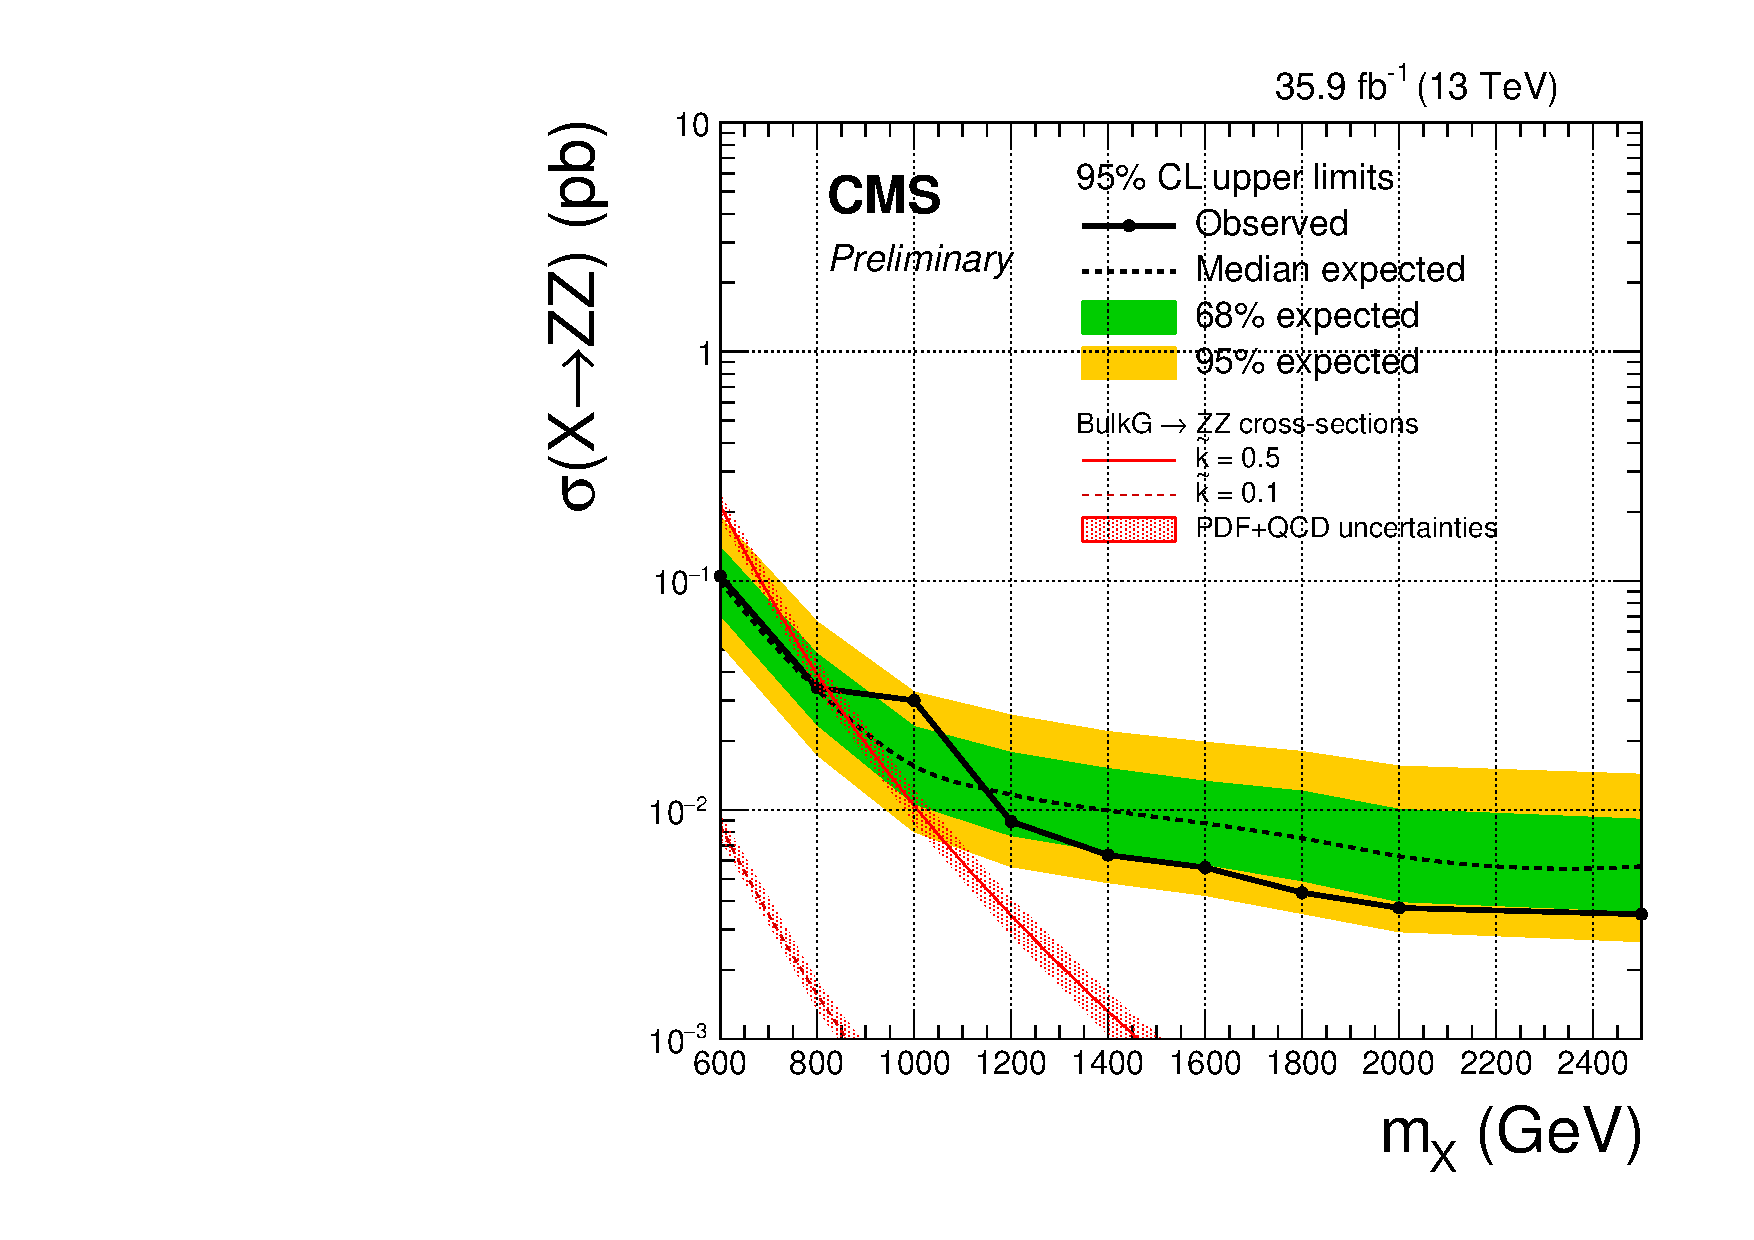
\includegraphics[width=.495\textwidth]{figures/B2G-16-023/Figure_005.pdf}
  \caption{The observed and expected limits, with 68\% and 95\% uncertainty bands, on the product of the cross-section and branching fraction $\sigma \mathcal{B} (G \rightarrow ZZ)$ for a spin-2 bulk graviton, as a function of the reconstructed mass of the diboson resonance. The colored lines show the theoretical predictions for $\tilde{k}=0.1$ and $0.5$.}
  \label{fig:theory_B2G-16-023}
\end{figure}

\vspace*{1\baselineskip}

%Revision
%
\noindent The results (or preliminary results) on bulk graviton searches in diboson final states, performed with 2016 data and published by the CMS Collaboration so far, are summarized in fig.~\ref{fig:theory_CMS_Diboson_Summary_graviton}. The dark orange curve and the pink curve correspond to two possible final states included the $(ZZ, WW) \rightarrow q\bar{q}q\bar{q}$ analysis~\cite{Sirunyan:2017acf,bib:CMS-PAS-B2G-17-001}; the light blue curve corresponds to the $ZZ \rightarrow \ell \ell \nu \nu$ analysis~\cite{CMS-PAS-B2G-16-023}; the green curve corresponds to the $HH \rightarrow b\bar{b} b \bar{b}$ analysis~\cite{CMS-PAS-B2G-16-026}; the light orange curve corresponds to the analysis discussed in this thesis~\cite{CMS-PAS-B2G-17-005}.

\begin{figure}[!htb]
  \centering
    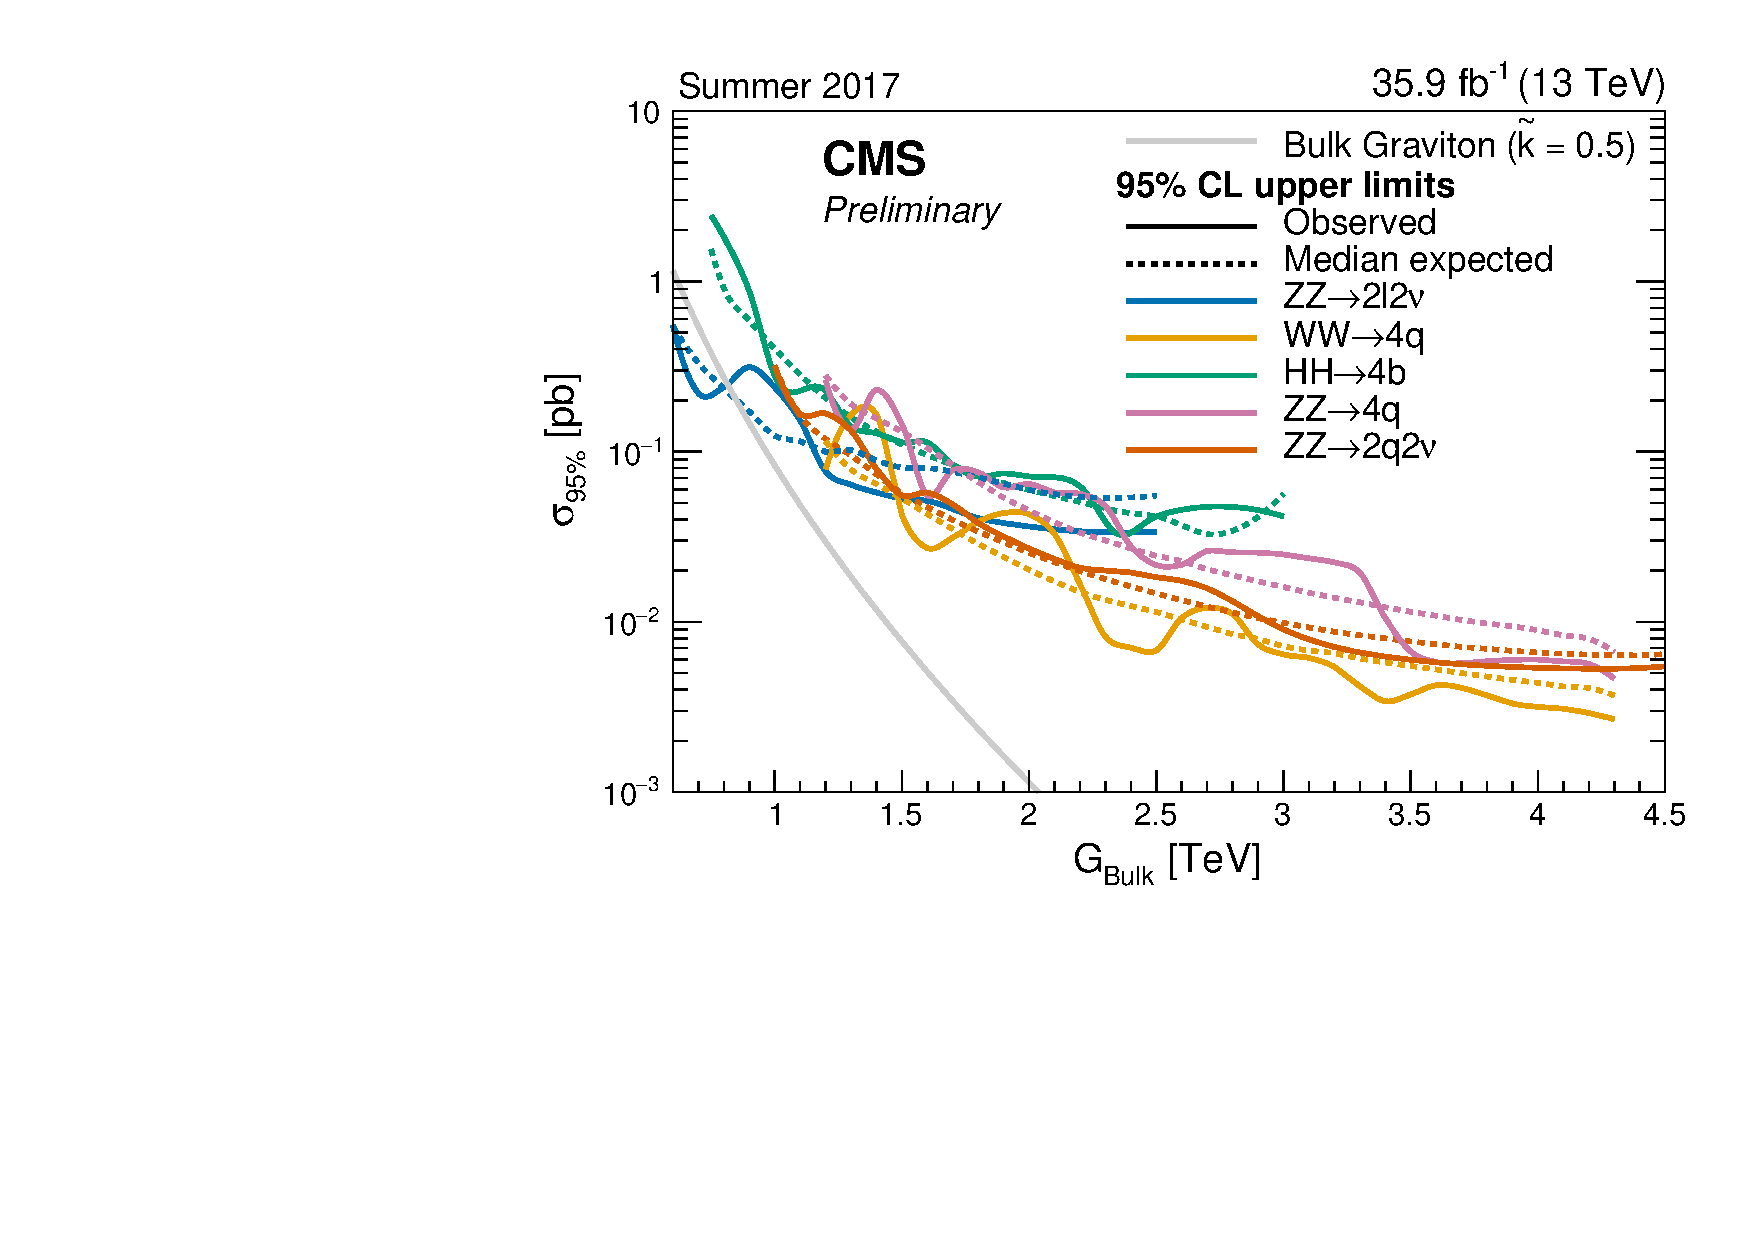
\includegraphics[width=.495\textwidth]{figures/combiLimitsBulkG_BulkG.pdf}
  \caption{The observed and expected limits on the product of the cross-section and branching fraction $\sigma \mathcal{B} (G \rightarrow (WW, ZZ))$ for a spin-2 bulk graviton, as a function of the reconstructed mass of the diboson resonance. The gray line show the theoretical prediction for the bulk graviton model, once assumed a curvature parameter $\tilde{k}=0.5$.}
  \label{fig:theory_CMS_Diboson_Summary_graviton}
\end{figure}

%\vspace*{1\baselineskip}
\clearpage

\noindent Similarly for ATLAS experiment, searches for diboson resonances in sec.~\ref{sec:theory_HVT_limits_LHC} have been interpreted in the graviton context. The most stringent limit is given by~\cite{ATLAS-CONF-2017-051}, where, under the assumption $\tilde{k}=1$, a spin-2 bulk graviton with mass lower than 1.76 TeV is excluded (fig.~\ref{fig:theory_ATLAS-CONF-2017-051}).

\begin{figure}[!htb]
  \centering
    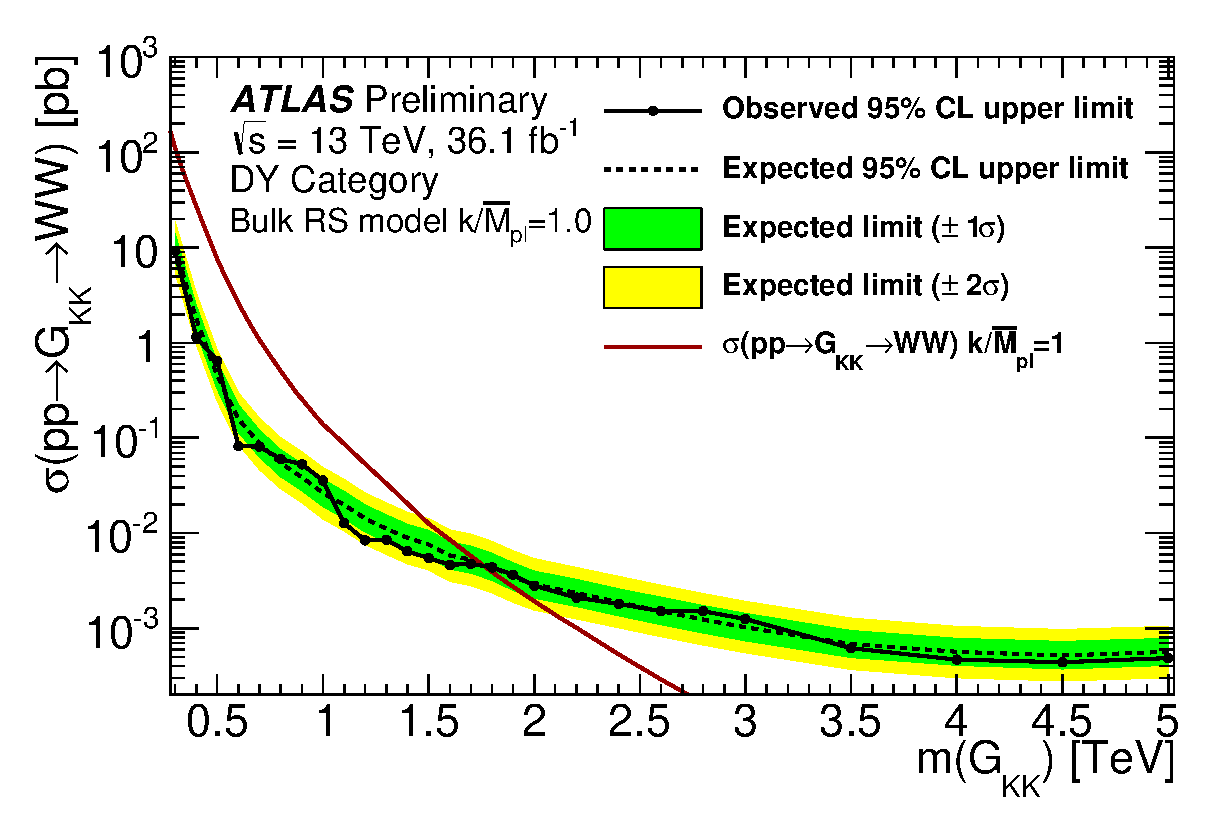
\includegraphics[width=.495\textwidth]{figures/ATLAS-CONF-2017-051_graviton.eps}
  \caption{The observed and expected limits, with 68\% and 95\% uncertainty bands, on the product of the cross-section and branching fraction $\sigma \mathcal{B} (G \rightarrow ZZ)$ for a spin-2 bulk graviton, as a function of the reconstructed mass of the diboson resonance. The colored lines show the theoretical predictions for $\tilde{k}=1$.}
  \label{fig:theory_ATLAS-CONF-2017-051}
\end{figure}

%CMS:\\
%VV all had 2017 B2G-17-001\\%~\cite{bib:CMS-PAS-B2G-17-001}\\
%VH all had 2017 B2G-17-002~\cite{bib:CMS-PAS-B2G-17-002}\\
%VZ 2l 2nu 2017 B2G-16-023~\cite{CMS-PAS-B2G-16-023}\\
%HH 4b 2017 B2G-16-026~\cite{CMS-PAS-B2G-16-026}\\
%VZ 2l 2q 2016 B2G-16-022~\cite{CMS-PAS-B2G-16-022}\\
%VH 2l 2b 2016 B2G-16-003~\cite{Khachatryan:2016cfx}\\
%VW 1l 1nu 2q 2016 B2G-16-020~\cite{CMS-PAS-B2G-16-020}\\
%VZ 2nu 2q B2G-17-005~\cite{CMS-PAS-B2G-17-005}\\
%$WZ, ZZ \rightarrow \ell \bar{\ell} \nu \bar{\nu}$~\cite{CMS-PAS-B2G-16-023}; $HH \rightarrow b\bar{b} b \bar{b}$~\cite{CMS-PAS-B2G-16-026}; SOLO GRAVITONI

%ATLAS:\\
%VV all had 2017 CERN-EP-2017-147~\cite{Aaboud:2017eta}\\
%VH all had 2017 CERN-EP-2017-111~\cite{Aaboud:2017ahz} \\ 
%VW 1l 1nu 2q full 2016 ATLAS-CONF-2017-051~\cite{ATLAS-CONF-2017-051}\\
%VW ICHEP 2016 CERN-EP-2017-146~\cite{ATLAS-CONF-2016-062}\\
%VH lnu 2b ATLAS-CONF-2017-055~\cite{ATLAS-CONF-2017-055}\\
%VZ ICHEP semileptonic  ATLAS-CONF-2016-082~\cite{ATLAS-CONF-2016-082}\\

%{\color{red} \bf discussion on k/MPL less 1 postponed}\\
%{\color{red} \bf zero-mode of graviton in the planck brane -- KK graviton in the TeV brane}\\
%{\color{red} \bf volume suppression vs yukawa suppression}\\

\clearpage



\chapter{The Large Hadron Collider and the CMS experiment}%Dummy
%%\begin{tcolorbox}[breakable,colback=black!5!white,colframe=red!80!black,width=\textwidth]
\chapter{The Large Hadron Collider and the CMS experiment}
%\end{tcolorbox}
\label{chap:LHC_CMS}
Brief intro to CERN and LHC
\begin{itemize}
\item research
\item technology
\item education
\item collaboration
\end{itemize}

\section{The Large Hadron Collider}
The Large Hadron Collider (LHC) is a 27 km ring structure designed for the acceleartion and collision of protons and heavy ions. It is situated approximatively 100 m underground, between France and Switzerland, in the Geneva area, and it is the most important of the CERN (Conseil europ\'een pour la recherche nucl\'eaire) facilities. In order to reduce the cost of the project, definetively approved in 1996, the LHC has been designed to fit the pre-existing underground tunnel of the Large Electron-Positron collider (LEP) [ref. 24 Jacopo], built to accelerate electrons and positrons and running until the year 2000.\\
Moving from an electron-positron collider to an hadron collider allowed to reach higher energies in the center-of-mass frame, since the syncrotron radiation loss is inversely proportional to the fourth power of the mass of the particle involved: hence, it is reduced by a factor $m_p/m_e \sim 10^3$. Furthermore, at a proton-proton collider it is possible to collect higher luminosities (and hence more statistics) with regards to, for example, a proton-antiproton collider, like Tevatron at Fermilab, in the USA.\\
In the LHC two identical beam pipes rings are designed to let protons circulate in opposite directions, in ultrahigh vacuum conditions ($10^{-11}$--$10^{-10}$ mbar) in order to avoid collisions with gas molecules. Given the reduced available diameter in the tunnel (4 m), the two proton beams are magnetically coupled. The collider is composed by 8 arc sections (48 km) driving protons around the ring, and straight sections (6 km) where beam control systems and detectors are inserted. Proton beams collide in four interaction points, where the four main LHC experiments are installed: ALICE, ATLAS, CMS, LHCb.

\begin{figure}[!htb]
  \centering
    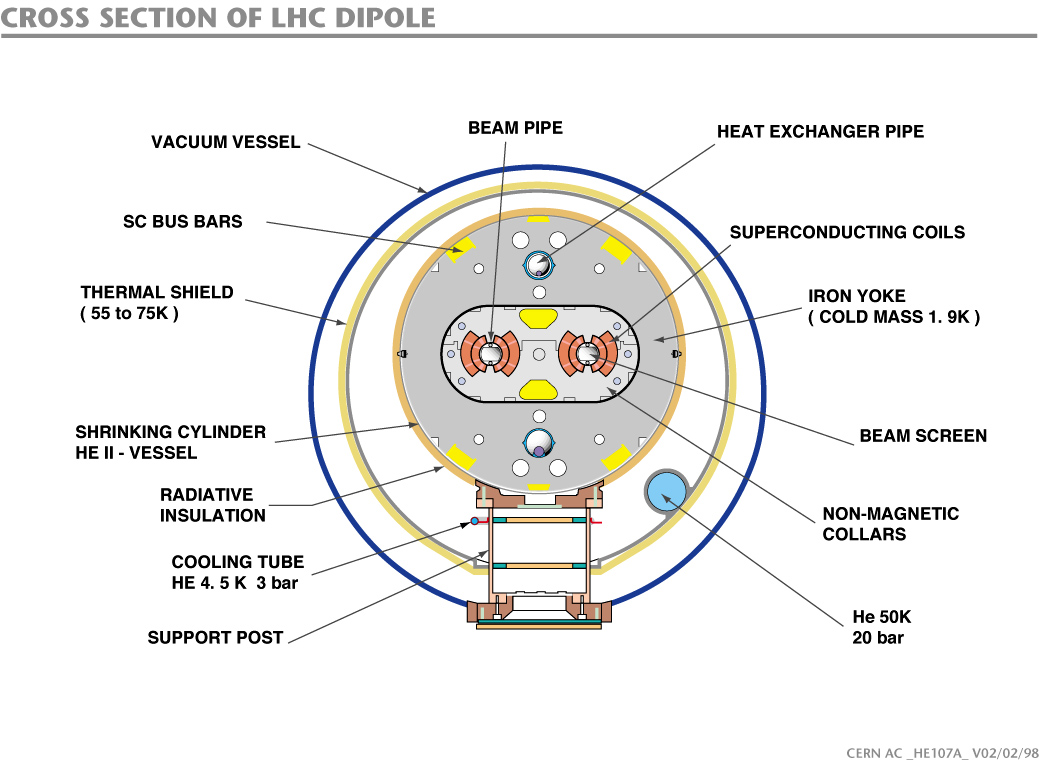
\includegraphics[width=.6\textwidth]{figures/LHC-magnets.jpg}
  \caption{Section of the LHC dipole magnet structure.}
  \label{fig:LHC_dipole}
\end{figure}

\noindent In fig.~\ref{fig:LHC_dipole}, a slice of the arc section is displayed. Around the beam pipes, two superconducting magnetic dipoles are located: they generate vertical magnetic fields in opposite directions. The superconducting coils are made of niobium-titanium, materials that are superconducting at very low temperature. At the LHC, they are kept at a temperature of 1.9 K (-$271.3^{\circ}$C) by a closed liquid helium circuit. A current of 11850 A flows through the magnets, without any energy loss due to electrical resistance, generating a magnetic field of 8.33 T. Magnets of higher order in multipole expansion (quadrupoles, sextupoles, octupoles, ...) are used to optimize the proton trajectories; in particular, quadrupoles allow to focus and squeeze the beams. Along the LHC ring here are 9593 magnets; 1232 are dipoles, 392 are quadrupoles.

\begin{figure}[!htb]
  \centering
    %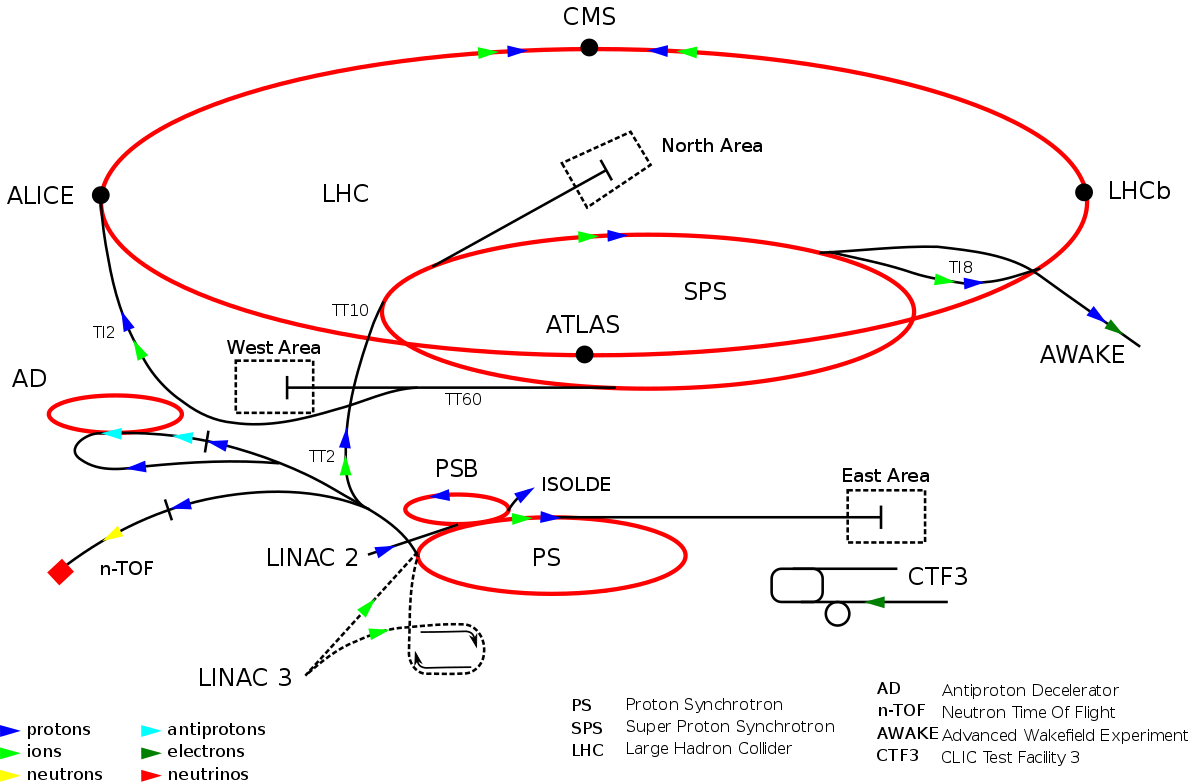
\includegraphics[width=.75\textwidth]{figures/Cern-accelerator-complex.png}\\
    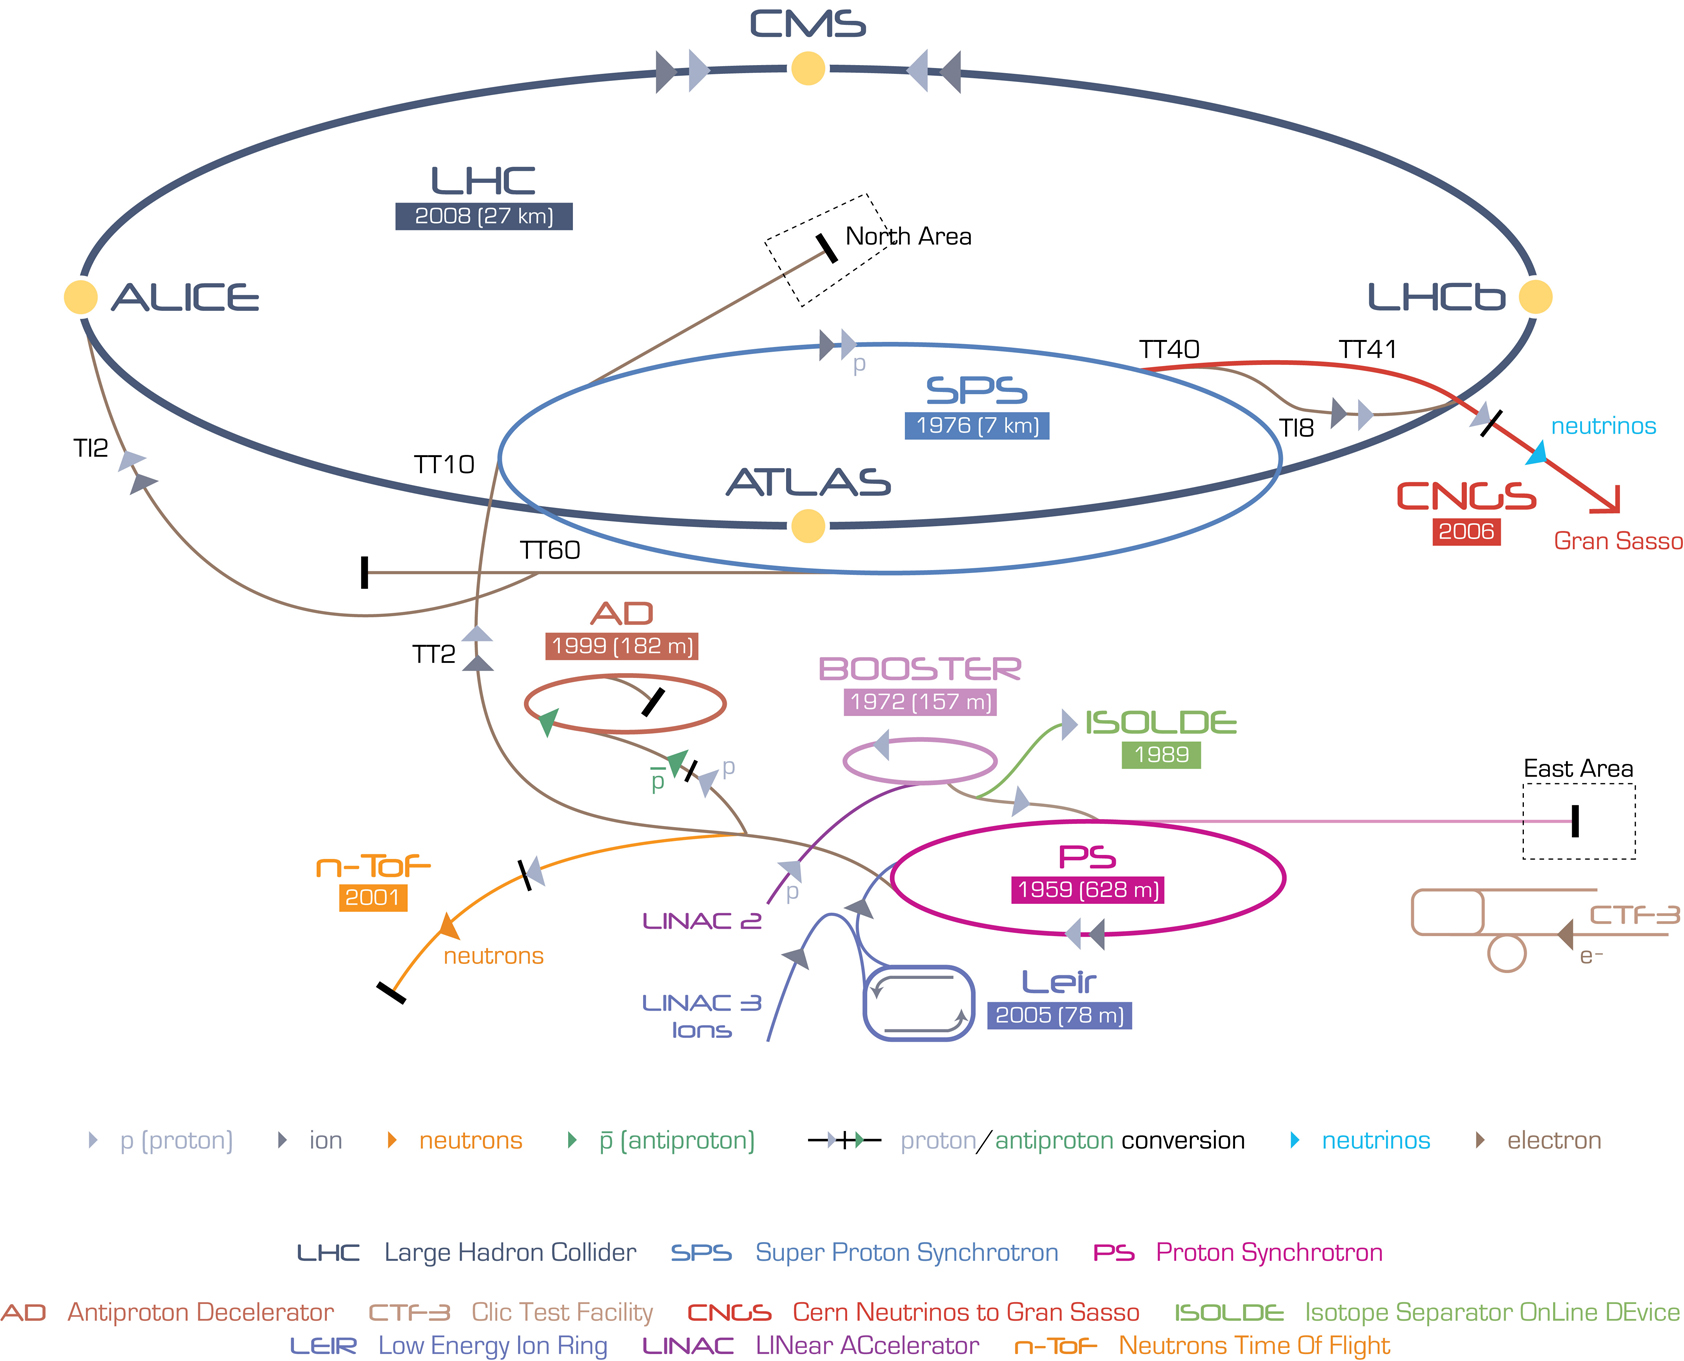
\includegraphics[width=.75\textwidth]{figures/Cern-Accelerator-Complex.jpg}
  \caption{The CERN accelerator complex.}
  \label{fig:LHC_accelerator_complex}
\end{figure}

\noindent The LHC represents the final step of the CERN accelerator complex, showed in fig.~\ref{fig:LHC_accelerator_complex}. Protons are extracted from hydrogen atoms and inserted in the linear accelerator Linac2, that brings them to an energy of 50 MeV. They circulate around a little synchrotron, Proton Synchrotron Booster, reaching an energy of 1.4 GeV, and then in the Proton Syncrhrotron (PS), where their energy is increased to 25 GeV. The second to last step is the Super Proton Synchrtotron, SPS, accelerating protons up to 450 GeV. They are finally injected in the Large Hadron Collider, where sixteen radiofrequency cavities (RF) accelerate protons inside each beam up to an energy of 6.5 TeV, providing a center-of-mass energy of 13 TeV when colliding. The RF cavities provide an accelerating electromagnetic field up to 5 MV/m (maximum voltage of 2 MV), that oscillates with a frequency of 400 MHz. Like the magnets, the cavities are kept at low temperature (4.5 K, or -$268.7^{\circ}$C) in order to allow superconducting conditions. The maximum beam energy can be reached in 15 minutes. After several hours of collisions ($\sim$ 10 hours), the quality of the beams deteriorates and they are extracted from the machine and dumped.\\

\noindent Protons circulate inside the LHC ring in bunches of $\sim10^{11}$ particles each, 80 mm long. Focusing magnets allow to reduce the bunch diameter down to 16 $\mu$m. Different bunches are separated by 25 ns (or, $\sim 7.5$ m), corresponding to a frequency of 40 MHz and an instantaneous (peak) luminosity (defined in eq.~\ref{eq:LHC_luminosity_def}) of $1.2 \times 10^{34}\mbox{ cm}^{-2} \mbox{s}^{-1}$. Given the structure of the beams, at every bunch crossing many protons interact simultaneously: this phenomenon is called pile-up. The designed maximum number of bunches is 2808.\\
%Protons with slightly different energies arriving earlier or later will be accelerated or decelerated so that they stay close to the energy of the ideal particle. In this way, the particle beam is sorted into discrete packets called "bunches". Top energy is reached in around 15 minutes, the bunches having passed the cavities around 1 million times.
%Queste frequenze elevate generano un problema noto con il nome di ``pile-up'', che consiste nel moltiplicarsi del numero di vertici primari di interazione. Ad un medesimo evento registrato prodotto dalle collisioni ogni 50 ns, infatti, corrispondono fino a 30 vertici di interazione; essi aumenteranno a 40 quando si arriver\`a a realizzare una collisione ogni 25 ns.\\

\begin{figure}[!htb]
  \centering
    \includegraphics[width=.5\textwidth]{PPD_results/int_lumi_per_day_cumulative_pp_2016.pdf}%
    \includegraphics[width=.5\textwidth]{PPD_results/int_lumi_per_day_cumulative_pp_2016_Golden_23Sep-PromEraH_Morion.png}

    \includegraphics[width=.5\textwidth]{PPD_results/int_lumi_per_day_pp_2016.pdf}%
    \includegraphics[width=.5\textwidth]{PPD_results/pileup_pp_2016.pdf}

  \caption{Luminosity in 2016 LHC data. Top-left plot: the cumulative integrated luminosity delivered by LHC (in blue) and recorded by CMS (in orange), as a function of the data taken period. Top-right plot: data recorded by CMS and declared as optimal for the physics analyses (in light orange), corresponding to a total integrated luminosity of 35.9 $\text{fb}^{-1}$. Bottom-left plot: maximum integrated luminosity per day. Bottom-right plot: number of proton interactions per bunch crossing (pile-up).}
  \label{fig:LHC_lumi}
\end{figure}

\noindent The main parameters that describes an hadronic collider are the center-of-mass energy, corresponding to the sum of the energies of the beams, and the instantaneous luminosity, that describes the frequency of the interactions among the bunches in the beams. If the bunches in the first beam contain $n_1$ protons, and the bunches in the second beam contain $n_2$ protons, and if the colliding area is $\Sigma$, the frequency of complete turns
around the ring is $f$, the instantaneous luminosity $\mathcal{L_{\text{inst}}}$ is:

\begin{equation}
\mathcal{L_{\text{inst}}} = f \frac{n_1 n_2}{\Sigma}.
\label{eq:LHC_luminosity_def}
\end{equation}

\noindent If a generic physics procces $i$ has a cross-section of $\sigma_i$, the interaction rate $R_i$ is:
\begin{equation}
R_i = \frac{dN_i}{dt}= \sigma_i \mathcal{L_{\text{inst}}},
\label{eq:LHC_interaction_rate}
\end{equation}
and the number of events recorded in the time interval $(0,\tau)$ is obtained by the integrated luminosity $\mathcal{L} = \int_0^{\tau} \mathcal{L_{\text{inst}}} dt$:
\begin{equation}
N_i = \sigma_i \int_0^{\tau} \mathcal{L_{\text{inst}}} dt.
\end{equation}

\noindent In fig.~\ref{fig:LHC_lumi}, a summary of the luminosity measurement in 2016 data is presented. The luminosity delivered by LHC is represented in blue, the recorded by CMS is in orange. The mean number of interaction per bunch crossing (pile-up) is presented as well. The average number of interactions per collision is 27, the maximum is around 50.

\subsection{Proton-proton interactions}
\begin{figure}[!htb]
  \centering
    \includegraphics[width=.5\textwidth]{figures/78events_PU.png}
  \caption{78 events.}
  \label{fig:pp_pileup}
\end{figure}
%Figura da CMS Collaboration, DAQ generic figures gallery online at http://cmsdoc.cern.ch/cms/TDR/DAQ/TDRweb/daqgenericjpg.htm
Proton-proton collisions allow to reach higher energies and luminosities, but the drawback is the complexity of the events when compared to electron-positron collisions: not only because of the increasing backgrounds due to strong interactions among partons, but also because the momenta of the proton partons taking part in the interaction are unknown; not to mention the problem of disentangling the tracks of the particles coming from the interesting hard interactions from the spectator pile-up interactions (in fig.~\ref{fig:pp_pileup}, 78 proton collisions were happening at the same bunch crossing).\\
The majority of the LHC events is represented by soft interactions, with low transverse momentum transfer, namely elastic and diffractive scatterings. In the so-called hard interactions, on the other hand, the transferred momentum among particles is high, allowing to produce massive resonant phenomena. These events manifest in peculiar final state signatures that can be distinguished from the soft interaction background.\\
At high momentum transfer (perturbative regime), a proton can be described as a collection of partons, each bringing a fraction $x$ of the initial beam momentum, whose distribution is described by the parton distribution functions (PDF), $f(x,Q^2)$, as a function of the Bjorken's variable and of the momentum transfer $Q^2$. At very high center-of-mass energies (13 TeV), the proton masses can be neglected; the available energy in the parton 1 and parton 2 scattering is unknown, $\sqrt{x_1 x_2 s}$. The total cross-section is given by:
\begin{equation}
\sigma = \int dx_1 f_1(x_1,Q^2) \int dx_2 f_2(x_2,Q^2) \sigma_{12}(x_1 p_1, x_2 p_2, Q^2),
\end{equation}
where $\sigma_{12}$ is the cross-section at parton level, and $f_1,f_2$ are the parton PDFs. In fig.~\ref{fig:LHC_pp_cross_section}, parton cross-sections are displayed as a function of the center-of-mass energy.

\begin{figure}[!htb]
  \centering
    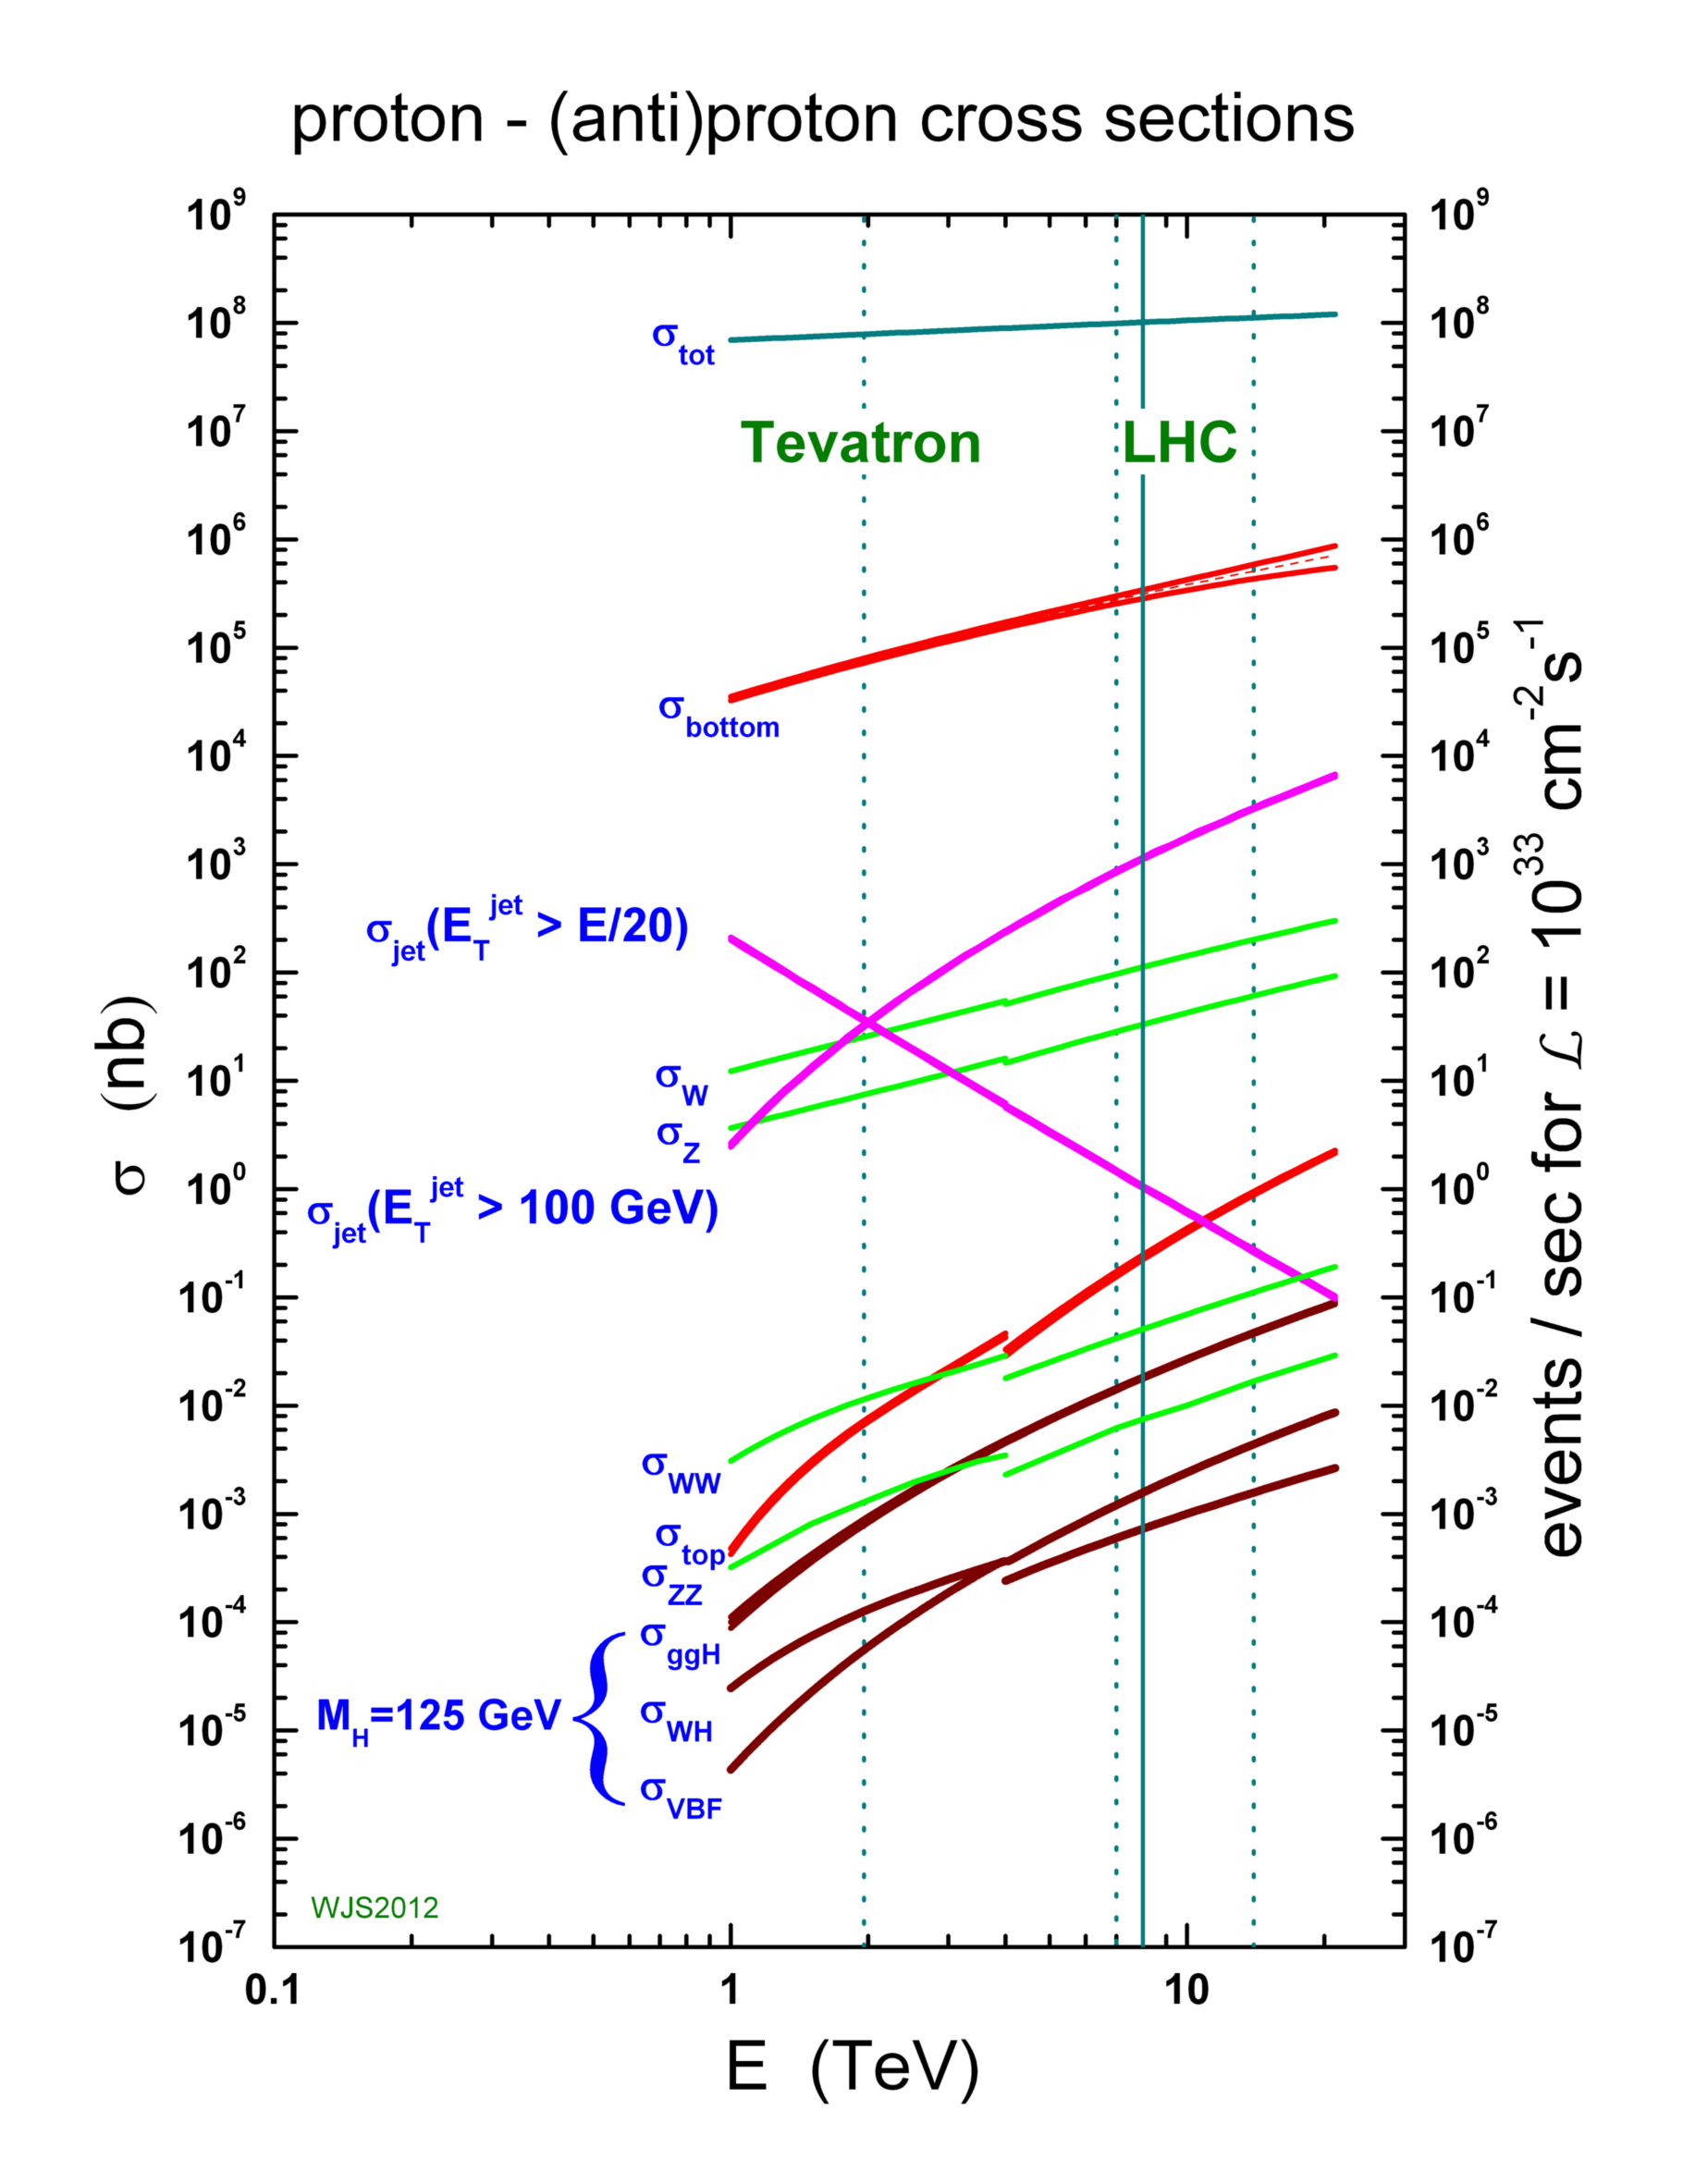
\includegraphics[width=.5\textwidth]{figures/crosssections2013.jpg}
  \caption{Cross-sections and number of expected events in proton-proton collisions, as a function of the center-of-mass energy. Rare phenomena, such as the Higgs boson production, can be observed at the LHC.}
  \label{fig:LHC_pp_cross_section}
\end{figure}

\section{CMS detector}

The Compact Muon Solenoid (CMS) is a multi-purpose detector built in the LHC ring. It is situated in a cavern 100 m underground, near Cessy, in France. It is a cylinder 22 m long, with a diameter of 15 m, and a weight of 12500 tons. Its physics programme includes the search for the Higgs boson (discovered in 2012), precision measurements of the Standard Model parameters and rare decays (physics of beauty quark), and search for new physics beyond the standard model (SUSY, exotic phenomena, dark matter, extra dimensions).\\
The CMS detector is structured in many layers of sub-detectors, giving different responses depending on the nature and the momentum of the particle passing through. The inner detectors have been finely segmented in order to afford the high radiation levels and particle multiplicity at the interaction point, so that the reduced occupancy of each layer allows to measure and distinguish precisely the primary vertices of the hard interactions from the pile-up events. A very precise time resolution is vital in order to synchronize all the subsystems together.\\
%La maggior parte dei processi fisici che si vogliono esplorare hanno basse sezioni d'urto, mentre, come \`e ben noto, i prodotti delle collisioni tra protoni sono dominati da elevati fondi QCD: CMS \`e progettato in modo da avere un'elevata capacit\`a di discriminazione degli eventi rari, sfruttando in particolare i canali comprendenti elettroni e muoni, e una grande precisione di misura dei vertici secondari, necessaria per distinguere i $\tau$ e gli adroni contenenti quark pesanti. L'elevata luminosit\`a nominale di LHC, come accennato, comporta il problema del pile-up: questi effetti possono essere ridotti utilizzando rivelatori ad elevata granularit\`a. L'occupazione si abbassa segmentando l'apparato in molti sottogruppi di rivelatori, al costo di dover ottenere un'ottima sincronizzazione tra di essi. L'alta frequenza di interazione, inoltre, necessita un'alta risoluzione temporale. Infine, gli elevati livelli di radiazione attorno al vertice richiedono apparati robusti e resistenti.

\begin{figure}[!htb]
  \centering
    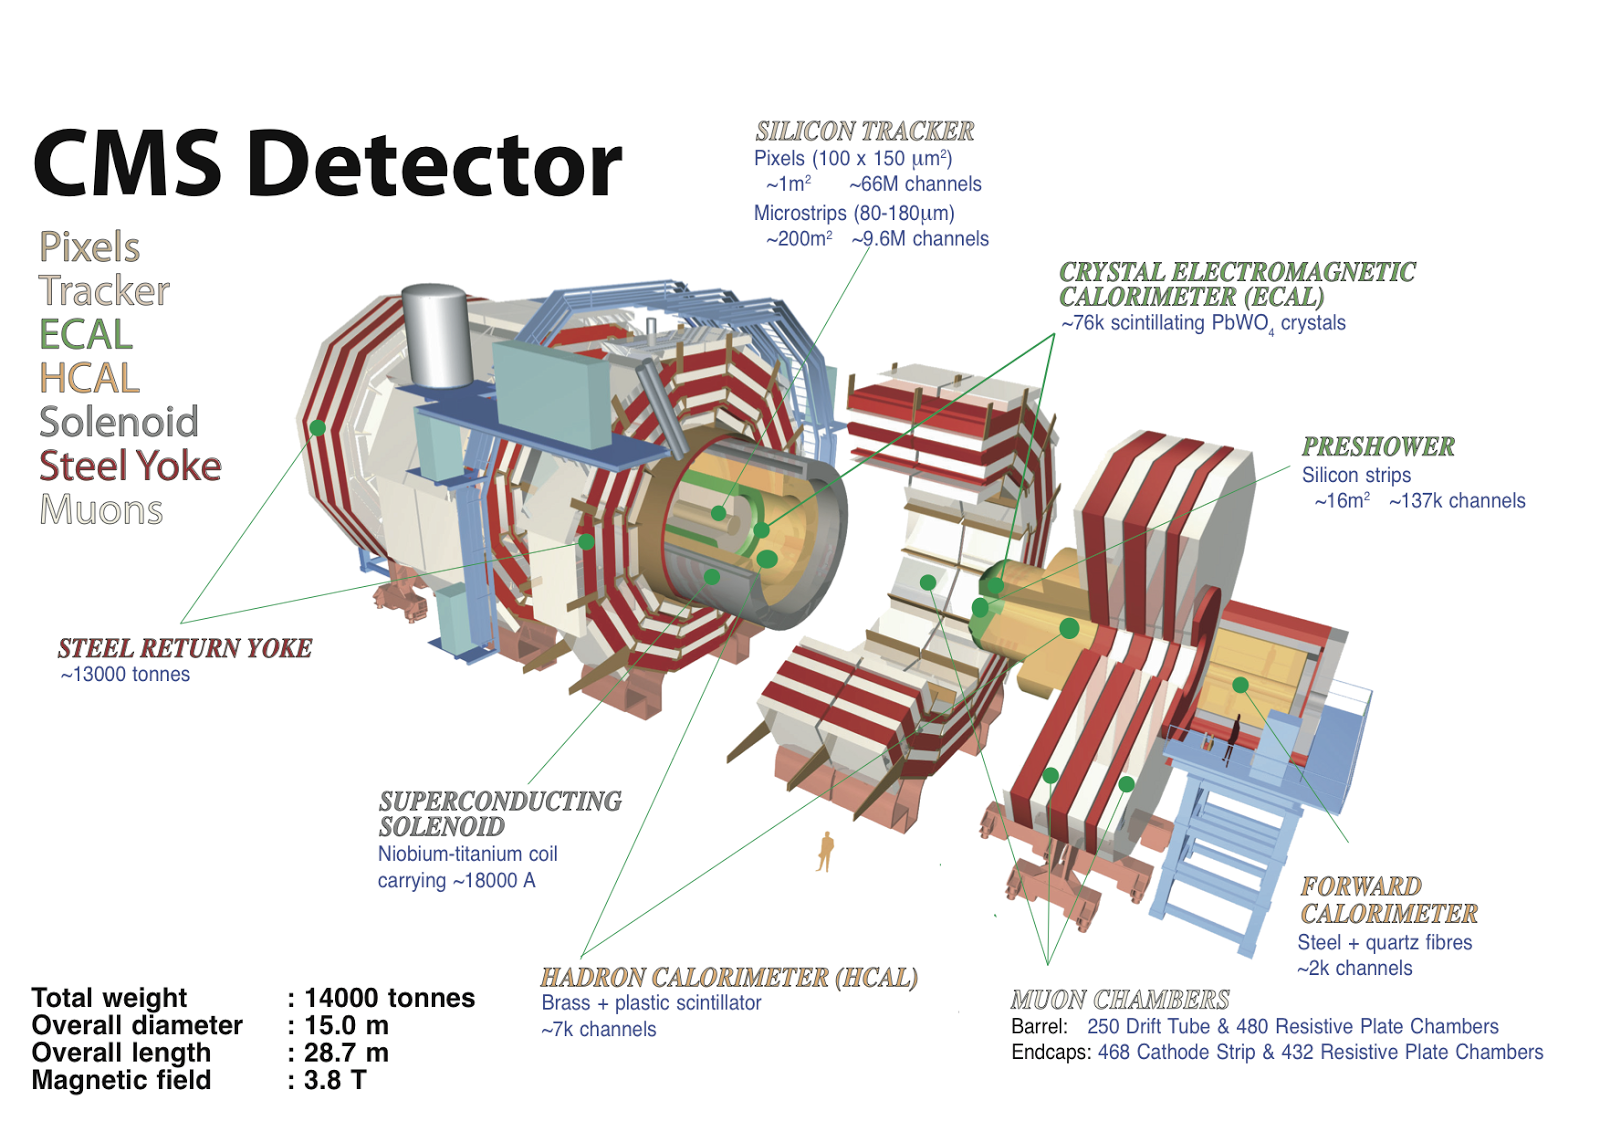
\includegraphics[width=.99\textwidth]{figures/cms_3d.png}
  \caption{The CMS experiment.}
  \label{fig:CMS_1}
\end{figure}

\noindent Fig.~\ref{fig:CMS_1} shows a sketch of the CMS detector. It is longitudinally segmented in the barrel region and two endcaps. In the forward region (over the endcaps), where the beam radiation is very intense, additional calorimeters have been placed. In fig.~\ref{fig:CMS_particles}, the mean path of a specific particle through the sub-detectors is represented, depending on its flavour.

\begin{figure}[!htb]
  \centering
    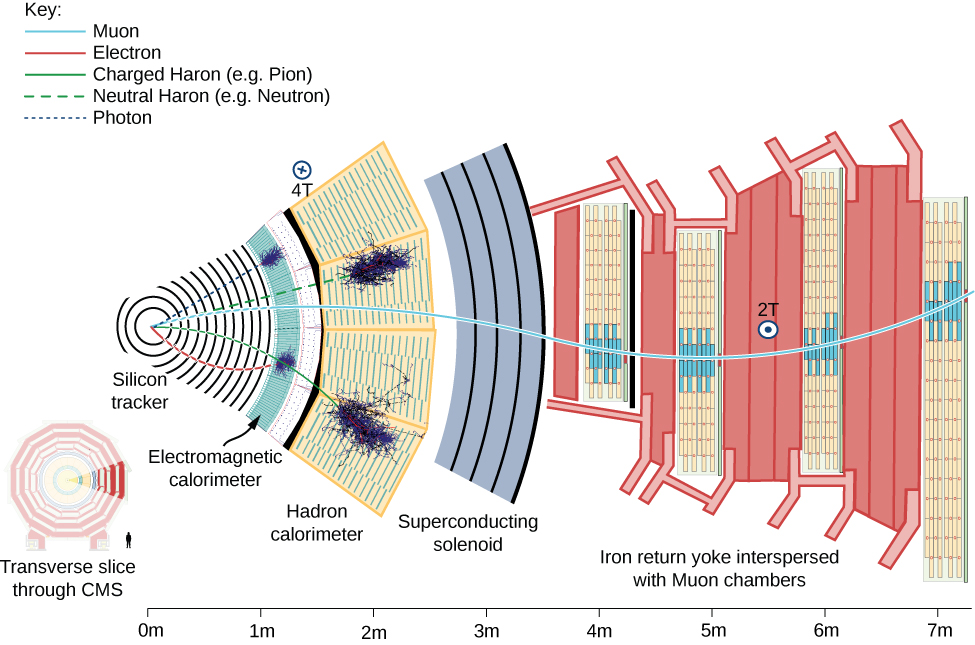
\includegraphics[width=.99\textwidth]{figures/CMS_particles.jpg}
  \caption{Mean path of a particle through the CMS detector. A muon, in light blue, passes through with a bended trajectory, depending on its momentum and charge, triggering signals in all the sub-systems. An electron, in red, leaves a track in the silicon tracker and is absorbed by the electromagnetic calorimeter. A neutral or charged hadron, in green, stops inside the hadronic calorimeter. A photon, dotted blue line, showers in the electromagnetic calorimeter, without leaving any track in the silicon detector.}
  \label{fig:CMS_particles}
\end{figure}

\subsection{The coordinate system}
The CMS cooridnate system is depicted in fig.~\ref{fig:CMS_CoordSys}. $x$ and $y$ are the coordinates in the transverse plane, $z$ is the longitudinal coordinate. The $x$ axis points at the center of the LHC ring, the $y$ axis points upward, the $z$ axis is along the beam direction. The azimuthal angle $\phi$ lays in the in the transverse plane, and it is measured starting from the $x$ axis; the radial coordinate is $r$. The polar angle $\theta$ lays in the plane $rz$. The transverse component of the 3-momentum, $\vec{p}_T$, is orthogonal to the beam axis and lays in the plane $xy$. The transverse energy is defined as the magnitude of $\vec{p}_T$: $E_T = E \sin{\theta}$.\\
Two other commonly used variables are the rapidity, $y$, and pseudorapidity, $\eta$, defined as functions of the particle energy $E$, the longitudinal component of the momentum $p_z$ and the 3-momentum modulus:
\begin{equation}
\begin{split}
 & y = \frac{1}{2} \log{\frac{E + p_z}{E - p_z}}\\
 & \eta = \frac{1}{2} \log{\frac{|\vec{p}| + p_z}{|\vec{p}| - p_z}} = -\log{\tan{\frac{\theta}{2}}}.
\end{split}
\end{equation}
When the considered particle is produced in the forward region, hence at $\theta = 0$, $\eta \rightarrow \infty$. When the particle is produced in the transverse plane, hence $\theta = \pi /2$, $\eta = 0$. At high energies, when the masses can be neglected, rapidity and pseudorapidity coincide; these variables are largely used at colliders because they are invariant under Lorentz boosts along the beam direction.

\begin{figure}[!htb]
  \centering
    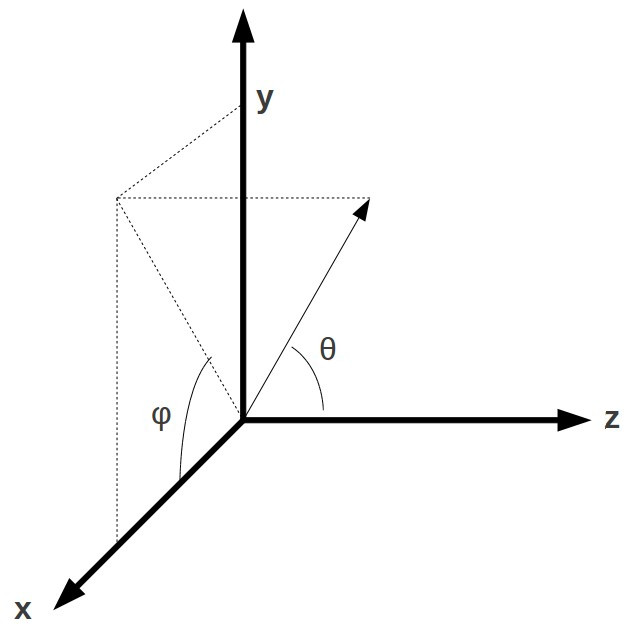
\includegraphics[width=.3\textwidth]{figures/CMS_CoordSys.jpg}
  \caption{CMS coordinate system.}
  \label{fig:CMS_CoordSys}
\end{figure}

\subsection{The magnet}
The CMS superconducting magnet is an hollow cylinder (13 m long, 6 m of diameter, showed in fig.~\ref{fig:CMS_solenoid}). In the niobium and titanium fibers that constitute the solenoid, an electrical current of 19 kA flows, providing a maximum magnetic field of 3.8 T and storing a maximum energy of 2.6 GJ. Superconductiong conditions are allowed by a liquid helium cooling system, keeping the solenoid at 4.5 K. In order to avoid stray fields, the magnetic field lines are closed by the return yoke, composed by 10 ktons of magnetized iron blocks, located in the outer part of CMS and alternated to the muon chambers. The homogeneus magnetic field inside the detector bends the trajectories of the charged particles, allowing the measurement of their momenta $p$, given the relation with the magnetic field strenght $B$ and the radial coordinate $R$ of the trajectory:
\begin{equation}
p [\text{GeV}] = 0.3 \times B [\text{T}] \times R [\text{m}]. 
\end{equation}

\begin{figure}[!htb]
  \centering
    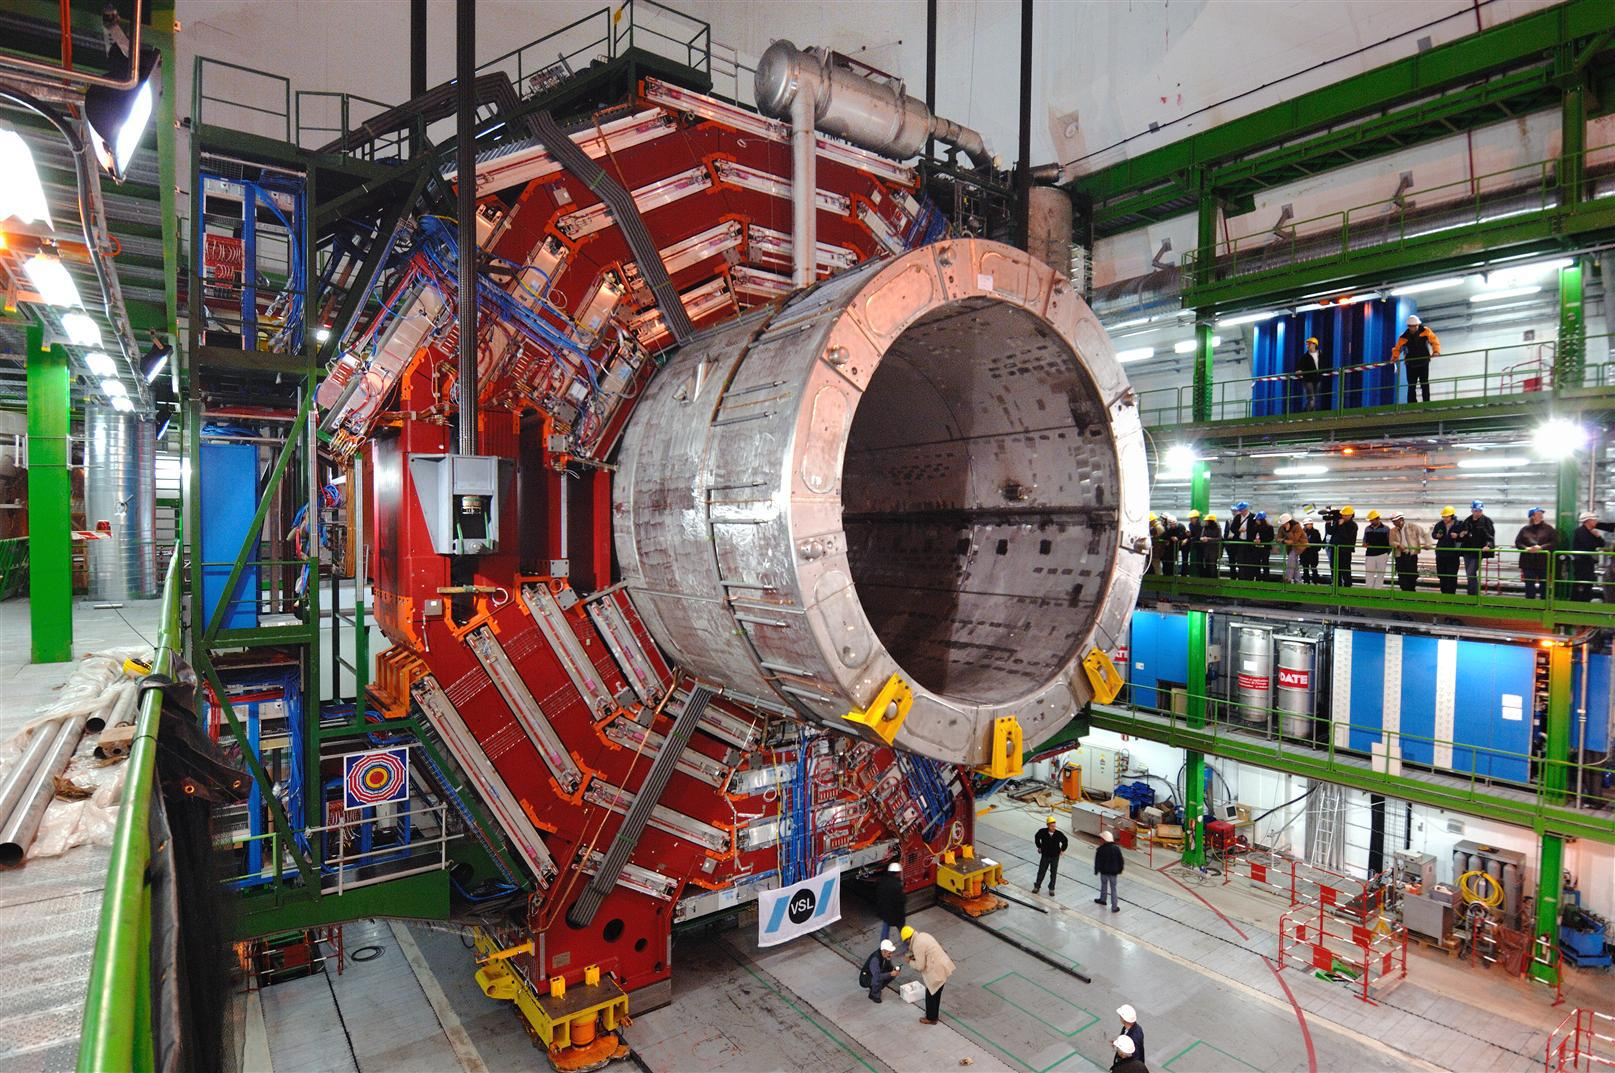
\includegraphics[width=.5\textwidth]{figures/CMS_solenoid.jpeg}
  \caption{Installation of the superconducting solenoid in the CMS cavern.}
  \label{fig:CMS_solenoid}
\end{figure}

\subsection{The tracking system}
\begin{figure}[!htb]
  \centering
    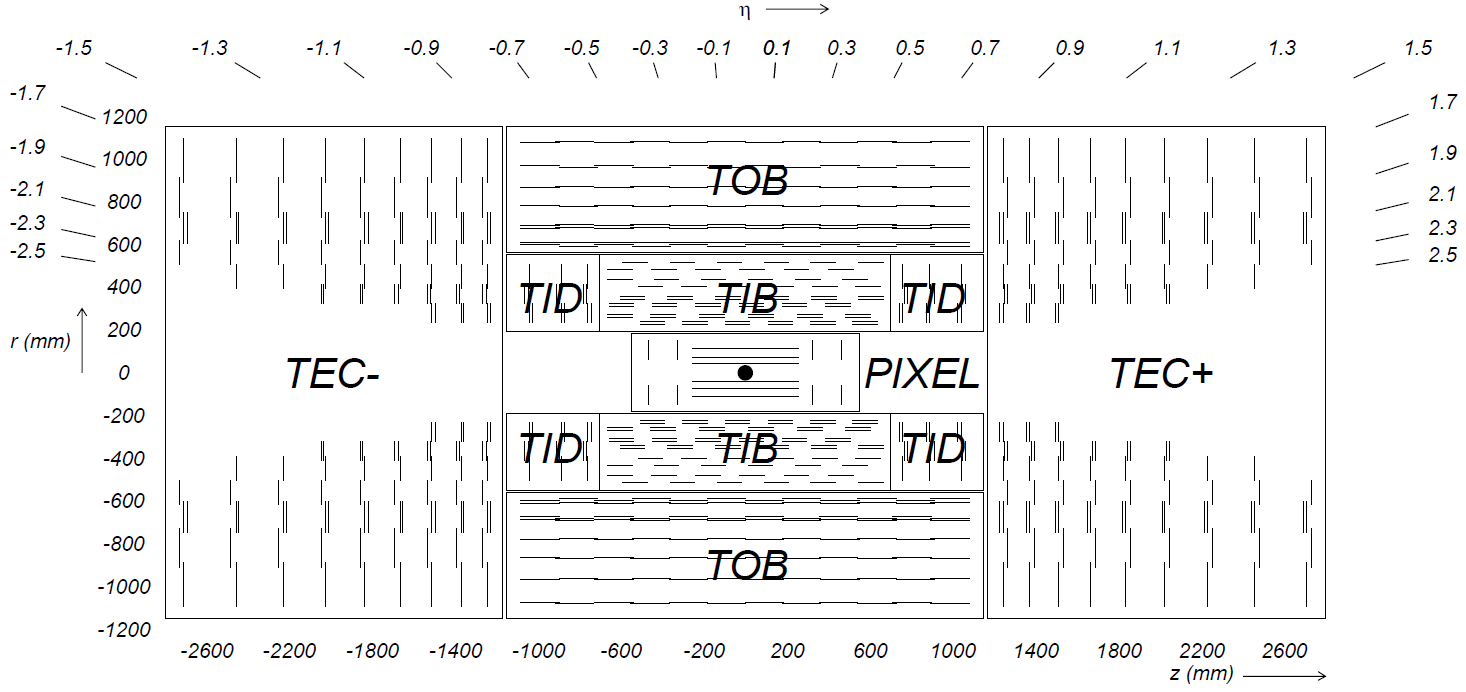
\includegraphics[width=.9\textwidth]{figures/cmstracker.png}
  \caption{The CMS tracking system: the inner pixel detector, close to the interaction point, and the outer strip detector.}
  \label{fig:CMS_tracker}
\end{figure}

The CMS tracking system is composed by a cylinder of silicon detectors (2.5 m of diameter and 5.8 m length). Their design allows a precise reconstruction of the tracks left by charged particles and of the interaction vertices, a fundamental tool to identify heavy quarks (charm, beauty) and leptons (taus).
Tracker detectors cover a pseudorapidity region of $|\eta|<2.5$ and have an active area of $210\text{ m}^2$. The two sub-detectors of the tracking system are the pixel detector, closer to the interaction point, and the strip detector, covering a radius of 0.2 -- 1.2 m. The high granularity of the pixels and micro strips allows to keep the occupancy at acceptable levels, given the high multiplicity of the tracks ($\sim$1 MHz/$\text{mm}^2$). The silicon detectors and the electronic cables are cooled down to a temperature of $\sim 10^{\circ}$ C. The structure of the tracking system is showed in fig.~\ref{fig:CMS_tracker}.

\subsubsection{The pixel detector}
The pixel detector is composed by 66 millions of silicon cells, whose dimensions are $100 \times 150 \text{ }{\mu{m}}^2$, 285 $\mu$m of thickness, placed in 1440 modules. Silicon cells are set in three layers in the barrel region and in two disks at each endcap. Barrel modules are disposed parallel to the magnetic filed, whilst at the endcap they are tilted by about $20^{\circ}$. 
%Il pixel detector \`e costituito da tre strati di rivelatori nel barrel e da due dischi agli endcaps. I moduli nel barrel sono disposti parallelamente al campo magnetico, mentre agli endcaps sono inclinati di circa $20^{\circ}$: le coppie elettrone-lacuna prodotte nel semiconduttore sono allora soggette ad una forza di Lorentz e il loro moto di deriva non avviene pi\`u lungo le linee del campo elettrico, bens\`i esse si sparpagliano lungo diversi pixel. Calcolando il centro della distribuzione di carica raccolta, \`e possibile determinare la posizione della particella carica che ha attraversato il rivelatore con una risoluzione di 15 $\mu$m, sia nel piano $\mathrm{r}\Phi$, sia lungo $\mathrm{z}$.\\
Pixels allow a spatial resolution of 10 $\mu$m in the transverse plane, and of $\sim$20 $\mu$m along the longitudinal coordinate. Their reduced size guarantees an occupancy of $10^{-4}$ per pixel at each bunch crossing, in high luminosity regime.

\subsubsection{The strip detector}
The strip system is divided in the four-layered tracker inner barrel (TIB), covering a region $20 < r < 55$ cm with respect to the interaction point, the six-layered tracker outer barrel (TOB), located at $55 < r < 110$ cm, the three tracker inner disks (TID) and the nine tracker endcaps (TEC) at each cylinder base. Given the lower radiation level at higher radii (and hence a lower occupancy, around few percent), micro strips are bigger than the pixels. Silicon strips in TIB and TID are 320 $\mu$m thick, 10 cm long, and with a pitch ranging from 80 to 120 $\mu$m; strips in TOB and TEC are 25 cm long, with a different thickness (320 $\mu$m for TID, 500 $\mu$m for TEC) and pitch (97-184 $\mu$m). There are 15148 strip modules, and 9.3 million redout channels. The strip spatial resolution is about 20 -- 50 $\mu$m in the transverse plane and about 200 -- 500 $\mu$m along the longitudinal coordinate.
%Nel capitolo 4 descriver\`o le tecniche di ricostruzione delle tracce nei rivelatori al silicio, in particolare dei muoni.\\
%L'efficienza di ricostruzione delle tracce dei muoni \`e stata misurata essere attorno al 99\%, essa cala drasticamente per $|\eta|>2.1$ a causa della ridotta copertura geometrica del pixel detector. Le efficienze di rivelazione degli adroni sono tipicamente pi\`u basse perch\'e interagiscono con il materiale. La risoluzione in $p_T$, sempre per i muoni, \`e attorno all'1-2\% per $|\eta|>1.6$ e per momenti elevati; a momenti pi\`u bassi dominano effetti di scattering multiplo e dipendono dalla quantit\`a di materiale attraversato.\\

\subsection{The elctromagnetic calorimeter}
The CMS electromagnetic calorimeter (ECAL, shown in fig.~\ref{fig:CMS_ecal}) is a homogeneous detector composed by lead tungstate ($\text{PbWO}_4$) scintillating crystals, designed to measure the energy deposits of photons and electrons through their electromagnetic showers. $\text{PbWO}_4$ is transparent and dense (8.3 gr/$\text{cm}^3$); it has a fast time response (the 85\% of the scintillating light is emitted at every bunch crossing, namely 24 ns), high scintillating efficiency and radiation resistance; it has a radiation length is $X_0 = 0.89$ cm and a Moli\`ere radius of 2.19 cm. The ECAL is divided in the barrel region ($\eta < 1.479$, at a radius of 1.3 m) and the endcaps ($1.479 < \eta < 3$).  The 61200 crystals employed in the barrel region, whose size is $(22 \times 22) \text{ mm}^2 \times 23 \text{ cm}$, have a radiation length of $25.8 X_0$; the 7324 crystals in the endcaps, $ 28.6 \times 28.6 \text{ mm}^2 \times 22 \text{ cm}$, have a radiation length of $24.7 X_0$. Before the endcaps, on each side, a pre-shower detector is installed: it is composed by two disks of lead absorber and two layers of silicon strips, up to a radiation length of $3X_0$. It has been designed to distinguish the photons coming from the $\pi^0$ decay from the rare Higgs decay $H \rightarrow \gamma \gamma$. The readout and amplification of the scintillating light, performed by avalanche photodiodes in the barrel and by vacuum phototriodes in the endcaps, requires a stable temperature of $18^{\circ}$ C, mantained by a water cooling system.

\begin{figure}[!htb]
  \centering
    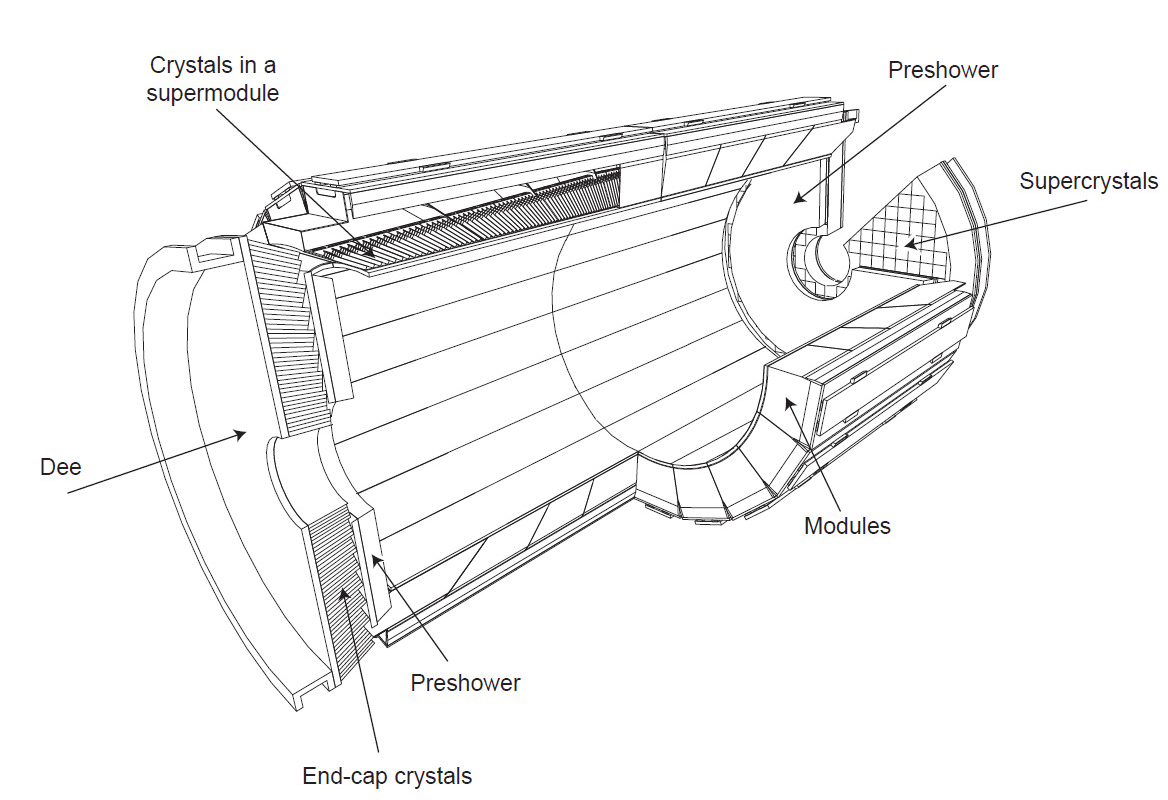
\includegraphics[width=.7\textwidth]{figures/cmsecal.png}
  \caption{The CMS electromagnetic calorimeter.}
  \label{fig:CMS_ecal}
\end{figure}

%\begin{figure}%{l}{0.5\textwidth}
%\centering
%%\includegraphics[scale=0.3]{risoluzione_ECAL.png}
%\caption{Risoluzione in energia di ECAL in funzione dell'energia del fascio di elettroni utilizzato per le misure. Sono mostrati anche i valori per i parametri di fit[16].}
%\label{fig:risoluzione_ECAL}
%\end{figure}

\noindent The energy resolution of the calorimeter is parametrized as:
\begin{equation}
{\left( \frac{\sigma}{E} \right)}^2 = {\left( \frac{S}{\sqrt{E}} \right)}^2 + {\left( \frac{N}{E} \right)}^2 + C^2,
\end{equation}
where $S=0.028 \text{ GeV}^{\frac{1}{2}}$ is the stochastic term, $N=0.12$ GeV is related to noise contribution, and $C=0.003$ is a constant term depending on the calibration.
%In figura \ref{fig:risoluzione_ECAL} sono mostrati i risultati ottenuti da misure di prova con un fascio di elettroni: le stime ottenute sono $S=0.028 \mbox{ GeV}^{\frac{1}{2}}$, $N=0.12 GeV$, $C=0.003$.


\subsection{The hadronic calorimeter}
The hadronic calorimeter (HCAL, displayed in fig.~\ref{fig:CMS_hcal}) is a sampling calorimeter, composed by brass and plastic scintillator layers. It has been designed in order to guarantee a good hermeticity, allowing to perform a precise measurement of the missing transverse energy. It is located within the electromagnetic calorimeter and the solenoid, covering a region of $|\eta|<1.3$ in the barrel, and $1.3<|\eta|<3$ in the endcaps. Brass is non-magnetic and has short interaction length (16.4 cm): the 60 mm thick absorber layers used in the barrel allow to reach 5.6 interaction lengths at $\eta=0$ and 10.8 interaction lenghts at $\eta = 1.3$; the 80 mm thick layers in the endcaps reach 11 interaction lenghts. An additional calorimetric layer has been installed out of the solenoid, in order to reach 11.8 interaction lenghts in the barrel region. The scintillation light, typically in the blue-violet region of the electromagnetic spectrum, is collected by wavalenght-shifter fibers, translated and amplified by multi-channel hybrid photodiodes, proportionally to the magnitude of the energy deposits. An additional hadronic calorimeter has been placed in the forward region, $3 < |\eta| < 5.2$, at 11.2 m from the interaction point. It has beeen designed to afford the high levels of radiations: it is composed by 55 mm thick absorber layers of stainless-steel, and quartz fibers, able to detect the Cherenkov scintillating light of the charged particles of the hadronic showering. A longitudinally segmentation allow to distinguish hadronic particles from electromagnetic components.
The energy resolution of the hadronic calorimeter is:
\begin{equation}
\left( \frac{\sigma}{E} \right) \approx \frac{a}{\sqrt{E}} \oplus b\%,
\end{equation}
where $a=65\%$ in the barrel region, $85\%$ in the endcaps, $100\%$ in the forward region, and $b=5\%$.

\begin{figure}[!htb]
  \centering
    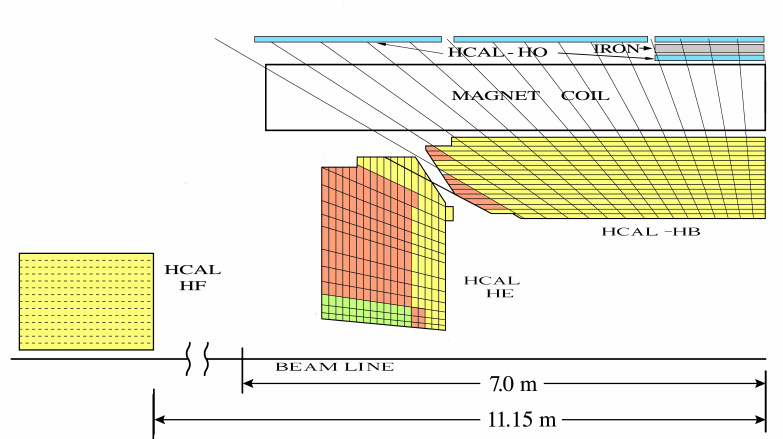
\includegraphics[width=.7\textwidth]{figures/cmshcal.png}
  \caption{The CMS hadronic calorimeter.}
  \label{fig:CMS_hcal}
\end{figure}


\subsection{The muon system}


The outer system of the CMS experiment consists into gas detectors for identifying muons, that are located between the iron return yokes, designed to close the magnetic field generated by the solenoid. In the barrel region, where a smaller number of muons is expected and the magnetic field is less strong, Drift Tubes (DT) detectors are installed. In the endcaps, where the flux of particles is larger, Cathod Strip Chambers (CSC) are used, and disposed in three disks. CSCs are designed to allow faster responses, higher granulatiy and radiation resistance. Resistive Plate Chambers (RPC) are installed both in the barrel and in the endcaps as additional triggering system. The geometry of the muon system is showed in fig.~\ref{fig:CMS_muon}; it consists of 250 DTs, 530 CSCs, 610 RPCs, and it covers a region $|\eta|<2.4$.

\begin{figure}[!htb]
  \centering
    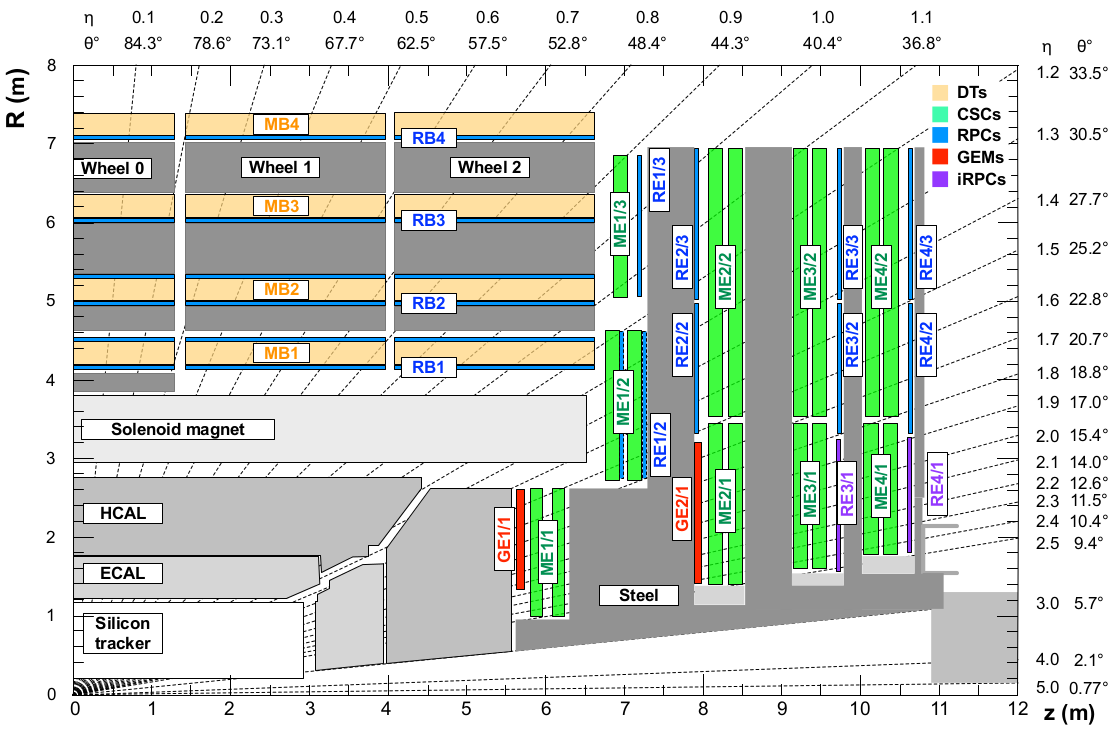
\includegraphics[width=.9\textwidth]{figures/cmsmuon.png}
  \caption{Section of CMS detector, in the plane $\mathrm{rz}$, parallel to the beamline, that emphasizes the location of the muon detectors, in particular: Drift Tubes (DT, in yellow); Cathode Strip Chambers (CSC, in green); Resistive Plate Chambers (RPC, in blue).}
  \label{fig:CMS_muon}
\end{figure}


\subsubsection{The Drift Tubes}
Drift Tube detectors cover a region of $|\eta|<1.2$ and are arranged in four stations, segmented along the beam line in five wheels. The basic element of the detector is the cell, that has a size $42 \times 13 \text{ mm}^2$. Each cell is filled with a gas mixture (85\% argon, 15\% $\text{CO}_2$), in which the process of ionization takes places; the ionization electrons drift from the 50 $\mu$m thick steel anodic wire, in the center of the cell, towards the aluminium cathodic strips, located at its edge. Additional electrodes on the surface of the cells allows to shape the electric field, in order to make the drift speed of the electrons uniform: the muon position is then extrapolated from the measurement of the drift time. Every station is composed by three cells superlayers. In the inner and the outer superlayers, the cells are oriented such in a way that the anodic wire is located along the $z$ axis, in order to measure the $\phi$ coordinate. In the intermediate superlayer, wires are parallel to the radial coordinate, hence they can measure the $z$ position. The spatial resolution of the system is 100 $\mu$m in the $r \phi$ plane, 1 mrad in the $\phi$ coordinate, and 150 $\mu$m in the longitudinal $z$ coordinate.

\subsubsection{The Cathode Strip Chambers}
Cathode Strip Chambers cover a region of $0.9<|\eta|<2.4$, overlapping with the DT in the pseudorapidity range $0.9 < |\eta| < 1.2$. The anodic wires inside each CSC are located into six planes, with the aim of measuring the radial coordinate; the wire planes are perpendicularly crossed by cathodic strips, disposed along the radial direction to measure the $\phi$ coordinate. Ionization electrons produced by muons passing through the gas mixture in the chambers migrate towards the anode, inducing a charge distribution on the cathodes, from which the azimuthal coordinate can be reconstructed. The spatial resolution in the $r$ coordinate is 200 $\mu$m, and it is 75 -- 150 $\mu$m in the $r \phi$ plane. CSCs are arranged in four disks and in three concentric rings.

\subsubsection{The Resistive Plate Chambers}
Resistive Plate Chambers (RPC) are located both in the barrel (disposed in six layers) and in the endcap region (three layers), up to a pseudorapidity of $|\eta|<1.6$. These gas detectors are charged at very high voltages, in order to work in the avalanche ionization mode. The plastic resitive plates are equipped with readout strips. The spatial resolution of the detector is low (1-2 cm), but the fast timing response (2-3 ns) and good time resolution (1 ns) allow to employ RPCs as an additional triggering system and to profit of a precise measurement of the bunch-crossing time.

%\subsection{Other CMS sub-detectors}
%Tracciatori e camere per i muoni coprono una regione di $|\eta|<2.5$, gli apparati calorimetrici arrivano fino ad $|\eta|<5.2$. Ci sono altri due rivelatori che permettono misure nella regione $5 \leq |\eta| \leq 11$, TOTEM e CASTOR. TOTEM sfrutta dei rivelatori a gas per le misure di scattering elastico protone protone in funzione del loro momento. CASTOR \`e un calorimetro elettromagnetico ed adronico che raccoglie luce Cherenkov, serve per misure di QCD in collisioni p-p, p-ione, ione-ione.

\subsection{The trigger system and data acquisition}
The CMS trigger system has been designed considering the high instantaneous luminosity, such that it can provide a fast response and it allows to reduce the nominal event rate of 40 MHz in proton proton collision. The complexity of the CMS detector and the very high number of readout channels result into a huge amount of data per event, approaching the order of few MB per bunch crossing, hence 40 TB per second. The handling and the recording of data is currently limited at the order of $\sim$100 Hz; hence, applying online selections to skim the events that are going to be written on tape, without rejecting interesting signals of hard processes and rare phenomena becomes a crucial and challenging point for every data analysis. Events are filtered by trigger selections at different levels: the Level-1 (L1) trigger is an hardware device, that allows to reduce the event rate from 40 MHz to the order of 100 kHz; the High Level Trigger (HLT) is a set of software algorithms that skims the event rate down to few hundred Hz. Once the trigger decisions are taken, the final events are handled by the Data Acquisition System (DAQ), that collects the informations coming from to the subdetectors and sends them to the storage devices.

\subsubsection{The Level-1 trigger}
The L1 trigger is an hardware device composed by customized electronics, and it accesses the informations coming from the calorimeters and the muon system, while the tracker is not considered given the excessively large bandwidth needed by its readout channels. The L1 trigger perform a first raw local reconstruction of each object, called ``trigger primitive''. The L1 trigger is composed by three subsystems: the calorimeter trigger, the muon trigger (divided in three independent sub-subsystems for each muon subdetector, namely DTs, RPCs and CSCs), and the global trigger, that combines the informations of the former subsystems. The best quality trigger primitives reconstructed by the calorimeter and muon detectors (namely, roughly reconstructed electrons, photons, muons, jets, jets coming from the hadronic decays of tau leptons, and missing energy) are handled by the global trigger, who takes the decision of discarding or keeping the event every 3.2 $\mu$s. The simplest trigger selections require the presence of a single object, whose energy or transverse momentum is higher than a certain threshold; more complicated triggers involve multiple objects or geometrical selections, that can be performed in parallel up to 128 simultaneous requirements.

\subsubsection{The High Level Trigger}
The HLT skims the L1 output rate down to few hundreds of Hz by applying a set of algorithms implemented in the same software used for the offline analysis, consisting in the event reconstructions exploiting the whole informations coming from all subdetectors. The computing time is still a crucial factor, hence selections applied to HLT physics objects are generally less accurate than those of the offline analysis; furthermore, HLT can discard the event even before its full reconstruction (\textit{i.e.} by looking only at certain region of the detectors). Events filtered by the HLT decisions are assigned to precise trigger paths and recorded in precise categories of datasets.

\subsubsection{Data acquisition, computing and storage}
The DAQ system deals with the storage, transfer and handling of the data collected by CMS; it also supports and stores the data simulations and calibrations of the subdetectors. The CMS computational resources are located in worldwide distributed data nodes, called Tiers. The CMS software (CMSSW) is based on an object oriented architecture (mainly C++). The basic unity of every data, both real and simulated ones, is the Event, that could contain very rough informations (RAW data format) or higher level refined objects (AOD, Analysis Object Data) where all the calibrations and corrections needed to properly deal with the final physics objects are already in place. Data are handled by C++ or python modules, and the outputs are written in ROOT files. [citazione]

\subsection{Particle Flow event reconstruction}
-- ref from paper
The global event reconstruction at CMS relies on the particle flow (PF) [69, 70] algorithm, which
reconstructs and identifies each individual particle with an optimized combination of informa-
tion from the various elements of the CMS detector. The energy of photons is directly obtained
from the ECAL measurement, while the energy of electrons is determined from a combina-
tion of the electron momentum at the primary interaction vertex as determined by the tracker,
the energy of the corresponding ECAL cluster, and the energy sum of all bremsstrahlung pho-
tons spatially compatible with originating from the electron track. The momentum of muons
is obtained from the curvature of the corresponding track. The energy of charged hadrons is
determined from a combination of their momentum measured in the tracker and the match-
ing ECAL and HCAL energy deposits, and the energy of neutral hadrons is obtained from the
corresponding ECAL and HCAL energy.
The core of the particle flow reconstruction technique is the algorithm used to link the signals
of the individual subdetectors. The association criteria is purely geometrical. The aim is a
full reconstruction of each single particle, while reducing any possible double counting from
different detectors. Given the granularity of the calorimeters, energy deposits and tracks are
linked if their trajectory intersects one of the calorimetric cells, and likewise clusters in the
ECAL pre-shower, ECAL and HCAL are linked if the cluster position is compatible in the η, φ
plane between the extrapolated track position and the cluster position.


The particle-flow event reconstruction aims at reconstructing and identifying all sta-
ble particles in the event, i.e. electrons, muons, photons, charged hadrons and neu-
tral hadrons, by mean of an optimized combination of informations from all CMS sub-
detectors. The algorithm is described in detail in References [44–46] where information
on its commissioning with early data are also provided. The CMS PF algorithm relies
on a efficient and pure track reconstruction, on a clustering algorithm able to disentangle
overlapping showers, and on an efficient link procedure to connect together the deposits
of each particle in the sub-detectors. Tracks are extrapolated through the calorimeters: if
they fall within the boundaries of one or several clusters, the clusters are associated to
the track. The set of track and cluster(s) constitute a charged hadron and are not con-
sidered anymore in the rest of the algorithm. The muons are identified beforehand so
that their track does not give rise to a charged hadron. The electrons are more difficult to
deal with. Indeed, due to the frequent Bremsstrahlung photon emission, a specific track
reconstruction (the GSF already discussed in Section 2.2.3.1) is needed as well as a ded-
icated treatment to properly attach the photon clusters to the electron and avoid energy
double counting. Once all the tracks are treated, the remaining clusters result in photons
in case of the electromagnetic calorimeter (ECAL), and in neutral hadrons in the case a
hadron calorimeter (HCAL) cluster is matched to an ECAL cluster. Once all the deposits
of a particle are associated, its nature can be assessed, and the information of the sub-
detectors combined to determine optimally its four-momentum. In case the calibrated
calorimeter energy of the clusters, which is simply a linear combination of the ECAL and
HCAL energy deposits, associated to a track is found to be in excess with respect to the
track momentum at more than one sigma, the excess is attributed to an overlapping neu-
tral particle (photon or hadron), carrying an energy corresponding to the difference of
the two measurements. The resulting list of particles, namely charged hadrons, photons,
neutral hadrons, electrons and muons, is then used to reconstruct the jets, the missing
transverse energy, to reconstruct and identify the τ from their decays products and to
measure the isolation of the particles.
The association used in the linking stage is purely geometrical: tracks are linked to calori-
metric clusters if their trajectory intersects one of the calorimetric cells of the cluster; and
likewise clusters in the ECAL preshower, ECAL and HCAL are linked if the cluster posi-
tion measured in the finer granularity subdetector lies within the envelop of the cluster 
in the coarser granularity subdetector. In order to account for uncertainties from mul-
tiple scattering in the track extrapolation and on the estimated position of the shower
maximum in the calorimeters, a geometrical tolerance of the size of one calorimeter cell
is included when defining links; this tolerance can also account for gaps and cracks in
the calorimeters. By design, the linking algorithm is simple and robust, as it does not
rely on the precise knowledge of the position resolution in each subdetector. Special-
ized algorithms are used for linking tracks to recover bremsstrahlung clusters in the
case of electrons by considering tangents to electron trajectories at the crossing points
with the tracker layers. Blocks of one or more linked objects are then processed to iden-
tify and reconstruct particle candidates. Isolated electrons and muons are selected first,
and reconstructed using the dedicated algorithms developed for them; similarly, non-
isolated tracks which satisfy tight muon identification criteria are immediately identi-
fied as muons. Charged hadrons are identified as tracks in the inner tracker, normally
linked to calorimetric deposits if the particle p T is sufficient for the trajectory to reach the
calorimeters. If the momentum measurements from the track and calorimeter are com-
patible, after accounting for non-linearities and zero suppression effects, the best energy
determination is obtained as a combination of the two. If the track momentum signif-
icantly exceeds the measured calorimetric energy, the particle is identified as muon if
it satisfies very loose muon identification criteria; otherwise, tight track quality require-
ments are applied to to reject mis-reconstructed tracks. If instead an excess of calorimetric
energy deposition is found with respect to the momentum of the associated track, e.g. in
the case of collimated hadronic jets, the residual energy is identified as a photon or a neu-
tral hadron. Additional photons and neutral hadrons are also identified from calorimetric
deposits not linked to any track.
\subsection{Physics objects}

\subsubsection{Track and vertex reconstruction}
\subsubsection{Electron reconstruction}
\subsubsection{Photon reconstruction}
\subsubsection{Muon reconstruction}
L'intero sistema misura in maniera ``standalone'' l'impulso con una risoluzione in $p_T$ di circa $\Delta p_T/p_T \approx 8-15\%$ per muoni di $p_T = 10$ GeV/c e di $\Delta p_T/p_T \approx 20-40\%$ per muoni di $p_T = 1$ TeV/c. Combinando con la misura nei rivelatori al silicio la risoluzione passa rispettivamente all'$1\%$ e al $7-16\%$.\\
\subsubsection{Jet reconstruction}
\subsubsection{Tau reconstruction}
\subsubsection{Missing transverse energy reconstruction}
\subsubsection{b-quark tagging}


\section{ATLAS, ALICE, LHCb detectors}

\subsection{ATLAS}
ATLAS (A Toroidal LHC ApparatuS) is a multi-purpose experiment, that shares the same scientifical aims of CMS. The simultaneous observation of an Higgs boson-like particle at the two experimental facilities represented an irrefutable proof of the discovery of the Higgs boson.\\
ATLAS has a cylindrical shape (diameter of 25 m, length of 46 m) and weights 7000 tons. Like CMS, ATLAS is composed by many sub-detectors: trackers, calorimeters and muon system. The ATLAS magnetic field is provided by a solenoid, located inside the cylinder, and a big toroid, located outside the sub-detectors, able to reach a magnetic field of 2 T at the interaction point. The main differences among the two experiments are listed below.

\begin{itemize}
\item {\itshape Tracker --} the CMS tracker has a better $p_T$ resolution (mainly due to the higher magnetic field): $\sigma_{p_T}/p_T \approx 5 \cdot 10^{-4} p_T + 0.01$ at ATLAS; $\sigma_{p_T}/p_T \approx 1.5 \cdot 10^{-4} p_T + 0.005$ at CMS.
\item {\itshape Electromagnetic calorimeter --} the CMS electromagnetic calorimeter is completely enclosed inside the solenoid, whilst ATLAS calorimeter is outside of the solenoid. The particles going through the solenoid suffer an energy loss and a consequent deterioration of the energy resolution. The CMS ECAL has an enery resolution of $\sigma_E /E \approx 3\%/\sqrt{E}$; the ATLAS calorimeter has a sandwich structure (liquid argon and lead layers) and a resolution of $\sigma_E / E \approx 10\%/\sqrt{E}$.
\item {\itshape Hadronic calorimeter --} the CMS HCAL is partly inside the solenoid, partly outside, depauperating the resolution. The ATLAS hadronic calorimeter (made of iron and plastic scintillator tiles) has an energy resolution $\sigma_E /E \approx 50\%/\sqrt{E} + 0.03$ GeV; CMS HCAL has a resolution of $\sigma_E /E \approx 100\%/\sqrt{E} + 0.05$ GeV.
\item {\itshape Muon system --} the peculiar geometry of the ATLAS muon system allows a better resolution of the standalone measurement of the muon momenta (\textit{i.e.}, without using tracker and calorimeters), that is around 10\% at 1 TeV. CMS has better performance when combining the informations coming from the inner detectors (7\% at 1 TeV against the 35\% for the standalone measurement).
\end{itemize}

\subsection{ALICE}
ALICE (A Large Ion Collider Experiment) studies the heavy ion collisions (lead-lead) or proton-ion in order to explore the physics of the hadrons in high density (or temperature) regimes, when a new state of matter appears, the so-called quark-gluon plasma (QGP). The QGP played a crucial role in the very first instants of life of the universe.

\subsection{LHCb}
LHCb (Large Hadron Collider beauty) is a detector designed to study the b quark properties, in particular the CP violation and other rare phenomena involved in b hadrons. The final aim of these measurements is trying to solve the matter-antimatter asymmetry problem.

\vspace*{1\baselineskip}

\noindent The three detectors are depicted in fig.~\ref{fig:ATLAS}--\ref{fig:LHCb}.


\begin{figure}%{l}{0.5\textwidth}
\centering
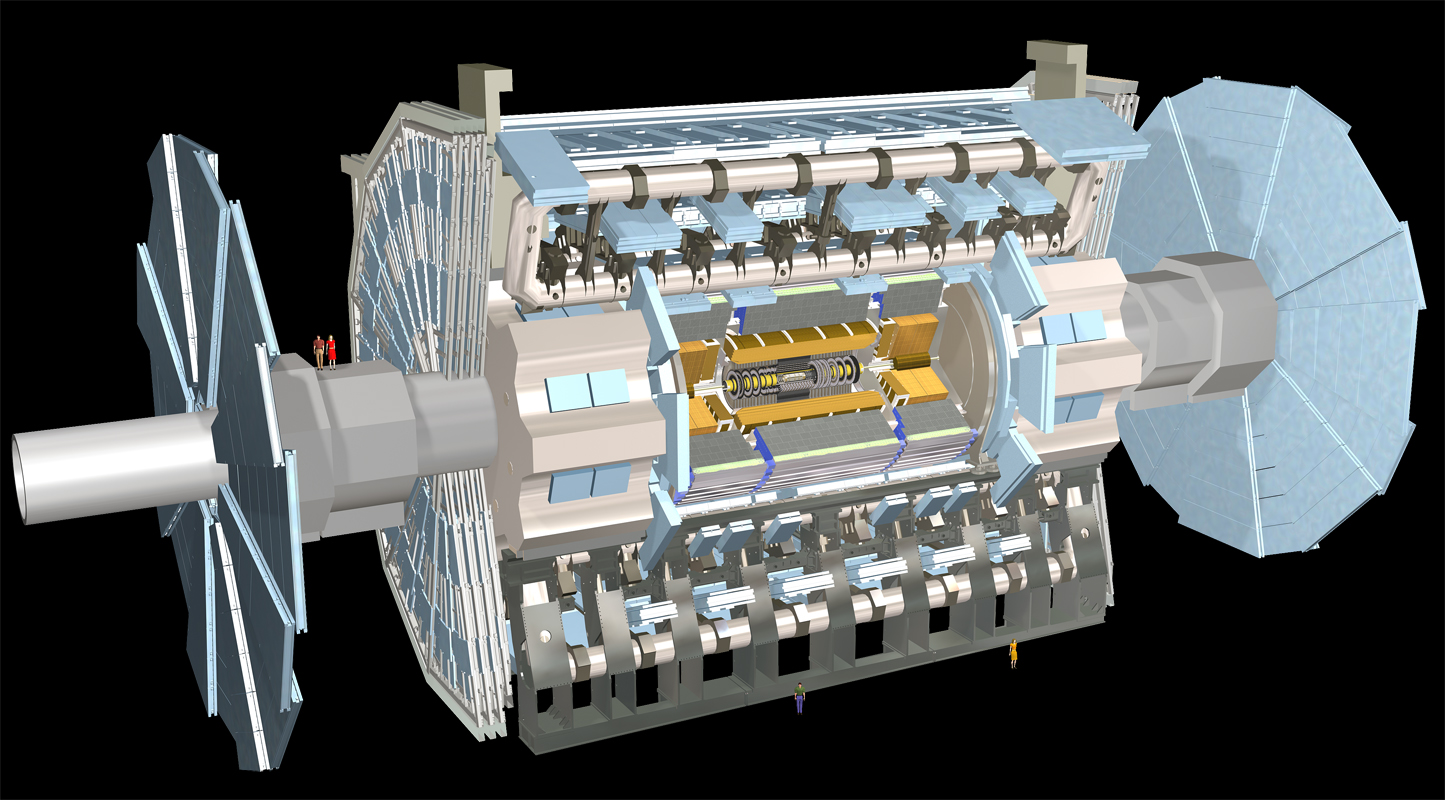
\includegraphics[width=.6\textwidth]{figures/ATLAS.jpg}
\caption{The ATLAS experiment.}
\label{fig:ATLAS}
\end{figure}

\begin{figure}%{l}{0.5\textwidth}
\centering
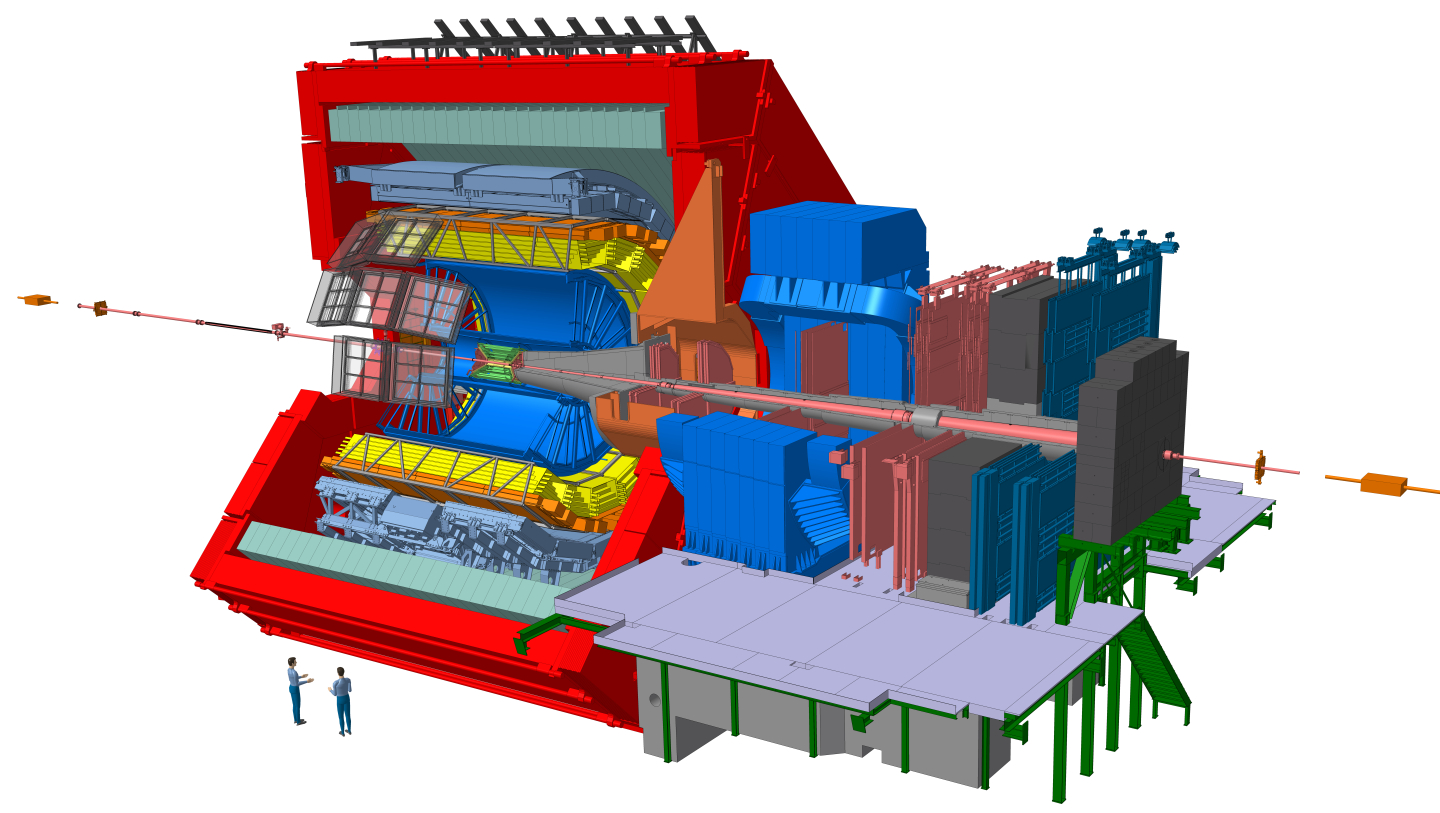
\includegraphics[width=.6\textwidth]{figures/ALICE.jpg}
\caption{The ALICE experiment.}
\label{fig:ALICE}
\end{figure}

\begin{figure}%{l}{0.5\textwidth}
\centering
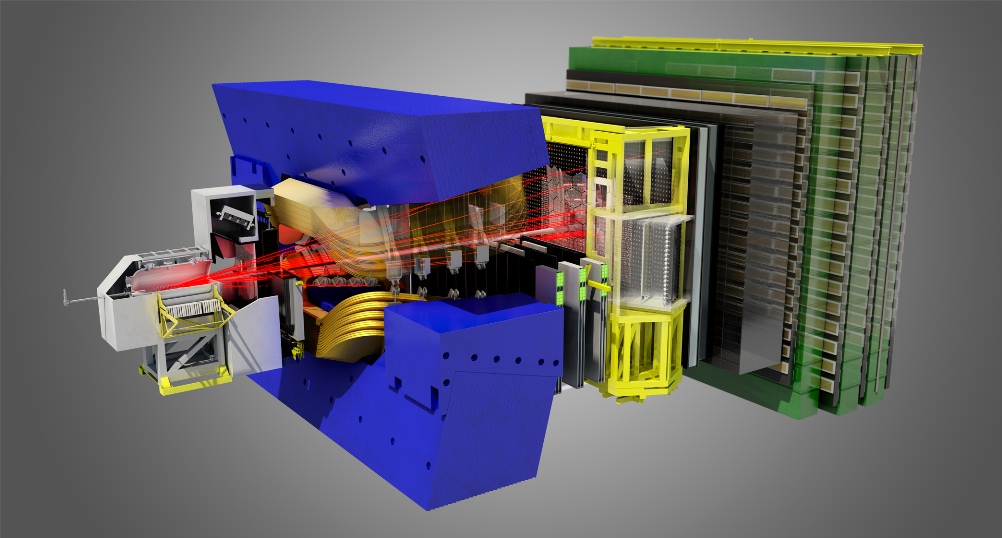
\includegraphics[width=.6\textwidth]{figures/LHCb.png}
\caption{The LHCb experiment.}
\label{fig:LHCb}
\end{figure}

\clearpage


\section{Analysis overview}
\label{sec:analysis_overview}

%Many diboson analyses are being performed with Run 2 2016 data by CMS collaboration, covering a plethora of different final states. In this thesis, a search for diboson resonances in the $\nu \bar{\nu} q \bar{q}$ is performed. 
This analysis searches for potential signals of heavy resonances decaying into a pair of vector bosons, using the data collected by the CMS experiment during 2016, corresponding to an integrated luminosity of $\mathcal{L}=35.9 \mbox{ fb}^{-1}$. One of the boson should be a \Z, and it is identified through its invisible decay into a couple of neutrinos ($\nu \bar{\nu}$), while the other electroweak boson, labelled as \V and consisting either in a \W or in a \Z boson, is required to decay hadronically into a pair of quarks ($q \bar{q}$). %The final states probed by this analysis therefore consists in two quarks and two neutrinos, reconstructed as missing transverse energy (\met).
The decay products (the bosons) of heavy (around the TeV scale) resonances are produced with large Lorentz boosts; as a consequence, the decay products of the bosons (quarks and neutrinos) are expected to be highly energetic and collimated. In this regime, the standard jet reconstruction algorithms fail in distinguishing the two jets from the quarks, suggesting to look for a signature composed of a large-cone high-\pt jet, in which both $q$ and $\bar{q}$ lie, recoiling against a large amount of missing transverse momentum (\met) due to the neutrinos escaping the detector. The hadronically decaying boson ($Z$, $W$) is then reconstructed as one large-cone jet, whose mass is used to define the signal region and signal-depleted control regions, the sidebands. %Jet substructure techniques are exploited in order to suppress background contamination and to classify the events in two exclusive signal purity categories, allowing to improve the discovery reach.
The analysis of the jet substructure improves the background suppression and it allows to group the events in two mutually exclusive categories, with different signal purity, enhancing the sensitivity of the search.

\noindent A general $ZZ$ decay, predicted by the bulk graviton model (sec.~\ref{sec:BG}), can be reconstructed both in final states with high signal purity but limited statistics (four charged leptons) and large statistics but overwhelming backgrounds (no charged leptons). The choice to look for one boson decaying hadronically and the other $Z$ into neutrinos represents the best compromise between these two extremes. This topology can be also utilized to reconstruct a charged spin-1 vector boson \Wp decaying into an invisible $Z$ and an hadronic $W$, predicted by the HVT model (sec.~\ref{sec:theory_HVT}), making this analysis sensitive to a generic \VZ final state.

\noindent Signal events are collected with trigger paths requiring high \met recoiling against jet activity. This signature is clearly a very challenging one in an environment with more than 50 primary collisions per bunch crossing. For this reason, the Particle-Flow algorithm is run at trigger level to obtain the highest possible resolution on the jets and thus on the \met.

\noindent The search is performed by examining the distribution of the diboson reconstructed transverse mass of the resonance \VZ (\mtVZ) for a localized excess. The shape and normalization of the main background of the analysis (namely, the production of an electroweak boson in association with jets) are estimated with a data-simulation hybrid approach using the distribution of data in the sidebands, corrected for a function accounting for potential differences between the signal region and the sidebands. The predictions of the secondary background sources completely rely on simulations.

\noindent In fig.~\ref{fig:event_display}, a typical signal event of the \Wpinv process, reproduced with a realistic simulation of the CMS detector, is displayed; the mass of the \Wp is 2.5 TeV. The muon chambers in the barrel (DTs, in light red) and in the endcaps (CSCs, in light blue), along with the tracker detector (green) are shown in the $(r, \varphi)$ transverse plane (left) and the $(r, z)$ longitudinal plane (right). The large-cone jet, identifying the \W hadronic decay, is displayed in red; the energy deposits in ECAL (light orange) and in HCAL (in violet) can be seen in the pictures. The missing transverse energy, signature of the \Z invisible decay, is represented as a blue arrow, lying in the transverse plane. %The track multiplicity (green tracks) is shown in the center of the detector, where the tracker is installed.
Green tracks represent charged particles from the underlying events as reconstructed by the silicon tracker.

\begin{figure}[!htb]
  \centering
    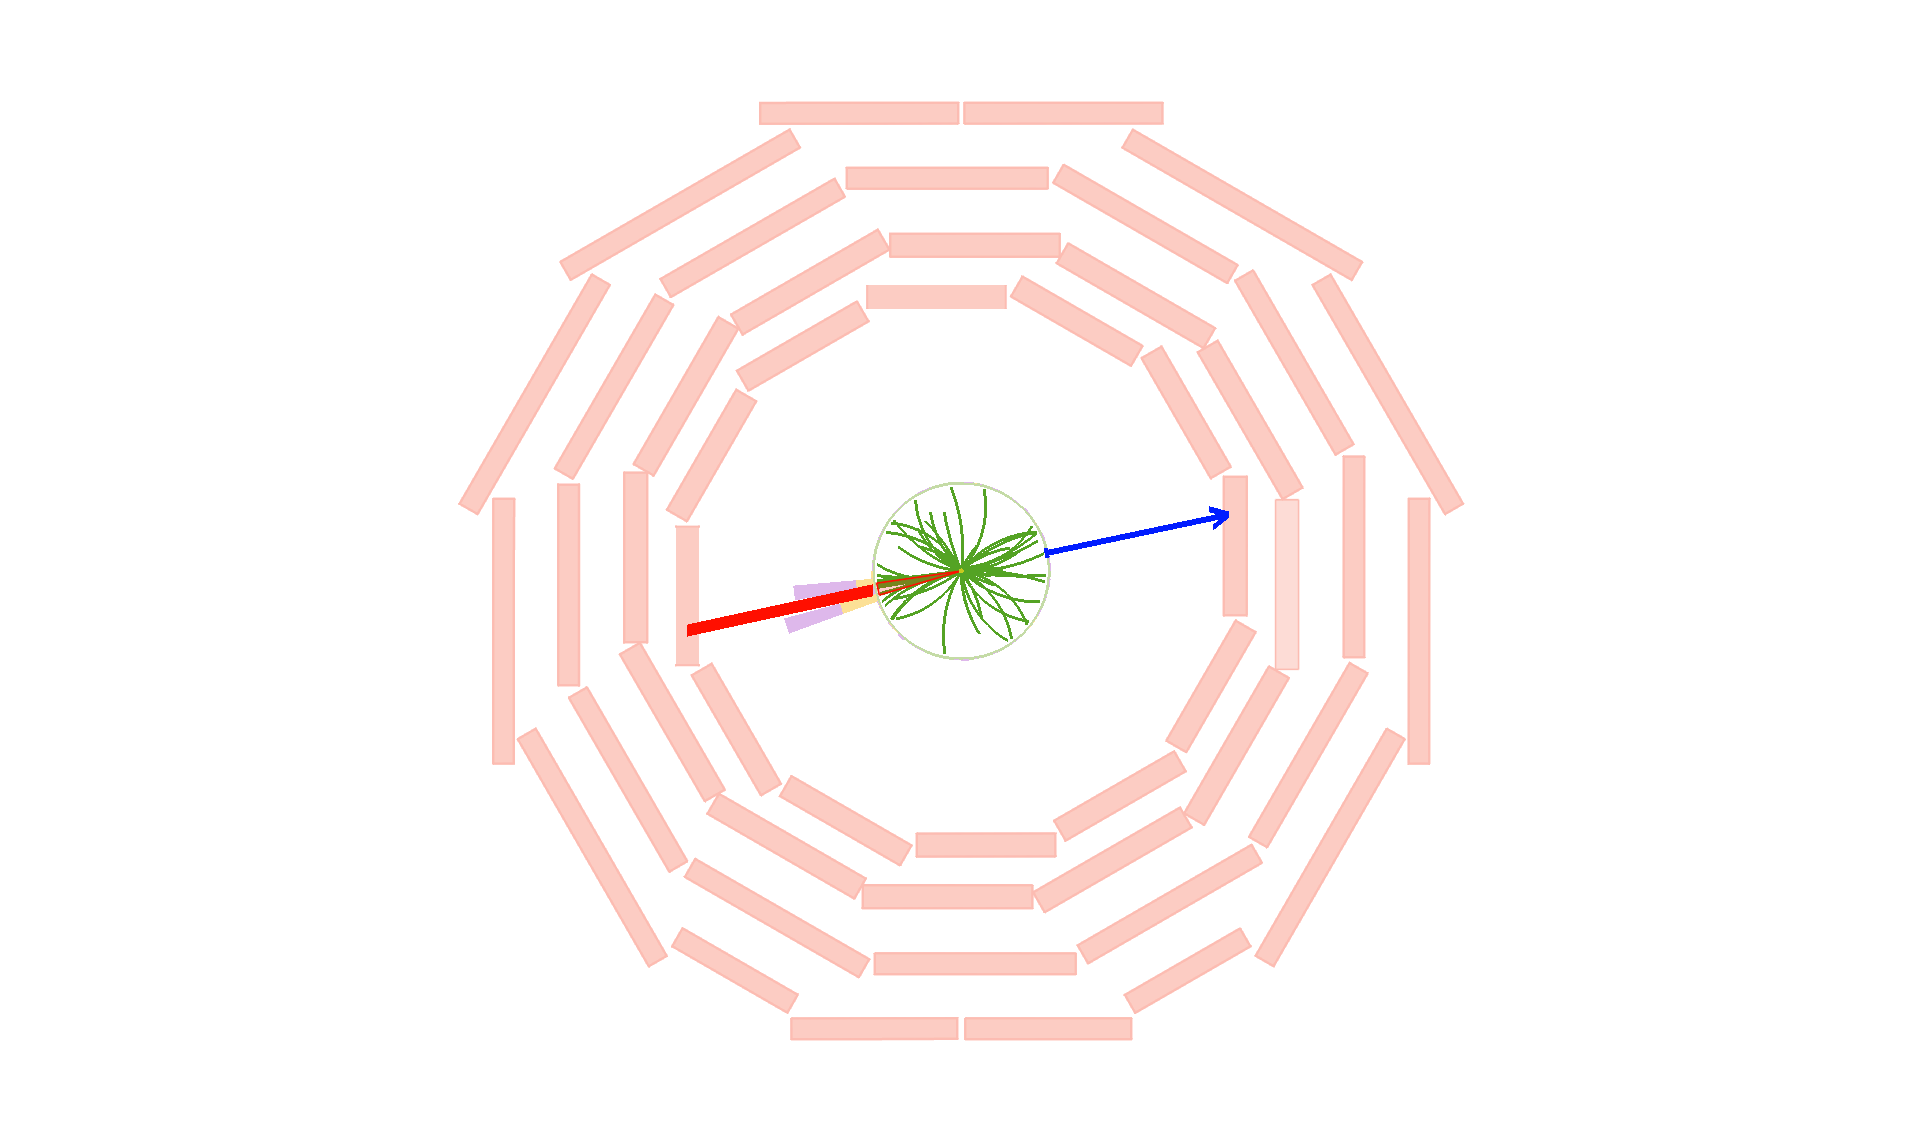
\includegraphics[width=.5\textwidth]{evdisp/Wprime25Tev_rhophi_all.png}%
    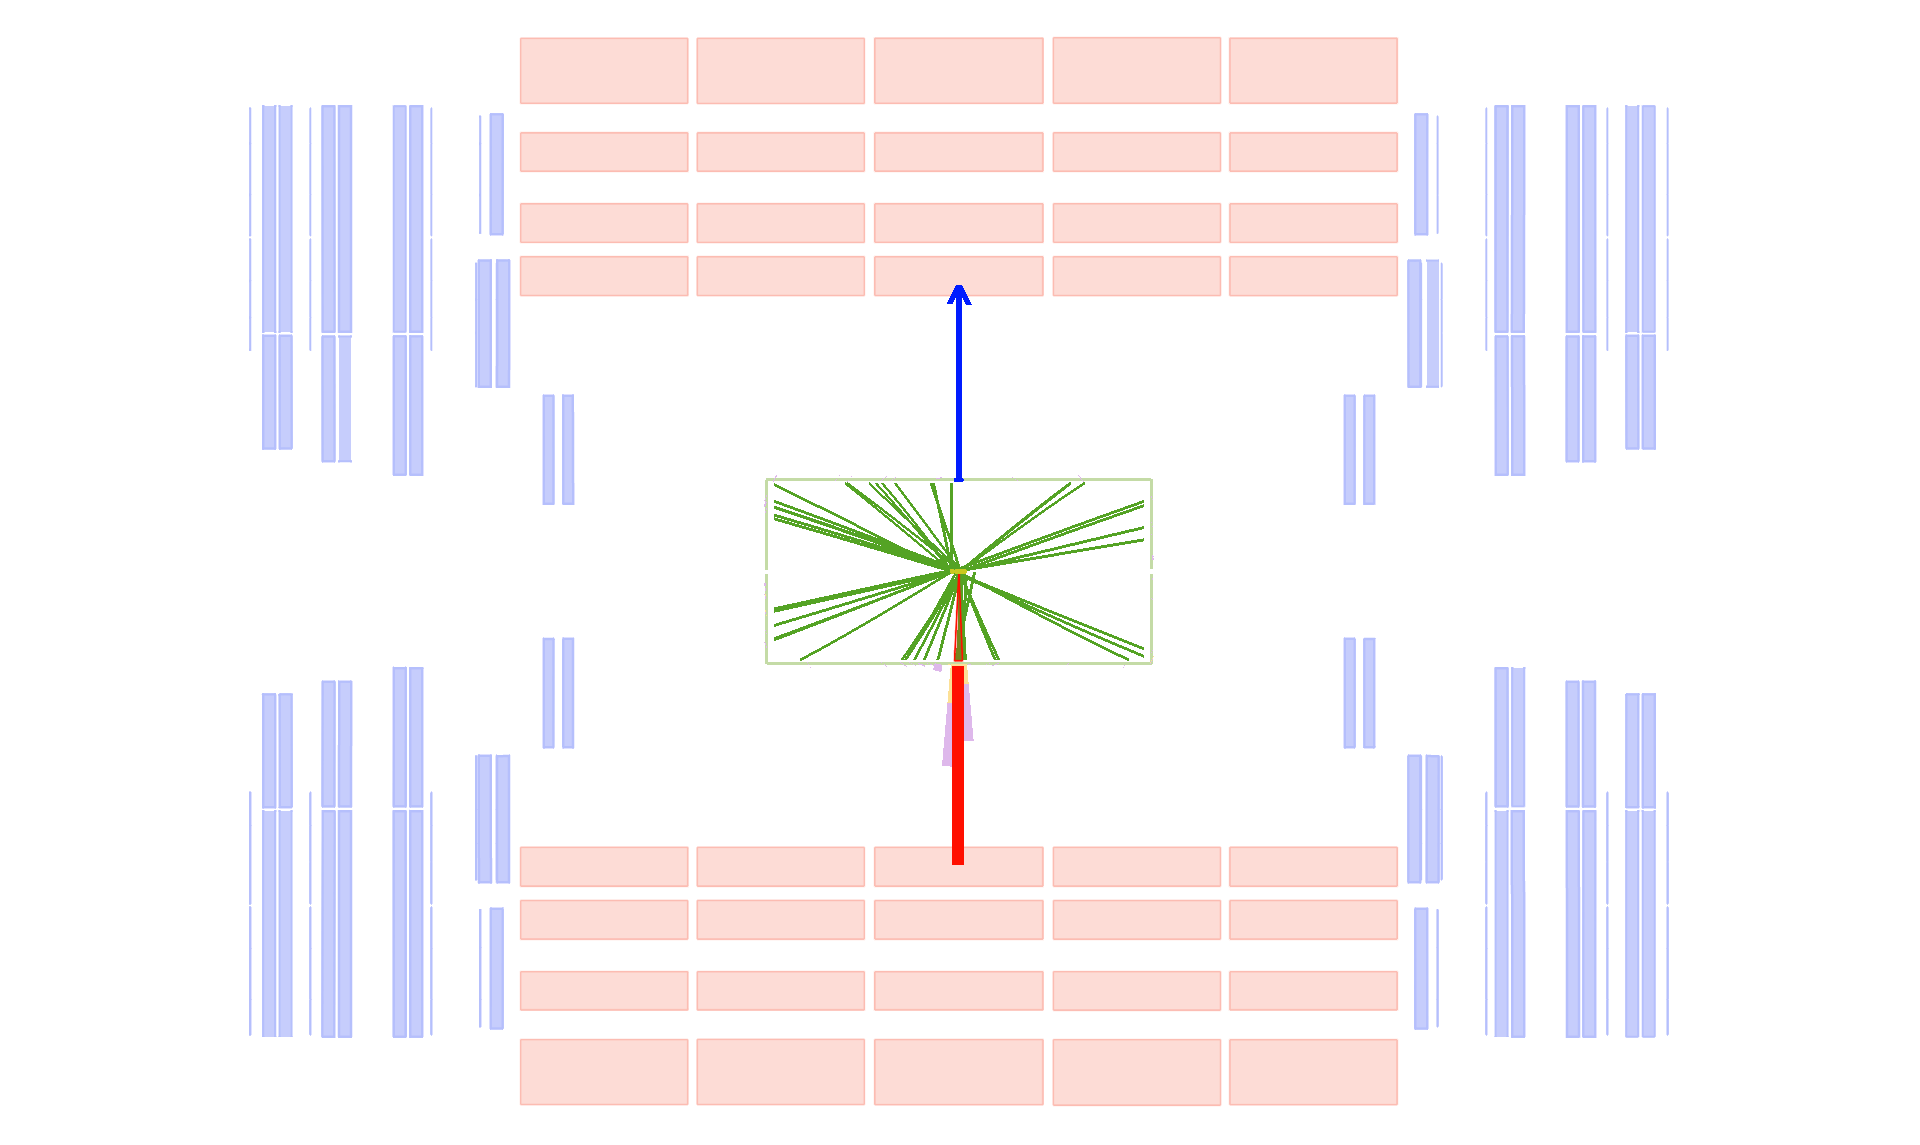
\includegraphics[width=.5\textwidth]{evdisp/Wprime25Tev_rhoz_all.png}%

  \caption{Left: representation of the decay of a \Wp of mass 2.5 TeV, in the transverse plane of the CMS detector. Right: representation of the same event, in the longitudinal plane of the CMS detector.}
  \label{fig:event_display}
\end{figure}


%\section{Data and Monte Carlo simulations samples}
%\begin{tcolorbox}[breakable,colback=black!5!white,colframe=red!80!black,width=\textwidth]
%\chapter*{Data and Monte Carlo samples}
%\end{tcolorbox}
\label{chap:samples}

\subsection{Signal samples}

Signal samples of a spin-2 (Bulk Graviton) decaying in a pair of \Z bosons are exploited in the analysis. To target the final state, one of the two \Z bosons is forced to decay into neutrinos, while the other \Z is forced to decay hadronically. The signal samples are produced in the narrow-width approximation by setting the resonance with to 0.1\% of its mass. Twelve mass points with 100000 events each are simulated, with a $m_{\G}$ ranging from 600 \GeV up to 4500 \GeV.

\noindent Additionally, samples of a spin-1 HVT-like \Wp resonance decaying in a \Z boson and a \W boson are studied. The \Z boson is forced to decay into neutrinos, and the \W boson is forced to decay hadronically. Also in this case the signal samples are produced in the narrow-width approximation by setting the resonance with to 0.1\% of its mass. Twelve mass points with 100000 events each are simulated, with a $m_{\Wp}$ ranging from 600 \GeV up to 4500 \GeV.

\noindent The signal samples are generated at leading-order (LO) with the {\sc MadGraph5\_aMCatNLO v 2.2.2}~\cite{bib:MADGRAPH} matrix element generator, while hadronization and fragmentation are handled by \PYTHIA 8~\cite{bib:PYTHIA} version 8.2121 with CUETP8M1~\cite{bib:CUETP8M1} tuning. A full detector simulation and event reconstruction has been performed with \GEANTfour~\cite{bib:GEANT4} and CMSSW. The detector alignement scenario, calibrations and pile-up distributions are generated according to the expectations in 2016 data.
%All signal samples belong to the {\tt RunIISummer16MiniAODv2\_PUMoriond17-80X\_mcRun2} campaign.

\noindent All the signal samples used in the analysis and the related properties are reported in Tables~\ref{tab:signal_samples}-\ref{tab:signal_samples_W}.
%Missing W'
%and ~\ref{tab:signal_samples_W}. 
 
 \begin{table}[!htb]
   \begin{center}
   \begin{tabular}{lccc}
 Signal process &  $m_{\G}$ & Events & $\sigma\times\mathcal{B}$ (\pb) \\
 \hline 
\BGinv & 600 GeV & 100000 & 0.27964\\
\BGinv & 800 GeV  & 100000 & 0.27964\\
\BGinv & 1000 GeV  & 100000 & 0.27964\\
\BGinv & 1200 GeV  & 100000 & 0.27964\\
\BGinv & 1400 GeV  & 100000 & 0.27964\\
\BGinv & 1800 GeV  & 100000 & 0.27964\\
\BGinv & 2000 GeV  & 100000 & 0.27964\\
\BGinv & 2500 GeV  & 100000 & 0.27964\\
\BGinv & 3000 GeV  & 100000 & 0.27964\\
\BGinv & 3500 GeV  & 100000 & 0.27964\\
\BGinv & 4000 GeV  & 100000 & 0.27964\\
\BGinv & 4500 GeV  & 100000 & 0.27964\\
   \end{tabular}
   \end{center}
   \caption{Spin-2 (Bulk Graviton) signal samples and production cross sections (assumed to be $1\pb$) multiplied by the respective branching fractions of the \Z decays considered ($\mathcal{B}(\Z \to \nu\nu) = 0.20$, $\mathcal{B}(\Z \to qq) = 0.6991$). \label{tab:signal_samples}}
 \end{table}

 \begin{table}[!htb]
   \begin{center}
   \begin{tabular}{lccc}
 Signal process &  $m_{\Wp}$ & Events & $\sigma\times\mathcal{B}$ (\pb) \\
 \hline
\Wpinv & 600 GeV & 100000 & 0.13482\\
\Wpinv & 800 GeV  & 100000 & 0.13482\\
\Wpinv & 1000 GeV  & 100000 & 0.13482\\
\Wpinv & 1200 GeV  & 100000 & 0.13482\\
\Wpinv & 1400 GeV  & 100000 & 0.13482\\
\Wpinv & 1800 GeV  & 100000 & 0.13482\\
\Wpinv & 2000 GeV  & 100000 & 0.13482\\
\Wpinv & 2500 GeV  & 100000 & 0.13482\\
\Wpinv & 3000 GeV  & 100000 & 0.13482\\
\Wpinv & 3500 GeV  & 100000 & 0.13482\\
\Wpinv & 4000 GeV  & 100000 & 0.13482\\
\Wpinv & 4500 GeV  & 100000 & 0.13482\\
   \end{tabular}
   \end{center}
   \caption{Spin-1 (W') signal samples and production cross sections (assumed to be $1\pb$) multiplied by the \Z and \W branching fraction ($\mathcal{B}(\Z \to \nu\nu) = 0.2$, $\mathcal{B}(\W \to qq) = 0.6760$).\label{tab:signal_samples_W}}
 \end{table}


\subsection{Signal characterization}

This analysis is performed in a high mass region (from 1~\TeV to 4.5~\TeV). The \MADGRAPH algorithm generates the hard process production in the collision with \pt = 0. In the next step of the simulation, during the hadronization, \PYTHIA adds the QCD ISR (initial state radiation) and consequently a resonance \pt different from 0.
%The transverse mass and \pt distributions of the heavy resonance after the \PYTHIA simulation are shown in fig.~\ref{fig:genSignal1} for Bulk Graviton signal samples (and in fig.~\ref{fig:genSignal2} for \Wp signal samples). The typical \pt is small compared to the mass of the resonance, and about two thirds of the events have \pt smaller than 50 \GeV. The \pt distributions of the electroweak bosons, along with the mass of the hadronically decaying \Z (\W) and the angular separation of the two electroweak bosons in the transverse plane are shown as well.
Kinematical distributions at generator level are showed in fig.~\ref{fig:genGravSignal1}-\ref{fig:genGravSignal3} for spin-2 Bulk Graviton signal, and in fig.~\ref{fig:genWprimeSignal1}-\ref{fig:genWprimeSignal3} for spin-1 HVT \Wp signal.

 \begin{figure}[!htb]
   \begin{center}
     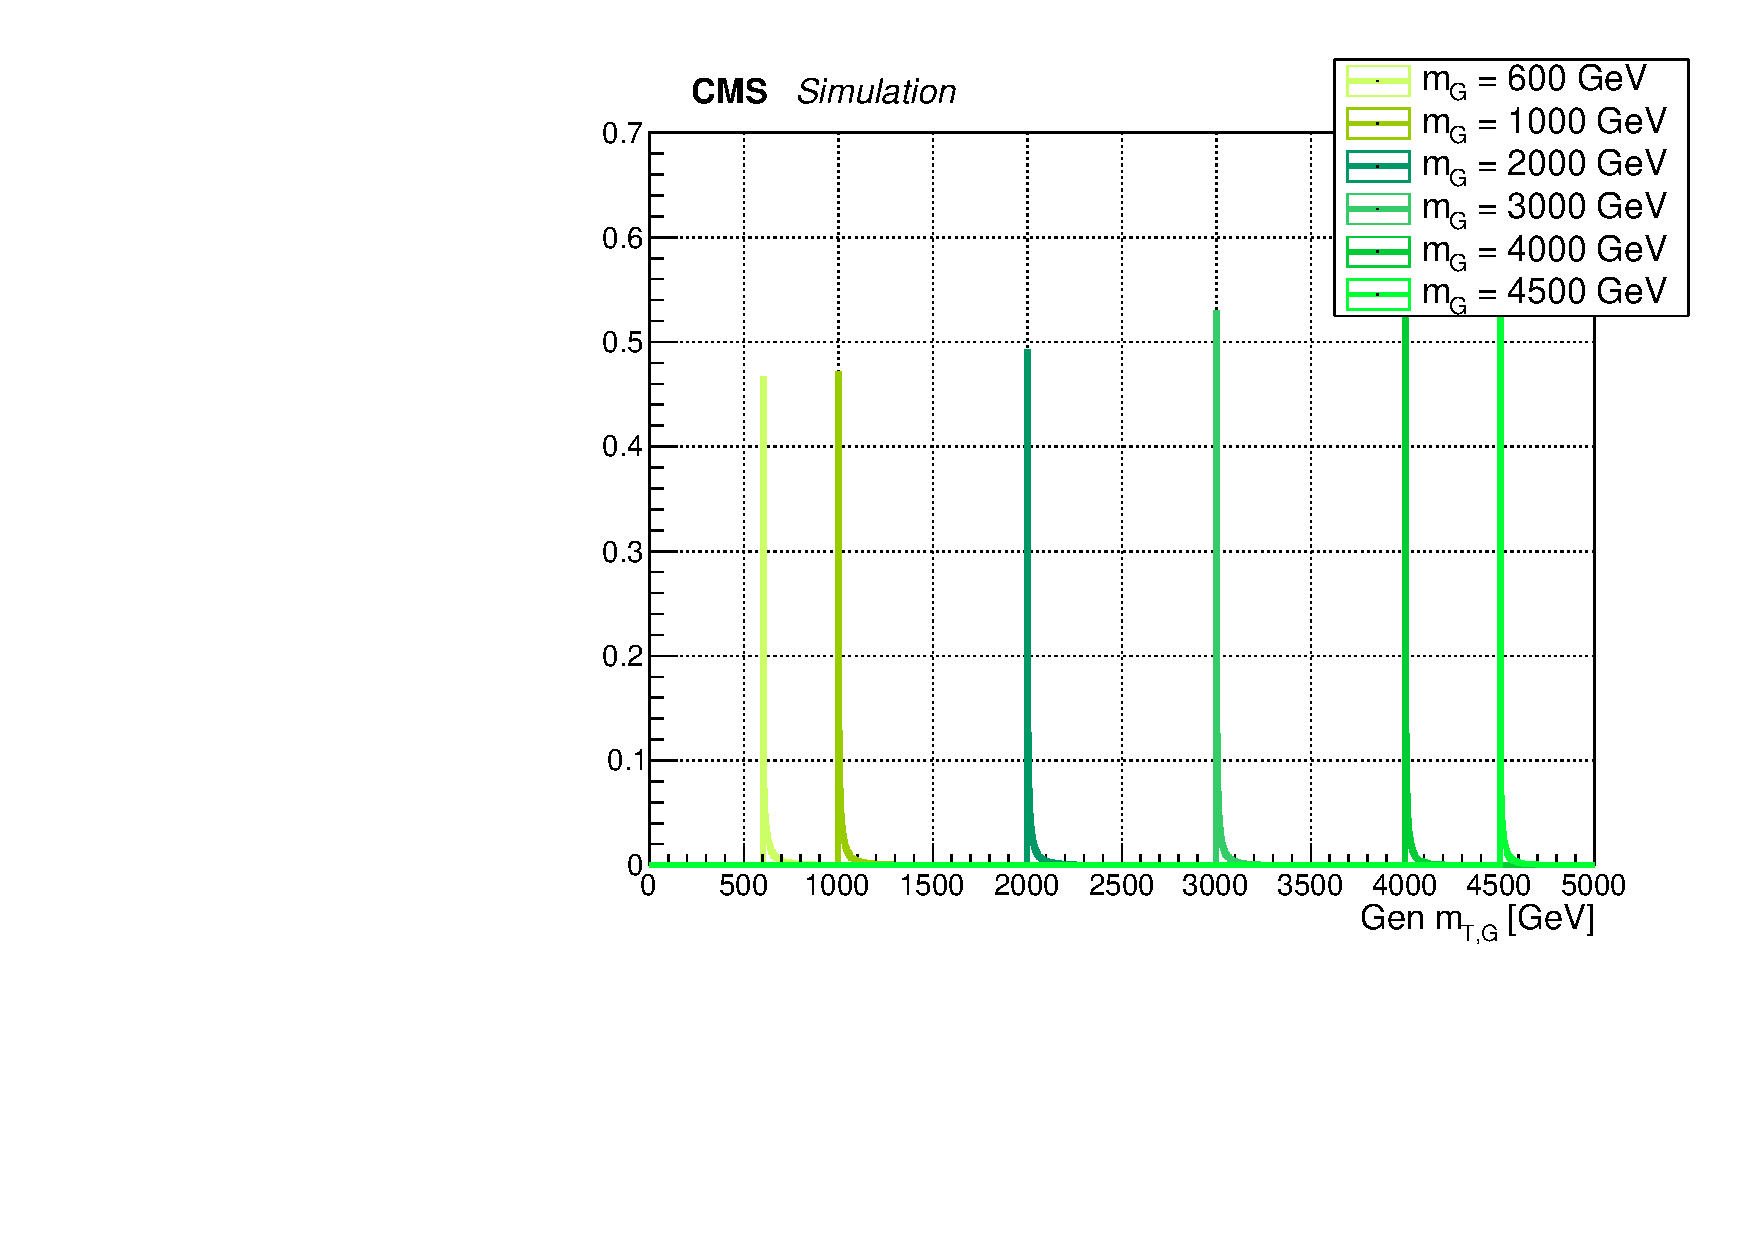
\includegraphics[width=.495\textwidth]{Gen_v9/XZZInv_g_XMT.pdf}%GenPhi1pt.pdf}
     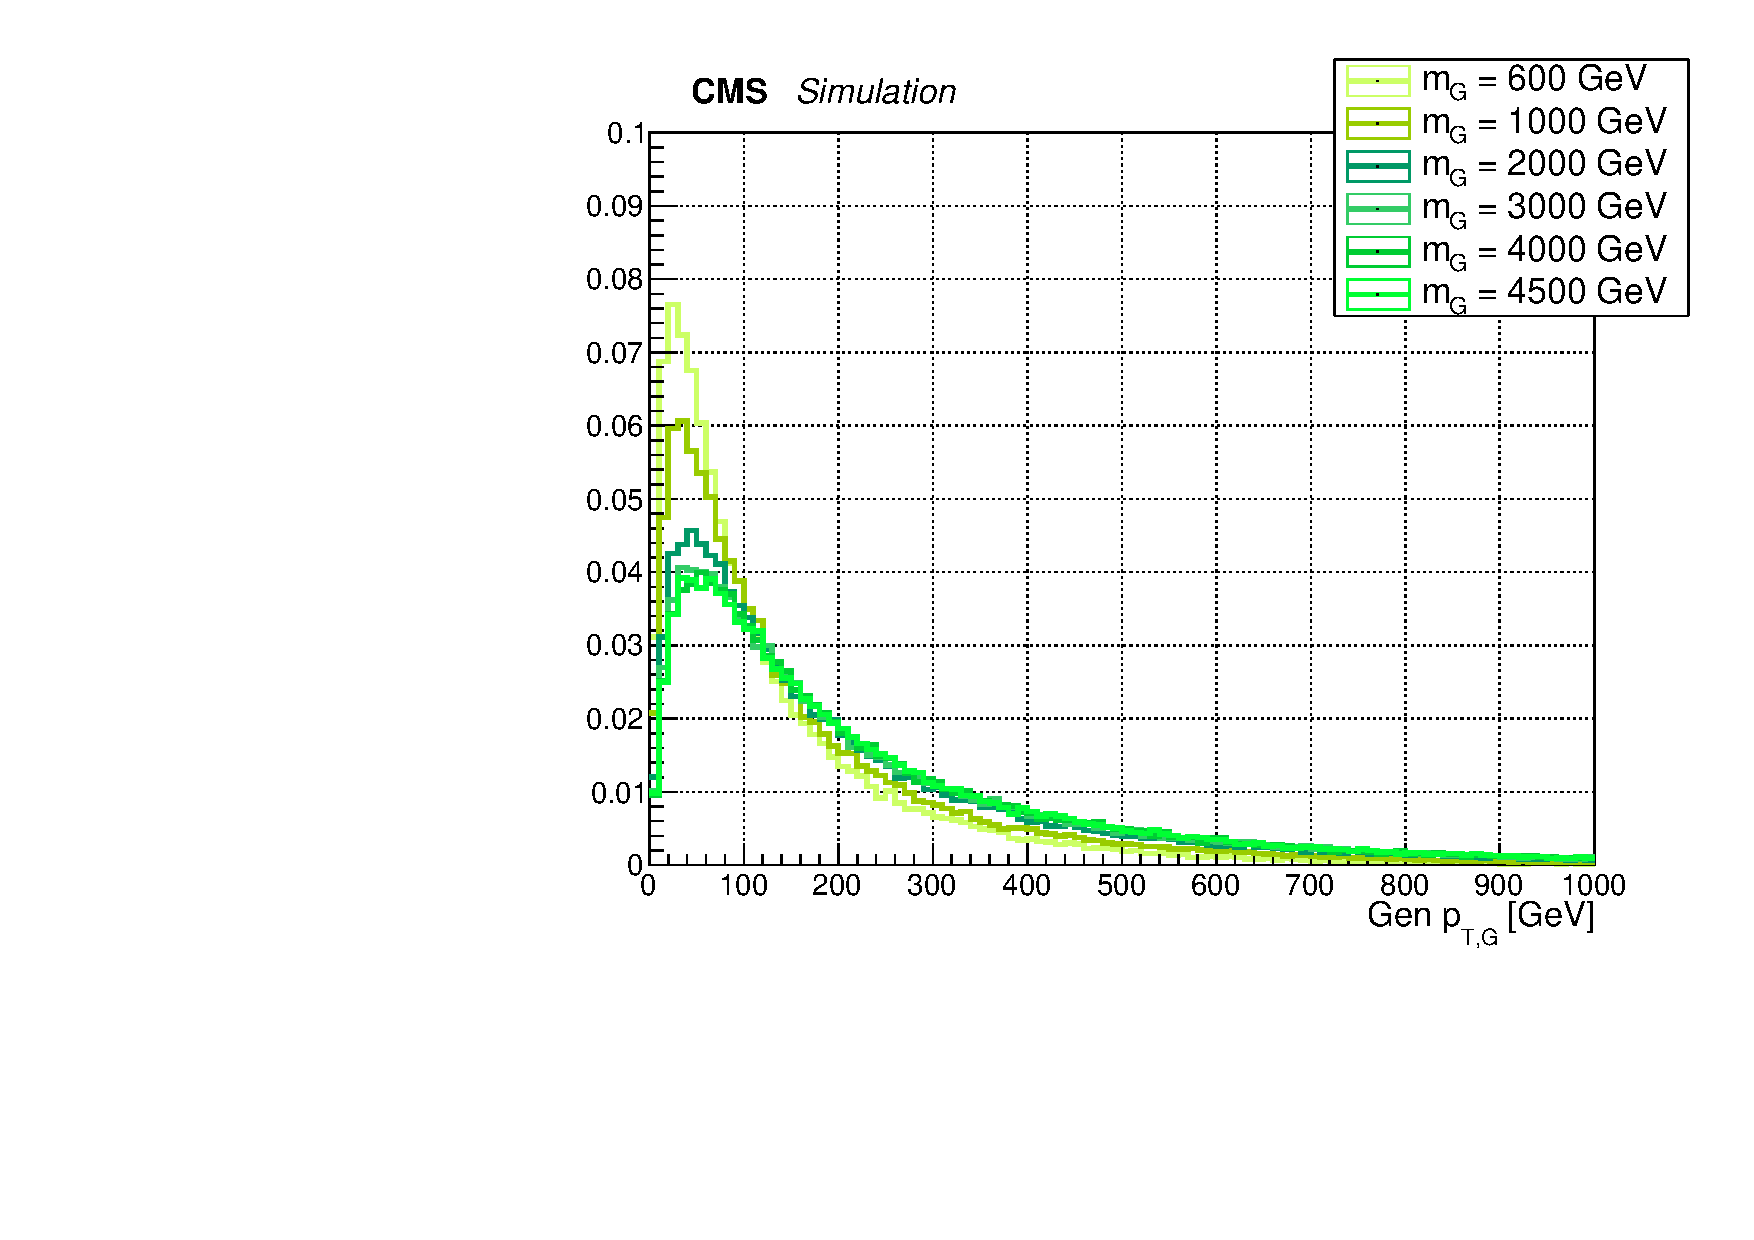
\includegraphics[width=.495\textwidth]{Gen_v9/XZZInv_g_XPt.pdf}%GenPhi1y.pdf}
     %\\
     %\includegraphics[width=.495\textwidth]{Gen_v7/g_ZLepMass.pdf}%GenZmass.pdf}
     %\includegraphics[width=.495\textwidth]{Gen_v7/g_ZHadMass.pdf}%GenHmass.pdf}
     \\
     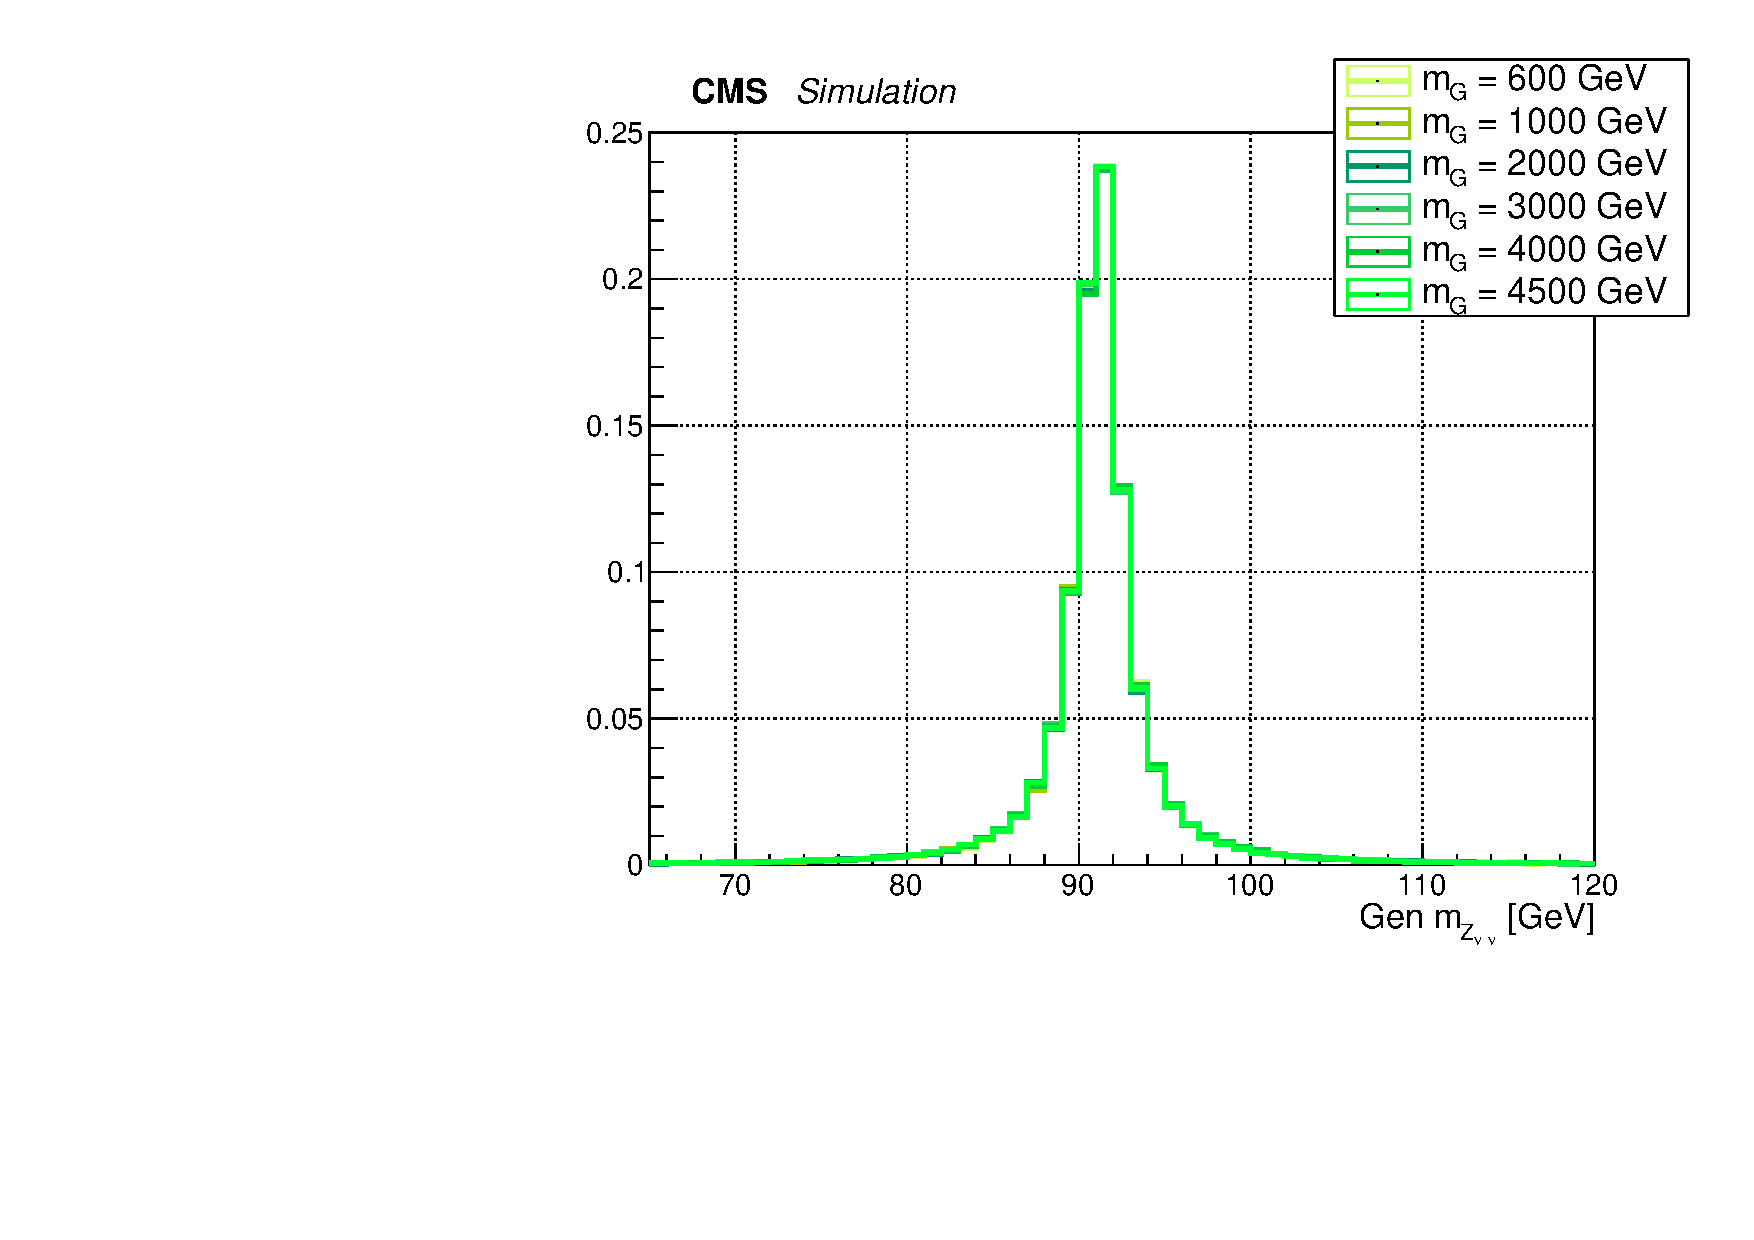
\includegraphics[width=.495\textwidth]{Gen_v9/XZZInv_g_ZLepMass.pdf}%GenZpt.pdf}
     \includegraphics[width=.495\textwidth]{Gen_v9/XZZInv_g_ZLepPt.pdf}%GenHpt.pdf}
     \\
     \includegraphics[width=.495\textwidth]{Gen_v9/XZZInv_g_VHadMass.pdf}%GenZdR.pdf}
     \includegraphics[width=.495\textwidth]{Gen_v9/XZZInv_g_VHadPt.pdf}%GenHdR.pdf}
   \end{center}
   \caption{Main signal kinematic quantities at generation level after parton showering, for spin-2 Bulk Graviton signal, considering different mass hypoteses ($m_{\G} = 0.6, 1, 2, 3, 4, 4.5$ TeV). Top: graviton transverse mass and \pt distributions. Center: invisibly decaying \Z mass and \pt. Bottom: hadronically decaying \Z mass and \pt.}
   \label{fig:genGravSignal1}
 \end{figure}

 \begin{figure}[!htb]
   \begin{center}
     \includegraphics[width=.495\textwidth]{Gen_v9/XZZInv_g_XRapidity.pdf}%GenPhi1pt.pdf}
     %\includegraphics[width=.495\textwidth]{Gen_v9/XZZInv_g_VZDR.pdf}%GenPhi1y.pdf}
     %\\
     %\includegraphics[width=.495\textwidth]{Gen_v7/g_ZLepMass.pdf}%GenZmass.pdf}
     %\includegraphics[width=.495\textwidth]{Gen_v7/g_ZHadMass.pdf}%GenHmass.pdf}
     \\
     \includegraphics[width=.495\textwidth]{Gen_v9/XZZInv_g_ZLepEta.pdf}%GenZpt.pdf}
     \includegraphics[width=.495\textwidth]{Gen_v9/XZZInv_g_Lep1Eta.pdf}%GenHpt.pdf}
     \\
     \includegraphics[width=.495\textwidth]{Gen_v9/XZZInv_g_VHadEta.pdf}%GenZdR.pdf}
     \includegraphics[width=.495\textwidth]{Gen_v9/XZZInv_g_Had1Eta.pdf}%GenHdR.pdf}
   \end{center}
   \caption{Main signal kinematic quantities at generation level after parton showering, for spin-2 Bulk Graviton signal, considering different mass hypoteses ($m_{\G} = 0.6, 1, 2, 3, 4, 4.5$ TeV). Top: graviton rapidity $\mathcal{Y}$. Center: pseudorapidity $\eta$ of the invisibly decaying \Z, and pseudorapidity of the leading neutrino. Bottom: pseudorapidity $\eta$ of the hadronically decaying \Z, and pseudorapidity of the leading quark.}
   \label{fig:genGravSignal2}
 \end{figure}

 \begin{figure}[!htb]
   \begin{center}
     \includegraphics[width=.495\textwidth]{Gen_v9/XZZInv_g_VZDPhi.pdf}%GenPhi1pt.pdf}
     \includegraphics[width=.495\textwidth]{Gen_v9/XZZInv_g_VZDR.pdf}%GenPhi1y.pdf}
     %\\
     %\includegraphics[width=.495\textwidth]{Gen_v7/g_ZLepMass.pdf}%GenZmass.pdf}
     %\includegraphics[width=.495\textwidth]{Gen_v7/g_ZHadMass.pdf}%GenHmass.pdf}
     \\
     \includegraphics[width=.495\textwidth]{Gen_v9/XZZInv_g_LepDR.pdf}%GenZpt.pdf}
     \includegraphics[width=.495\textwidth]{Gen_v9/XZZInv_g_HadDR.pdf}%GenHpt.pdf}
     \\
     \includegraphics[width=.495\textwidth]{Gen_v9/XZZInv_g_CosThetaStar.pdf}%GenZdR.pdf}
     \includegraphics[width=.495\textwidth]{Gen_v9/XZZInv_g_CosThetaJ.pdf}%GenHdR.pdf}
   \end{center}
   \caption{Main signal kinematic quantities at generation level after parton showering, for spin-2 Bulk Graviton signal, considering different mass hypoteses ($m_{\G} = 0.6, 1, 2, 3, 4, 4.5$ TeV). Top: angular separation in the transverse plane $\Delta \phi$ (left) and solid angle $\Delta R$ (right) between leptonic \Z and hadronic \Z. Center: solid angle between the neutrinos and the quarks. Bottom: distribution of $\cos{\theta}^{*}$ and $\cos{\theta}_{J}$ (described in text).}
   \label{fig:genGravSignal3}
 \end{figure}

 \begin{figure}[!htb]
   \begin{center}
     \includegraphics[width=.495\textwidth]{Gen_v9/XWZInv_g_XMT.pdf}%GenPhi1pt.pdf}
     \includegraphics[width=.495\textwidth]{Gen_v9/XWZInv_g_XPt.pdf}%GenPhi1y.pdf}
     %\\
     %\includegraphics[width=.495\textwidth]{Gen_v7/g_ZLepMass.pdf}%GenZmass.pdf}
     %\includegraphics[width=.495\textwidth]{Gen_v7/g_ZHadMass.pdf}%GenHmass.pdf}
     \\
     \includegraphics[width=.495\textwidth]{Gen_v9/XWZInv_g_ZLepMass.pdf}%GenZpt.pdf}
     \includegraphics[width=.495\textwidth]{Gen_v9/XWZInv_g_ZLepPt.pdf}%GenHpt.pdf}
     \\
     \includegraphics[width=.495\textwidth]{Gen_v9/XWZInv_g_VHadMass.pdf}%GenZdR.pdf}
     \includegraphics[width=.495\textwidth]{Gen_v9/XWZInv_g_VHadPt.pdf}%GenHdR.pdf}
   \end{center}
   \caption{Main signal kinematic quantities at generation level after parton showering, for spin-1 \Wp signal, considering different mass hypoteses ($m_{\Wp} = 0.6, 1, 2, 3, 4, 4.5$ TeV). Top: \Wp transverse mass and \pt distributions. Center: invisibly decaying \Z mass and \pt. Bottom: hadronically decaying \W mass and \pt.}
   \label{fig:genWprimeSignal1}
 \end{figure}

 \begin{figure}[!htb]
   \begin{center}
     \includegraphics[width=.495\textwidth]{Gen_v9/XWZInv_g_XRapidity.pdf}%GenPhi1pt.pdf}
     %\includegraphics[width=.495\textwidth]{Gen_v9/XZZInv_g_VZDR.pdf}%GenPhi1y.pdf}
     %\\
     %\includegraphics[width=.495\textwidth]{Gen_v7/g_ZLepMass.pdf}%GenZmass.pdf}
     %\includegraphics[width=.495\textwidth]{Gen_v7/g_ZHadMass.pdf}%GenHmass.pdf}
     \\
     \includegraphics[width=.495\textwidth]{Gen_v9/XWZInv_g_ZLepEta.pdf}%GenZpt.pdf}
     \includegraphics[width=.495\textwidth]{Gen_v9/XWZInv_g_Lep1Eta.pdf}%GenHpt.pdf}
     \\
     \includegraphics[width=.495\textwidth]{Gen_v9/XWZInv_g_VHadEta.pdf}%GenZdR.pdf}
     \includegraphics[width=.495\textwidth]{Gen_v9/XWZInv_g_Had1Eta.pdf}%GenHdR.pdf}
   \end{center}
   \caption{Main signal kinematic quantities at generation level after parton showering, for spin-1 \Wp signal, considering different mass hypoteses ($m_{\Wp} = 0.6, 1, 2, 3, 4, 4.5$ TeV). Top: \Wp rapidity $\mathcal{Y}$. Center: pseudorapidity $\eta$ of the invisibly decaying \Z, and pseudorapidity of the leading neutrino. Bottom: pseudorapidity $\eta$ of the hadronically decaying \W, and pseudorapidity of the leading quark.}
   \label{fig:genWprimeSignal2}
 \end{figure}

 \begin{figure}[!htb]
   \begin{center}
     \includegraphics[width=.495\textwidth]{Gen_v9/XWZInv_g_VZDPhi.pdf}%GenPhi1pt.pdf}
     \includegraphics[width=.495\textwidth]{Gen_v9/XWZInv_g_VZDR.pdf}%GenPhi1y.pdf}
     %\\
     %\includegraphics[width=.495\textwidth]{Gen_v7/g_ZLepMass.pdf}%GenZmass.pdf}
     %\includegraphics[width=.495\textwidth]{Gen_v7/g_ZHadMass.pdf}%GenHmass.pdf}
     \\
     \includegraphics[width=.495\textwidth]{Gen_v9/XWZInv_g_LepDR.pdf}%GenZpt.pdf}
     \includegraphics[width=.495\textwidth]{Gen_v9/XWZInv_g_HadDR.pdf}%GenHpt.pdf}
     \\
     \includegraphics[width=.495\textwidth]{Gen_v9/XWZInv_g_CosThetaStar.pdf}%GenZdR.pdf}
     \includegraphics[width=.495\textwidth]{Gen_v9/XWZInv_g_CosThetaJ.pdf}%GenHdR.pdf}
   \end{center}
   \caption{Main signal kinematic quantities at generation level after parton showering, for spin-1 \Wp signal, considering different mass hypoteses ($m_{\Wp} = 0.6, 1, 2, 3, 4, 4.5$ TeV). Top: angular separation in the transverse plane $\Delta \phi$ (left) and solid angle $\Delta R$ (right) between leptonic \Z and hadronic \W. Center: solid angle between the neutrinos and the quarks. Bottom: distribution of $\cos{\theta}^{*}$ and $\cos{\theta}_{J}$ (described in text).}
   \label{fig:genWprimeSignal3}
 \end{figure}

\clearpage

\noindent Angular distributions are related to the spin, the polarization and the kinematics of the produced resonance; in particular:
\begin{itemize}
\item the $\Delta R$ among neutrinos and quarks reflect the boosted nature of the electroweak bosons: the more massive the resonance, the larger the boost, and hence the closer the fermions. By looking at fig.~\ref{fig:genGravSignal3}-\ref{fig:genWprimeSignal3}, with a jet clustering parameter of 0.8 (AK8 jet) it is possible to enclose the quarks produced by the decay of the \V boson, for a resonance mass over 1 \TeV;
%\item the resonance rapidity $\mathcal{Y}$ is sensitive to the production mechanism
\item the $\cos{\theta}^{*}$, namely the cosine of the angle between the momentum of the \V boson, calculated in the resonance rest frame, and the flight direction of the resonance itself in the laboratory frame. This variable depends on the spin of the diboson resonance (spin-2 and spin-1 distributions are different, fig.~\ref{fig:genGravSignal3}-\ref{fig:genWprimeSignal3}). % This variable affects the p T distributions of bosons. When cos θ ∗ = 0, the p T of bosons in the lab frame, for a given X mass, reaches the maximum value and the new resonance X has a symmetric decay where the two bosons have equal p T ’s in the lab frame.
\item the $\cos{\theta}_J$, the cosine of the angle between the momentum of the leading quark, calculated in the \V rest frame, and the flight direction of the \V boson in the laboratory frame. This variable depends on the polarization state of the decay bosons~\cite{Khachatryan:2014vla}; in both HVT and bulk graviton model, electroweak bosons are expected to be longitudinally polarized. When $\cos{\theta}_J \rightarrow 0$, quarks are produced very close in angle and hence it is difficult to disentangle the two substructures in the large-cone jet (sec.~\ref{ssec:jetsub}); when $\cos{\theta}_J \rightarrow \pi$ the quarks are emitted asymmetrically (one is softer than the other).% asymmetric production -> tau21 can fail. This variable affects the pruned mass and the jet substructure variables (e.g. τ 21 ). The pruning algorithm and the τ 21 selections preferentially select jets that are split more symmetrically, which corresponds to a cos θ 1 value closer to zero.
\end{itemize}
 


\subsection{Background samples}\label{ssec:backgrounds}

The physics processes yielding final states with two neutrinos in association with a pair of quarks are considered as sources of background; they are listed in tab.~\ref{tab:bkg_datasets1}, along with the expected cross-sections at next-to-leading order (NLO) or next-to-next-to leading (NNLO).

\begin{itemize}
  \item {\bf Z + jets}: this process represents the main irreducible background for the signal. The production of a \Z boson in association with one or more partons in the final state has a similar topology to the signal. This \Z+jets background is produced in samples binned in \pt of the \Z boson starting from 100 \GeV with the {\sc aMC@NLO} generator, with FXFX merging~\cite{bib:FXFX}. The contribution from events with $\pt<100$~GeV is negligible after we require the \met to be greater than 200~\GeV (sec.~\ref{sec:selections}).

  \item {\bf W + jets}: the leptonic decay of a \W boson can be an irreducible background in the case the charged lepton escapes undetected (e.g. outside the detector acceptance) or fails the lepton identification requirements. The production of a \W boson has a cross section larger by an order of magnitude with respect to the \Z, and this makes the \W+jets a relevant background also when a lepton veto is applied. This \W+jets background is produced in samples binned in \pt of the \W boson starting from 100 \GeV with the {\sc aMC@NLO} generator.% \W+jets background binned in \HT (the sum of the \pt of the hadrons at generator level) starting from 100 \GeV with the \MADGRAPH LO generator are kept as backup samples.
\color{red}
  \item $\mathbf{top}$: production of \ttbar pairs represents a particularly challenging background at the LHC, given its large production cross section. These events always contain two energetic b-jets and two \W bosons which may decay to leptons that escape the detector or fail to be identified as leptons. Inclusive \ttbar decays have been considered. The primary handles to reduce the \ttbar background are topological, such as the azimuthal opening angle between the \Z boson and the dijet system, which is more broadly distributed in top pair production than in signal events. In \ttbar production the dilepton mass is not resonating in the Z mass region, and their \pt spectrum is sharply falling, given the absence of a single boosted resonance. This analysis makes use of \ttbar samples based on \POWHEG v2~\cite{bib:POWHEGst} NLO generator.
  Single-top and single-antitop samples are produced in the 5-flavours scheme using \POWHEG v2~\cite{bib:POWHEGtt} NLO generator.
  
  \item {\bf Diboson}: the production of two vector bosons in the SM is a rare process inducing and irreducible background for this search, with a similar kinematics to that of the signal. 
  Inclusive diboson production processes (\W\W, \W\Z, \Z\Z) are considered.
\end{itemize}




%\begin{sidewaystable}[!htb]\centering
\begin{table}[!htb]\centering
\caption{Simulated samples. The cross section $\times$ branching ratio is shown in \pb.\label{tab:bkg_datasets1} (*) cross sections taken from McM.}
\begin{tabular}{lcccc}
 Signal process &  Kinematical cuts & Generator & $\sigma\times\mathcal{B}$ [pb] & Events \\
 \hline 
$Z \rightarrow \nu \nu$ + jets & $100 < p_{T,Z} < 250$ \GeV & amcatnloFXFX -- Pythia8 &170.4 & 5353639\\
$Z \rightarrow \nu \nu$ + jets & $100 < p_{T,Z} < 250$ \GeV & amcatnloFXFX -- Pythia8 &170.4 & 5356674\\

$Z \rightarrow \nu \nu$ + jets & $250 < p_{T,Z} < 400$ \GeV & amcatnloFXFX -- Pythia8 & 6.636 & 1052985\\
$Z \rightarrow \nu \nu$ + jets & $250 < p_{T,Z} < 400$ \GeV & amcatnloFXFX -- Pythia8 & 6.636 & 1059634\\
$Z \rightarrow \nu \nu$ + jets & $400 < p_{T,Z} < 650$ \GeV & amcatnloFXFX -- Pythia8 & 0.9372 & 1050705\\
$Z \rightarrow \nu \nu$ + jets & $400 < p_{T,Z} < 650$ \GeV & amcatnloFXFX -- Pythia8 & 0.9372 & 1050592\\
$Z \rightarrow \nu \nu$ + jets & $p_{T,Z} > 650$ \GeV & amcatnloFXFX -- Pythia8 & 0.1042 & 1022595\\
$Z \rightarrow \nu \nu$ + jets & $p_{T,Z} > 650$ \GeV & amcatnloFXFX -- Pythia8 & 0.1042 & 1024620\\
\hline
$W \rightarrow \ell \nu$ + jets & $100 < p_{T,W} < 250$ \GeV & amcatnloFXFX -- Pythia8 & 676.3 & 10089661\\
$W \rightarrow \ell \nu$ + jets & $100 < p_{T,W} < 250$ \GeV & amcatnloFXFX -- Pythia8 & 676.3& 10088599\\
$W \rightarrow \ell \nu$ + jets & $250 < p_{T,W} < 400$ \GeV & amcatnloFXFX -- Pythia8 & 23.94 & 1001250\\
$W \rightarrow \ell \nu$ + jets & $250 < p_{T,W} < 400$ \GeV & amcatnloFXFX -- Pythia8 & 23.94 & 1000132\\
$W \rightarrow \ell \nu$ + jets & $400 < p_{T,W} < 650$ \GeV & amcatnloFXFX -- Pythia8 & 3.031 & 951713\\
$W \rightarrow \ell \nu$ + jets & $400 < p_{T,W} < 650$ \GeV & amcatnloFXFX -- Pythia8 & 3.031 & 988234\\
$W \rightarrow \ell \nu$ + jets & $p_{T,W} < 650$ \GeV & amcatnloFXFX -- Pythia8 & 0.4524 & 989482\\
$W \rightarrow \ell \nu$ + jets & $p_{T,W} > 650$ \GeV & amcatnloFXFX -- Pythia8 & 0.4524 & 985127\\
%%
%%
%WJetsToLNu\_HT-100To200\_TuneCUETP8M1\_13TeV-madgraphMLM-pythia8\_ext1-v1 & 1292.0 & 35244500 \\
%WJetsToLNu\_HT-200To400\_TuneCUETP8M1\_13TeV-madgraphMLM-pythia8\_ext1-v1 & 385.9 & 19851624 \\
%WJetsToLNu\_HT-400To600\_TuneCUETP8M1\_13TeV-madgraphMLM-pythia8-v1 & 47. & 7432746 \\
%WJetsToLNu\_HT-600To800\_TuneCUETP8M1\_13TeV-madgraphMLM-pythia8-v1 & 12.8 & 3722395\\
%WJetsToLNu\_HT-800To1200\_TuneCUETP8M1\_13TeV-madgraphMLM-pythia8-v2 & 5.261 & 1540477 \\
%WJetsToLNu\_HT-1200To2500\_TuneCUETP8M1\_13TeV-madgraphMLM-pythia8\_ext1-v1 & 1.334 & 7063909\\
%WJetsToLNu\_HT-2500ToInf\_TuneCUETP8M1\_13TeV-madgraphMLM-pythia8-v1 & 0.03089 & 2254248 \\
\hline
\ttbar inclusive & - & Powheg -- Pythia8 & 831.76 & 77229341 \\
$t$ ($tW$ channel) & - & Powheg -- Pythia8 & 35.85 & 6952830\\
5f inclusive \\
$\bar{t}$ ($\bar{t}W$ channel) & - & Powheg -- Pythia8 & 35.85 & 6933094\\
5f inclusive \\
$t$ (s-channel) & - & amcatnloFXFX -- Pythia8 & 3.344 & 622990\\
4f lepton decays \\
$t$ (t-channel) & - & Powheg -- Madspin -- Pythia8 & 136.02 & 67240808 \\
4f inclusive \\
$\bar{t}$ (t-channel) & - & Powheg -- Madspin -- Pythia8 & 80.95 & 38811017\\
4f inclusive \\
\hline
$WW$ inclusive & - & Pythia8 & $118.7$ & 994012\\%uncertianty: ^{+2.5\%}_{-2.2\%}
$WW$ inclusive & - & Pythia8 & 118.7 & 6987124\\
$WZ$ inclusive & - & Pythia8 & 47.2 & 1000000\\
$WZ$ inclusive & - & Pythia8 & 47.2 & 2995828\\
$ZZ$ inclusive & - & Pythia8 & 16.6 & 990064 \\
$ZZ$ inclusive & - & Pythia8 & 16.6 & 998034\\
\hline


\end{tabular}
%\end{sidewaystable}
\end{table}

\clearpage

\subsection{V boson momentum corrections}

%\subsubsection{NLO QCD}

%In Run II, the use of next-to-leading order generators, such as aMCatNLO, allowed to have a much better description of the vector bosons (\Z, \W) with respect to Run I, when only leading order generators were available. This is confirmed by data/simulation comparison. Unfortunately, NLO genarators have not been used to generate large exclusive samples with the high statistics needed for analyses in the high-\pt regime. Instead, exclusive \MADGRAPH samples are available. In these, the \pt spectra of the (\W and) \Z bosons is know to be non-perfecly described, compared to data and the inclusive aMCatNLO sample, as seen in Fig.~\ref{fig:kfactors1}-left. Corrections are derived to improve the simulation description. Instead of a correction function as a function of the \pt at generation level, separate multiplicative factors (k-factors) are derived for exclusive \MADGRAPH starting from the inclusive aMCatNLO smaple, in order to take into account the effect of QCD NLO processes.


%The Spring16 campaign has been produced using the same GEN fragments of the previous Spring15 samples.
%The analysis is therfore currently exploiting the k-factors evaluated in B2G-16-003~\cite{CMS:2016dzw} using Spring15 simulated samples.


%The procedure to derive the k-factors is the following. Since in the V \pt spectum there is overlap between the HT-binned exclusive samples, one solution could be to separate the \pt spectrum in at least four regions and solve a linear system for the normalization of the samples in each of these regions. However, the transverse momentum at generation level of a certain exclusive sample never goes above upper HT threshold. This is always true before showering, but even after taking showering into account the effect is very small ($<0.3\%$). The matrix representing the linear system can thus be considered diagonal, and a simpler approach is followed. The ratio between the inclusive and the higher-HT exclusive sample, normalized to the corresponding cross sections and eveluated in the \pt range above the lower HT threshold, is taken as the k-factor for the sample, and its normalization is then considered as fixed. In the following steps, k-factors for the lower HT exclusive sample are evaluated with the same procedure, but taking into account the fixed contribution of the exclusive samples with higher-HT binning.

%% This k-factor extraction procedure will be performed for DYJetsToLL samples. 
%% Small differences arise, but generally the k-factor can be as large as 1.5 in the lower part of the \pt spectrum, and very close to 1 in the higher-HT samples. 
%The numerical results obtained in B2G-16-003~\cite{CMS:2016dzw} are reported in Table~\ref{tab:kfactors}. 
%% The agreement with the inclusive NLO sample after the reweighting is flat at 1, and is reported in Figure~\ref{fig:kfactors1} and~\ref{fig:kfactors2}.

%\begin{figure}[!htb]
% \centering
%   \includegraphics[width=.495\textwidth]{figures/GenWJetsToLNuRatio.pdf}
%   %\includegraphics[width=.495\textwidth]{figures/GenDYJetsToLLRatio.pdf}
% \caption{\pt spectrum for the inclusive NLO and exclusive LO samples for the $\W \to \ell\nu$ process after the k-factor application, from B2G-16-003~\cite{CMS:2016dzw}.}
% \label{fig:kfactors1}
%\end{figure}

%% \begin{figure}[!htb]
%%  \centering
%%    \includegraphics[width=.495\textwidth]{figures/GenDYJetsToNuNuRatio.pdf}
%%    \includegraphics[width=.495\textwidth]{figures/GenWJetsToLNuRatio.pdf}
%%  \caption{\pt spectrum for the inclusive NLO and exclusive LO samples for the $\Z \to \nu\nu$ (\cmsLeft) and $\W \to\ell\nu$  processes (\cmsRight) after the k-factor application.}
%%  \label{fig:kfactors2}
%% \end{figure}
% 

%\begin{table}[!htb]\centering
%\begin{tabular}{lc}
% \hline
% Dataset & k-factor \\
%% \hline
%%DYJetsToLL\_M-50\_HT-100to200 & 1.588 \\
%%DYJetsToLL\_M-50\_HT-200to400 & 1.438 \\
%%DYJetsToLL\_M-50\_HT-400to600 & 1.494 \\
%%DYJetsToLL\_M-50\_HT-600toInf & 1.139 \\
%% \hline
%% ZJetsToNuNu\_HT-100To200 & 1.626 \\
%% ZJetsToNuNu\_HT-200To400 & 1.617 \\
%% ZJetsToNuNu\_HT-400To600 & 1.459 \\
%% ZJetsToNuNu\_HT-600ToInf & 1.391 \\
% \hline
% WJetsToLNu\_HT-100To200 & 1.459 \\
% WJetsToLNu\_HT-200To400 & 1.434 \\
% WJetsToLNu\_HT-400To600 & 1.532 \\
% WJetsToLNu\_HT-600ToInf & 1.004 \\
%\hline
%\end{tabular}
%\caption{K-factors for the V+jets samples.}
%\label{tab:kfactors}
%\end{table}


\subsubsection{NLO Electroweak}

Corrections to the V \pt spectrum comes from NLO electroweak contributions, that are enhanced at \TeV scale. These corrections are effectively applied on a per-event basis depending on the \pt of the vector boson at generation level. The calculation of these contributions is explained in Ref.~\cite{Kallweit:2015dum}. Figure~\ref{fig:ewk} shows the amount of the correction for the \W and \Z bosons.


\begin{figure}[!htb]
 \centering
   \includegraphics[width=.75\textwidth]{figures/EWK.pdf}
 \caption{Electroweak corrections for the \Z (green line) and \W boson (purple line) as a function of the transverse momentum~\cite{Kallweit:2015dum}.}
 \label{fig:ewk}
\end{figure}


%\clearpage

\subsection{Data}
\label{sec:data}

Data samples used in this analysis have been collected during 2016 RunB, RunC, RunD, RunE, RunF, RunG and RunH, at a center-of-mass energy of 13 TeV, in 25ns runs and with the magnetic field enabled. The {\tt MET} datasets are used for data selected with a \met trigger. {\tt SingleMuon} and {\tt SingleElectron} datasets are used to measure trigger efficiency on data. The full list of datasets used is shown in Table~\ref{tab:datasets}. Data is processed from {\tt ReMiniAOD} campaign.

The JSON file used in the analysis is the following:
\begin{itemize}
%   \item[{\bf Golden}:] {\tt Cert\_271036-275125\_13TeV\_PromptReco\_Collisions16\_JSON.txt} includes all the runs certified as ``good'' for all subsystems. The integrated luminosity amounts to $3.99$ \fbinv.
  \item[{\bf Golden}:] {\tt Cert\_271036-284044\_13TeV\_23Sep2016ReReco\_Collisions16\_JSON.txt} includes all the runs certified as ``good'' for all subsystems. The integrated luminosity amounts to $35.867$ \fbinv.
\end{itemize}


%\begin{figure}[!htb]
%  \begin{center}
%    \includegraphics[width=.495\textwidth]{figures/int_lumi_per_day_cumulative_pp_2016.pdf}
%  \end{center}
%  \caption{Cumulative luminosity versus day delivered to (blue), and recorded by CMS (orange) during stable beams and for pp collisions at 13 TeV centre-of-mass energy in 2016. The delivered luminosity accounts for the luminosity delivered from the start of stable beams until the LHC requests CMS to turn off the sensitive detectors to allow a beam dump or beam studies. Given is the luminosity as determined from counting rates measured by the luminosity detectors}
%  \label{fig:lumi}
%\end{figure}

% The ``golden'' JSON file is applied for categories that require a full PF event description, and make use of the PF missing energy; this is the case of the zero- and 1-lepton channels. In the 2-lepton channel, PF \MET is not used, and an list of runs and lumisections are included in the ``silver'' JSON file.

In order to remove problematic or noise-dominated events, the following list of filters~\cite{JMETPOG_filt}(ICHEP version) have been applied on data and MC:

\begin{itemize}
  \item {\tt HBHENoiseFilter}
  \item {\tt HBHENoiseIsoFilter}
  \item {\tt EcalDeadCellTriggerPrimitiveFilter}
  \item {\tt goodVertices}
  \item {\tt eeBadScFilter} (not recommended for Monte Carlo, hence not applied)
  \item {\tt globalTightHalo2016Filter}
    \item {\tt BadPFMuonFilter}
    \item {\tt BadChargedCandidateFilter}
\end{itemize}

\begin{table}[!htb]
\centering
  \caption{Datasets Run2016B-H.\label{tab:datasets}}
 \begin{tabular}{l} 
 \hline
 Dataset \\
 \hline
 MET/Run2016B-03Feb2017-v2 \\
 MET/Run2016C-03Feb2017-v1 \\
 MET/Run2016D-03Feb2017-v1 \\
 MET/Run2016E-03Feb2017-v1 \\
 MET/Run2016F-03Feb2017-v1 \\
 MET/Run2016G-03Feb2017-v1 \\
 MET/Run2016H-03Feb2017\_ver2-v1 \\
 MET/Run2016H-03Feb2017\_ver3-v1 \\
 \hline
 SingleMuon/Run2016B-03Feb2017-v2 \\
 SingleMuon/Run2016C-03Feb2017-v1 \\
 SingleMuon/Run2016D-03Feb2017-v1 \\
 SingleMuon/Run2016E-03Feb2017-v1 \\
 SingleMuon/Run2016F-03Feb2017-v1 \\
 SingleMuon/Run2016G-03Feb2017-v1 \\
 SingleMuon/Run2016H-03Feb2017\_ver1-v1 \\
 SingleMuon/Run2016H-03Feb2017\_ver2-v1 \\
 \hline
 SingleElectron/Run2016B-03Feb2017-v2 \\
 SingleElectron/Run2016C-03Feb2017-v1 \\
 SingleElectron/Run2016D-03Feb2017-v1 \\
 SingleElectron/Run2016E-03Feb2017-v1 \\
 SingleElectron/Run2016F-03Feb2017-v1 \\
 SingleElectron/Run2016G-03Feb2017-v1 \\
 SingleElectron/Run2016H-03Feb2017\_ver2-v1 \\
 SingleElectron/Run2016H-03Feb2017\_ver3-v1 \\
 \hline
 \end{tabular}
\end{table}

\clearpage

\subsection{Trigger}\label{ssec:trigger}

Events are selected on-line by a two-stage trigger. The Level 1 (L1) trigger consists of hardware processors that perform a very basic selection and counting of physics objects, and reduce the rate from 40 MHz down to 100 kHz. Events passing the L1 decision are acquired by the DAQ system, and a complete and more accurate reconstruction is performed by the High Level Trigger (HLT), which exploits similar but faster variations of the same algorithms used in the offline event reconstruction. A trigger path is a string that identifies a list of selections performed at HLT.
\met triggers have been used in this analysis: they are the logic OR of different trigger quantities, with thresholds on both the \met and the ${H}_T^{\text{miss}}$ computed using particle flow objects. 

The list of triggers used, along with the L1 seeds, is reported in Table~\ref{tab:trig_default}.

\begin{table}[!htb]
\centering
  \caption{HLT trigger paths used in the analysis.\label{tab:trig_default}}
 \begin{tabular}{l|r} 
 \hline
 HLT path & L1 seeds\\
% \hline
%\texttt{HLT\_Mu45\_2p1} \\
% \texttt{HLT\_TkMu50} \\
% \texttt{HLT\_Mu50} \\
% \hline       
%\texttt{HLT\_Ele105\_CaloIdVT\_GsfTrkIdT} \\
%\texttt{HLT\_Ele115\_CaloIdVT\_GsfTrkIdT} \\
 \hline
 \hline
 \texttt{HLT\_PFMETNoMu90\_PFMHTNoMu90\_IDTight} & \texttt{L1\_ETM70 OR} \\
& \texttt{L1\_DoubleJetC56\_ETM60 OR}\\
&  \texttt{L1\_ETM60 OR L1\_ETM50}\\
 \hline
 \texttt{HLT\_PFMETNoMu110\_PFMHTNoMu110\_IDTight} & \texttt{L1\_ETM70 OR} \\
& \texttt{L1\_DoubleJetC56\_ETM60 OR}\\
&  \texttt{L1\_ETM60 OR L1\_ETM50}\\
 \hline
 \texttt{HLT\_PFMETNoMu120\_PFMHTNoMu120\_IDTight} & \texttt{L1\_ETM70 OR} \\
& \texttt{L1\_DoubleJetC56\_ETM60 OR}\\
&  \texttt{L1\_ETM60 OR L1\_ETM50}\\
\hline
 \texttt{HLT\_PFMET170\_NoiseCleaned or} & \texttt{L1\_ETM60 OR L1\_ETM70}\\
\hline
 \texttt{HLT\_PFMET170\_JetIdCleaned or} & \texttt{L1\_ETM60 OR L1\_ETM70}\\
\hline
 \texttt{HLT\_PFMET170\_HBHECleaned} & \texttt{L1\_ETM60 OR L1\_ETM70}\\
 \hline
 \end{tabular}
\end{table}

%On principle, the same set of trigger paths should be re required to be fired for both data and simulated events.
%However, in the current version of the MiniAOD samples the trigger information is not present (or not valid for the HLT paths included). %Therefore the trigger is not required to have fired in MC.
The approach adopted in this analysis consists in calculating the trigger efficiency on data, and applying the measured efficiency to Monte Carlo samples. Therefore the trigger is not required to have fired in MC.

The efficiency of the \met triggers is measured on {\tt SingleMuon} dataset by selecting $\W \to \mu \nu$ events using a single muon trigger ({\tt HLT\_IsoMu24 OR HLT\_IsoTkMu24\_v}), asking to have one isolated {\tt TightId} muon, with the suitable \pt threshold to be in the plateu of the muon trigger. The efficiency has been calculated as a function of the minimum quantity between the offline reconstructed missing transverse momentum, where the contribution of the muon is subtracted from the \met computation as in the online algorithm, and the offline ${H}_T^{\text{miss}}$, defined as ${H}_T^{\text{miss}} = \sum_{j}^{\text{n. of AK4 jets}} p_T^{j}$. This approach guarantees to mimic the behaviour of the online L1 trigger seeds. The detailed selections:
\begin{itemize}
\item {\tt HLT\_IsoMu24\_v OR HLT\_IsoTkMu24\_v}
\item 1 muon, tight ID, \pt$>35$ GeV, tight isolation
\item at least one AK8 jet, \pt$>170$ GeV, $|\eta<|2.5$, LooseID
\item AK4 jets included in ${H}_T^{\text{miss}}$: \pt$>30$ GeV, $|\eta<|2.5$, LooseID
\end{itemize}

The efficiency of the \met triggers has independently been measured also on {\tt SingleElectron} dataset, by selecting $\W \rightarrow e \nu$ events using a single electron trigger ({\tt HLT\_Ele27\_WPLoose\_Gsf OR HLT\_Ele27\_WPTight\_GsfOR HLT\_Ele32\_WPTight\_Gsf}), asking to have one {\tt TightId} electron, with the suitable \pt threshold, and asking to the electron and the \met to be separated in $\phi$ in order to suppress fake events ($\Delta \phi > 0.5$).
\begin{itemize}
\item {\tt HLT\_Ele27\_WPLoose\_Gsf OR HLT\_Ele27\_WPTight\_GsfOR HLT\_Ele32\_WPTight\_Gsf}
\item 1 electron, tight ID, \pt$>35$ GeV
\item at least one AK8 jet, \pt$>170$ GeV, $|\eta<|2.5$, LooseID
\item AK4 jets included in ${H}_T^{\text{miss}}$: \pt$>30$ GeV, $|\eta<|2.5$, LooseID
\end{itemize}


%The contributions of passed-failed events coming from both datasets have been added together.
The full available statistics has been employed to derive the efficiency. The final turn-on curve for the \met trigger used in this analysis is shown in fig.\ref{fig:MetTrigMu}-\ref{fig:MetTrigEle}, divided in muon-electron dataset. The {\tt METNoMu} trigger efficiencies are displayed separately, together with their OR. The quantity plotted in the x axis depends on the dataset, according to what was explained previously.

The difference needed to cover the gap between these two curves is taken as trigger systematic uncertainty, and it amounts to 1\% at 200 GeV. %A complete description of the method used to derive trigger efficencies and scale factor can be found in Ref. [25]. Trigger scale factors are applied consistently in simulation to take into account residual efficiency differences.
%[SISTEMA LA REFERENZA]

%The efficiencies of the single muon triggers are provided centrally by the Muon POG~\cite{MuonSF} with a tag and probe procedure by selecting $\Z \to \ell\ell$ events.
%HighPt lepton ID and tracker isolation requirements are applied to the \emph{probes}. The trigger efficiency is then evaluated studying the \emph{tag} lepton efficiency as a function of both \pt and $\eta$ for both data and MC.
%The muon trigger efficiency is applied consistently to the simulation throughout the analysis.
%The average scale factor for the triggers used is about $\--\%$.

%Figure~\ref{fig:MuonTrig} shows the trigger efficiency as centrally provided by the muon POG.

 \begin{figure}[!htb]
   \begin{center}
     \includegraphics[width=.7\textwidth]{Efficiency/ZhadZinv/TriggerTurnOn_SingleMuAllRunsmin_met_mht_nomu_Lmu3.pdf}
   \end{center}
   \caption{\met trigger efficiency for the \met trigger paths used in this analysis, calculated on {\tt SingleMuon} dataset.}
   \label{fig:MetTrigMu}
 \end{figure}

 \begin{figure}[!htb]
   \begin{center}
     \includegraphics[width=.7\textwidth]{Efficiency/ZhadZinv/TriggerTurnOn_SingleEleAllRunsmin_met_mhtele3.pdf}
   \end{center}
   \caption{\met trigger efficiency for the \met trigger paths used in this analysis, calculated on {\tt SingleElectron} dataset.}
   \label{fig:MetTrigEle}
 \end{figure}

\clearpage



%\section{Event selection}
\label{sec:objects}

In this section, a list of the physics objects used in the analysis is presented, together with performance and validation plots. 

The objects are selected according to the standard Run2 reccomendations provided by the various POGs for the Summer16 (25ns) MiniAOD-v2 (Moriond reccomendations).

The version of CMSSW used for the analysis is {\tt CMSSW\_8\_0\_25}.

\subsection{Vertex and Pile-up}
{\color{red} How the vertices and pile-up are reconstructed}

Due to pileup several primary vertices are typically reconstructed in an event.
The primary vertex of the event is defined as the one with the highest sum of transverse momenta $\sum \pt^2$ of clustered physics objects associated to it, which passes the following selections:
\begin{itemize}
  \item number of degrees of freedom $N_{DoF}>4$
  \item vertex position along the beampipe $|z_{vtx}|<24\cm$
  \item vertex distance with respect the beam pipe $d_0<2\cm$
\end{itemize}
where $z_{vtx}$ and $d_0$ are the distance along and perpendicular to the beam line of the vertex with respect the nominal interaction point $(0,0,0)$.

The data sample contains a significant number of additional interactions per bunch crossing, an effect known as pileup (PU). 

The {\tt Summer16} \texttt{v2} MINIAOD Monte Carlo samples are generated simulating the PU conditions, using the 25ns asymptotic PU scenario. 
Nevertheless, the MC PU description does not match exactly the conditions in data, and there is therefore the need to reweight the simulated events in order to improve the agreement with the data. 

The MC samples are reweighted using the standard CMS PU reweighting technique~\cite{bib:pureweight,bib:pureweight2} assuming a total inelastic cross section of $\sigma_{in} = 69\,200 \mu b$.

The comparison between the distributions of primary vertices in data and MC after the PU reweighting is applied is shown in Figure~\ref{fig:npv} for an event selection (called inclusive selection) requiring large amount of \met recoiling against an AK8 fat jet~(Tab.~\ref{tab:sel}).
 
 \begin{figure}[!htb]
  \centering
    %\includegraphics[width=.495\textwidth]{plots/v9_U/XVZnnInc/nPV.pdf}
  \caption{Primary vertices distributions after reweighting with the official recipe and $\sigma_{in}=69\,200 \mu b$.}
  \label{fig:npv}
 \end{figure}


\subsection{Electrons}\label{ssec:electrons}
{\color{red} How the electrons are reconstructed}

Electrons are reconstructed from energy deposits in the ECAL matched to tracks reconstructed in the silicon tracker. 
The electron trajectories are reconstructed using a dedicated modeling of the electron energy loss and fitted with a Gaussian sum filter.
Electrons used in this analysis are required to pass the Particle Flow criteria, and to fall in the ECAL pseudorapidity fiducial range ($|\eta|<2.5$). 

The electron identification used in this analysis is based on the ``cut-based'' Id defined by the EGamma POG for the \texttt{Summer16} 25ns~\cite{EGammaPOG_ele}, and suggested also for the usage in 80X for the so-called Moriond dataset.
Isolation cuts are already applied within the cut-based Id definitions, therefore no additional Isolation cut is required.
In the isolation definition the effect of PU is considered by taking into account the energy deposits in the calorimeter, estimated through the so-called \emph{$\rho$-area} method, by subtracting the median energy density in the event $\rho$ multiplied by electron effective area.
The isolation value is computed in a $\Delta$R cone of 0.3 centered along the lepton direction.

Since in this analysis we are aiming at a final state without any lepton, every electron identified with \emph{veto} cut-based Id, transverse momentum $\pt > 10$ GeV is vetoed. The detailed set of cuts to define a \emph{veto} cut-based Id electron are reported in the Table~\ref{tab:EGcutBar}.

%The detailed set of cuts are reported in the Table~\ref{tab:EGcutBar}. $\Delta \eta_{in}^{seed}$ and $\Delta \varphi_{in}$ are the difference in $\eta$ and $\varphi$ between the track position as measured in the inner layer, extrapolated to the interaction vertex and then extrapolated to the calorimeter and the $\eta$ of the seed cluster or the $\varphi$ of the supercluster, $H/E$ is the ratio of the hadronic energy of the CaloTowers in a cone of radius 0.15 centred on the electron's position in the calorimeter to the electromagnetic energy of the electron's supercluster, $\sigma_{i\eta i\eta}$ is the spread in eta in units of crystals of the electrons energy in 5x5 block centred on the seed crystal, and $1/E - 1/p$ is the difference of the inverse of the energy and the momentum.
% $E^{2x5}/E^{5x5}$ is fraction of energy in 2x5 crystals around seed to the energy in 5x5 crystals around the seed, 

\begin{table}[htb]
 \centering
    \begin{tabular}{lccc}
     \hline

    Electrons                   &        & \multicolumn{2}{c}{\texttt{Veto}}\\
                                &        & EB      & EE     \\
 \hline
    $\sigma_{i\eta i\eta} $     & $ < $  &0.0115   &0.037  \\
    $\Delta \eta_{in}^{seed}$   & $ < $  &0.00749  &0.00895 \\
    $\Delta \varphi_{in} $      & $ < $  &0.228    &0.213   \\
    $H/E $                      & $ < $  &0.356    &0.211   \\
    relIso (EA)                 & $<$    &0.175    &0.159   \\
    $|1/E - 1/p|$               & $ < $  &0.299    &0.15    \\
    $|d_0|$                     & $ < $  &0.05     &0.10   \\
    $|d_z|$                     & $ < $  &0.10     &0.20   \\
    missing hits                & $\leq$ &2        &3       \\
    conversion veto             &        &  yes    &yes     \\
    
 \hline
\end{tabular}
\caption{ Summer16 cut-based selection for 25ns conditions. EB: barrel cuts ( $|\eta_\text{supercluster}| \leq 1.479$); EE: endcap cuts ( $|\eta_\text{supercluster}| > 1.479$)}
\label{tab:EGcutBar}
\end{table}

Scale factors for electron identification (including isolation) are provided by Egamma POG, derived for 80X (Moriond 17 recommendation), that can be found in~\cite{EGammaPOG_ele_SF}.


%\clearpage

\subsection{Muons}\label{ssec:muons}

{\color{red} How the muons are reconstructed}

In the standard CMS reconstruction for $pp$ collisions, muon tracks are first reconstructed independently in the inner tracker (tracker track) and in the muon system (standalone-muon track). Based on these objects, two reconstruction approaches are used~\cite{bib:CMS-PAPER-MUO-10-004}: \emph{Global Muon} (outside-in) and \emph{Tracker Muon} (inside-out).
\begin{itemize}
  \item[\emph{Global Muon reconstruction (outside-in)}:] for each standalone-muon track, a matching tracker track is found by comparing parameters of the two tracks propagated onto a common surface, and a global-muon track is fitted combining hits from the tracker track and standalone-muon track, using the Kalman-filter technique~\cite{bib:kalman}. At large transverse momenta, $\pt > 200 \GeV$, the global-muon fit can improve the momentum resolution compared to the tracker-only fit.
  \item[\emph{Tracker Muon reconstruction (inside-out)}:] in this approach, all tracker tracks with $\pt > 0.5 \GeV$ and the total momentum $p > 2.5 \GeV$ are considered as possible muon candidates and are extrapolated to the muon system taking into account the magnetic field, the average expected energy losses, and multiple scattering in the detector material. If at least one muon segment (i.e., a short track stub made of DT or CSC hits) matches the extrapolated track, the corresponding tracker track qualifies as a Tracker Muon.
\end{itemize}

Tracker Muon reconstruction is more efficient than the Global Muon reconstruction at low momenta, $\pt \lesssim 5 \GeV$, because it requires only a single muon segment in the muon system, whereas Global Muon reconstruction is designed to have high efficiency for muons penetrating through more than one muon station and typically requires segments in at least two muon stations. Thanks to the high tracker-track efficiency and a very high efficiency of reconstructing segments in the muon system, about 99\% of muons produced in $pp$ collisions and having sufficiently high momentum are reconstructed either as a Global Muon or a Tracker Muon, and very often as both. Muons reconstructed only as standalone-muon tracks have worse momentum resolution and less favorable collision muon to cosmic-ray muon ratio than the Global and Tracker Muons and are usually not used in physics analyses.

Muons are usually based on the \emph{Particle Flow Muon} selection, considering Global Muon or a Tracker Muon candidates and by applying minimal requirements on the track components in the muon system and taking into account a matching with small energy deposits in the calorimeters. %However, in the boosted $\Z \to \mu\mu$ regimes, muons have similar problems to electrons. The Global muon reconstruction suffers a drop in efficiency as the $\Delta R$ between the muon decreases. This is a consequence of the seeding algorithm, which includes in the seed some segments of the other muon, and after the final muon trajectory builder, a cleaning is applied based on the number of segments and the $\chi^2$ of the muon track. After the cleaning, only one muon track is selected among the group of tracks that share segments, and this effect avoids the reconstruction of the other muon (Figure~\ref{fig:Muon_Multi}).

%The reconstruction of muons very close in $\Delta R$ is also a problem for the PF algorithm, which is based on the hypothesis that the muon is a minimum-ionizing particle. Another high-\pt track close to a reconstructed muon can also fail to pass the PF identification of the nearby muon, further lowering the efficiency at small angles, as shown in Figure~\ref{fig:Muon_Multi}.
%The adopted compromise between efficiency and fake-muons rejection is then to require that \emph{at least} one of the two muons (not necessarily the highest-\pt) fulfills both the PF and the \texttt{HighPt}, while the other has to satisfy a looser selection. This asymmetric selections ensures a high efficiency ($\gtrsim 95\%$) in the whole \pt, $\eta$ %(Figure~\ref{fig:Muon_pt_eta})
%and $\Delta R$ ranges (Figure~\ref{fig:Muon_Multi}). 
%The \texttt{HighPt} Id is a set of cuts specifically designed for high-momentum muons from the Muon POG~\cite{MuonPOG}:

%\begin{itemize}
%   \item to be reconstructed also as Global muon
%   \item at least one muon chamber hit included in the global-muon track fit
%   \item muon segments in at least two muon stations
%   \item the track used to obtain the muon momentum needs to pass $\delta\pt/\pt < 0.3$
%   \item tracker track transverse impact parameter $d_{xy} < \unit{2}{\text{mm}}$ w.r.t. the primary vertex
%   \item longitudinal impact parameter $d_z < \unit{5}{\text{mm}}$ w.r.t. the primary vertex
%   \item number of pixel hits $>0$
%   \item number of tracker layers with hits $> 5$.
%\end{itemize}

%The other muons in the event, if present, should be identified with a tracker-only selection. A tight \texttt{CustomTracker} Id is defined using the same quality cuts on the muon track as the \texttt{HighPt}, but dropping the requirements that force the muon to be Global or PF:

%\begin{itemize}
%    \item to be reconstructed as a standard Tracker muon (was Global muon in HightPt Id)
%    \item at least one muon chamber hit included in the global-muon track fit
%    \item muon segments in at least two muon stations
%    \item the track used to obtain the muon momentum needs to pass $d\pt/\pt < 0.3$.
%    \item TuneP-track transverse impact parameter $d_{xy} < \unit{2}{\text{mm}}$ w.r.t. the primary vertex (was Tracker-track)
%    \item longitudinal impact parameter $d_z < \unit{5}{\text{mm}}$ w.r.t. the primary vertex
%    \item number of pixel hits $>0$
%    \item number of tracker layers with hits $> 5$.
%\end{itemize}

%Having dropped the PF identification requirements, the best estimation of the muon momentum is then extracted via the TuneP algorithm, better suited for high-\pt muons.

For muons reconstructed using the PF algorithm, the standard muon isolation is defined as the ratio of the \pt sum of all charged and neutral particle-flow candidates in the event within a cone with a radius of $\Delta R=0.4$ centered along the lepton direction. Corrections in order to reduce the PU contamination are also applied, using the $\Delta \beta$ method.
Charged candidates falling into the cone that are not compatible with the primary vertex are removed from the sum. Additionally, the neutral contribution from PU is estimated to be half the one coming from charged candidates, and this quantity is also subtracted from the total. Eventually, the scalar sum is divided by the lepton \pt itself. The general formula for the standard \emph{particle-flow} isolation is then:
$$I_{rel} = \left[ \sum \pt^\text{ch \ had} + \max(\sum \pt^\text{neu \ had} + \sum \pt^{\gamma} - 0.5 \cdot \sum \pt^\text{pu \ ch \ had}, \ 0) \right] /\pt^\ell $$
where $\sum \pt^\text{ch \ had}$ is the sum of the transverse momenta of the charged hadrons, $\sum \pt^\text{neu \ had}$ is the sum of transverse energies of the neutral hadrons, $\pt^{\gamma}$ is the sum of the transverse energy of particle flow photons and $\sum \pt^\text{pu \ ch \ had}$ is the sum of transverse momenta of the charged particles in the cone of interest but with particles not originating from the primary vertex (for pileup corrections). %With this definition of the isolation the other electron of the system does not enter the calculation.

%In the case of muons not reconstructed using the PF algorithm, as in the case of the \texttt{CustomTracker} id used to select muons in this analysis, the MuonPOG provides a Tracker-based definition of isolation.
%This isolation is computed as the scalar sum of the \pt of all the track from the leading PV in the event within a cone with a radius of $\Delta R=0.3$ centered along the muon direction, normalized by the muon \pt.

In the VZ event selection, all muons identified with the \texttt{Loose} standard id, \pt over 10 GeV, PF isolation below 0.25, $\eta<|2.4|$ are vetoed.

%In the VZ event selection, at least one muon is required to be identified with the \texttt{HighPt} standard id, while the other is selected if passes wither the \texttt{CustomTracker} requirements or the standard \texttt{HighPt}. The \emph{loose} working point ($<0.1$) of the tracker-based isolation criterion is used to select the leptons. When evaluating the tracker-isolation for each muon, if the other selected muon falls in the $\Delta R < 0.3$ isolation cone, the tracker-based isolation is recomputed after removing the inner tracker track \pt of the other muon.
 
Scale factors for muon identification and isolation are centrally provided as a function of the muon \pt and $\eta$ by the Muon POG~\cite{MuonSF}, and are applied consistently in the analysis.


\subsection{Taus}\label{sec:tau}
{\color{red} How the taus are reconstructed}
 
The presence of hadronically-decaying taus only act as veto for the events both in the signal and in the control regions to suppress electroweak backgrounds. The selection criteria for taus are $\pt > 18$ GeV and $|\eta| < 2.3$. The Run2 TauPOG recomended identification criteria~\cite{TauPOG} (\texttt{decayModeFinding}, \texttt{byLooseCombinedIsolationDeltaBetaCorr3Hits})  are required and applied in order to identify possible tau candidates.
% % The tau-lepton multiplicity in the inclusive $\Z \to \mu\mu$ is reported in Fig.~\ref{fig:ZmmInc_taupho}.
% 
\subsection{Photons}
{\color{red} How the photons are reconstructed}

As in the case of tau leptons, a photon veto is applied in the analysis both for the signal and the control regions.
Events are rejected if they contains one (or more) photon with $\pt > 15$ GeV , $|\eta| < 2.5$, passing the \texttt{Loose} cut-based photon ID. The \texttt{Loose} photon Id is applied as in the EGamma POG recommandations for Run2 analyses~\cite{EGammaPOG_pho} (tuned on \texttt{ Spring16} 25 ns samples).
The isolation cuts (using the rho-area method for the mitigation of the pileup) and conversion safe electron veto are applied.
The isolation value is computed in a $\Delta R$ cone of 0.3 and is corrected for pileup by subtracting the event-by-event energy density ($\rho$) times an effective area.
The applied cut-based definition of the \texttt{Loose} photon Id is reported in Table~\ref{tab:PhotonId}.
% % The photon multiplicity in the inclusive $\Z \to \mu\mu$ is reported in Fig.~\ref{fig:ZmmInc_taupho}.
% 
 \begin{table}[htb]
  \centering
     \begin{tabular}{lccc}
      \hline
 
     Photons                                   &       & \multicolumn{2}{c}{\texttt{Loose}}\\
                                               &       & EB      & EE  \\
  \hline
     $H/E $                                    & $ < $ &0.0597   & 0.0481      \\
     $\sigma_{i\eta i\eta} $                   & $ < $ &0.01031  & 0.03013   \\
     PF ch.had.iso.($\rho$-corr)               & $ < $ &1.295    & 1.011   \\
     PF neu.had.iso.($\rho$-corr)              & $ < $ &$10.910+0.0148\pt+0.000017\pt^2$    &$5.931+0.0163\pt+0.000014\pt^2 $   \\
     PF photon iso.($\rho$-corr)               & $ < $ &$3.630+0.0047\pt$                 &$6.641+0.0034\pt $   \\
     conversion veto                           &       & yes     &yes     \\
  \hline
 \end{tabular}
  \caption{Photon cut-based Id for Spring16 25ns conditions. EB: barrel cuts ( $|\eta_\text{supercluster}| \leq 1.479$); EE: endcap cuts ( $|\eta_\text{supercluster}| > 1.479$)}\label{tab:PhotonId}
 \end{table}

Scale factors for photon identification (including isolation) are provided by Egamma POG, derived for 80X (Moriond 17 recommendation), that can be found in~\cite{EGammaPOG_ele_SF}.

\clearpage


\subsection{Jets}\label{ssec:jets}
{\color{red} How the jets are reconstructed}

Events in the CMS detector are reconstructed using the particle-flow algorithm~\cite{bib:PF1,bib:PF2}, which combines information from all sub-detectors in order to reconstruct stable particles (muons, electrons, photons, neutral and charged hadrons). The charged hadron subtraction algorithm (CHS) removes candidates not associated to the primary vertex in order to remove contributions from pileup~\cite{CMS-PAS-JME-14-001}. The remaining particles are used as input to jet clustering algorithms to reconstruct particle-flow jets. The jets are clustered using the {\sc FastJet} package~\cite{bib:fastjet} with the anti-\kt jet clustering algorithm~\cite{Cacciari:2008gp} with a clustering parameter of $R = 0.8$ (``fat''-jets or AK8 jets) or $R = 0.4$ (``standard''-jets or AK4 jets). In order to avoid double-counting of PF candidates, AK4 jets are considered only if the angular separation from the leading AK8 jet is larger than $\Delta R>0.8$.
Several levels of jet energy corrections are applied to the momentum of the clustered (raw) jets in order to obtain the energy value that is closer to the true energy of the initial parton~\cite{bib:1748-0221-6-11-P11002}:

\begin{itemize}
  \item[\emph{L1 Offset}:] the pileup and electronic noise effects are removed. This correction can be estimated using events collected by a random trigger, without any preconditions except a beam crossing, referred as \emph{zero bias} events. The offset contribution from pileup is estimated by the FastJet method which relies on the definition of a jet area~\cite{bib:fastjet} from which a median energy density ($\rho$, in \GeV/Area) per event can be defined. The correction subtracted to the jet \pt equals to $\rho$ times the jet area. FastJet has the advantage of being able to remove the out-of-time pileup component, but has the disadvantage of subtracting the underlying event contribution as well.
  \item[\emph{L2 Relative ($\eta$)}:] the variation in jet response with $\eta$ is flattened. The unbalance between the jets transverse momentum that is observed on average, is due to the variation of the jet response across the detector versus $\eta$.
  \item[\emph{L3 Absolute (\pt)}:] the calorimetric energy response varies as a function of the jet \pt. The absolute correction removes these variations and makes the response equal to unity. This correction is obtained from simulation using the Monte Carlo truth information.
  \item[\emph{L2L3 Residual}:] differences between data and simulation after L2 and L3 corrections are removed by applying a specific calibration to data events. Residual corrections are extracted from data using the transverse momentum balance in $\gamma$+jets and \Z+jets events~\cite{bib:1748-0221-6-11-P11002}.
\end{itemize}

The latest jet energy corrections are applied to AK4 and AK8 CHS jets, and the tags are {\tt Summer16 23Sep2016V3}.

In this analysis, jets are considered if the corrected \pt is larger than 30 \GeV for AK4 jets and 200\GeV for AK8 jets, and lie in the tracker acceptance ($|\eta|<2.4$). Additionally, AK4 are required to pass \emph{loose} jet identification requirements, AK8 are required to pass \emph{tight} jet identification requirements defined by the JETMET POG for Run2 analyses~\cite{JetMETPOG}, listed in Table~\ref{tab:JetId}. AK8 jets are used to reconstruct the hadronically decaying electroweak boson candidate, whilst AK4 jets are used to suppress the contribution of top and QCD background events.

Figure~\ref{fig:n_AK8}-~\ref{fig:AK8jet_eta} show the data/simulation comparison after the analysis selections~(Tab.~\ref{tab:sel} without Top cleaning and Event cleaning).

\begin{table}[htb]
 \centering
 \begin{tabular}{lll}
\hline
PF Jet ID                       & \emph{loose}   & \emph{tight}   \\
\hline
Neutral Hadron Fraction         & $< 0.99  $     & $< 0.90  $    \\
Neutral EM Fraction             & $< 0.99  $     & $< 0.90  $\\
Number of Constituents          & $> 1     $     & $> 1     $\\
Muon Fraction                   & \--            & \-- \\
\hline
\multicolumn{3}{l}{Additionally, for $|\eta| < 2.4$ } \\
\hline
Charged Hadron Fraction         & $> 0   $& $> 0   $\\
Charged Multiplicity            & $> 0   $& $> 0   $\\
Charged EM Fraction             & $< 0.99$& $< 0.99$\\
\hline
 \end{tabular}
 \caption{ \emph{Loose} and \emph{Tight} jet identification requirements for Run2 (Spring16) 25ns conditions.\label{tab:JetId}}
\end{table}

\begin{figure}[!htb]
  \begin{center}
    %\includegraphics[width=.495\textwidth]{plots/v9_U/XVZnnInc/nFatJets.pdf}
  \end{center}
  \caption{Number of reconstructed AK8 jets after selections.}
  \label{fig:n_AK8}
\end{figure}

\begin{figure}[!htb]
  \begin{center}
    %\includegraphics[width=.495\textwidth]{plots/v9_U/XVZnnInc/FatJet1_pt.pdf}
  \end{center}
  \caption{Leading AK8 jet \pt spectra after selections.}
  \label{fig:AK8jet_pt}
\end{figure}

\begin{figure}[!htb]
  \begin{center}
    %\includegraphics[width=.495\textwidth]{plots/v9_U/XVZnnInc/FatJet1_eta.pdf}
  \end{center}
  \caption{Leading AK8 jet $\eta$ spectra after selections.}
  \label{fig:AK8jet_eta}
\end{figure}


Since it has been measured that the jet energy resolution (JER) is not the same in data and MC, an additional smearing is applied in simulation, in order to get a better agreement, as suggested by JETMET POG~\cite{bib:jetsmear}.

There are two independent ways to get the smearing. With the scaling method, corrected four-momentum of a reconstructed jet is rescaled with a factor
$$c_{\text{JER}} = 1 + (s_{\text{JER}} - 1) \frac{p_T - p_T^{\text{ptcl}}}{p_T},$$
where $p_T$ is its transverse momentum, $p_T^{\text{ptcl}}$ is the transverse momentum of the corresponding jet clustered from generator-level particles, and $s_{\text{JER}}$ is the data-to-simulation core resolution scale factor. Factor $c_{\text{JER}}$ is truncated at zero, i.e. if it is negative, it is set to zero.
This method only works if a well-matched particle-level jet is present and can result in a large shift of the response otherwise. The following requirements are imposed for the matching:
$$\Delta R < R_{\text{cone}} / 2, |p_T - p_T^{\text{ptcl}}| < 3 \sigma_{\text{JER}} p_{T}.$$
Here $R_{\text{cone}}$ is the jet cone size parameter (for instance, 0.4 for AK4 jets) and $\sigma_{\text{JER}}$ is the relative \pt resolution as measured in simulation.

An alternative approach, which does not require the presence of a matching particle-level jet, is the stochastic smearing. In this case corrected jet four-momentum is rescaled with a factor $$c_{\text{JER}} = 1 + \mathcal{N}(0, \sigma_{\text{JER}}) \sqrt{max(s_{\text{JER}}^2 - 1, 0)},$$ where $\sigma_{\text{JER}}$ and $s_{\text{JER}}$ are the relative \pt resolution in simulation and data-to-simulation scale factors, and $\mathcal{N}(0, \sigma)$ denotes a random number sampled from a normal distribution with a zero mean and variance $\sigma^2$. As before, scaling factor $c_{\text{JER}}$ is truncated at zero. This method only allows to degrade the resolution.

The smearing procedure adopted in this analysis is the hybrid method: when matching particle-level jet is found, the scaling method is used; otherwise the stochastic smearing is applied. The smearing coefficients and their errors, provided by JETMET POG, are reported in Tab.~\ref{tab:smear} for 2016 data (tag: {\tt Spring1625nsV10}).

\begin{table}[!htb]
  \centering
  \begin{tabular}{l|ccccccc}
    Jet $\eta$ & SF \\
    \hline
    $0.0-0.5$ & $1.109 \pm 0.008$ \\
    $0.5-0.8$ & $1.138 \pm 0.013$ \\
    $0.8-1.1$ & $1.114 \pm 0.013$ \\
    $1.1-1.3$ & $1.123 \pm 0.024$ \\
    $1.3-1.7$ & $1.084 \pm 0.011$ \\
    $1.7-1.9$ & $1.084 \pm 0.011$ \\
    $1.9-2.1$ & $1.140 \pm 0.047$ \\
    $2.1-2.3$ & $1.067 \pm 0.053$ \\
    $2.3-2.5$ & $1.177 \pm 0.041$ \\
    $2.5-2.8$ & $1.364 \pm 0.039$ \\
    $2.8-3.0$ & $1.857 \pm 0.071$ \\
    $3.0-3.2$ & $1.328 \pm 0.022$ \\
    $3.2-5.0$ & $1.16  \pm 0.029$ \\
  \end{tabular}
  
  \caption{Smearing coefficients and JER uncertainties.}
  \label{tab:smear}
\end{table}

\clearpage
\subsection{Jet mass}\label{ssec:jetmass}

The jet mass is the main observable in distinguishing a V-jet from a QCD jet. Jet grooming consists in the suppression of uncorrelated UE/PU (underlying event and pile-up) radiation from the target jet and improves the discrimination pushing the jet mass for QCD jets towards lower values while maintaining the jet mass for V-jets around the boson-mass.

%Two different grooming algorithms were originally considered:
The grooming algorithm considered in this analysis is the following:
\begin{itemize}
%%  \item[\bf{Trimming}:] Trimming is a technique that ignores regions within a jet that falls below a minimum \pt threshold. Trimming reclusters the jet's constituents with a radius $R_{sub}$ and then accepts only the subjets that have $p_{T,sub} > f_{cut}$, where $f_{cut}$ is typically taken proportional to \HT , the scalar sum of the \pt of all jet reconstructed in the event.
%%  \item[\bf{Filtering}:] This procedure provides a hierarchical structure for the clustering like the \kt algorithm, but in angles rather than in relative transverse momenta. It creates a series of n new subjects $s_1, s_2, \dots s_n$ ordered in descending \pt. The final jet is redefined as the sum of the four-momenta of the three highest \pt subjets $\sum_i^{min(n,3)} s_i$.
%  \item[\bf{Pruning}:] The idea is to take a jet of interest and then to recluster it using a vetoed sequential clustering algorithm. Clustering is performed with the CA algorithm, but particles are discarded if they are too far away in $\Delta R$: 
% %\begin{linenomath}\begin{equation}
% $$ \Delta R_{ij} > D_{cut} \alpha \frac{m_j}{p_{T,j}}$$
% %\end{equation}\end{linenomath}
%  and the energy sharing is too asymmetric: 
% % \begin{linenomath}\begin{equation}
% $$ z_{ij} = \frac{min(p_{T,i}, p_{T,j})}{p_{T,i+j}} < z_{cut} $$
% % \end{equation}\end{linenomath}
%  where $z_{cut}$ and $\alpha$ are parameters of the algorithm. If both these conditions are satisfied the softer of the two particles is not considered.
  \item[\bf{Soft-drop}:] The ``soft drop declustering'' is a jet substructure technique which recursively removes soft wide-angle radiation from a jet~\cite{Larkoski:2014wba}. The soft drop algorithm depends on two parameters: a soft threshold $z$ cut and an angular exponent $\beta$. Like any grooming method, soft drop declustering removes wide-angle soft radiation from a jet in order to mitigate the effects of contamination from initial state radiation (ISR), underlying event (UE), and multiple hadron scattering (pileup). Given a jet of radius $R_0$ with only two constituents, the soft drop procedure removes the softer constituent unless:
%\begin{linenomath}\begin{equation}
 $$\frac{\min(\pt^1,\pt^2)}{\pt^1+\pt^2} > z_{cut} \left( \frac{\Delta R_{12}}{R_0} \right)^\beta$$
%\end{equation}\end{linenomath}
By construction, this condition fail for wide-angle soft radiation. The degree of jet grooming is controlled by $z_{cut}$ and $\beta$, with $\beta \to \infty$ returning back an ungroomed jet.  The $\beta=0$ limit of the energy loss is particularly interesting, since it is largely insensitive to the value of the strong coupling constant. The default parameters used by CMS are $\beta=0$ and $z_{cut}=0.1$.
\end{itemize}

%In general, the filtering algorithm is the least aggressive grooming technique, with groomed jet masses close to the original case. The trimming algorithm is moderately aggressive and produces a much wider final mass distribution. Pruning is the most aggressive technique and a bimodal distribution begins to appear: in cases where the pruned jet mass is small, jets usually have most of their energy configured in core components with little gluon radiation, which leads to narrow jets. Instead, when the pruned jet mass is large, the jets are split more symmetrically.

The grooming algorithm, {\bf soft-drop}, is used in association with {\bf PUPPI} in order to remove soft and wide-angle radiations and the pile-up contribution. It is a shared choice among all the diboson analyses, praised by theoreticians.

Unfortunately, the default soft-drop + PUPPI jet mass suffers from a systematic shift from the expected value of about $\sim 10\%$, and some residual dependence on the jet \pt. Further corrections to the jet mass have been applied:

\begin{enumerate}
  \item[{\bf Gen}:] a \pt-dependent correction to account for a small shift in the generated vector boson mass, applied only on simulated samples
  \item[{\bf Reco}:] a \pt-dependent correction to the reconstructed jet mass, applied separately for jets in the barrel and endcaps regions
\end{enumerate}

These corrections are evaluated centrally by JMAR and documented in~\cite{AN-16-215}, and applied accordingly within the analysis.

Figure~\ref{fig:fatjet_pre_softdroppuppimass_ZZ}-~\ref{fig:fatjet_softdroppuppimass} show the jet mass for \PW or \Z bosons before and after the correction, without applying any cut on this variable.

\begin{figure}[!htb]
  \begin{center}
    %\includegraphics[width=.495\textwidth]{plots/v9/XVZnnPre/FatJet1_softdropPuppiMass_signalZZ.pdf}
    %\includegraphics[width=.495\textwidth]{plots/v9/XVZnnPre/FatJet1_softdropPuppiMassCorr_signalZZ.pdf}
  \end{center}
  \caption{Softdrop + PUPPI mass of AK8 jet reconstructed for different bulk graviton signal samples; left: before corrections. right: after corrections.}
  \label{fig:fatjet_pre_softdroppuppimass_ZZ}
\end{figure}

\begin{figure}[!htb]
  \begin{center}
    %\includegraphics[width=.495\textwidth]{plots/v9/XVZnnPre/FatJet1_softdropPuppiMass_signalWZ.pdf}
    %\includegraphics[width=.495\textwidth]{plots/v9/XVZnnPre/FatJet1_softdropPuppiMassCorr_signalWZ.pdf}
  \end{center}
  \caption{Softdrop + PUPPI mass of AK8 jet reconstructed for different $W^{'}$ signal samples; left: before corrections. right: after corrections.}
  \label{fig:fatjet_pre_softdroppuppimass_ZZ}
\end{figure}

\begin{figure}[!htb]
  \begin{center}
    %\includegraphics[width=.495\textwidth]{plots/v9/XVZnnPre/FatJet1_softdropPuppiMass.pdf}
    %\includegraphics[width=.495\textwidth]{plots/v9/XVZnnPre/FatJet1_softdropPuppiMassCorr.pdf}
  \end{center}
  \caption{Softdrop + PUPPI mass of AK8 jet; left: before corrections. right: after corrections.}
  \label{fig:fatjet_softdroppuppimass}
\end{figure}

Furthermore, in order to obtain a better data-Monte Carlo agreement, a smearing procedure has been applied to the puppi softdrop mass, by using the stochastic method, with a constant smearing coefficent provided by JETMET POG ($1.00 \pm 0.20$), that does not depend on jet pseudorapidity if it is restricted to $|\eta|<2.5$.

%\clearpage
\subsection{Jet substructure}\label{ssec:jetsub}

In order to further discriminate signal from background, it useful to investigate the inner structure of the jet. Studying the distribution of the jet constituents with respect to the jet axis allows us to test the hypothesis of the existence of multiple substructures, that could be evidence of jets originated by more than one parton. This procedure proceeds as follows: the constituents of the jet are clustered again with the $k_T$ algorithm, however the procedure is stopped when one obtains N subjets. 
Then, a new variable, the N-subjectiness, is introduced. It is defined as:
%\begin{linenomath}\begin{equation}
$$\tau_N = \frac{1}{d_0} \sum_k p_{T,k} min( \Delta R_{1,k}^\beta, \Delta R_{2,k}^\beta, \dots, \Delta R_{N,k}^\beta )$$
%\end{equation}\end{linenomath}
where $\beta$ is an arbitrary parameter, the index $k$ runs over the jet constituents and the distances $\Delta R_{N,k}$ are calculated with respect to the axis of the N-th subjet, obtained by one iteration of $\tau$ minimization by varying the subjet axes around the $k_T$ subjet axes.

The normalization factor $d_0$ is calculated as $d_0 = \sum_k p_{T, k} R_0^\beta$, setting $R_0$ to the radius of the original jet.
The N-subjettiness is always included in the interval from 0 to 1 and represents the compatibility of the jet structure with an N-subjet hypothesis: small values correspond to high compatibility. Indeed, $\tau_N$ weights the transverse momentum of the jet constituents by their angular distance to the closest subjet.
In this analysis the N-subjettiness is calculated from the ungroomed jet with the parameter $\beta=1$. The subjettiness related to the one and two subjet hypothesis is thus:
%\begin{linenomath}\begin{equation}
$$\tau_1 = \frac{1}{d_0} \sum_k p_{T,k} \Delta R_{1,k}$$
%\end{equation}\end{linenomath}
and
%\begin{linenomath}\begin{equation}
$$\tau_2 = \frac{1}{d_0} \sum_k p_{T,k} min( \Delta R_{1,k}, \Delta R_{2,k} )$$
%\end{equation}\end{linenomath}
In principle, these two quantities should allow us to distinguish the dipole-like
nature of the showering of the Higgs decay from the classic monopole structure of
QCD jets. In particular, the variable that best discriminates between V-jets and
QCD jets is the ratio of 2-subjettiness and 1-subjettiness, $\tau_{21} = \tau_2 / \tau_1$.

Figure~\ref{fig:fatjet_pre_tau21} shows the $\tau_{21}$ distributions for the PUPPI algorithm.

\begin{figure}[!htb]
  \begin{center}
    %\includegraphics[width=.495\textwidth]{plots/v9_U/XVZnnInc/FatJet1_puppiTau21.pdf}
  \end{center}
  \caption{$\tau_{21}$ subjettiness of PUPPI AK8 jet after inclusive selections.}
  \label{fig:fatjet_pre_tau21}
\end{figure}



\subsection{b-tagging}\label{ssec:btagging}
 
%The presence of a pair of b-quarks from the $\htobb$ decay is a very distinctive signature that permits a strong discrimination against all the backgrounds that involve jets with light flavors. The only  background which cannot be reduced with this technique is the $\Z$ production in association with one or two b-quarks, and the $\Z \to \bbbar$ decay which is also topologically similar to the signal. The latter can be only reduced by applying a jet mass cut, as described in Section~\ref{ssec:jetmass}.
% 
%Tagging b-jets in boosted topologies has been undergone several modifications with respect to Run-I taggers. 
% One of the most important differences is that the tagger algorithms are not directly based on tracks. 
%%Run-II b-taggers are by default applied on the same charged particle-flow candidate list that is used in the jet clustering (\emph{explicit jet-to-track association}). This procedure is applied to subjets as well: b-tagging algorithms are applied to both the fat-jet and the sub-jets, independently. Furthermore, thanks to the explicit jet-to-track association, the two sub-jets do not share any PF-constituent, avoiding unintended correlations.
B-tagging algorithms are applied to both the fat-jet and the sub-jets, independently. For subjets, run-II taggers are by default applied on the same charged particle-flow candidate list that is used in the jet clustering (\emph{explicit jet-to-track association}). Thanks to the explicit jet-to-track association, the two sub-jets do not share any PF-constituent, avoiding unintended correlations.
% 
% 
%Several algorithms have been developed to tag jets from b-quarks. The recommended and best-performing algorithm is the {\tt pfCombinedInclusiveSecondaryVertexV2BJetTags}, often shortened to \emph{combined secondary vertex (CSV)}. This algorithm involves the use of secondary vertices, together with other lifetime information, like the IP significance or decay lengths. Secondary vertices are reconstructed with the inclusive vertex finder algorithm, that does not require jets (and thus is independent on the jet size) and uses all tracks to reconstruct secondary vertices~\cite{cms:JHEP032011136}. %In order to provide discrimination even when no secondary vertices are found, so the maximum possible b-tagging efficiency is not limited by the secondary vertex reconstruction efficiency ($50 \sim 60\%$). In many cases, tracks with an IP significance $> 2$ can be combined in a so-called pseudo vertex, allowing for the computation of a subset of secondary vertex based quantities even without an actual vertex fit. When even this is not possible, a no vertex category reverts simply to track based variables similarly to the jet probability algorithm. %The list of variables fed as input to an Artificial Neural Network is:
% \begin{itemize}
%   \item  the vertex category (real, pseudo, or no vertex)
%   \item  2D flight distance significance
%   \item  vertex mass
%   \item  number of tracks at the vertex
%   \item  ratio of the energy carried by tracks at the vertex with respect to all tracks in the jet
%   \item  the pseudo-rapidity of the tracks at the vertex with respect to the jet axis
%   \item  2D IP significance of the first track that raises the invariant mass above the charm threshold of 1.5 \GeV when subsequently summing up tracks ordered by decreasing IP significance
%   \item  3D signed IP significances for all tracks in the jet
%   \item  number of tracks in the jet
%   \item  $\Delta R$ between the secondary vertex flight direction and the jet axis
%   \item  number of secondary vertices associated to the jet or sub-jet
% \end{itemize}
 
The jet or sub-jet is considered as tagged if the discriminator value is above some threshold value, often referred to as the cut value, and the efficiency is defined as the number of jets which have a discriminator value that is above that cut divided by the total number of jets (of the same flavor).
% %In other words, the integral of the histogram from a certain discriminator cut up to infinity divided by the total number of jets.
%The typical b-tagging efficiency is between 40\% and 70\% while keeping the rate of mis-identified light-flavor jets between 0.1\% and 10\%. Three working points are usually defined for each algorithm, defining cuts in the discriminators based on the level of mis-tagging. The cut values and the corresponding mis-tagging for light-flavor jets relative to the CSV algorithm are reported in Table~\ref{tab:csvwp}.
% 
% \begin{table}[!htb]
%   \begin{center}
%   \begin{tabular}{lcc}
%   Working point & Cut & $\varepsilon_{light}$\\
%   \hline
%    Loose & 0.605  & $\sim 10\%$ \\
%    Medium & 0.890  & $\sim 1\%$ \\
%    Tight & 0.970  & $\sim 0.1\%$ \\
%   \end{tabular}
%   \end{center}
%   \caption{CSV official working points.}
%   \label{tab:csvwp}
% \end{table}

The b-tagging algorithm used to set the analysis strategy is the Combined Secondary Vertex (CSV)~\cite{bib:btag} discriminator (full name {\tt pfCombinedInclusiveSecondaryVertexV2BJetTags}). Different working points are provided by the POG for Run2 analyses~\cite{BTVPOG}, as shown in table~\ref{tab:btag}, but the only one used in this analysis is the \emph{loose} working point.

\begin{table}[!htb]
  \centering
  \label{tab:btag}
  \begin{tabular}{l|c|c}
     Working point & CSV cut & mis-tag probability\\ 
    \hline
     CSVL (Loose)  & $>0.5426$ & $\approx 10\%$  \\ 
     CSVM (Medium) & $>0.8484$ & $\approx 1\%$   \\ 
     CSVT (Tight)  & $>0.9535$ & $\approx 0.1\%$ \\ 
    \hline
  \end{tabular}
  \caption{Working point for CSV b-tagging algorithm.}
  
\end{table}

B-tagging efficiency is not the same in data and MC. In order to take into account this difference, the BTV POG provides collections of b-tagging scale factors for b-jets and mistagged light jets, measured for different physics processes, for the supported tagging algorithms and the three standard working points~\cite{bib:btag}. A weight is calculated on a per-event basis as a function of the b-tagging status of the jets and their kinematic variables~\cite{bib:btagsf}.%; this is a simple and effective method if there are a small number of possible combinations of jets and b-tagged jets.%Unfortunately, this is not the case of the present analysis. Other techniques allow to take into account the scale factors provided by BTV by \emph{reshaping} the discriminator output; this method has been already successfully applied in the SM VH analysis~\cite{bib:SMVH}, and is also described in detail in Ref.~\cite{bib:AZh,Khachatryan:2015lba}. The reshaping method does not sensibly increase the b-tagging scale factors uncertainty with respect to using single operating point SFs or other techniques used to apply the same scale factors.
% 
% The CSV discriminator output has been reshaped in the simulation taking into account the official SF provided by the POG. The procedure is tested in a \ttbar-enriched sample, obtained by requiring one tight and isolated muon and a tight electron and at least one jet above 30 \GeV. The original and reshaped CSV distribution of the leading  and sub-leading jet in the event are reported in Fig.~\ref{fig:reshaping1} and Fig.~\ref{fig:reshaping2}, respectively for events passing a 0-lepton and 1-electron selections.
% 
% \begin{figure}[!htb]
%   \centering
%     \includegraphics[width=.495\textwidth]{plots/XZhnnInc/bjet1_CSVR.pdf}
%     \includegraphics[width=.495\textwidth]{plots/XZhnnInc/bjet1_CSV.pdf}
%   
%   \caption{Combined Seconday Vertex discriminator before (left) and after (right) the reshaping procedure applied to the highest-CSV AK4 jet in the event in the 0-lepton channel.}
%   \label{fig:reshaping1}
% \end{figure}
% 
% \begin{figure}[!htb]
%   \centering
%     \includegraphics[width=.495\textwidth]{plots/XWhenInc/bjet1_CSV.pdf}
%     \includegraphics[width=.495\textwidth]{plots/XWhenInc/bjet1_CSVR.pdf}
%   \caption{Combined Seconday Vertex discriminator before (left) and after (right) the reshaping procedure applied to the highest-CSV AK4 jet in the event in the 1-electron channel.}
%   \label{fig:reshaping2}
% \end{figure}
% 
% \clearpage

In this analysis, b-tagging is used in order to reject events where a top quark is involved, by asking to the AK4 jets not laying in the AK8 jet cone to be anti b-tagged (in practice, the maximum CSV value allowed is the loose working point, CSVL).

\subsection{Missing Energy}
{\color{red} How the MET is reconstructed}
 
The \MET is the imbalance in the transverse momentum of all visible particles, and it is reconstructed with the particle flow algorithm~\cite{bib:PF1}. The \emph{raw} \MET is defined as the inverse vectorial sum of the transverse momentum of all the reconstructed charged and neutral particle flow candidates: $\vec{\MET}= - \sum_{i=0}^{all} \vec{\pt}_i$.
The raw \MET is systematically different from true \MET, for many reasons including the non-compensating nature of the calorimeters and detector misalignment. To better estimate the true \MET, corrections can be applied:
\begin{itemize}
   \item[\emph{Type-0}:] a mitigation for the degradation of the \MET reconstruction due to the pileup interactions, by applying the CHS algorithm. However, the \MET contribution from pileup neutral particles cannot be easily subtracted; the assumption is that the \MET contribution term of charged and neutral pileup particles are the same, and cancellation at the true level is exact: $\sum_{neuPU} \vec{\pt}_i^{true} + \sum_{chPU} \vec{\pt}_i^{true} = 0$. An additional \MET term is then added to the raw \MET to take into account the neutral PU contribution, which is equal to the charged one with a multiplicative scale factor taking into account calorimeter mismeasurements of low-\pt energy deposits.
   \item[\emph{Type-1}:] propagation of the jet energy corrections (JEC) to MET. The Type-I correction replaces the vector sum of transverse momenta of particles which can be clustered as jets with the vector sum of the transverse momenta of the jets to which JEC is applied. 
 \end{itemize}
% 
Particle flow \MET with type-1 corrections applied is currently the default one used by CMS physics analyses. Additionaly, some \MET filters have been recommended by JETMET POG for Run2 analyses~\cite{JetMETPOG}, in order to remove events with spurios \MET related to detector noise and bad reconstructions, and they are listed in sec.~\ref{sec:data}.
%\begin{itemize}
%\item {\tt HBHENoiseFilter}
%\item {\tt HBHENoiseIsoFilter}
%\item {\tt EcalDeadCellTriggerPrimitiveFilter}
%\item {\tt goodVertices}
%\item {\tt eeBadScFilter} (not recommended for Monte Carlo, hence not applied)
%\item {\tt globalTightHalo2016Filter}
%\item {\tt BadPFMuonFilter}
%\item {\tt BadChargedCandidateFilter}
%\end{itemize}

%\section{Re-computation of \MET corrections and uncertainties}
Since the \MET corrections and uncertainties depend on the JEC applied, they are re-computed accordingly following the JETMETPOG recommendation:
\begin{verbatim}
from PhysicsTools.PatUtils.tools.runMETCorrectionsAndUncertainties import
runMetCorAndUncFromMiniAOD
# If you only want to re-correct and get the proper uncertainties
runMetCorAndUncFromMiniAOD(process,
                           isData=True (or False),
                           )
process.p = cms.Path(process.fullPatMetSequence *
   process.yourAnalyzer)

cms.InputTag("slimmedMETs","","YourProcessName")
\end{verbatim}

Figure~\ref{fig:type1_met} show the \MET distribution for data and Monte Carlo after the corrections and filters.
 
 \begin{figure}[!htb]
   \centering
     %\includegraphics[width=.495\textwidth]{plots/v9_U/XVZnnInc/MEt_pt.pdf}
     %\includegraphics[width=.495\textwidth]{plots/v9_U/XVZnnInc/MEt_phi.pdf}
   
   \caption{Type-1 corrected \MET distribution after inclusive selections.}
   \label{fig:type1_met}
 \end{figure}


\clearpage



%\subsection{Diboson candidate reconstruction}
\label{ssec:final_dib_cand}

\subsubsection{$\mathbf{\V \rightarrow q \bar{q}}$ reconstruction}
\label{ssec:Vcand}
%The SM \V+jets production represents the main background of the analysis. These events have the same topology but the jet is generated by different processes: jets from background events are produced by one single parton, while jets from the signal samples are generated by a pair of quarks or gluons. As a consequence, it becomes important to distinguish as much as possible jets produced by QCD interactions from merged jets produced in the \Z decay.
%Being the jets composite objects, their mass and internal structure contain valuable information. The jet mass is defined as the invariant mass of all the objects contained inside the jet: the pion mass is associated to charged hadronic tracks, while the reconstructed photons are considered massless.
The identification of jets produced by the hadronic decays of heavy vetor boson is based on the main concepts:
\begin{itemize}
  \item \textit{Jet mass}: jets produced by the decay of a massive particle should have the invariant mass around the nominal mass of the original particle. Oppositely, jets originated by QCD radiation are produced by the emission of quarks or gluons and typically have smaller invariant mass. This effect is further improved by the grooming techniques.
  \item \textit{Jet substructure}: looking inside the structure of jets can help the discrimination of the original seed of the jet. \Z/\W-jets are produced by two partons merged into a single fat jet.
\end{itemize}

\noindent The leading AK8 jet respecting the jet mass and jet substructure selections is tagged as the \V candidate.
%Non necessary, technicalities of CMS
%\noindent For the reconstruction of the mass of the heavy resonance \mVZ, the kinematics of the ungroomed jets are used instead. The reason for this choice is that jet energy corrections are not available for groomed jets, so the original calibrated jet is used to have a proper description of the event kinematics.

\subsubsection{$\mathbf{\Z \rightarrow \nu \bar{\nu} }$ reconstruction}
\label{ssec:Zcand}

If the \Z boson decays into a pair of neutrinos, no products are visible in the detector, henche the invisble decay of the \Z boson is determined only by its transverse component, hence by the \MET.

\subsubsection{Composite $\mathbf{\VZ}$ candidate reconstruction}
\label{ssec:VZcand}

Given that the longitudinal component of the \Z boson is unknown,a simple and effective solution is to consider the transverse mass of the \VZ candidate, using the jet and \met kinematics, defined by the following formula:

\begin{equation}
\mtVZ = \sqrt{ 2 E_T^V \MET \cdot (1 - \cos \Delta \phi(V,\met)) },
\end{equation}
where $E_T^{V}$ is the transverse energy of the \V candidate (defined in sec.~\ref{ssec:coord_syst}), and $\phi$ is the angle between the \V and the \Z candidates in the transverse plane.

\subsection{Final analysis selections}
\label{sec:selections}

Events considered in this analysis have to pass a certain number of selections before being considered as suitable signal candidates, identically in both data and simulation. The selections are reported below and in tab.~\ref{tab:sel}. The selections applied to group the events in purity category, defined based on a cut on the PUPPI corrected $\tau_{21}$ subjettines variable $\tau_{21}$~(sec.~\ref{ssec:subopt}), and into signal or control region, defined based on a cut on the PUPPI corrected soft drop mass~(sec.~\ref{ssec:jetmass}) are reported in tab.~\ref{tab:categorization}. The final signal efficiency is shown separately in purity category in fig.~\ref{fig:eff_n}.

\subsubsection{$\mathbf{Z}$ candidate selections}

\begin{itemize}
    \item \textit{Trigger:}  {\tt HLT\_PFMETNoMu90\_PFMHTNoMu90\_IDTight} or {\tt HLT\_PFMETNoMu110\_PFMHTNoMu110\_IDTight} or {\tt HLT\_PFMETNoMu120\_PFMHTNoMu120\_IDTight} or {\tt HLT\_PFMET170\_NoiseCleaned} or \\ {\tt HLT\_PFMET170\_JetIdCleaned} or {\tt HLT\_PFMET170\_HBHECleaned} (required in data only)
    \item \textit{${E_T^{\text{miss}}}$}: $>200 \GeV$
    \item \textit{Corrections}: Type-I, noise filters  
\end{itemize}

\subsubsection{$\mathbf{V}$ candidate selections}

\begin{itemize}
    \item \textit{$\pt$}: at least one AK8 PFJet with $\pt>200$ \GeV
    \item \textit{$\eta$}: $|\eta|<2.4$
    \item \textit{Identification}: \emph{tight} Particle-Flow Id
    \item \textit{charged hadron fraction}: $\text{chf}>0.2$
    \item \textit{neutral hadron fraction}: $\text{nhf}<0.9$
    %\item[{\bf Lepton cleaning}:] minimal separation between jet and isolated leptons $\Delta{R}_{jet-\ell}>1.0$
    \item \textit{Mass}: soft drop PUPPI corrected mass $>30$ \GeV (sec.~\ref{ssec:jetmass});
    \item \textit{Substructure}: PUPPI corrected $\tau_{21}$ subjettines, depending on the category {\bf $\tau_{21} < 0.35$} for high-purity, {\bf $ 0.35 < \tau_{21} < 0.75$} for low-purity
\end{itemize}


\subsubsection{Topology and event cleaning}
Minimal requirements are applied to objects that are vetoed:
\begin{itemize}
     \item \textit{Veto on electrons}:
	\begin{itemize}
	\item \textit{\pt}: $\pt>10$ \GeV
	\item \textit{${\eta}$}: $|\eta|<2.5$
	\item \textit{Id}: \emph{veto} cut-based working point
	\end{itemize}
     \item \textit{Veto on muons}:
	\begin{itemize}
	\item \textit{${\pt}$}: $\pt>10$ \GeV
	\item \textit{${\eta}$}: $|\eta|<2.4$
	\item \textit{Id}: \emph{loose} Id
	\item \textit{Isolation}: Particle-Flow Isolation $<0.25$
	\end{itemize}
     \item \textit{Veto on hadronic taus}: 
	\begin{itemize}
	\item \textit{${\pt}$}: $\pt>18\GeV$
	\item \textit{${\eta}$}: $|\eta|<2.4$
	\item \textit{Id}: \emph{DecayModeFinding byLooseCombinedIsolationDeltaBetaCorr3Hits}
	\end{itemize}
     \item \textit{Veto on photons}:
	\begin{itemize}
	\item \textit{${\pt}$}: $\pt>15\GeV$
	\item \textit{${\eta}$}: $|\eta|<2.5$
	\item \textit{Id}: \emph{loose} cut-based working point
	\end{itemize}  
\end{itemize}
 
\noindent Further selections are applied to suppress spurious events.

\begin{itemize}
     \item \textit{Event cleaning}: events where the \V and the \Z candidates are collinear are rejected, hence $\Delta \phi (\V,\met) > 2$.
     \item \textit{Top rejection}: as discussed in sec.~\ref{ssec:btagging}, a b-tag veto is imposed on AK4 jets lying outside the AK8 cone; this reduces the top quark background contamination by 50\%.
     \item \textit{QCD rejection}: a minimum angular separation $\Delta \phi>0.5$ is imposed in the transverse plane between the \met vector and all the AK4 jets in the event, lying outside the AK8 cone and not tagged as b-quark initiated jets. The effect of this cut is to suppress the multijet QCD background: it has been studied by considering additional QCD simulated samples to the analysis backgrounds. As it can be inferred by looking at the distribution of the minimum azimuthal separation between \met and the AK4 jets, shown in fig.~\ref{fig:QCD_cleaning}, if a minimum $\Delta \phi = 0.5$ threshold is imposed, the QCD contribution is reduced from 32\% to 5\%. In the final signal region, the QCD event yield amounts to 2\%, and hence it is negligible (3\% in low-purity, less than 1\% in high-purity).
\end{itemize}

\begin{figure}[!htb]
  \centering
    \includegraphics[width=.495\textwidth]{figures/MinJetMetDPhi.pdf}
  \caption{Distribution of the minimum azimuthal angle bewteen \met and all the AK4 jets present in each event. By imposing $\text{min} \Delta \phi > 0.5$, the QCD background is suppressed.}
  \label{fig:QCD_cleaning}
\end{figure}

\vspace*{1\baselineskip}

\noindent The final selections of the analysis are summarized in tab.~\ref{tab:sel}-\ref{tab:categorization}. The detection efficiencies due to each cut sequentially applied to bulk graviton signal samples (fig.~\ref{fig:eff_n}, left) and \Wp signal samples (fig.~\ref{fig:eff_n}, right) are shown. The signal efficiency for bulk graviton ranges from $\sim 30 \%$ at 1 \TeV to 20\% at 4.5 \TeV for low-purity category, whilst it's around 20\% for the high-purity category in the whole mass range. The signal efficiency for \Wp ranges from $\sim 40 \%$ at 1 \TeV to 25\% at 4.5 \TeV for low-purity category, whilst it's around 25\% for the high-purity category in the whole mass range. The different detection efficiencies for the two signals is related to their production mechanisms: the graviton is produced in gluon fusion, hence more hadronic activity is expected around the \VZ decay process, and this results as a loss of efficiency when the QCD rejection cut is applied.

\begin{table}
\centering
\begin{tabular}{l|c}
 & $\Z \to \nu \nu$ \\
\hline
\hline
Trigger & \texttt{HLT\_PFMETNoMu90\_PFMHTNoMu90\_IDTight}\\
&  or \texttt{HLT\_PFMETNoMu110\_PFMHTNoMu110\_IDTight}\\
& or \texttt{HLT\_PFMETNoMu120\_PFMHTNoMu120\_IDTight} \\
& or \texttt{HLT\_PFMET170\_NoiseCleaned} \\
& or \texttt{HLT\_PFMET170\_JetIdCleaned} \\
& or \texttt{HLT\_PFMET170\_HBHECleaned}\\
\hline
\hline
$E_T^{miss}$ & \emph{Type-I} corrected\\
 & $>200$ \GeV\\
\hline
Veto & $e$, $\mu$, $\tau$, $\gamma$\\
\hline
\hline
\V & $p_T>200$ \GeV, \emph{tight} Id\\
 &  nhf$<$0.8; chf$>$0.2\\
\hline
\hline
QCD cleaning & $\text{min} \Delta \phi(\text{AK4jets},\met)>0.5$ \\
Top cleaning & veto on b-tagged AK4 jets outside the AK8 cone, \emph{loose} working point ($<0.460$)\\
Event cleaning & $\Delta\phi(\V,\met)>2$\\
%\hline
%\hline
%V mass  & SR: $65<m_V<105$\\
% &  SB: $30<m_V<65$, $m_V>135$ \GeV\\
%\hline
%V $\tau_{21}$  & $0.35<\tau_{21}<0.75$ for low-purity\\
% &  $\tau_{21}<0.35$ for high-purity\\
  \end{tabular}
  \caption{Summary of the selection cuts for the $\VZ \to \nu\nu\text{qq}$ analysis.}
  \label{tab:sel}
\end{table}

\begin{table}
\centering
\begin{tabular}{l|c}
 & $\Z \to \nu \nu$ \\
\hline
\hline
V mass  & Signal Region: $65<m_V<105$\\
 &  Side Bands: $30<m_V<65$, $m_V>135$ \GeV\\
\hline
V $\tau_{21}$  & $0.35<\tau_{21}<0.75$ for low-purity\\
 &  $\tau_{21}<0.35$ for high-purity\\
  \end{tabular}
  \caption{Cuts to categorize the $\VZ \to \nu\nu\text{qq}$ analysis events into low- and high-purity categories, and into signal region and sidebands.}
  \label{tab:categorization}
\end{table}



\begin{figure*}[!hbtp]\centering
  \includegraphics[width=0.5\textwidth]{Efficiency/ZhadZinv/Efficiency_v9_XZZInv.pdf}%
  \includegraphics[width=0.5\textwidth]{Efficiency/ZhadZinv/Efficiency_v9_XWZInv.pdf}
\label{fig:eff_n}
  \caption{Signal efficiency for a spin-2 bulk graviton decaying in a pair of Z bosons, as a function of the mass of the heavy particle. The efficiencies are separated by purity category after the signal region selections.}
\end{figure*}


\clearpage


%\section{Data and simulations comparison}
\label{sec:datamc_comp}

In this section, a comparison between data and simulation is reported for various kinematic observables. It can be seen that the dominant background contribution comes from the \Z + jets and \W + jets production, while sub-leading contributions from top (\ttbar and single-top) production and dibosons can be minor yet non-negligible.

\noindent In the following plots (fig.~\ref{fig:plot_uno}-\ref{fig:plot_last}), the comparison is performed in three different regions. On top of the selections defined in tab.~\ref{tab:sel}, additional criteria are defined:
\begin{itemize}
  \item \textit{Inclusive}: an additional veto on the jet mass $65 < m_V < 135$ \GeV is required to avoid potential signal contamination from \VZ signals. No selections are imposed to the \V-jet $\tau_{21}$ variable.
  \item \textit{Sidebands (SB)}: only events in the sidebands, defined in the interval between $30 < m_V < 65$ \GeV and $m_V > 135$ \GeV are collected. This region can be considered as signal-depleted. The main difference with the previous regions is that the bulk of the jet mass distribution, peaking at $m_V \sim 20$ \GeV, is not included. The region selected is thus much closer kinematically to the signal region.
  \item \textit{Signal region (SR)}: it represents the phase space where the signal is expected. %The signal region is considered {\bf blind}, so data are not shown in these plots.
\end{itemize}

\noindent A summary of the number of expected events from Monte Carlo simulations, per each sample, along with the number of events observed in data in each category is reported in tab.~\ref{tab:event_number_MC}. No significant excess is observed in data distributions with regards to simulation predictions in signal region.

 \begin{table}[!htb]
  \centering
    \caption{Expected background yields and number of events observed in data.}
   \resizebox{\textwidth}{!}{%
    \begin{tabular}{l|cccccc}
 cut               & inclusive  & SB low-purity & SB high-purity & SR low-purity & SR high-purity \\
 \hline 
 \hline                                                                                                                                 
 data              & 586318.00  & 107363.00     & 13967.00       & 44989.00      & 23074.00\\
 \hline                                                                                                                                  
 \Z + jets         & 320996.11  & 57551.99      & 7774.40        & 22933.14      & 10763.87\\
 		   & 57\%       & 56\%	        & 56\%           & 53\%          & 45\% \\ \hdashline
 \W + jets         & 224607.51  & 40447.51      & 5197.74        & 16248.78      & 7428.42\\
 		   & 40\%       & 40\%          & 37\%           & 38\%          & 31\% \\ \hdashline
 \ttbar            & 6308.09    & 2599.53       & 670.29         & 2482.38       & 3035.21\\
 		   & 1\%        & 3\%           & 5\%            & 6\%           & 13\% \\ \hdashline
 \VV               & 5168.06    & 1075.75       & 206.54         & 1283.63       & 2053.19\\
 		   & 1\%        & 1\%           & 1\%            & 3\%           & 9\% \\ \hdashline
 single-top        & 1968.65    & 431.28        & 79.27          & 329.71        & 461.84\\
 		   & $<$1\%     & $<$1\%        & 1\%            & 1\%           & 2\% \\
 \hline                                                                                                                                  
 BkgSum            & 559048.42  & 102106.07     & 13928.25       & 43277.64      & 23742.54\\
    \end{tabular}}

\label{tab:event_number_MC}
 \end{table}

%plot scelti
%inclusive

\begin{figure}[!htb]
  \begin{center}
    \includegraphics[width=0.495\textwidth]{plots/v9_thesis/XVZnnInc/nFatJets.pdf}  
    \includegraphics[width=0.495\textwidth]{plots/v9_thesis/XVZnnInc/FatJet1_pt.pdf}
    
    \includegraphics[width=0.495\textwidth]{plots/v9_thesis/XVZnnInc/FatJet1_eta.pdf}
    \includegraphics[width=0.495\textwidth]{plots/v9_thesis/XVZnnInc/FatJet1_dR.pdf}

    \includegraphics[width=0.495\textwidth]{plots/v9_thesis/XVZnnInc/FatJet1_puppiTau21.pdf}
    \includegraphics[width=0.495\textwidth]{plots/v9_thesis/XVZnnInc/FatJet1_softdropPuppiMassCorr.pdf}

    \caption{Top: number of AK8 jets in the event (left) and \V jet candidate \pt (right). Center: \V jet candidate $\eta$ (left) and angular separation $\Delta R$ between the constituents leading subjets (right). Bottom: \V jet candidate $\tau_{21}$ subjettiness after PUPPI correction (left) and \V jet candidate soft drop PUPPI mass (right). Events are selected with the \emph{inclusive} selection, and simulated backgrounds are normalized to luminosity.}
\label{fig:plot_uno}
  \end{center}
\end{figure}

\clearpage

\begin{figure}[!htb]
  \begin{center}  
    \includegraphics[width=0.495\textwidth]{plots/v9_thesis/XVZnnInc/nPV.pdf}
    \includegraphics[width=0.495\textwidth]{plots/v9_thesis/XVZnnInc/nJets.pdf}

    \includegraphics[width=0.495\textwidth]{plots/v9_thesis/XVZnnInc/MaxJetBTag.pdf}
    \includegraphics[width=0.495\textwidth]{plots/v9_thesis/XVZnnInc/MEt_pt.pdf}

    \includegraphics[width=0.495\textwidth]{plots/v9_thesis/XVZnnInc/X_pt.pdf}
    \includegraphics[width=0.495\textwidth]{plots/v9_thesis/XVZnnInc/X_tmass.pdf}

    \caption{Top: number of reconstructed primary vertices (left) and number of AK4 jets in the event (right). Center: distribution of the b-tagging multivariate discriminant for the AK4 jets not included in the \V jet cone (left) and \MET distribution (right). Bottom: \pt of the \VZ candidate (left) and transverse mass of the \VZ candidate (right). Events are selected with the \emph{inclusive} selection, and simulated backgrounds are normalized to luminosity.}
%\label{fig:XZhll_N}
  \end{center}
\end{figure}

\clearpage

%plot scelti
%sideband lp

\begin{figure}[!htb]
  \begin{center}
    \includegraphics[width=0.495\textwidth]{plots/v9_thesis/XVZnnlpSB/nFatJets.pdf}  
    \includegraphics[width=0.495\textwidth]{plots/v9_thesis/XVZnnlpSB/FatJet1_pt.pdf}
    
    \includegraphics[width=0.495\textwidth]{plots/v9_thesis/XVZnnlpSB/FatJet1_eta.pdf}
    \includegraphics[width=0.495\textwidth]{plots/v9_thesis/XVZnnlpSB/FatJet1_dR.pdf}

    \includegraphics[width=0.495\textwidth]{plots/v9_thesis/XVZnnlpSB/FatJet1_puppiTau21.pdf}
    \includegraphics[width=0.495\textwidth]{plots/v9_thesis/XVZnnlpSB/FatJet1_softdropPuppiMassCorr.pdf}

    \caption{Top: number of AK8 jets in the event (left) and \V jet candidate \pt (right). Center: \V jet candidate $\eta$ (left) and angular separation $\Delta R$ between the constituents leading subjets (right). Bottom: \V jet candidate $\tau_{21}$ subjettiness after PUPPI correction (left) and \V jet candidate soft drop PUPPI mass (right). Events are selected with the \emph{low-purity sidebands} selection, and simulated backgrounds are normalized to luminosity.}
%\label{fig:XZhll_N}
  \end{center}
\end{figure}

\clearpage

\begin{figure}[!htb]
  \begin{center}  
    \includegraphics[width=0.495\textwidth]{plots/v9_thesis/XVZnnlpSB/nPV.pdf}
    \includegraphics[width=0.495\textwidth]{plots/v9_thesis/XVZnnlpSB/nJets.pdf}

    \includegraphics[width=0.495\textwidth]{plots/v9_thesis/XVZnnlpSB/MaxJetBTag.pdf}
    \includegraphics[width=0.495\textwidth]{plots/v9_thesis/XVZnnlpSB/MEt_pt.pdf}

    \includegraphics[width=0.495\textwidth]{plots/v9_thesis/XVZnnlpSB/X_pt.pdf}
    \includegraphics[width=0.495\textwidth]{plots/v9_thesis/XVZnnlpSB/X_tmass.pdf}

    \caption{Top: number of reconstructed primary vertices (left) and number of AK4 jets in the event (right). Center: distribution of the b-tagging multivariate discriminant for the AK4 jets not included in the \V jet cone (left) and \MET distribution (right). Bottom: \pt of the \VZ candidate (left) and transverse mass of the \VZ candidate (right). Events are selected with the \emph{low-purity sidebands} selection, and simulated backgrounds are normalized to luminosity.}
%\label{fig:XZhll_N}
  \end{center}
\end{figure}

\clearpage

%plot scelti
%sideband hp

\begin{figure}[!htb]
  \begin{center}
    \includegraphics[width=0.495\textwidth]{plots/v9_thesis/XVZnnhpSB/nFatJets.pdf}  
    \includegraphics[width=0.495\textwidth]{plots/v9_thesis/XVZnnhpSB/FatJet1_pt.pdf}
    
    \includegraphics[width=0.495\textwidth]{plots/v9_thesis/XVZnnhpSB/FatJet1_eta.pdf}
    \includegraphics[width=0.495\textwidth]{plots/v9_thesis/XVZnnhpSB/FatJet1_dR.pdf}

    \includegraphics[width=0.495\textwidth]{plots/v9_thesis/XVZnnhpSB/FatJet1_puppiTau21.pdf}
    \includegraphics[width=0.495\textwidth]{plots/v9_thesis/XVZnnhpSB/FatJet1_softdropPuppiMassCorr.pdf}

    \caption{Top: number of AK8 jets in the event (left) and \V jet candidate \pt (right). Center: \V jet candidate $\eta$ (left) and angular separation $\Delta R$ between the constituents leading subjets (right). Bottom: \V jet candidate $\tau_{21}$ subjettiness after PUPPI correction (left) and \V jet candidate soft drop PUPPI mass (right). Events are selected with the \emph{high-purity sidebands} selection, and simulated backgrounds are normalized to luminosity.}
%\label{fig:XZhll_N}
  \end{center}
\end{figure}

\clearpage

\begin{figure}[!htb]
  \begin{center}  
    \includegraphics[width=0.495\textwidth]{plots/v9_thesis/XVZnnhpSB/nPV.pdf}
    \includegraphics[width=0.495\textwidth]{plots/v9_thesis/XVZnnhpSB/nJets.pdf}

    \includegraphics[width=0.495\textwidth]{plots/v9_thesis/XVZnnhpSB/MaxJetBTag.pdf}
    \includegraphics[width=0.495\textwidth]{plots/v9_thesis/XVZnnhpSB/MEt_pt.pdf}

    \includegraphics[width=0.495\textwidth]{plots/v9_thesis/XVZnnhpSB/X_pt.pdf}
    \includegraphics[width=0.495\textwidth]{plots/v9_thesis/XVZnnhpSB/X_tmass.pdf}

    \caption{Top: number of reconstructed primary vertices (left) and number of AK4 jets in the event (right). Center: distribution of the b-tagging multivariate discriminant for the AK4 jets not included in the \V jet cone (left) and \MET distribution (right). Bottom: \pt of the \VZ candidate (left) and transverse mass of the \VZ candidate (right). Events are selected with the \emph{high-purity sidebands} selection, and simulated backgrounds are normalized to luminosity.}
%\label{fig:XZhll_N}
  \end{center}
\end{figure}

\clearpage

%plot scelti
%lpSR

\begin{figure}[!htb]
  \begin{center}
    \includegraphics[width=0.495\textwidth]{plots/v9_thesis/XVZnnlpSR/nFatJets.pdf}  
    \includegraphics[width=0.495\textwidth]{plots/v9_thesis/XVZnnlpSR/FatJet1_pt.pdf}
    
    \includegraphics[width=0.495\textwidth]{plots/v9_thesis/XVZnnlpSR/FatJet1_eta.pdf}
    \includegraphics[width=0.495\textwidth]{plots/v9_thesis/XVZnnlpSR/FatJet1_dR.pdf}

    \includegraphics[width=0.495\textwidth]{plots/v9_thesis/XVZnnlpSR/FatJet1_puppiTau21.pdf}
    \includegraphics[width=0.495\textwidth]{plots/v9_thesis/XVZnnlpSR/FatJet1_softdropPuppiMassCorr.pdf}

    \caption{Top: number of AK8 jets in the event (left) and \V jet candidate \pt (right). Center: \V jet candidate $\eta$ (left) and angular separation $\Delta R$ between the constituents leading subjets (right). Bottom: \V jet candidate $\tau_{21}$ subjettiness after PUPPI correction (left) and \V jet candidate soft drop PUPPI mass (right). Events are selected with the \emph{low-purity signal region} selection, and simulated backgrounds are normalized to luminosity.}
%\label{fig:XZhll_N}
  \end{center}
\end{figure}

\clearpage

\begin{figure}[!htb]
  \begin{center}  
    \includegraphics[width=0.495\textwidth]{plots/v9_thesis/XVZnnlpSR/nPV.pdf}
    \includegraphics[width=0.495\textwidth]{plots/v9_thesis/XVZnnlpSR/nJets.pdf}

    \includegraphics[width=0.495\textwidth]{plots/v9_thesis/XVZnnlpSR/MaxJetBTag.pdf}
    \includegraphics[width=0.495\textwidth]{plots/v9_thesis/XVZnnlpSR/MEt_pt.pdf}

    \includegraphics[width=0.495\textwidth]{plots/v9_thesis/XVZnnlpSR/X_pt.pdf}
    \includegraphics[width=0.495\textwidth]{plots/v9_thesis/XVZnnlpSR/X_tmass.pdf}

    \caption{Top: number of reconstructed primary vertices (left) and number of AK4 jets in the event (right). Center: distribution of the b-tagging multivariate discriminant for the AK4 jets not included in the \V jet cone (left) and \MET distribution (right). Bottom: \pt of the \VZ candidate (left) and transverse mass of the \VZ candidate (right). Events are selected with the \emph{low-purity signal region} selection, and simulated backgrounds are normalized to luminosity.}
%\label{fig:XZhll_N}
  \end{center}
\end{figure}

\clearpage

%plot scelti
%hpSR

\begin{figure}[!htb]
  \begin{center}
    \includegraphics[width=0.495\textwidth]{plots/v9_thesis/XVZnnhpSR/nFatJets.pdf}  
    \includegraphics[width=0.495\textwidth]{plots/v9_thesis/XVZnnhpSR/FatJet1_pt.pdf}
    
    \includegraphics[width=0.495\textwidth]{plots/v9_thesis/XVZnnhpSR/FatJet1_eta.pdf}
    \includegraphics[width=0.495\textwidth]{plots/v9_thesis/XVZnnhpSR/FatJet1_dR.pdf}

    \includegraphics[width=0.495\textwidth]{plots/v9_thesis/XVZnnhpSR/FatJet1_puppiTau21.pdf}
    \includegraphics[width=0.495\textwidth]{plots/v9_thesis/XVZnnhpSR/FatJet1_softdropPuppiMassCorr.pdf}

    \caption{Top: number of AK8 jets in the event (left) and \V jet candidate \pt (right). Center: \V jet candidate $\eta$ (left) and angular separation $\Delta R$ between the constituents leading subjets (right). Bottom: \V jet candidate $\tau_{21}$ subjettiness after PUPPI correction (left) and \V jet candidate soft drop PUPPI mass (right). Events are selected with the \emph{high-purity signal region} selection, and simulated backgrounds are normalized to luminosity.}
%\label{fig:XZhll_N}
  \end{center}
\end{figure}

\clearpage

\begin{figure}[!htb]
  \begin{center}  
    \includegraphics[width=0.495\textwidth]{plots/v9_thesis/XVZnnhpSR/nPV.pdf}
    \includegraphics[width=0.495\textwidth]{plots/v9_thesis/XVZnnhpSR/nJets.pdf}

    \includegraphics[width=0.495\textwidth]{plots/v9_thesis/XVZnnhpSR/MaxJetBTag.pdf}
    \includegraphics[width=0.495\textwidth]{plots/v9_thesis/XVZnnhpSR/MEt_pt.pdf}

    \includegraphics[width=0.495\textwidth]{plots/v9_thesis/XVZnnhpSR/X_pt.pdf}
    \includegraphics[width=0.495\textwidth]{plots/v9_thesis/XVZnnhpSR/X_tmass.pdf}

    \caption{Top: number of reconstructed primary vertices (left) and number of AK4 jets in the event (right). Center: distribution of the b-tagging multivariate discriminant for the AK4 jets not included in the \V jet cone (left) and \MET distribution (right). Bottom: \pt of the \VZ candidate (left) and transverse mass of the \VZ candidate (right). Events are selected with the \emph{high-purity signal region} selection, and simulated backgrounds are normalized to luminosity.}
\label{fig:plot_last}
  \end{center}
\end{figure}





%\section{Background estimation technique}
\label{sec:alpha}

The goal of the analysis is to look for localized excesses in the \mtVZ spectrum. The \emph{$\alpha$ method} is used in searches for heavy resonances since Run 1~\cite{Khachatryan:2015cwa}, and it has been introduced to be less dependent on the MC simulation for the background \mtVZ estimation, due to the many sources of systematic uncertainties that are hard to understand and control. The two exclusive regions, \emph{signal region} (SR) and \emph{sidebands region} (SB), define a signal-enriched or signal-depleted phase space, respectively. First, the background normalization is extracted from data in the SB. Then, the $\alpha$ method extracts a predicted shape from the data in the SB to the SR using a transfer function (the $\alpha$ function) derived from simulation. The method relies on the assumption that the correlation between \mtVZ and the groomed jet mass is reasonably well reproduced by the MC. The $\alpha$-ratio is deemed to be more trustworthy since many systematic uncertainties would approximately cancel in the ratio.

\noindent Let's assume that, in the simplest case, only one dominant background is present. The $\alpha$ function is defined as the ratio of the two functions describing the simulated \mtVZ shape in the SR and SB:
%In the simplest case, only one dominant background is present. 

\begin{equation}
\alpha(\mtVZ) = \frac{f_{\text{SR}}^{\text{MC,bkg}}(\mtVZ)}{f_{\text{SB}}^{\text{MC,bkg}}(\mtVZ)},
\end{equation}

\noindent and the background distribution in the SR is thus estimated as the product of  $\alpha(\mtVZ)$ with the shape in the data SB:

\begin{equation}
f_{\text{bkg}}(\mtVZ) = f_{\text{SB}}(\mtVZ) \times \alpha(\mtVZ)
\end{equation}

\noindent In the above description, no definition of the SB and SR is included. Ideally, the best choice would be a variable such that the distributions of \mtVZ in the signal region and sidebands are similar. In this analysis, the soft drop PUPPI corrected jet mass $m_V$ (sec.~\ref{ssec:jetmass}) is chosen as the control variable, and the cut values are those reported in tab.~\ref{tab:SR-SB}. All the selections used in the $\alpha$ method background prediction are the same as reported in sec.~\ref{ssec:final_dib_cand}.
%In order to respect the blinding policy of the diboson VV searches, the Higgs mass window is not used neither for the background estimation (it can be potentially contamined by a signal) nor as signal region.

\noindent In a real case scenario, the background is not purely composed of one single process neither in the SR nor in the SB. As already pointed out in sec.~\ref{ssec:backgrounds} and confirmed in sec.~\ref{sec:datamc_comp}, the background composition is dominated by two processes, \Z + jets ($\sim 50\%$ in the whole SR) and \W + jets ($\sim 35\%$ in the whole SR), grouped together as \V + jets, whose modeling in simulation is considered not to be trustworthy. Other subdominant backgrounds, \ttbar and single-t production, grouped as Top, and diboson (\VV), generally have smaller contributions (of the order of 5\% for \VV, and 9\% for Top, in the whole SR), and are considered quite well understood and modeled by MC generators. The justification of merging \W + jets and \Z + jets together as a single \V + jets background is provided in sec.~\ref{ssec:alpha_validation}

\noindent The shape and normalization of the \VV and Top production are taken from the simulation. %The sub-dominant backgrounds are then subtracted from the \V + jets contribution when fitting this template to data. 
The shape and normalization of the main background are evaluated with the $\alpha$ approach. The \V candidate mass variable is used to perform the normalization prediction, the \VZ candidate transverse mass variable is used for the shape prediction.

%One single $\alpha$ function is defined for each category and category, that is obtained with the simulated background composition, and multiplied by the data distribution in the SB. This implies that the shape change between SB and SR does not heavily depend on the background process, and even if it does, the $\alpha$ function is already built with the expected ratio between various processes. With respect to the subtraction of the sub-dominant background, this choice has the advantage to take into account the shape variation also for the sub-dominant backgrounds, which can be non-negligible in some categorys. Anyway, the normalization for the sub-dominant backgrounds is estimated separately due to the different jet mass distribution.

\noindent A different background prediction is derived for each category separately, thus dividing low- and high-purity categories, and it is calculated in a transverse mass range $950 <$ \mtVZ $<4750$ GeV.

\subsection{Background normalization}\label{ssec:alphaNorm}

The first step in the background prediction consists in a proper estimation of the background normalization. The jet mass distributions of the three backgrounds (\V + jets, Top, and \VV) are described with functional forms determined by fits on the simulated backgrounds. The so-built templates are summed together, maintaining the relative weights between the three, and finally fitted to the data in the jet mass sidebands. During the fit to data SB, the parameters of the \V + jets background are left free to float and adapt to the data distribution. The integral of the final sum of the fitted functions over the SR jet mass range represents the background yield prediction in the SR.
%The number of expected events in the SR is extracted through the following equation:

%\begin{equation}
%N_{\text{SR}}^{\text{data}} = \left[ N_{\text{SB}}^{\text{data}} - N_{\text{SB}}^{\text{Top}} - N_{\text{SB}}^{\text{VV}} \right]  + N_{\text{SR}}^{\text{Top}} + N_{\text{SR}}^{\text{VV}}
%\label{eq:alpha_norm}
%\end{equation}
%where in this case $N$ are the number of events, and not functions.

\noindent The empirical functional forms for each background are chosen to reflect the physics properties of the samples. In the low-purity category, the \V+ jets background is a falling background with no peaks, modelled as a power law, while in the high-purity category the \V + jets background component is characterized by a broad distribution roughly centered at $m_\V$, modelled as a Gaussian, with an exponential tail at high mass values. The exponential falling \VV $m_\V$ spectrum shows a peak, corresponding to the reconstruction of a vector boson hadronic decay. The hadronic decays of \W and \Z bosons cannot be distinguished, hence they are modelled together as a Gaussian. For the jet mass spectrum of the Top backgrounds, two peaks corresponding to the $W$ and top quark mass can be observed; they are modelled as Gaussian functions, superimposed to a falling exponential background.

\noindent An unbinned extended likelihood fit is performed, hence the functional forms chosen to build the jet mass templates are normalized to unity (becoming probability density functions) through normalization factors ($f_0$, $f_1$):

\begin{itemize}
  %%\item[{\bf Exp}:] an exponential function: $$F_{\rm Exp}(x)=e^{ax}$$
  %%\item[{\bf Pol}:] a third order polynomial: $$F_{\rm Pol}(x)=a_0 \cdot x + a_2 \cdot x^2 + a_3 \cdot x^3 $$
  %\item {\tt ErfExp}: an exponential multiplied by an ``error function'' {\tt Erf}: $$F_{\rm ErfExp}(x)=e^{ax} \cdot \frac{1 + {\rm Erf}((x-b)/w)}{2}$$ %an exponential times an ``error function'', that consists of 
  %\item {\tt ErfExpTail}: an {\tt ErfExp} modified to account for an additional term in the exponential, that results in a tail ad high masses: $$F_{\rm ErfExpTail}(x)=e^{-x/(a+b*x)} \cdot \frac{1 + {\rm Erf}((x-o)/w)}{2}$$
  \item {\tt ErfPow2}: an error function ({\tt Erf}) multiplied by a power law, that is a function of the center-of-mass energy $\sqrt{s}= 13$ \TeV. It depends on 4 parameters (the power law parameters $c_0$, $c_1$, and the error function offset $o$ and width $w$): $$F_{\rm ErfPow2}(x)={ \left( \frac{x}{\sqrt{s}} \right)}^{- c_0 + c_1 \log(x/\sqrt{s})} \cdot \frac{1 + {\rm Erf}((x-o)/w)}{2};$$
  %
  %\item[{\bf Gaus}:] one Gaussian: $$F_{\rm Gaus}(x) = \cdot e^{2(x-a)^2/b}$$
  %\item[{\bf Gaus2}:] two Gaussians: $$F_{\rm Gaus2}(x) = f_0 \cdot e^{2(x-a)^2/b} + (1-f_0) \cdot e^{2(x-c)^2/d}$$
  %\item {\tt Gaus3}: three Gaussians: $$F_{\rm Gaus3}(x) = f_0 \cdot e^{2(x-a)^2/b} +f_1 \cdot e^{2(x-c)^2/d} + (1-f_0-f_1) \cdot e^{2(x-e)^2/g}$$
  %
  \item {\tt ExpGaus}: an exponential plus one Gaussian. It depends on 4 parameters (the normalization $f_0$, the exponential parameter $a$, the Gaussian mean $b$ and variance $c$): $$F_{\rm ExpGaus}(x) = f_0 \cdot e^{ax} + (1-f_0) \cdot e^{2(x-b)^2/c};$$
  %\item[{\bf ExpGaus2}:] an exponential plus two Gaussians: $$F_{\rm ExpGaus2}(x) = f_0 \cdot e^{ax} + f_1 \cdot e^{2(x-b)^2/c} + (1-f_0-f_1) \cdot e^{2(x-d)^2/e}$$
  \item {\tt ErfExpGaus}: an error function, multiplied by an exponential, plus one Gaussian. It depends on 6 parameters (the normalization $f_0$, the exponential parameter $a$, the Gaussian mean $b$ and variance $c$, the error function offset $o$ and width $w$): $$F_{\rm ErfExpGaus}(x) = f_0 \cdot e^{ax} \cdot \frac{1 + {\rm Erf}((x-o)/w)}{2} + (1-f_0) \cdot e^{2(x-b)^2/c};$$
  \item {\tt ErfExpGaus2}: an error function, multiplied by an exponential, plus two Gaussians. It depends on 9 parameters (the normalization factors $f_0$ anf $f_1$, the exponential parameter $a$, the two Gaussians means $b$-$d$ and variances $c$-$e$, the error function offset $o$ and width $w$): $$F_{\rm ErfExpGaus2}(x) = f_0 \cdot e^{ax} \cdot \frac{1 + {\rm Erf}((x-o)/w)}{2} + f_1 \cdot e^{2(x-b)^2/c} + (1-f_0-f_1) \cdot e^{2(x-d)^2/e}.$$
\end{itemize}

\noindent The choice of the functions is category-dependent, and it is summarized in tab.~\ref{tab:MassFunctions}. In order to make the background evaluation less dependent as possible from the choice of the function describing the jet mass of the main \V + jets background, an alternative function has been used to fit the \V + jets mass spectrum. The absolute difference bewteen the number of expected events calculated with the main \V + jets function and the alternative is taken as systematic uncertainty.

\begin{table}[!htb]
  \begin{center}
  \caption{Chosen functions to fit the jet mass distributions for each category.}\label{tab:MassFunctions}
    \begin{tabular}{c|ccccc}
      Category & \V + jets & alt. \V + jets & Top & VV \\
      \hline
      \hline
      low-purity  & {\tt ErfPow2} & {\tt ExpGaus} & {\tt ErfExpGaus2} & {\tt ExpGaus} \\ 
      \hdashline
      high-purity & {\tt ExpGaus} & {\tt ErfExpGaus} & {\tt ErfExpGaus2} & {\tt ExpGaus} \\
    \end{tabular}
  \end{center}

\end{table}

\begin{table}[!htb]
  \begin{center}
  \caption{Expected background yield in the SB ($30 < m_\V < 65$ \GeV, $m_\V > 135$ \GeV) and in the SR ($65 < m_\V < 105$ \GeV) and the respective systematic and statistical uncertainties.}\label{tab:BkgNorm}
    \begin{tabular}{cc|c|ccc|c}
      Region & Category   & Expected & Statistical       & Systematic     & Alternative function& Observed \\
       &  & events & uncertainty       & uncertainty     & uncertainty & events\\
      \hline
      \hline
      SB     & low-purity & $2356.6$ & $\pm 52.5$ & $\pm 16.0$ & $\pm 1.1$    & $2314$ \\
      SR     & low-purity & $1093.2$  & $\pm 48.1$ & $\pm 16.4$ & $\pm 49.1$   & $1153$ \\
      \hdashline
      SB & high-purity    & $779.8$  & $\pm 29.1$ & $\pm 13.1$ & $\pm 0.3$  & $774$ \\
      SR & high-purity    & $254.4$  & $\pm 15.3$ & $\pm 17.9$ & $\pm 7.8$  & $271$ \\
    \end{tabular}
  \end{center}

\end{table}

\noindent The following plots (fig.~\ref{fig:XVZnnlp_JetMass}-\ref{fig:XVZnnhp_JetMass}) show the fits to the jet mass distributions in Monte Carlo samples, in the different categories; the alternative functions for the main background are displayed with dotted lines. The background estimation, after the fit to data SB, is shown in fig.~\ref{fig:XVZnn_JetMass}. The bottom panels of each plot display the fit pulls (per-bin), namely, the number of events observed in data (or in Monte Carlo simulations) minus the number of events predicted by the fit, divided by the uncertainty in the data (or simulations). Table~\ref{tab:BkgNorm} summarizes the expected background yields in the signal region, that are in agreement with observations in both the purity categories. The quoted uncertainties are calculated as follows:
\begin{itemize}
\item the statistic uncertainty is the uncertainty of the fit to the \V + jet background performed on data SB;
\item the systematic uncertainty is the propagation of the uncertainties of the fits on the \VV and Top backgrounds performed on simulations, to the fit performed on data SB to extract the \V + jets functional parameters;
\item the alternative function uncertainty is the discrepancy in the background yield in SR depending on the choice of the function to describe the \V + jets background.
\end{itemize}

%[FIXME: numbers in table to be updated]



%\clearpage


%%% 2 electrons %%%

\begin{figure}[!htb]
  \centering
    \includegraphics[width=.33\textwidth]{plotsAlpha_tesi/XVZnnlp/VjetMass.pdf}
    \includegraphics[width=.33\textwidth]{plotsAlpha_tesi/XVZnnlp/VVMass.pdf}
    \includegraphics[width=.33\textwidth]{plotsAlpha_tesi/XVZnnlp/TopMass.pdf}
  \caption{Fit to the simulated $m_\V$ in the low-purity category for the three backgrounds: \V + jets (left), \VV (center), Top (right). For the main background prediction, the alternative function is displayed with a dotted red line, superimposed to the main choice (continuous light blue curve).}
  \label{fig:XVZnnlp_JetMass}
\end{figure}


\begin{figure}[!htb]
  \centering
    \includegraphics[width=.33\textwidth]{plotsAlpha_tesi/XVZnnhp/VjetMass.pdf}
    \includegraphics[width=.33\textwidth]{plotsAlpha_tesi/XVZnnhp/VVMass.pdf}
    \includegraphics[width=.33\textwidth]{plotsAlpha_tesi/XVZnnhp/TopMass.pdf}
  \caption{Fit to the simulated $m_\V$ in the high-purity category for the three backgrounds: \V + jets (left), \VV (center), Top (right). For the main background prediction, the alternative function is displayed with a dotted red line, superimposed to the main choice (continuous light blue curve).}
  \label{fig:XVZnnhp_JetMass}
\end{figure}


\begin{figure}[!htb]
  \centering
    \includegraphics[width=.495\textwidth]{figures/XVZnnlp_JetMass.pdf}
    \includegraphics[width=.495\textwidth]{figures/XVZnnhp_JetMass.pdf}
  \caption{Background yield prediction in the signal region, after the fit to data sidebands, in the low- (left) and high-purity category (right). Data and predictions are in agreement.}
  \label{fig:XVZnn_JetMass}
\end{figure}




%\clearpage




\subsection{Background shape}\label{ssec:alphaShape}

The second part of the background prediction consists in estimating the background shape of the transverse mass of the diboson candidate, \mtVZ. Each transverse mass spectrum is parametrized separately for the \V + jets background ($f_{\text{SR}}^{\text{MC, \V + jets}}(\mtVZ)$, $f_{\text{SB}}^{\text{MC, \V + jets}}(\mtVZ)$), Top production ($f_{\text{SR}}^{\text{MC, Top}}(\mtVZ)$, $f_{\text{SB}}^{\text{MC, Top}}(\mtVZ)$), and diboson background ($f_{\text{SR}}^{\text{MC, VV}}(\mtVZ)$, $f_{\text{SB}}^{\text{MC, VV}}(\mtVZ)$). The parameters of these functions are extracted by fitting the simulated \mtVZ spectra in SR and SB, respectively. The top and the diboson spectra are normalized to luminosity; the \V + jets spectrum is normalized according to the data-driven prediction obtained in sec.~\ref{ssec:alphaNorm}. The functions fitting the \V + jets background, calculated from simulations, are used to define the $\alpha$-ratio, that has the purpose of taking into account the kinematical differences of the SR compared to SB:

\begin{equation}
\alpha(\mtVZ) = \frac{f_{\text{SR}}^{\text{MC, \V + jets}}(\mtVZ)}{f_{\text{SB}}^{\text{MC, \V + jets}}(\mtVZ)}.
\end{equation}

\noindent The parameters describing the main background are then left free to float and extracted through a fit to data in the SB, after subtracting the corresponding Top and \VV contributions from data. The resulting shape is then multiplied by the $\alpha$ function in order to get the main background expectation in the SR. Finally, the Top and diboson contributions in the SR are added to the main background estimation.

\noindent In formulas, the procedure used to extract the total background prediction is the following:

%\begin{equation}
%f_{\text{SR}}^{\text{MC, \V + jets}}(\mtVZ) = f_{\text{SR}}^{\text{MC, \V + jets}}(\mtVZ) \times \alpha(\mtVZ),
%\label{eq:shape_1}
%\end{equation}

%\begin{equation}
%f_{\text{SR / SB}}^{\text{whole bkg}}(\mtVZ) = f_{\text{SR / SB}}^{\text{MC, \V + jets}}(\mtVZ) + f_{\text{SR / SB}}^{\text{MC, Top}}(\mtVZ) + f_{\text{SR / SB}}^{\text{MC, \VV}}(\mtVZ),
%\label{eq:shape_2}
%\end{equation}

\begin{equation}
\begin{gathered}
  f_{\text{SR}}^{\text{data}}(\mtVZ) = \left( f_{\text{SB}}^{\text{data}}(\mtVZ) - f_{\text{SB}}^{\text{MC, Top}}(\mtVZ) - f_{\text{SB}}^{\text{MC, \VV}}(\mtVZ) \right) \times \left[ \frac{f_{\text{SR}}^{\text{MC, \V + jets}}(\mtVZ)}{f_{\text{SB}}^{\text{MC, \V + jets}}(\mtVZ)} \right] \\
  + f_{\text{SR}}^{\text{MC, Top}}(\mtVZ) + f_{\text{SR}}^{\text{MC, \VV}}(\mtVZ), \\
\end{gathered}
\label{eq:shape_3}
\end{equation}

\noindent where the expression in brackets represents the main background evaluation in data SB; the $\alpha$-ratio is the expression enclosed in square brackets.
%\noindent where eq.~\ref{eq:shape_1} ...., eq.~\ref{eq:shape_2} ...., eq.~\ref{eq:shape_3}.

\noindent The functions probed to parametrize the \mtVZ distributions are smoothly falling exponential functions:

\begin{itemize}
  \item {\tt ExpN}: a product of two exponentials. It depends on two parameters $a$, $b$: $$F_{\rm ExpN}(x) = e^{ax+b/x}$$
  \item {\tt ExpTail}: a modified exponential function with an additional parameter to model the exponential tails. It depends on two parameters $a$, $b$: $$F_{\rm ExpTail}(x) = e^{-x/(a+bx)}$$
\end{itemize}

\begin{table}[!htb]
  \begin{center}
  \caption{Main and alternative functions chosen to parametrize the background contributions in the \mtVZ distribution for each category.}\label{tab:XMassFunctions}
    \begin{tabular}{c|cccccc}
      Category & Main bkg function & Main bkg alternative & Diboson & Top \\
      \hline
       \hline
       low-purity  & {\tt ExpN} & {\tt ExpTail} & {\tt ExpTail} & {\tt ExpTail} \\
      \hdashline
       high-purity  & {\tt ExpTail} & {\tt ExpN} & {\tt ExpTail} & {\tt ExpTail} \\
    \end{tabular}
  \end{center}

\end{table}

\begin{figure}[!htb]
  \centering
    \includegraphics[width=.33\textwidth]{plotsAlpha_tesi/XVZnnlp/VjetSB.pdf}
    \includegraphics[width=.33\textwidth]{plotsAlpha_tesi/XVZnnlp/VVSB.pdf}
    \includegraphics[width=.33\textwidth]{plotsAlpha_tesi/XVZnnlp/TopSB.pdf}

    \includegraphics[width=.33\textwidth]{plotsAlpha_tesi/XVZnnlp/VjetSR.pdf}
    \includegraphics[width=.33\textwidth]{plotsAlpha_tesi/XVZnnlp/VVSR.pdf}
    \includegraphics[width=.33\textwidth]{plotsAlpha_tesi/XVZnnlp/TopSR.pdf}
    \caption{Low-purity category. Top: fits to the simulated background components \V + jets (left), VV (center), Top (right) in the sidebands (SB). Bottom: fits to the simulated background components \V + jets (left), VV (center), Top (right) in the signal region (SR).}
  \label{fig:XVZnnlp}
\end{figure}

\begin{figure}[!htb]
  \centering
    \includegraphics[width=.33\textwidth]{plotsAlpha_tesi/XVZnnlp/BkgSB.pdf}
    \includegraphics[width=.33\textwidth]{plotsAlpha_tesi/XVZnnlp/AlphaRatio.pdf}
    \includegraphics[width=.33\textwidth]{plotsAlpha_tesi/XVZnnlp/AlphaMethod_log.pdf}
  \caption{Low-purity category. Result of the fit to data in the SB (left), $\alpha$-ratio function (center), and $\alpha$ function compared to the background shape in both SB and SR (right). The black line, with the corresponding $1\sigma$ (green) and $2\sigma$ (yellow) uncertainty bands, represents the $\alpha$ function. The gray line is the alternative $\alpha$ function. The blue and red solid lines represent the estimated background in the SB and SR, respectively, with both the main (solid line) and alternative (dotted line) parametrizations.}
  \label{fig:XVZnnlp_Alpha}
\end{figure}


\begin{figure}[!htb]
  \centering
    \includegraphics[width=.33\textwidth]{plotsAlpha_tesi/XVZnnhp/VjetSB.pdf}
    \includegraphics[width=.33\textwidth]{plotsAlpha_tesi/XVZnnhp/VVSB.pdf}
    \includegraphics[width=.33\textwidth]{plotsAlpha_tesi/XVZnnhp/TopSB.pdf}

    \includegraphics[width=.33\textwidth]{plotsAlpha_tesi/XVZnnhp/VjetSR.pdf}
    \includegraphics[width=.33\textwidth]{plotsAlpha_tesi/XVZnnhp/VVSR.pdf}
    \includegraphics[width=.33\textwidth]{plotsAlpha_tesi/XVZnnhp/TopSR.pdf}
    \caption{High-purity category. Top: fits to the simulated background components \V + jets (left), VV (center), Top (right) in the sidebands (SB). Bottom: fits to the simulated background components \V + jets (left), VV (center), Top (right) in the signal region (SR).}
  \label{fig:XVZnnhp}
\end{figure}

\begin{figure}[!htb]
  \centering
    \includegraphics[width=.33\textwidth]{plotsAlpha_tesi/XVZnnhp/BkgSB.pdf}
    \includegraphics[width=.33\textwidth]{plotsAlpha_tesi/XVZnnhp/AlphaRatio.pdf}
    \includegraphics[width=.33\textwidth]{plotsAlpha_tesi/XVZnnhp/AlphaMethod_log.pdf}
  \caption{High-purity category. Result of the fit to data in the SB (left), $\alpha$-ratio function (center), and $\alpha$ function compared to the background shape in both SB and SR (right). The black line, with the corresponding $1\sigma$ (green) and $2\sigma$ (yellow) uncertainty bands, represents the $\alpha$ function. The gray line is the alternative $\alpha$ function. The blue and red solid lines represent the estimated background in the SB and SR, respectively, with both the main (solid line) and alternative (dotted line) parametrizations.}
  \label{fig:XVZnnhp_Alpha}
\end{figure}

\noindent The functions chosen to parametrize the backgrounds and extract the $\alpha$ function are reported in tab.~\ref{tab:XMassFunctions}, for each category. As a cross-check for the main $\alpha$ function used in the background estimation, an additional $\alpha$ function is extracted with alternative function choices for the \V + jets background. Table~\ref{tab:XMassFunctions} reports both the main function and the alternative function. In fig.~\ref{fig:XVZnnlp} (\ref{fig:XVZnnhp}), the fits to each simulated background are reported for sidebands and signal region respectively, for low- (high-) purity categories. In fig.~\ref{fig:XVZnnlp_Alpha} (\ref{fig:XVZnnhp_Alpha}), the results of the fit to data SB are presented for the low- (high-) purity categories: the expected background distribution in SB, where parameters describing the \V + jets background are extracted according to data distribution (left); the $\alpha$-ratio function, calculated with the main function to describe the \V + jets background (black solid line) and the alternative function (gray dotted line) (center); the full background estimation performed with the main and alternative functions for describing the \V + jets background: the background shape in SB (blue solid curve for the main function, light blue dotted curve for the alternative) and the final background shape in SR (red solide line for the main function, green dotted line for the alternative) (right). A proof to the compatibility of the two predictions in SR is presented in sec.~\ref{ssec:alpha_validation}. The bottom panels in the plots display the fit pulls (per-bin), namely, the number of events observed in data (or in Monte Carlo simulations) minus the number of events predicted by the fit, divided by the uncertainty in the data (or simulations). 





%\clearpage

%%% 2 neutrinos %%%



%\clearpage


%\subsection{Background prediction}
\noindent Fig.~\ref{fig:XVZnn_Exp} summarizes the final background predictions as a function of the search variable, the transverse mass. Data and predictions are in agreement in both the categories. 

\begin{figure}[!htb]
  \centering
    \includegraphics[width=.495\textwidth]{figures/XVZnnlp_XWZInv_BkgSR.pdf}
    \includegraphics[width=.495\textwidth]{figures/XVZnnhp_XWZInv_BkgSR.pdf}
  \caption{Expected background predicted with the $\alpha$ method in the low- (left) and high-purity category (right), compared to observations (black markers) and a signal hypotesis of a spin-1 $W^{'}$ of mass 3 \TeV.}
  \label{fig:XVZnn_Exp}
\end{figure}

%\clearpage

\subsection{Validations of the background prediction method}
\label{ssec:alpha_validation}


\begin{figure}[!htb]
  \centering
    \includegraphics[width=.33\textwidth]{plotsAlpha_tesi/XVZnnlp/ZjetSB.pdf}
    \includegraphics[width=.33\textwidth]{plotsAlpha_tesi/XVZnnlp/WjetSB.pdf}
    \includegraphics[width=.33\textwidth]{plotsAlpha_tesi/XVZnnlp/VjetSB.pdf}

    \includegraphics[width=.33\textwidth]{plotsAlpha_tesi/XVZnnlp/ZjetSR.pdf}
    \includegraphics[width=.33\textwidth]{plotsAlpha_tesi/XVZnnlp/WjetSR.pdf}
    \includegraphics[width=.33\textwidth]{plotsAlpha_tesi/XVZnnlp/VjetSR.pdf}

  \caption{Validation of the $\alpha$ method, low-purity category. Top: fits to the simulated background components \Z + jets (left), \W + jets (center), and their combination \V + jets (right), in the sidebands (SB). Bottom: fits to the simulated background components \Z + jets (left), \W + jets (center), and their combination \V + jets (right), in the signal region.}
  \label{fig:XVZnnlp_WZvalidation}
\end{figure}

\begin{figure}[!htb]
  \centering
    \includegraphics[width=.33\textwidth]{plotsAlpha_tesi/XVZnnhp/ZjetSB.pdf}
    \includegraphics[width=.33\textwidth]{plotsAlpha_tesi/XVZnnhp/WjetSB.pdf}
    \includegraphics[width=.33\textwidth]{plotsAlpha_tesi/XVZnnhp/VjetSB.pdf}

    \includegraphics[width=.33\textwidth]{plotsAlpha_tesi/XVZnnhp/ZjetSR.pdf}
    \includegraphics[width=.33\textwidth]{plotsAlpha_tesi/XVZnnhp/WjetSR.pdf}
    \includegraphics[width=.33\textwidth]{plotsAlpha_tesi/XVZnnhp/VjetSR.pdf}

  \caption{Validation of the $\alpha$ method, high-purity category. Top: fits to the simulated background components \Z + jets (left), \W + jets (center), and their combination \V + jets (right), in the sidebands (SB). Bottom: fits to the simulated background components \Z + jets (left), \W + jets (center), and their combination \V + jets (right), in the signal region.}
  \label{fig:XVZnnhp_WZvalidation}
\end{figure}

\begin{figure}[!htb]
  \centering
    \includegraphics[width=.495\textwidth]{plotsAlpha_tesi/XVZnnlp/FourAlphaRatio.pdf}
    \includegraphics[width=.495\textwidth]{plotsAlpha_tesi/XVZnnhp/FourAlphaRatio.pdf}
  \caption{Validation of the $\alpha$ method: $\alpha$ functions calculated for \Z + jets background (red dotted line) and for \W + jets background (blue dotted line) separately, and $\alpha$ function for the total \V + jets background (black solid line). Left: low-purity category; right: high-purity category.}
  \label{fig:XVZnn_WZvalidation}
\end{figure}

The first required validation is performed in order to legitimate the choice of putting the \Z + jets and the \W + jets backgrounds together while performing the background estimation. The full procedure has been repeated, by keeping the two background contributions separated. Fit results performed in SB (top plots) and SR (bottom plots) in MC samples are displayed in fig.~\ref{fig:XVZnnlp_WZvalidation} (~\ref{fig:XVZnnhp_WZvalidation}) for low- (high-) purity category, for \Z + jets and \W jets background, separately, and for the combination of the two. In fig.~\ref{fig:XVZnn_WZvalidation}, the $\alpha$ functions calculated for \Z + jets background (red dotted line) and for \W + jets background (blue dotted line) are in agreement with the $\alpha$ function used in the analysis (black solid line), calculated by merging together the two backgrounds, both in low- (left plot) and high-purity category (right plot).


%\newpage
\vspace*{1\baselineskip}

\noindent As a robustness check of the $\alpha$-ratio method, a closure test is performed on data. Instead of predicting the background in the real SR from both the lower and the upper jet mass sidebands, the SB and SR are redefined for the purposes of this test. The low sideband is splitted into two sub-regions: $30-50~\GeV$ (LSB) and $50-65~\GeV$ (SR). The former is considered as the new low sideband, while the latter is exploited as a pseudo-signal region. The high sideband is instead effectively used in the fit without any modification with respect to the standard $\alpha$-ratio method. With this configuration, the prediction of the background in the SR region is estimated from the fit to the LSB region and the high-sidebands, and checked with data for both shape and normalization. This test has been performed before the unblinding of the signal region of the analysis.

\begin{table}[!htb]
  \begin{center}
  \caption{Expected and observed background yield in the pseudo-SR jet mass region ($ 50 < m_V < 65$ \GeV), predicted from the LSB one ($30 < m_V < 50$ \GeV) and high-sideband ($m_V > 135$~\GeV).}\label{tab:alphaClosure}
    \begin{tabular}{cc|cc}
      Region & Category & Expected & Observed \\
      \hline
      \hline
      SB & low-purity & $1841.3 \pm 45.7$ & $1793$ \\
      pseudo-SR & low-purity & $529.9 \pm 37.8$ & $521$ \\
      \hdashline
      SB & high-purity & $728.5 \pm 29.9$ & $725$ \\
      pseudo-SR & high-purity & $39.3 \pm 5.2$ & $49$ \\
    \end{tabular}
  \end{center}

\end{table}

\begin{figure}[!htb]
  \centering
    \includegraphics[width=.495\textwidth]{plotsAlpha_tesi/XVZnnlp/JetMass_extr.pdf}
    \includegraphics[width=.495\textwidth]{plotsAlpha_tesi/XVZnnhp/JetMass_extr.pdf}
    \\
    \includegraphics[width=.495\textwidth]{plotsAlpha_tesi/XVZnnlp/BkgSR_extr.pdf}%BkgSR.pdf}
    \includegraphics[width=.495\textwidth]{plotsAlpha_tesi/XVZnnhp/BkgSR_extr.pdf}%BkgSR.pdf}
  \caption{Top: results of the fit to the $m_V$ spectrum in data, in the sidebands defined for the $\alpha$ method validation: low-sideband ($30 < m_V < 50$ \GeV) and high-sideband ($m_V > 135~\GeV$) (left: low-purity category, right: high-purity category). Bottom: results of the fits to the \mtVZ spectrum, in the pseudo-signal region ($50 < m_V < 65$ \GeV) defined for the $\alpha$ method validation (left: low-purity category, right: high-purity category). Both the true signal region and the Higgs regions are kept blind.}
  \label{fig:alphaClosure}
\end{figure}

\noindent In fig.~\ref{fig:alphaClosure} and tab.~\ref{tab:alphaClosure}, the predicted shapes and normalizations are compared to the observed ones in data. 
A good overall agreement both in normalization and shape is obtained. There is a bit of tension in normalization for high-purity category, due to an upper fluctuation in data around 60 \GeV. This cross check confirms that the method to extract the \V + jets background is reliable and can be used to model the background in the search for potential excesses in the signal region defined in the analysis.

%\newpage
\vspace*{1\baselineskip}

\noindent The last check performed is a study of the impact of the choice of the function to describe the \V + jets background on the very last result of the analysis, namely the exclusion limit on the signal cross-section times branching fraction. The procedure of the limit extraction is discussed in detail in sec.~\ref{sec:results}. The main and alternative functions chosen to parametrize the dominant background depend on the purity category and are listed in tab.~\ref{tab:XMassFunctions}. In fig.~\ref{fig:validation_mainalt} (top), the fit results of the background shape prediction of the transverse mass are displayed. They are obtained by choosing the main function to describe the main background (red curve) and the alternative function (green curve); the two predictions are in agreement and very close to each other, for both low- (left) and high- (right) purity category. In fig.~\ref{fig:validation_mainalt} (center), the 95\% CL exclusion limits on cross-section times branching fraction are displayed for a spin-2 bulk graviton hypotesis, as a function of the mass of the resonance. The same figure of merit is shown in fig.~\ref{fig:validation_mainalt} (bottom), considering a spin-1 \Wp hypotesis. In the plots, the exclusion limits are calculated by choosing the main function to describe the \V + jets background (left plots: green curve for low-purity category alone and black curve for high-purity category alone, right plot: red curve for the combination of the categories) or the alternative function (left plots: orange curve for low-purity category alone and pink curve for high-purity category alone, right plot: blue curve for the combination of the categories). The impact of the choice of the function is negligible ($<<1 \%$).


\begin{figure}[!htb]
  \centering

    \includegraphics[width=.495\textwidth]{plotsAlpha_tesi/XVZnnlp/AlphaBiasSR.pdf}
    \includegraphics[width=.495\textwidth]{plotsAlpha_tesi/XVZnnhp/AlphaBiasSR.pdf}

    \includegraphics[width=.495\textwidth]{BackgroundFunctionValidation/Exclusion_XZZInv_main_vs_alt_LPHP_test.pdf}
    \includegraphics[width=.495\textwidth]{BackgroundFunctionValidation/Exclusion_XZZInv_main_vs_alt_comb_test.pdf}

    \includegraphics[width=.495\textwidth]{BackgroundFunctionValidation/Exclusion_XWZInv_main_vs_alt_LPHP_test.pdf}
    \includegraphics[width=.495\textwidth]{BackgroundFunctionValidation/Exclusion_XWZInv_main_vs_alt_comb_test.pdf}

  \caption{Validation of the $\alpha$ method: impact of the choice of the function to describe the dominant \V + jets background. Top: fit results of the background shape prediction in the SR obtained with the main function (red curve) and the alternative function (green curve), for low- (left) and high- (right) purity categories. Center: exclusion limits on cross-section times branching fraction for a spin-2 bulk graviton hypotesis, as a function of the mass of the resonance, calculated by choosing the main function (left plots: green curve for low-purity category alone and black curve for high-purity category alone, right plot: red curve for the combination of the categories) or the alternative function (left plots: orange curve for low-purity category alone and pink curve for high-purity category alone, right plot: blue curve for the combination of the categories). Bottom: exclusion limits on cross-section times branching fraction for a spin-1 \Wp hypotesis.}
  \label{fig:validation_mainalt}
\end{figure}

\clearpage

%\newpage
\subsection{Signal modeling}

The simulated signal samples, with different resonance mass hypoteses, are fitted in the SR with an empirical function in order to be able to perform an unbinned likelihood fit for the signal extraction. The function chosen to model the signal samples is a \emph{Crystal Ball} function~\cite{Oreglia:1980cs,Skwarnicki:1986xj}, which is composed by a Gaussian-like core convolved to two power-law tails. %Both spin-2 (fig.~\ref{fig:XVZnnlp_Signal}-~\ref{fig:XVZnnhp_Signal}) and spin-1 (fig.~\ref{fig:XWZnnlp_Signal}-~\ref{fig:XWZnnhp_Signal}) signal samples are fitted.
Both spin-2 (fig.~\ref{fig:XZZInv_Signal}) and spin-1 (fig.~\ref{fig:XWZInv_Signal}) signal samples are fitted.

\begin{figure}[!htb]
  \centering
    \includegraphics[width=.495\textwidth]{plotsAlpha_tesi/XVZnnlp/XZZInv_Signal.pdf}
    \includegraphics[width=.495\textwidth]{plotsAlpha_tesi/XVZnnhp/XZZInv_Signal.pdf}
  \caption{Interpolation of the signal as a function of the resonace transverse mass \mtVZ, for a spin-2 (bulk graviton) signal hypothesis with an arbitrary cross section of 1 \pb in the low- (left) and high-purity category (right). Signal distributions are normalized to unity.}
  \label{fig:XZZInv_Signal}
\end{figure}

\begin{figure}[!htb]
  \centering
    \includegraphics[width=.495\textwidth]{plotsAlpha_tesi/XVZnnlp/XWZInv_Signal.pdf}
    \includegraphics[width=.495\textwidth]{plotsAlpha_tesi/XVZnnhp/XWZInv_Signal.pdf}
  \caption{Interpolation of the signal as a function of the resonace transverse mass \mtVZ, for a spin-1 ($W^{'}$) signal hypothesis with an arbitrary cross section of 1 \pb in the low- (left) and high-purity category (right). Signal distributions are normalized to unity.}
  \label{fig:XWZInv_Signal}
\end{figure}

%\begin{figure}[!htb]
%  \centering
%    \includegraphics[width=.33\textwidth]{v9/plotsAlphaPt035/XVZnnlp/XZZInv_M1000.pdf}
%    \includegraphics[width=.33\textwidth]{v9/plotsAlphaPt035/XVZnnlp/XZZInv_M1200.pdf}
%    \includegraphics[width=.33\textwidth]{v9/plotsAlphaPt035/XVZnnlp/XZZInv_M1400.pdf}
%     \\
%    \includegraphics[width=.33\textwidth]{v9/plotsAlphaPt035/XVZnnlp/XZZInv_M1600.pdf}
%    \includegraphics[width=.33\textwidth]{v9/plotsAlphaPt035/XVZnnlp/XZZInv_M1800.pdf}
%    \includegraphics[width=.33\textwidth]{v9/plotsAlphaPt035/XVZnnlp/XZZInv_M2000.pdf}
%     \\
%    \includegraphics[width=.33\textwidth]{v9/plotsAlphaPt035/XVZnnlp/XZZInv_M2500.pdf}
%    \includegraphics[width=.33\textwidth]{v9/plotsAlphaPt035/XVZnnlp/XZZInv_M3000.pdf}
%    \includegraphics[width=.33\textwidth]{v9/plotsAlphaPt035/XVZnnlp/XZZInv_M3500.pdf}
%     \\
%    \includegraphics[width=.33\textwidth]{v9/plotsAlphaPt035/XVZnnlp/XZZInv_M4000.pdf}
%    \includegraphics[width=.33\textwidth]{v9/plotsAlphaPt035/XVZnnlp/XZZInv_M4500.pdf}
%  \caption{Fits to the spin-2 (bulk graviton) signal samples in the low-purity category.}
%  \label{fig:XVZnnlp_Signal}
%\end{figure}


%\begin{figure}[!htb]
%  \centering
%    \includegraphics[width=.33\textwidth]{v9/plotsAlphaPt035/XVZnnhp/XZZInv_M1000.pdf}
%    \includegraphics[width=.33\textwidth]{v9/plotsAlphaPt035/XVZnnhp/XZZInv_M1200.pdf}
%    \includegraphics[width=.33\textwidth]{v9/plotsAlphaPt035/XVZnnlp/XZZInv_M1400.pdf}
%     \\
%    \includegraphics[width=.33\textwidth]{v9/plotsAlphaPt035/XVZnnhp/XZZInv_M1600.pdf}
%    \includegraphics[width=.33\textwidth]{v9/plotsAlphaPt035/XVZnnhp/XZZInv_M1800.pdf}
%    \includegraphics[width=.33\textwidth]{v9/plotsAlphaPt035/XVZnnhp/XZZInv_M2000.pdf}
%     \\
%    \includegraphics[width=.33\textwidth]{v9/plotsAlphaPt035/XVZnnhp/XZZInv_M2500.pdf}
%    \includegraphics[width=.33\textwidth]{v9/plotsAlphaPt035/XVZnnhp/XZZInv_M3000.pdf}
%    \includegraphics[width=.33\textwidth]{v9/plotsAlphaPt035/XVZnnhp/XZZInv_M3500.pdf}
%     \\
%    \includegraphics[width=.33\textwidth]{v9/plotsAlphaPt035/XVZnnhp/XZZInv_M4000.pdf}
%    \includegraphics[width=.33\textwidth]{v9/plotsAlphaPt035/XVZnnhp/XZZInv_M4500.pdf}
%  \caption{Fits to the spin-2 (bulk graviton) signal samples in the high-purity category.}
%  \label{fig:XVZnnhp_Signal}
%\end{figure}

%\begin{figure}[!htb]
%  \centering
%    \includegraphics[width=.33\textwidth]{v9/plotsAlphaPt035/XVZnnlp/XWZInv_M1000.pdf}
%    \includegraphics[width=.33\textwidth]{v9/plotsAlphaPt035/XVZnnlp/XWZInv_M1200.pdf}
%    \includegraphics[width=.33\textwidth]{v9/plotsAlphaPt035/XVZnnlp/XWZInv_M1400.pdf}
%     \\
%    \includegraphics[width=.33\textwidth]{v9/plotsAlphaPt035/XVZnnlp/XWZInv_M1600.pdf}
%    \includegraphics[width=.33\textwidth]{v9/plotsAlphaPt035/XVZnnlp/XWZInv_M1800.pdf}
%    \includegraphics[width=.33\textwidth]{v9/plotsAlphaPt035/XVZnnlp/XWZInv_M2000.pdf}
%     \\
%    \includegraphics[width=.33\textwidth]{v9/plotsAlphaPt035/XVZnnlp/XWZInv_M2500.pdf}
%    \includegraphics[width=.33\textwidth]{v9/plotsAlphaPt035/XVZnnlp/XWZInv_M3000.pdf}
%    \includegraphics[width=.33\textwidth]{v9/plotsAlphaPt035/XVZnnlp/XWZInv_M3500.pdf}
%     \\
%    \includegraphics[width=.33\textwidth]{v9/plotsAlphaPt035/XVZnnlp/XWZInv_M4000.pdf}
%    \includegraphics[width=.33\textwidth]{v9/plotsAlphaPt035/XVZnnlp/XWZInv_M4500.pdf}
%  \caption{Fits to the spin-1 (\Wp) signal samples in the low-purity category.}
%  \label{fig:XWZnnlp_Signal}
%\end{figure}


%\begin{figure}[!htb]
%  \centering
%    \includegraphics[width=.33\textwidth]{v9/plotsAlphaPt035/XVZnnhp/XWZInv_M1000.pdf}
%    \includegraphics[width=.33\textwidth]{v9/plotsAlphaPt035/XVZnnhp/XWZInv_M1200.pdf}
%    \includegraphics[width=.33\textwidth]{v9/plotsAlphaPt035/XVZnnlp/XWZInv_M1400.pdf}
%     \\
%    \includegraphics[width=.33\textwidth]{v9/plotsAlphaPt035/XVZnnhp/XWZInv_M1600.pdf}
%    \includegraphics[width=.33\textwidth]{v9/plotsAlphaPt035/XVZnnhp/XWZInv_M1800.pdf}
%    \includegraphics[width=.33\textwidth]{v9/plotsAlphaPt035/XVZnnhp/XWZInv_M2000.pdf}
%     \\
%    \includegraphics[width=.33\textwidth]{v9/plotsAlphaPt035/XVZnnhp/XWZInv_M2500.pdf}
%    \includegraphics[width=.33\textwidth]{v9/plotsAlphaPt035/XVZnnhp/XWZInv_M3000.pdf}
%    \includegraphics[width=.33\textwidth]{v9/plotsAlphaPt035/XVZnnhp/XWZInv_M3500.pdf}
%     \\
%    \includegraphics[width=.33\textwidth]{v9/plotsAlphaPt035/XVZnnhp/XWZInv_M4000.pdf}
%    \includegraphics[width=.33\textwidth]{v9/plotsAlphaPt035/XVZnnhp/XWZInv_M4500.pdf}
%  \caption{Fits to the spin-1 (\Wp) signal samples in the high-purity category.}
%  \label{fig:XWZnnhp_Signal}
%\end{figure}


%\clearpage

\subsubsection{Signal parametrization}
\label{ssec:signal_parametrization}

The signal is parametrized by interpolating the fitted parameters separately for each category in order to have a continous variation of the signal shape for every possible mass value within the range. A linear fit is performed on the mean and the width of the Gaussian core of the Crystal Ball functions. The interpolations are shown in fig.~\ref{fig:XZZ_SignalShapeLP}-~\ref{fig:XZZ_SignalShapeHP} for the spin-2 signal model, and in fig.~\ref{fig:XWZ_SignalShapeLP}-~\ref{fig:XWZ_SignalShapeHP} for the spin-1 signal model. Shape systematic uncertainties, as described in sec.~\ref{sec:uncertainties}, are taken into account while describing the mean and sigma of the Gaussian core, and they are related to the effects of the jet mass scale and resolution. Other shape parameters describing the tails of the Crystal Ball are fitted as $3^{\text{rd}}$ degree polynomial.

%[FIXME: since some Crystal Ball fits are partially failing, some parameters have awkward uncertainties, so the polynomial function is off, especially for the exponential slope parameter (bottom right). In this case, the SPLINE approach is chosen.]

\begin{figure}[!htb]
  \centering
    \includegraphics[width=.95\textwidth]{plotsAlpha_tesi/XVZnnlp/XZZInv_SignalShape.pdf}
  \caption{Interpolation of the fitted parameters as a function of the resonace mass, for a spin-2 (bulk graviton) signal hypothesis, low-purity category.}
  \label{fig:XZZ_SignalShapeLP}
\end{figure}

\begin{figure}[!htb]
  \centering
    \includegraphics[width=.95\textwidth]{plotsAlpha_tesi/XVZnnhp/XZZInv_SignalShape.pdf}

  \caption{Interpolation of the fitted parameters as a function of the resonace mass, for a spin-2 (bulk graviton) signal hypothesis, high-purity category.}
  \label{fig:XZZ_SignalShapeHP}
\end{figure}

\begin{figure}[!htb]
  \centering
    \includegraphics[width=.95\textwidth]{plotsAlpha_tesi/XVZnnlp/XWZInv_SignalShape.pdf}
  \caption{Interpolation of the fitted parameters as a function of the resonace mass, for a spin-1 (\Wp) signal hypothesis, low-purity category.}
  \label{fig:XWZ_SignalShapeLP}
\end{figure}

\begin{figure}[!htb]
  \centering
    \includegraphics[width=.95\textwidth]{plotsAlpha_tesi/XVZnnhp/XWZInv_SignalShape.pdf}

  \caption{Interpolation of the fitted parameters as a function of the resonace mass, for a spin-1 (\Wp) signal hypothesis, high-purity category.}
  \label{fig:XWZ_SignalShapeHP}
\end{figure}


\noindent The number of expected events (normalization) of an arbitrary signal mass point can be extrapolated from the distribution of the fitted integrals of the Crystal Ball functions. The points are connected with a line, in order to have an acceptable description of the normalization as a function of the resonance mass. The interpolations are shown in fig.~\ref{fig:XZZ_SignalNorm} for the spin-2 signal model, and in fig.~\ref{fig:XWZ_SignalNorm} for the spin-1 signal model.% and Fig.~\ref{fig:XWZ_SignalNorm}.

\begin{figure}[!htb]
  \centering
    \includegraphics[width=.495\textwidth]{plotsAlpha_tesi/XVZnnlp/XZZInv_SignalNorm.pdf}
    \includegraphics[width=.495\textwidth]{plotsAlpha_tesi/XVZnnhp/XZZInv_SignalNorm.pdf}
  \caption{Interpolation of the signal normalization as a function of the resonace mass, for a spin-2 (bulk graviton) signal hypothesis. From left to right: low-purity, high-purity.}
  \label{fig:XZZ_SignalNorm}
\end{figure}

\begin{figure}[!htb]
  \centering
    \includegraphics[width=.495\textwidth]{plotsAlpha_tesi/XVZnnlp/XWZInv_SignalNorm.pdf}
    \includegraphics[width=.495\textwidth]{plotsAlpha_tesi/XVZnnhp/XWZInv_SignalNorm.pdf}
  \caption{Interpolation of the signal normalization as a function of the resonace mass, for a spin-1 ($W^{'}$) signal hypothesis. From left to right: low-purity, high-purity.}
  \label{fig:XWZ_SignalNorm}
\end{figure}


\clearpage



%\chapter{Systematic uncertainties}



\clearpage



\section{Results and interpretation}
\label{sec:results}

\subsection{Statistical approach}

\subsubsection{The modified frequentist approach: asymptotic formulae to extract an upper limit on signal strength}

The modified frequentist approach, also known as $CL_s$ criterion~\cite{bib:CLS1,bib:CLS2,bib:LHC-HCG-Report}, is used to determine the 95\% confidence level upper limit on the signal contribution in the data.%, using the {\tt RooStats} package~\cite{Moneta:2010pm}.
%In order to extract the limit on the production cross-section times the branching ratios, the CMS standard {\tt combine} tool~\cite{bib:combine} has been used.

\noindent The parameters used to model the data distribution are the background event yield, $b$, the signal event yield $s$, predicted by the theoretical model, the signal strength modifier $\mu$, parametrizing how much the signal yield deviates from the model expectation $s$, and the nuisance parameters $\theta$, namely, the uncertainties affecting the signal and background yields, that can be seen as functions of the nuisances: $b(\theta)$, $s(\theta)$. In this approach, the uncertainties are considered either as fully correlated (100\%) or uncorrelated.

\noindent The likelihood function is built starting from a Poissonian probability density function:
\begin{equation}
%\mathbb{L} 
\mathfrak{L} (\text{ data }| \mu, \theta) = \text{Poisson } (\text{ data } | \mu \cdot s(\theta) + b(\theta)) \cdot p (\tilde{\theta}| \theta),
\label{eq:likelihood}
\end{equation}
where ``data'' can either be real or generated pseudo-data, whilst $p (\tilde{\theta}| \theta)$ is the probability distribution of the nuisance parameters, inferred through an independent dataset $\tilde{\theta}$. Considering an unbinned likelihood, where $k$ events have been observed,
\begin{equation}
%\mathbb{L} 
\text{Poisson } (\text{ data } | \mu \cdot s(\theta) + b(\theta)) = \frac{1}{k} \prod_i \left( \mu S f_s(x_i) + B f_b (x_i) \right) \times e^{- (\mu S + B)},
\end{equation}
where $f_s$ and $f_b$ are the probability density functions for signal and background for an observable $x$, and $S$ and $B$ are the total expected signal and background event yields.

\noindent The measurement of the compatibility of data with the signal plus background or the background-only hypotheses is performed by defining a likelihood ratio test statistics $\tilde{q}_{\mu}$~\cite{bib:Asymptotic},
\begin{equation}
\begin{gathered}
\tilde{q}_{\mu} = -2 \log { \frac{\mathfrak{L} (\text{data }| \mu, \hat{\theta}_{\mu}) }{ \mathfrak{L} (\text{data }| \hat{\mu}, \hat{\theta})  } },\\
0 \leq \hat{\mu} \leq \mu.
\end{gathered}
\end{equation}

\noindent The quantities $\hat{\mu}$ and $\hat{\theta}$ are global maxima of the likelihood, while $\hat{\theta}_{\mu}$ is the conditional maximum, given $\mu$. The signal strength $\hat{\mu}$ is defined positive, the upper boundary $\hat{\mu} \leq \mu$ is set in order to avoid to consider upward fluctuations in data (namely, when the global maximum is larger than the hypothesis $\mu$) as an incompatibility with the signal hypothesis ($\mu$).

\noindent Given the $\mu$ hypothesis, the test statistic value is measured on data, and labelled as $\tilde{q}_{\mu}^{\text{obs.}}$. Parameters $\hat{\theta}_0^{\text{obs.}}$ and $\hat{\theta}_{\mu}^{\text{obs.}}$ are calculated by maximizing the likelihood function~\ref{eq:likelihood}. Toy Monte Carlo pseudo-data are then generated to build the probability density functions $f(\tilde{q}_{\mu}|\mu, \hat{\theta}_{\mu}^{\text{obs.}})$ (signal with $\mu$ strength hypothesis) and $f(\tilde{q}_{\mu}|0, \hat{\theta}_0^{\text{obs.}})$ (background-only hypothesis). Nuisance parameters are fixed to their values measured on data, $\hat{\theta}_{\mu}^{\text{obs.}}$ and $\hat{\theta}_0^{\text{obs.}}$, but left free to float in fits that are required to evaluate $\tilde{q}_{\mu}$.

\noindent The p-values associated to signal plus background and background-only hypotheses are defined as:
\begin{equation}
\begin{gathered}
p_{\mu} = \mathcal{P} \left( \tilde{q}_{\mu} \geq \tilde{q}_{\mu}^{\text{obs.}} | \text{ signal + background } \right) = \int_{\tilde{q}_{\mu}^{\text{obs.}}}^{\infty} f(\tilde{q}_{\mu}|\mu, \hat{\theta}_{\mu}^{\text{obs.}}) d \tilde{q}_{\mu} ,\\
1 - p_b = \mathcal{P} \left( \tilde{q}_{\mu} \geq \tilde{q}_{\mu}^{\text{obs.}} | \text{ background-only } \right) = \int_{\tilde{q}_{\mu}^{\text{obs.}}}^{\infty} f(\tilde{q}_{\mu}|0, \hat{\theta}_{0}^{\text{obs.}}) d \tilde{q}_{\mu} .\\
\end{gathered}
\end{equation}

\noindent The $CL_s$ is defined as the ratio of the above p-values:

\begin{equation}
CL_s = \frac{ p_{\mu} }{ 1 - p_b}.
\end{equation}

\noindent Given the a-priori confidence level $\alpha$, if $CL_s \leq \alpha$, a model with signal strength $\mu$ is excluded at $(1 - \alpha)$ confidence level (C.L.). The 95\% C.L. \emph{observed} upper limit on the theoretical model is set by extracing $\mu$ from the equation $CL_s = 0.05$.

\noindent Similarly to the observed limit, an upper \emph{expected} limit, along with the $\pm 1 \sigma$ and $\pm 2 \sigma$ uncertainty bands, can be extracted by generating pseudo-data under the background-only hypothesis, and by calculating the $CL_s$ and 95\% upper limit for each of the pseudo-data. A cumulative distribution of the calculated upper limits is then constructed: the 50\% quantile corresponds to the median expected, the 2.5\%, 16\%, 84\%, 95.5\% quantiles correspond respectively to $-2 \sigma$, $-1 \sigma$, $+1 \sigma$, $+2 \sigma$ uncertainty bands.

\noindent Generating a large number of pseudo-data, however, can be a very expensive computational effort. This problem is overcome by profiting of asymptotic formulae~\cite{bib:Asymptotic}, derived through Wilk's~\cite{bib:Wilks} and Wald's~\cite{10.2307/1990256} theorems. The set of pseudo-data is replaced by only one dataset, the Asimov dataset: it corresponds to a dataset where the statistical fluctuations are suppressed, and hence every parameter is set to its expectation value. These values are then equivalent to the outcomes of a large sample of Monte Carlo simulations. The \emph{expected} limit can therefore be calculated from the Asimov dataset.

\noindent By using the asymptotic formulae, the distribution of the test statistic $\tilde{q}_{\mu}$ is given by:
\begin{equation}
\begin{gathered}
f(\tilde{q}_{\mu}|\mu) = \frac{1}{2} \delta (\tilde{q}_{\mu}) + 
\left\{
\begin{array}{l}
\begin{gathered}
\frac{1}{2 \sqrt{2 \pi}} \frac{1}{\tilde{q}_{\mu}} e^{-\tilde{q}_{\mu}/2} \text{ \hspace*{1.8cm}} 0 < \tilde{q}_{\mu} \leq \mu^2 / \sigma^2\\
\frac{1}{2 \sqrt{2 \pi}} \frac{1}{2 \mu / \sigma} e^ {-\frac{1}{2} \frac{\left(\tilde{q}_{\mu}  + \mu^2 / \sigma^2 \right)^2}{\left( 2 \mu / \sigma \right)^2}  } \text{ \hspace*{0.5cm}  } \tilde{q}_{\mu} > \mu^2 / \sigma^2\\
\end{gathered}
\end{array}
\right. ; \\
\sigma^2 = \frac{\mu^2}{ \tilde{q}_{\mu, A}},
\end{gathered}
\end{equation}

\noindent where the test statistic $\tilde{q}_{\mu, A}$ is evaluated in the Asimov dataset. Once defined $\Phi$, the inverse of the cumulative Gaussian distribution, the asymptotic expression of the $CL_s$ simplifies into:
\begin{equation}
CL_s = \frac{1 - \Phi \left( \sqrt{\tilde{q}_{\mu}} \right)}{ \Phi \left( \sqrt{\tilde{q}_{\mu, A}} - \sqrt{\tilde{q}_{\mu}} \right) }.
\end{equation}

\noindent The expected upper limit and its $N$ uncertainty bands are given by:
\begin{equation}
\begin{gathered}
\mu_{up} = \sigma \cdot \Phi^{-1} \left( 1 - 0.5 \alpha \right),\\
\mu_{up + N} = \sigma \cdot \left[ \Phi^{-1}  \left( 1 - \alpha \Phi(N)  \right) + N \right].\\
\end{gathered}
\end{equation}

\subsubsection{Treatment of the systematic uncertainties}
The nuisance parameters $\theta$, introduced to describe the systematic uncertainties, are expected to have their own probability density function, $\rho (\theta)$, called \emph{prior}, that is inferred by an additional set of measurements $\tilde{\theta}$, used to define the mean, the shape and the width of each uncertainty. The distribution of the priors depends on the type of uncertainty considered. Flat priors (namely, a constant value) are assigned to nuisances unconstrained a-priori; Gaussian priors are assigned to nuisances allowed to assume both negative and positive values; log-normal priors are used for positively defined nuisances (such as cross-sections, efficiencies, luminosity, scale factors). For the purpose of this search, log-normal priors are being adopted. Partially correlated uncertainties, \textit{i.e.} those associated to the $\alpha$ method parameters, are decorellated through linear transformations.

\subsubsection{Computation of local p-values}
The discovery of a signal can be inferred from data if a p-value that is incompatible with the background-only hypothesis is observed. The discovery test statistics is defined as:

\begin{equation}
\begin{gathered}
{q}_{0} = -2 \log { \frac{\mathfrak{L} (\text{data }| 0, \hat{\theta_{0}}) }{ \mathfrak{L} (\text{data }| \hat{\mu}, \hat{\theta})  } },\\
\hat{\mu} \geq 0.\\
\end{gathered}
\end{equation}

\noindent The boundary $\hat{\mu} \geq 0$ is motivated by the fact that an underfluctuation of the background is not considered as an evidence against the background-only hypothesis. The distribution $f (q_0 | 0, \hat{\theta}_0^{obs})$ is again built with pseudo-data, generated under the background-only hypothesis with nuisances $\hat{\theta}_0^{obs}$. The exact p-value is therefore:

\begin{equation}
p_0 = \mathcal{P} \left( q_0 \geq q_0^{\text{obs.}} | \text{ background-only } \right) = \int_{q_0^{\text{obs.}}}^{\infty} f (q_0 | 0, \hat{\theta}_0^{obs}) d q_0,
\label{eq:local_pvalue}
\end{equation}

\noindent that can be converted into a significance $Z$, once the convention of the one-sided Gaussian tail is adopted:

\begin{equation}
p_0 = \int_Z^{\infty} \frac{1}{\sqrt{2 \pi}} e^{-x^2/2} dx.
\end{equation} 

\noindent By taking advantage of the Wilk's theorem, the p-value can be approximated as:

\begin{equation}
p_0^{\text{appr.}} = \frac{1}{2} \left[ 1 - \text{Erf } \left( \sqrt{q_0^{\text{obs.}}/2}\right) \right].
\end{equation} 

\noindent Since the p-value depends on the phase-space considered (specifically, on the resonance mass hypothesis), eq.~\ref{eq:local_pvalue} is known as the \emph{local p-value}. A scan of the local p-values is a measurement of a local departure from the background-only hypothesis. In case of a local excess, the global significance is computed by correcting the local significance with trial factors, that take into account the so-called \emph{look-elsewhere} effect~\cite{Gross2010}, namely, the probability to observe the same excess anywhere in the whole mass range.

%{\color{red} Pari pari alla tesi di Alberto:}
%The {\tt Asymptotic} method is used to calculate preliminary 95\% C.L. upper limits with $1 \sigma$ and $2 \sigma$ bands using the CLs frequentist calculation currently recommended by the LHC Higgs Combination Group~\cite{bib:statpaper}. The {\tt ProfileLikelihood} method is used for significance and the background p-value; finally, the {\tt MaxLikelihoodFit} method allows to get the signal Best Fit Ratio, the fit pulls and the pre/post fit distributions.

\subsection{Signal extraction strategy for the analysis}

The background prediction, estimated with the $\alpha$ method (sec.~\ref{sec:alpha}), the signal parametrization (sec.~\ref{ssec:signal_parametrization}), and the observed data are used as inputs for the signal extraction procedure. An unbinned maximum likelihood fit is performed on each purity category, and on the combination of the categories, in order to present, for each theoretical model taken into account, a global limit on the production cross-section times branching fraction, that is the parameter describing the signal yield and defining the signal strength $r$ (equivalent to the signal strength $\mu$ discussed in the previous section).

\subsubsection{Fit diagnostics: nuisances pulls and impacts}

The systematic uncertainties, treated as log-normal nuisance parameters, are allowed to vary around their nominal values and are profiled during the maximum likelihood estimation of the signal strength. As a diagnostic, the profiled values (post-fit) of the nuisance parameters $\hat{\theta}$ are compared to their a-priori expectations (pre-fit) $\theta_0$, in unities of the width of the Gaussian core of the nuisance parameter $\Delta \theta$. The quantities $(\hat{\theta} - \theta_0) / \Delta \theta$ are called \emph{nuisance pulls}, and they have been computed both in the background-only hypothesis (blue bars) and in the signal plus background hypothesis (green bars), for the low- (fig.~\ref{fig:pulls_lp}) and high-purity (fig.~\ref{fig:pulls_hp}) categories. In fig.~\ref{fig:pulls_lp}-\ref{fig:pulls_hp}, the signal of a spin-2 bulk graviton with a mass of 3 \TeV is considered. The distribution of pulls does not show any anomaly, since pulls are centered around zero (no discrepancies with the a-priori expectations) and their widths are around one (no strong deviations from the original assumption on the width of the nuisance distributions), for both the background-only and signal plus background hypotheses. The only pulls with mean values a bit shifted from zero or with widths smaller than one are related to $\alpha$ method parameters, that are under control.

\noindent The \emph{impacts} of a nuisance parameter $\theta$ are defined as the shifts induced in the signal strength ($r$, the cross-section times branching fraction in this case) as $\theta$ is fixed and brought to its +1$\sigma$ or -1$\sigma$ post-fit values, while all the other nuisance parameters are simultaneously profiled as log-normal. In fig.~\ref{fig:impacts}, impacts are calculated by combining the two purity categories, assuming a signal hypothesis of a spin-2 bulk graviton of mass 2.5 \TeV. As expected a-priori (sec.~\ref{sec:uncertainties}), the most relevant systematic uncertianty impacting on the determination of the signal strength is represented by the uncertainty on the \V-tagging procedure. No pathological behaviour can be observed. %extrapolation at high \pt.

\begin{figure}[!h]
   \caption{Nuisance pulls for the low-purity category, calculated under both the background-only (blue bars) and signal plus background hypotheses (green bars). A signal hypothesis of a spin-2 bulk graviton of mass 3 \TeV is considered.}
 \begin{center}
   \includegraphics[width=0.8\textwidth]{pulls_VZ_data_1fb/pulls_XZZInv_lp3000.pdf}
   \label{fig:pulls_lp}
 \end{center}
\end{figure}

\begin{figure}[!h]
   \caption{Nuisance pulls for the high-purity category, calculated under both the background-only (blue bars) and signal plus background hypotheses (green bars). A signal hypothesis of a spin-2 bulk graviton of mass 3 \TeV is considered.}
 \begin{center}
   \includegraphics[width=0.8\textwidth]{pulls_VZ_data_1fb/pulls_XZZInv_hp3000.pdf}
   \label{fig:pulls_hp}
 \end{center}
\end{figure}


\begin{figure}[!h]
   \caption{Impacts of the nuisance parameters on the signal strength estimation, for the combination of the low- and high-purity categories. A signal hypothesis of a spin-2 bulk graviton of mass 2.5~\TeV is considered. $\theta_0$ is the pre-fit value of the nuisance parameter taken into account; $\hat{\theta}$ is the value of the nuisance parameter after the maximum likelihood fit; $\Delta \hat{r}$ represents the impact, \textit{i.e.} the shift induced in the parameter of interest (in this case, $r$, the cross-section times branching fraction, describing the signal strength) as the $\theta$ parameter is fixed and brought to its +1$\sigma$ or -1$\sigma$ post-fit values, with all the other nuisance parameters profiled as log-normal.}
 \begin{center}
   \includegraphics[width=0.75\textwidth]{impacts_VZ_data_1fb/impacts_XZZInv_XVZnn_M2500.pdf}

   \includegraphics[page=2, width=0.75\textwidth]{impacts_VZ_data_1fb/impacts_XZZInv_XVZnn_M2500.pdf}
   \label{fig:impacts}
 \end{center}
\end{figure}


\clearpage

\subsubsection{Results: expected and observed limits}

%Results are obtained from a combined signal and background fit to the unbinned $\mtVZ$ distribution, based on a profile likelihood. Systematic uncertainties are treated as nuisance parameters and are profiled in the statistical interpretation. The background-only hypothesis is tested against the signal in the four categories, and with no evidence of significant deviations from background expectation, the asymptotic modified frequentist method is used to determine the limit at the 95\% confidence level (CL) on the contribution from signal.

The observed upper limits on the resonances cross-sections times branching fraction $\sigma \mathcal{B} (X \rightarrow \V_{\text{had}} \Z_{\text{inv}})$, as well as the expected limits and their relative 68\% and 95\% uncertainty bands, are reported as a function of the resonances masses. The limits are obtained by considering separately a spin-2 bulk graviton and a spin-1 (\Wp) heavy resonances in the narrow-width approximation. For the spin-2 case (fig.~\ref{fig:Limit_XZZInv}), data are compared to theoretical predictions on $\sigma \mathcal{B} (G \rightarrow \Z_{\text{had}} \Z_{\text{inv}})$, obtained by imposing a curvature parameter of the fifth extra-dimension $\tilde{k} = 0.5$ (red curve) and $\tilde{k} = 1.0$ (blue curve). In case of spin-1 hypothesis (fig.\ref{fig:Limit_XWZInv}), HVT model A (red curve) and model B (blue curve) theoretical predictions on $\sigma \mathcal{B} (\Wp \rightarrow \W_{\text{had}} \Z_{\text{inv}})$ are reported.

\noindent Given the fact that the background prediction is performed in a transverse mass range $950~<$~\mtVZ~$<4750$~\GeV of the resonance, and given that the higher the nominal mass of the resonance, the more the Crystal Ball functions, parametrizing the \mtVZ distributions of both spin-1 and spin-2 signals, tend to have low-mass tails (sec.~\ref{ssec:signal_parametrization}), a safe conservative criterion is to set limits in the resonance mass range 1 \TeV -- 4 \TeV.

\noindent No significant excess is observed in data with respect to the background-only hypothesis, neither in the low-purity, nor in the high-purity category. As it can be inferred by fig.~\ref{fig:Limit_XZZInv}-\ref{fig:Limit_XWZInv}, low-purity category has a larger sensitivity to both spin-1 and spin-2 signals in the high mass region, whilst high-purity category is more sensitive at low masses. This reflects the different signal efficiencies of the two categories, as discussed in sec.~\ref{sec:selections} (fig.~\ref{fig:eff_n}). By combining the two categories, the best exclusion limits can be determined. Upper limits on the $\sigma \mathcal{B} (X \rightarrow \V_{\text{had}} \Z_{\text{inv}})$ of heavy spin-2 and spin-1 narrow resonances are set in the range $0.5$ -- $40$ \fb and in the range $0.9$ -- $63$ \fb respectively. A spin-2 bulk-graviton, once assumed a curvature parameter $\tilde{k} = 1.0$, is excluded up to 1.14 \TeV. A spin-1 \Wp, predicted by the model A scenario ($g_V=1$), is excluded up to a mass of 3.11 \TeV. A spin-1 \Wp, predicted by the model B scenario ($g_V=3$), is excluded up to a mass of 3.41 \TeV. 


\begin{figure}[!htb]
  \begin{center}
     \includegraphics[width=.495\textwidth]{plotsAlpha_tesi/Limits/Exclusion_XZZInv_XVZnnlp1p0_asymptotic.pdf}%
     \includegraphics[width=.495\textwidth]{plotsAlpha_tesi/Limits/Exclusion_XZZInv_XVZnnhp1p0_asymptotic.pdf}

     \includegraphics[width=.495\textwidth]{plotsAlpha_tesi/Limits/Exclusion_XZZInv_XVZnn1p0_asymptotic.pdf}
  \end{center}
  \caption{Top: observed and expected (with $\pm1(2)\sigma$ band) 95\% C.L. upper limit on $\sigma \mathcal{B} (\G \rightarrow \Z_{\text{had}} \Z_{\text{inv}})$ for a spin-2 (bulk graviton) signal, for low-purity (left) and high-purity (right) categories, including all statistical and systematics uncertainties. Background predictions are extracted with the $\alpha$ method. Bottom: observed and expected (with $\pm1(2)\sigma$ band) 95\% C.L. upper limit on $\sigma \mathcal{B} (\G \rightarrow \Z_{\text{had}} \Z_{\text{inv}})$ for a spin-2 (bulk graviton) signal, combining the two purity categories.}
  \label{fig:Limit_XZZInv}
\end{figure}

\begin{figure}[!htb]
  \begin{center}
     \includegraphics[width=.495\textwidth]{plotsAlpha_tesi/Limits/Exclusion_XWZInv_XVZnnlp_asymptotic.pdf}%
     \includegraphics[width=.495\textwidth]{plotsAlpha_tesi/Limits/Exclusion_XWZInv_XVZnnhp_asymptotic.pdf}

     \includegraphics[width=.495\textwidth]{plotsAlpha_tesi/Limits/Exclusion_XWZInv_XVZnn_asymptotic.pdf}
  \end{center}
  \caption{Top: observed and expected (with $\pm1(2)\sigma$ band) 95\% C.L. upper limit on $\sigma \mathcal{B} (\Wp \rightarrow \W_{\text{had}} \Z_{\text{inv}})$ for a spin-1 (HVT) signal, for low-purity (left) and high-purity (right) categories, including all statistical and systematics uncertainties. Background predictions are extracted with the $\alpha$ method. Bottom: observed and expected (with $\pm1(2)\sigma$ band) 95\% C.L. upper limit on $\sigma \mathcal{B} (\Wp \rightarrow \W_{\text{had}} \Z_{\text{inv}})$ for a spin-1 (HVT) signal, combining the two purity categories.}
  \label{fig:Limit_XWZInv}
\end{figure}

\subsubsection{Results: local p-value scan}
Scans of the local significances (left plots) and of the local p-values (right plots), as a function of the resonance mass, are presented in fig.~\ref{fig:Signif_XZZInv} (spin-2 signal) and in fig.~\ref{fig:Signif_XWZInv} (spin-1 signal). No significant deviation is observed with regards to the background-only hypothesis. The maximum deviation is observed in the low-purity category, around 1.3 and 2.5 \TeV, and it amounts to $\sim 2 \sigma$. For the combination of the categories, data are compatible with the background-only hypothesis within $1 \sigma$ in the whole mass spectrum.

\begin{figure}[!htb]
  \begin{center}
     \includegraphics[width=.495\textwidth]{plotsAlpha_tesi/Limits/Significance_XZZInv_XVZnnlp.pdf}%
     \includegraphics[width=.495\textwidth]{plotsAlpha_tesi/Limits/pValue_XZZInv_XVZnnlp.pdf}

     \includegraphics[width=.495\textwidth]{plotsAlpha_tesi/Limits/Significance_XZZInv_XVZnnhp.pdf}%
     \includegraphics[width=.495\textwidth]{plotsAlpha_tesi/Limits/pValue_XZZInv_XVZnnhp.pdf}

     \includegraphics[width=.495\textwidth]{plotsAlpha_tesi/Limits/Significance_XZZInv_XVZnn.pdf}%
     \includegraphics[width=.495\textwidth]{plotsAlpha_tesi/Limits/pValue_XZZInv_XVZnn.pdf}

  \end{center}
  \caption{Local significances (left plots) and local p-values (right plots) as a function of the resonance mass, for a spin-2 bulk graviton hypothesis, in the low- (top), high-purity categories (center), and in the combination of the categories (bottom).}
  \label{fig:Signif_XZZInv}
\end{figure}

\begin{figure}[!htb]
  \begin{center}
     \includegraphics[width=.495\textwidth]{plotsAlpha_tesi/Limits/Significance_XWZInv_XVZnnlp.pdf}%
     \includegraphics[width=.495\textwidth]{plotsAlpha_tesi/Limits/pValue_XWZInv_XVZnnlp.pdf}

     \includegraphics[width=.495\textwidth]{plotsAlpha_tesi/Limits/Significance_XWZInv_XVZnnhp.pdf}%
     \includegraphics[width=.495\textwidth]{plotsAlpha_tesi/Limits/pValue_XWZInv_XVZnnhp.pdf}

     \includegraphics[width=.495\textwidth]{plotsAlpha_tesi/Limits/Significance_XWZInv_XVZnn.pdf}%
     \includegraphics[width=.495\textwidth]{plotsAlpha_tesi/Limits/pValue_XWZInv_XVZnn.pdf}
  \end{center}
  \caption{Local significances (left plots) and local p-values (right plots) as a function of the resonance mass, for a spin-1 \Wp hypothesis, in the low- (top), high-purity categories (center), and in the combination of the categories (bottom).}
  \label{fig:Signif_XWZInv}
\end{figure}


\clearpage 

\subsection{Interpretation of the results in the HVT model}

For the HVT signal models, upper limits on the cross-section times branching fraction can be interpreted in the parameter space of the model (sec.~\ref{sec:theory_HVT}), $\left( g_V c_H, g^2 c_F /g_V \right)$, where $c_H$ describes the coupling of the heavy triplet to SM bosons, $c_F$ the coupling of the triplet to SM fermions, $g_V$ is the strength of the interaction, and $g$ is the weak gauge coupling (sec.~\ref{sec:HVT_lagr}).\\
The benchmark model A is realized when $\left( g_V = 1, c_H = -0.556, c_F = -1.316 \right)$; benchmark model B scenario is realized when $\left( g_V = 3, c_H = 0.976, c_F = 1.024 \right)$~\cite{Pappadopulo2014}.

\noindent This search is sensitive to the charged components of the vector triplet, namely to $(W^{+'}, W^{-'})$. The excluded parameter space is shown in fig.~\ref{fig:interpretation}. Since in the benchmark model A and model B all parameters are fixed, they are represented as a blue and a red marker respectively. The coloured curves represent the contours of the parameter space excluded by the observations in data, by considering a signal hypothesis of mass 1.5 \TeV (in orange), 2 \TeV (in green), 3 \TeV (in violet). Currently, upper limits suggest an exclusion up to 3 \TeV. The shaded gray area indicates the parameter space where the narrow width approximation fails; namely, the resonance intrinsic width becomes comparable to the experimental resolution, that amounts to 6\% in this analysis (sec.~\ref{ssec:signal_parametrization}).

\begin{figure}[!h]
 \begin{center}
   \includegraphics[width=0.8\textwidth]{plotsAlpha_tesi/Limits/HVT_XVZ_Wprime.pdf}
   \caption{Exclusion limits on the parameter space of the HVT model. Coloured curves represent the contours of the parametric region excluded by observations in data, considering a spin-1 \Wp resonance of mass 1.5 \TeV (in orange), 2 \TeV (in green), 3 \TeV (in violet). Benchmark model A and model B are represented as blue and red markers. The shaded gray area indicates the parameter space where the narrow width approximation fails.}
   \label{fig:interpretation}
 \end{center}
\end{figure}

\clearpage



%\input{combination}

\chapter{Conclusions}
\label{ch:conclusion}

This thesis presented a search for heavy resonances with masses between 1 \TeV and 4 \TeV, decaying into a pair of vector bosons, predicted by beyond standard model theories. The data produced by LHC proton-proton collisions, at a center-of-mass energy $\sqrt{s}=13$ \TeV during the 2016 operations, and collected by the CMS experiment, corresponding to an integrated luminosity of 35.9 \fbinv, are analyzed. The probed final state includes the invisible decay modes of one $Z$ boson, reconstructed as a large amount of missing transverse momentum, and the hadronic decay of the other vector boson (\Z, \W), reconstructed as a large-cone jet. The collected events are divided into two purity categories, based on the substructure of the hadronically decaying \V boson. No significant excesses over the expected background are observed in the entire mass range probed by the analysis.

\noindent Depending on the resonance mass, 95\% C.L. upper limits on the cross-section of heavy spin-1 and spin-2 narrow resonances, multiplied by the branching fraction of the resonance decaying into \Z and a \W boson for a spin-1 signal, and into a pair of \Z bosons for spin-2, are set in the range $0.9$ -- $63$ \fb and in the range $0.5$ -- $40$ \fb respectively. A \Wp hypothesis is excluded up to 3.11 \TeV, in the context of the Heavy Vector Triplet model A scenario, and up to 3.41 \TeV, considering the model B scenario. A bulk graviton hypothesis, given the curvature parameter $\tilde{k}=1.0$, is excluded up to 1.14 \TeV.

\vspace*{1\baselineskip}

\noindent This is the first search for $\VZ \rightarrow q \bar{q} \nu \bar{\nu}$ performed by the CMS Collaboration at $\sqrt{s} = $ 13 \TeV. This analysis is part of a set of searches for heavy resonances decaying into dibosons. The future perspectives of the analysis consist both in the combination of this final state with other diboson searches sharing the same treatment of one boson hadronic decay (namely, the same definition of the sidebands and signal regions), and in the combination of the 2016 data with the newly collected 2017 data. The luminosity already delivered by the LHC collider in 2017 is comparable to what was collected in 2016 ($\sim 40$ \fbinv). By doubling the statistics, marginal improvements are foreseen; hence, a larger enhancement can be achieved by decreasing the impacts of the systematic uncertainties. This goal can be achieved through an interplay of novel techniques.

\noindent New ideas are currently being tested, in order to improve the jet mass resolution (recursive soft drop), suppress the pile-up contribution (PUPPI associated to SoftKiller algorithm~\cite{Cacciari:2014gra}), exploit the jet substructure and tag the nature of a large-cone jet (originating from \W, \Z, Higgs boson or top quark) with machine learning techniques. %;

\noindent Another fundamental aspect that is being discussed regards the background estimation method itself. A new approach has been adopted in the search for heavy resonances in the $VW \rightarrow q \bar{q} \ell \nu$ final state~\cite{CMS-PAS-B2G-16-029}. The signal and background distributions are extracted with a two-dimensional maximum likelihood fit to data, performed on a two-dimensional plane, whose axes are represented by the groomed large-cone jet mass (reconstructing the $V \rightarrow q \bar{q}$ decay) and the invariant mass of the resonance candidate. Signal and background pre-fit distributions are modelled as 2D templates, populated starting from simulations: each generated event is represented as a gaussian kernel, as a function of the generated \pt of the large-cone jet, properly weighted by taking into account the relative cross-section of the processes considered. Even though the \emph{$\alpha$ method} has been a baseline since Run 1 era, this new 2D fit method shows some advantages: it allows a better modelling of the correlations between the jet mass and the mass of the heavy resonance, and it does not require anymore the categorization in sidebands and signal regions ($W$, $Z$ and Higgs). The latter aspect, in particular, results into having more statistics available than splitting the dataset in sidebands, and therefore smaller statistics uncertainties; furthermore, all possible diboson signals, \textit{i.e.} $VH$ and $VV$ resonances, can be simultaneously extracted in one joint analysis. One additional advantage is that the 2D fit method can be extended into a 3D fit approach for the $VV$ and $VH$ all hadronic searches, where the probed final state consists into two large-cone jets, or for searches looking for more exotic tri-bosonic decays. Preliminary results on 3D fit methods are currently being performed and seem to be promising in terms of expected sensitivity; the next aim is testing what is the gain while performing the 2D fit in the $q \bar{q} \nu \bar{\nu}$ final state as well, since (as it can be seen from fig.~\ref{fig:theory_CMS_Diboson_Summary_HVT}) its contribution to an eventual combination is still the most sensitive in the 1 \TeV -- 3 \TeV mass range.

\clearpage



\clearpage

\bibliography{Benato_PhD_Thesis}
%\bibliographystyle{ieeetr}
\bibliographystyle{JHEP}
%siam


\end{document}
